\documentclass[french,book,nopubpage,nodocumentinfo]{upmethodology-document}

\usepackage{amsmath,amssymb}             % AMS Math
% \usepackage[french]{babel}
\usepackage[latin1]{inputenc}
\usepackage[T1]{fontenc}
\usepackage[left=1.5in,right=1.3in,top=1.1in,bottom=1.1in,includefoot,includehead,headheight=13.6pt]{geometry}
\renewcommand{\baselinestretch}{1.05}
\usepackage{marvosym}
% Table of contents for each chapter
\usepackage[nottoc, notlof, notlot]{tocbibind}
\usepackage{minitoc}
\setcounter{minitocdepth}{2}
\mtcindent=15pt
% Use \minitoc where to put a table of contents
\usepackage{color}
\usepackage{aecompl}

% Glossary / list of abbreviations
\usepackage{cite}
\usepackage[intoc]{nomencl}
\renewcommand{\nomname}{List of Abbreviations}
\newcommand{\cha}{{\sqcup\!\sqcup}\,}
\makenomenclature

% My pdf code

\usepackage{ifpdf}

\ifpdf
  \usepackage[pdftex]{graphicx}
  \DeclareGraphicsExtensions{.jpg}
  \usepackage[a4paper,pagebackref,hyperindex=true]{hyperref}
\else
  \usepackage{graphicx}
  \DeclareGraphicsExtensions{.ps,.eps}
  \usepackage[a4paper,dvipdfm,pagebackref,hyperindex=true]{hyperref}
\fi

\graphicspath{{.}{images/}}

% nicer backref links
\renewcommand*{\backref}[1]{}
\renewcommand*{\backrefalt}[4]{%
\ifcase #1 %
(Not cited.)%
\or
(Cited on page~#2.)%
\else
(Cited on pages~#2.)%
\fi}
\renewcommand*{\backrefsep}{, }
\renewcommand*{\backreftwosep}{ and~}
\renewcommand*{\backreflastsep}{ and~}

% Links in pdf
\usepackage{color}
\definecolor{linkcol}{rgb}{0,0,0.4} 
\definecolor{citecol}{rgb}{0.5,0,0} 

% Change this to change the informations included in the pdf file

% See hyperref documentation for information on those parameters

\hypersetup
{
bookmarksopen=true,
pdftitle="Utilization of chaotic dynamics for generating pseudorandom numbers in different contexts",
pdfauthor="Xiaole FANG", 
%pdftoolbar=false, % toolbar hidden
pdfmenubar=true, %menubar shown
pdfhighlight=/O, %effect of clicking on a link
colorlinks=true, %couleurs sur les liens hypertextes
pdfpagemode=None, %aucun mode de page
pdfpagelayout=SinglePage, %ouverture en simple page
pdffitwindow=true, %pages ouvertes entierement dans toute la fenetre
linkcolor=linkcol, %couleur des liens hypertextes internes
citecolor=citecol, %couleur des liens pour les citations
urlcolor=linkcol %couleur des liens pour les url
}

% definitions.
% -------------------

\setcounter{secnumdepth}{3}
\setcounter{tocdepth}{2}

% Some useful commands and shortcut for maths:  partial derivative and stuff

\newcommand{\pd}[2]{\frac{\partial #1}{\partial #2}}
\def\abs{\operatorname{abs}}
\def\argmax{\operatornamewithlimits{arg\,max}}
\def\argmin{\operatornamewithlimits{arg\,min}}
\def\diag{\operatorname{Diag}}
\newcommand{\eqRef}[1]{(\ref{#1})}

\usepackage{rotating}                    % Sideways of figures & tables
%\usepackage{bibunits}
%\usepackage[sectionbib]{chapterbib}          % Cross-reference package (Natural BiB)
%\usepackage{natbib}                  % Put References at the end of each chapter
                                         % Do not put 'sectionbib' option here.
                                         % Sectionbib option in 'natbib' will do.
\usepackage{fancyhdr}                    % Fancy Header and Footer

\usepackage{txfonts}                     % Public Times New Roman text & math font
  
%%% Fancy Header %%%%%%%%%%%%%%%%%%%%%%%%%%%%%%%%%%%%%%%%%%%%%%%%%%%%%%%%%%%%%%%%%%
% Fancy Header Style Options

\pagestyle{fancy}                       % Sets fancy header and footer
\fancyfoot{}                            % Delete current footer settings

%\renewcommand{\chaptermark}[1]{         % Lower Case Chapter marker style
%  \markboth{\chaptername\ \thechapter.\ #1}}{}} %

%\renewcommand{\sectionmark}[1]{         % Lower case Section marker style
%  \markright{\thesection.\ #1}}         %

\fancyhead[LE,RO]{\bfseries\thepage}    % Page number (boldface) in left on even
% pages and right on odd pages
\fancyhead[RE]{\bfseries\nouppercase{\leftmark}}      % Chapter in the right on even pages
\fancyhead[LO]{\bfseries\nouppercase{\rightmark}}     % Section in the left on odd pages

\let\headruleORIG\headrule
\renewcommand{\headrule}{\color{black} \headruleORIG}
\renewcommand{\headrulewidth}{1.0pt}
\usepackage{colortbl}
\arrayrulecolor{black}

\fancypagestyle{plain}{
  \fancyhead{}
  \fancyfoot{}
  \renewcommand{\headrulewidth}{0pt}
}

\usepackage{algorithm}
\usepackage[noend]{algorithmic}

%%% Clear Header %%%%%%%%%%%%%%%%%%%%%%%%%%%%%%%%%%%%%%%%%%%%%%%%%%%%%%%%%%%%%%%%%%
% Clear Header Style on the Last Empty Odd pages
\makeatletter

\def\cleardoublepage{\clearpage\if@twoside \ifodd\c@page\else%
  \hbox{}%
  \thispagestyle{empty}%              % Empty header styles
  \newpage%
  \if@twocolumn\hbox{}\newpage\fi\fi\fi}

\makeatother
 
%%%%%%%%%%%%%%%%%%%%%%%%%%%%%%%%%%%%%%%%%%%%%%%%%%%%%%%%%%%%%%%%%%%%%%%%%%%%%%% 
% Prints your review date and 'Draft Version' (From Josullvn, CS, CMU)
\newcommand{\reviewtimetoday}[2]{\special{!userdict begin
    /bop-hook{gsave 20 710 translate 45 rotate 0.8 setgray
      /Times-Roman findfont 12 scalefont setfont 0 0   moveto (#1) show
      0 -12 moveto (#2) show grestore}def end}}
% You can turn on or off this option.
% \reviewtimetoday{\today}{Draft Version}
%%%%%%%%%%%%%%%%%%%%%%%%%%%%%%%%%%%%%%%%%%%%%%%%%%%%%%%%%%%%%%%%%%%%%%%%%%%%%%% 

\newenvironment{maxime}[1]
{
\vspace*{0cm}
\hfill
\begin{minipage}{0.5\textwidth}%
%\rule[0.5ex]{\textwidth}{0.1mm}\\%
\hrulefill $\:$ {\bf #1}\\
%\vspace*{-0.25cm}
\it 
}%
{%

\hrulefill
\vspace*{0.5cm}%
\end{minipage}
}

\let\minitocORIG\minitoc
\renewcommand{\minitoc}{\minitocORIG \vspace{1.5em}}

\usepackage{multirow}
\usepackage{slashbox}

\newenvironment{bulletList}%
{ \begin{list}%
	{$\bullet$}%
	{\setlength{\labelwidth}{25pt}%
	 \setlength{\leftmargin}{30pt}%
	 \setlength{\itemsep}{\parsep}}}%
{ \end{list} }


\renewcommand{\epsilon}{\varepsilon}

% centered page environment

\newenvironment{vcenterpage}
{\newpage\vspace*{\fill}\thispagestyle{empty}\renewcommand{\headrulewidth}{0pt}}
{\vspace*{\fill}}

\usepackage{epstopdf}
\usepackage{dsfont,,epsfig,psfrag,stmaryrd,amsfonts,mathrsfs,booktabs,algorithmic} % Add all your packages here
\usepackage{alltt}
\usepackage[standard]{ntheorem}
%\usepackage{floatflt}
%\usepackage{caption}
%\usepackage[font=footnotesize,caption]{subfig}
\usepackage{array}
\renewcommand{\theequation}{\arabic{equation}}
\usepackage{subfigure}
\usepackage{rotating}





\newcommand{\JFC}[1]{\begin{color}{green}\textit{#1}\end{color}}
\newcommand{\CG}[1]{\begin{color}{blue}\textit{#1}\end{color}}

\newcommand{\Fig}[1]{Fig.~\ref{#1}}
\newcommand{\Algo}[1]{\textbf{\ref{#1}}}




\newcommand{\HRule}{\rule{\linewidth}{0.5mm}}


\begin{document}
\begin{titlepage}




% Upper part of the page
\vspace*{-4cm}

 
\includegraphics[scale=0.2]{tluhp}
\hrule
\textsc{D\'epartement informatique
            \hfill\'Ecole doctorale SPIM\\UFR ST}\\
          
\begin{center}
\noindent \Huge \textbf{P H D\ \ T H E S I S} \\
\vspace*{0.3cm}
\noindent \large {to obtain the title of} \\
\vspace*{0.3cm}
\noindent \LARGE \textbf{PhD of Science} \\
\vspace*{0.3cm}
\noindent \large {Defended by\\}
\noindent \LARGE Xiaole \textsc{FANG} \\
%\textsc{\LARGE University of Beer}\\[1.5cm]
%
%\textsc{\Large Final year project}\\[0.5cm]


% Title
\HRule \\[0.4cm]
{ \huge \bfseries Utilization of chaotic dynamics for generating pseudorandom numbers in various contexts}\\[0.4cm]

\HRule \\[1.5cm]

\noindent \Large Thesis Advisors:  Jacques \textsc{M. Bahi} and Laurent \textsc{Larger}\\
\vspace*{0.2cm}
\end{center}

\textbf{Jury :} \\
\begin{center}
\noindent \large 
\begin{tabular}{llcl}
      \textit{Reviewers :}	&   \textsc{Pierre Spit\'{e}ri}, Emeritus Professor		& - & IRIT-ENSEEIHT \\
				&   \textsc{Gilles Mill\'{e}rioux }, Professor		& - &  University of Lorraine\\
      \textit{Advisors :}	&  \textsc{Jacques M. Bahi}, Professor		& - & University of Franche-Comt\'{e} \\
&  \textsc{Laurent Larger}, Professor		& - & University of Franche-Comt\'{e} \\
      \textit{President :}	&  \textsc{}		& - & \\
      \textit{Examinators :}   &  \textsc{Christophe Guyeux}, Assistant Professor        & - &  University of Franche-Comt\'{e}\\
      				&  \textsc{Philippe Guillot}, Assistant Professor			& - & University of Paris 8\\
      				& \textsc{}		& - & \\
      \textit{Invited :}		&  \textsc{}		& - & 
\end{tabular}


% Bottom of the page
{
\includegraphics[width=0.15\textwidth]{tlloria}\\[1cm] 
\large \today}

\end{center}

\end{titlepage}
\sloppy
\titlepage


\pagenumbering{roman}

 \cleardoublepage

\section*{Acknowledgments}

Last thing to do :-)

% Technical support from Le m\'esocentre de calcul de Franche-Comt\'e is gratefully acknowledged. 
% We are also grateful to Xiaole Fang for the calculations of Comparative test parameters and Kamel Mazouzi for his helpful comments on cluster computing.

\tableofcontents

\mainmatter

%%%%%%%%%%%%%%%%%%%%%%%%%%%%%%%%%%%%%%%%%%%%%%%%%%%%%%%%%%%%%%%%%%%%%%%%%%%%%%%%%%%%%%%%%%%%%%%%%%%%%%%%%%%%%%%%%%%%%%%%%%%%%%%%%%%%%%%%%%%%%%%%%%%%555
%%%%%%%%%%%%%%%%%%%%%%%%%55
%%%%%%%%%%%%%%%%%%%%%%%%%%%%%%%%
%%%%%%%%%%%%%%%%%%%%%%%%%%%%%%%%%%%%% COVER PAGE
%%%%%%%%%%%%%%%%%%%%%%%%%%%%%%%%%%%%%%%%%%%%%%%%%%%%%%%%%
%%%%%%%%%%%%%%%%%%%%%%%%%%%%%%%%%%%%%%%%%%%%%%%%%%%%%%%%%%%%%%%%%%%%%%%%%%%%%%%%%%%%%%%5
%%%%%%%%%%%%%%%%%%%%%%%%%%%%%%%%%%%%%%%%%%%%%%%%%%%%%%%%%%%%%%%%%%%%%%%%%%%%%%%%%%%%%%%%%%%%%%%%%%
%%%%%%%%%%%%%%%%%%%%%%%%%%%%%%%%%%%%%%%%%%%%%%%%%%%%%%%%%%%%%%%%%%%%%%%%%%%%%%%%%%%%%%%%%%%%%%%%%%%%%%%%%%%%%%%%%%

\label{thesis}
\part{Preliminaries}

\chapter{Significance of this thesis}
\minitoc
Nowadays, chaos is sometimes considered as the third scientific revolution of XXth century, after the relativity theory and the quantum mechanics~\cite{Pulch20121477}. In 1963, American meteorologist Lorenz found random behavior in some well-defined systems, and he proposed the ``butterfly'' theory, which broken Laplace determinism~\cite{begining_chaos}. In 1975, T.Y. Li and J. Yorke from Maryland University published a paper named ``period 3 implies chaos''~\cite{liyorke1975}, in which chaos was first used to reveal the process that how the order turns into disorder. 
As a surprising branch in natural science, chaos theory was formulated during the `60s and established in `70s. It is a blanketing theory that covers all aspects of science, such as mathematics~\cite{Pulch20121477, Elnashaie20073295, Chen20117258}, physics~\cite{Tian1997128,Chotorlishvili2010103}, biology~\cite{Yu2004341,Su12231}, chemistry~\cite{ElSayed2013148,Wu2009632}, and engineering~\cite{Lee199671,Aihara2012199}, etc.~\cite{Wu20104363,Du20092493}. Some researchers have pointed out that there exists tight relationship between chaos and randomness~\cite{Sunada2012190,Gon1999109}. So it is a natural idea to use chaos to enrich the design of new RNGs (Random Number Generators). In addition, since many chaotic systems have been extensively studied in past years, there are plenty of theoretical results that can be used to make performance analyses on the designed chaotic RNG. 



\section{History of Chaotic RNG}
Actually, the use of chaos in the realization of random numbers generators has been proposed and analyzed since many years~\cite{kellert1994wake, Eckhardt87, liyorke1975, Wu20051195,gleick2011chaos,gleick2011chaos}. John von Neumann suggested the use of logistic map in 1947~\cite{Eckhardt87}, partly because it had a known algebraic distribution, and its iterated values could be easily transformed into any desired distribution. Then, Robert A. J. Matthews proposed to generate binary sequences based on a generalized logistic map~\cite{Matthews:1984:DLE:67071.67073} in 1989. From then
on, digital chaotic RNGs attract more and more attention of many researchers
from different areas. Many different chaotic systems have been used: Logistic map \cite{ethesis69,ethesis74}, and its generalized version \cite{Matthews:1984:DLE:67071.67073}, 2-D Henon attractor \cite{ethesis67,ethesis95}, Chebyshev map \cite{ethesis75}, piecewise linear chaotic maps \cite{ethesis22,ethesis117}, and so on. Besides using chaotic maps,  in particular, discrete-time chaotic circuit have also been served as random sources in many chaos-based random number generators, such as
p-adic discrete-time chaotic systems \cite{ethesis86}, first-order non-uniformly sampling DPLL (Digital Phase-Locked Loop) circuits \cite{ethesis61}, etc.

Traditionally, the entropy source for a RNG is a physical random phenomena. Such sources of randomness
include  noise in resistors \cite{Cohen1988113}, phase noise of lasers \cite{Gay2001197}, radioactive decay \cite{Opendak1994570}, are the favorite entropy sources to generate ideal random numbers. However, the rates for these true random numbers are lower than 20 Mbits/s. Fortunately, due to the development of modern technology, nonlinear dynamics
in optics (laser dynamics, large delay optical, or optoelectronic cavities) with high complexity dynamics and speed are feasible~\cite{Larger2004609}. This is why many random number generators based on semiconductor lasers operating in chaos have been recently proposed~\cite{fast,ultrafast2009,ultrafast2010}.

    
\section{Motivation}
Most of chaotic RNGs originate from physics. Their state $s$ is a real in the interval  $[0 , 1]$, their output bit is computed as a function of the state. In the simplest case, if $ s>0.5 $, then the output is 1, else the output is 0. When they are realized in digital computers with finite computing precision, despite the desirable mathematical properties of the chaotic functions, their use in floating point based implementations of RNGs raise some problems. Indeed restricting a chaotic system to a finite universe always causes various issues such as short cycle length, non-ideal distribution and correlation functions. However, RNGs based on chaotic iterations was initiated by constructing a chaotic system on the integers domain instead of the real numbers domain. The topological chaotic properties of the generator are shown by a 
rigorous framework. The design goal of these generators was to take advantage of the random-like properties of real valued chaotic maps and, at the same time, secure optimal cryptographic properties. From the above discussion, I believe that the research on chaotic iterations will be helpful to benefit the conventional cryptology and open a broader road to the design of good RNGs. 

Optical chaos was an exciting field of research in mid `80s, which has seen a recent resurgence, especially in the last 4 years, as chaotic waveforms for random number generation found a deep interest within the community of analogue broadband chaotic optical systems. In 2009, Reidler \emph{et al.} published a paper entitled ``An optical ultrafast random bit generator'' \cite{ultrafast2009}, in which they presented a physical system for a random number generator based on a chaotic semiconductor laser. This generator is claimed to reach potentially the extremely high rate of 300 Gb/s. With my supervisors, we reported on analyses and experiments of their method, which has led to a discussion recalled in the third part of this thesis, about the actual origin of the randomness as well as to the actually reachable bit rate. We have shown that the actual binary sequence randomness corresponds more to complex mixing of noisy components performed by digital post-processing operations, than to chaotic properties of 
the signal. We have also addressed the issue of a proper 
way to use chaotic motion in RNGs, which is shown to necessarily involve MSBs instead of the LSBs. Without this criteria, physical noise alone is enough to retrieve a random sequence. However, in that case deterministic chaos cannot be used, e.g., for PRNG synchronization, as it would be of interest if one would like for instance to implement physically the one-time pad (the truly RNG becoming the keystream to be used only once for a perfectly secure encryption). Different random bit sequences have been investigated in that context, both from experimental time series generated by a recently proposed chaotic optical phase generator as well as from numerical simulations.

\section{Objectives of this thesis}

\subsection{The local research context}

This thesis focuses on the use of chaotic dynamics from nonlinear optical devices or chaotic mathematical systems, for generating pseudorandom numbers. 
During this thesis, a link has been established between two research teams of the
FEMTO-ST Institute  
(Universit\'{e} de Franche-Comt\'{e}%~\cite{ufc}
), namely the AND team 
(Distributed Numerical Algorithms%~\cite{and}
) and the OPTO (Optoelectronics, Photonics, and Optical Telecommunications) one. 
During this thesis, these teams have worked in a complementary manner on the generation of pseudorandom numbers. 

Firstly, the AND team has recently proposed a novel family of pseudorandom numbers generators (algorithms) 
based on mathematical chaos.
%a tool called chaotic iterations.
A short summary of these researches is given thereafter.
%, which satisfy the Devaney's definition of chaos. The idea is to use two 
%possibly defective random number generators as inputs and to mix them using chaotic iterations.
%Due to topological properties owned by this mixing way, disorder induced by the inputs is enlarged and thus
%statistical performances are improved. 
%In more details, i
It has been firstly proven in~\cite{guyeux09,guyeux10} that chaotic iterations (CIs), a suitable tool for fast computing iterative algorithms, satisfies the topological chaos property, as it is defined by Devaney~\cite{Dev89}. Indeed, this PRNG has been obtained by combining chaotic iterations and two generators based on the logistic map in~\cite{wang2009}. The resulted PRNG shows better statistical properties than each individual component alone. Additionally, various chaos properties have been established. 
The advantage of having such chaotic dynamics for PRNGs lies, among other things, in their unpredictability character. These chaos properties, inherited from chaotic iterations, are not possessed by the two inputted generators. 
The team has shown that, in addition of being chaotic, this generator can pass the NIST battery of tests, widely considered as a comprehensive and stringent battery of tests for cryptographic applications~\cite{ANDREW2008}.
Then, in the papers~\cite{guyeuxTaiwan10,bgw10:ip}, the speed of the former PRNG has been improved,
among other things by replacing the two logistic maps by two XORshifts in \cite{guyeuxTaiwan10}, and ISAAC with XORshift in \cite{bgw10:ip}. Additionally, the first generator is able to pass DieHARD tests \cite{guyeuxTaiwan10}, whereas the second one can pass TestU01 \cite{bgw10:ip}.
In~\cite{wbg10:ip,bfgw11:ij}, which is an extension of~\cite{wang2009}, the team has improved the speed, security, and evaluation of the former generator and of its application in information hiding. Then, a comparative study between various generators has been carried out and statistical results have been improved. %Chaotic properties, statistical tests, and security analysis allow us to consider that this kind of generator has better characteristics and is capable to withstand attacks. 

In prior literature, the iteration function was only the vectorial Boolean negation. It is then judicious to investigate whether other functions may replace the vectorial negation in the above approach. 
This is why %In~\cite{bcgw11:ip}, we combined its own function and its own PRNGs to provide a new PRNG instance, and proposed 
a method using graphs with strongly connected components has been proposed in~\cite{bcgw11:ip} as a selection criterion for chaotic iteration functions. The approach developed along these lines solves this issue by providing a class of functions whose iterations are chaotic according to Devaney and such that resulting PRNG success statistical tests.
Then the vectorial Boolean negation has been used as a prototype, and explanations about how to modify the iteration function without deflating the good properties of the associated generator has been brought in~\cite{bfgw11:ip}. Simulation results and basic security analysis have finally been presented to evaluate the randomness of this new family of generators.



Secondly, in the OPTO side, the physical source of entropy is originating from a strongly deterministic 
process too using chaotic lasers \cite{weicker:pre12,PhysRevE.86.055201,PhysRevLett.107.034103}. Experiments have recently demonstrated
that such an optical chaos can mask $10$ Gb/s of a given data signal during
transmissions over an installed fiber optic link \cite{lavrov:jqe10}. 
An important objective of  the OPTO team is then to explore different 
physical approaches, as efficiently as possible (in terms of speed and quality of 
randomness), to extract pseudorandom number sequences from analog chaotic dynamics. 
The physical devices that generate such dynamics are available and accessible via existing routines 
developed by the team.
Final targeted applications are the production of optical fiber communications broadband secured by chaos.



\subsection{The objectives}


In view of the state of the art detailed above, the main objective of my thesis was to use chaotic dynamics for generating pseudorandom numbers in various contexts. In more details, the aims was to:

\begin{itemize}
\item Develop and implement various algorithms including Version 1 CI, Version 2 CI, Version 3 LUT CI, and Version 4 CI, and to compare their performances with software and hardware based systems to evaluate the randomness of this new family of pseudorandom generators. For illustration purposes, all the proposed PRNGs should be used in well-detailed cryptographic application.

\item Evaluate the contributions of noise and chaos in fast random bit sequences generated from broadband optoelectronic entropy sources. Ways to keep a deterministic origin in the optical generation 
of pseudorandomness must be regarded too. Finally, an appropriate road to mix chaotic iterations with optical chaotic laser could be investigated, in order to design proper random streams that can be synchronized and used for cryptography. 
\end{itemize}

\section{Contributions}

The scientific contribution during this thesis has two aspects, related either
to computer science or to optics, which are reported in the two parts that follow
the introducing part of this manuscript.

On the one hand, the first part contains developments and evaluations of various CI PRNGs methods. 
These generators are based on discrete chaotic iterations, which satisfy the well-respected 
Devaney's definition of chaos. New versions of this original family of generations have been 
introduced, studied, and experimented, and these algorithms have been proven to be 
cryptographically secure in some cases. 
All the CIPRNG family has been completely rethought, in order to implement it in FPGA architectures, 
which has led to a well-appreciated and large speed improvement. The contributions in this
computer science oriented part end by application examples of use in cryptography.

On the other hand, in the second part, we have participated to a deep analysis of 
both the origin of chaos and
the deterministic character of the chaos-based photonic RNGs proposed 
in~\cite{ultrafast2009, ultrafast2010}. Our analysis strongly suggest that
their method essentially exploits the noisy compound of the photonic signal, which
is always present in such signals, would it be with (chaos) or without (noise) 
deterministic motion. Using only the most significant bits (or equivalently the 1-bit 
ADC conversion) is, according to this contribution, the unique solution to make
such an optic-based PRNG as deterministic, and thus reproducible. 


This thesis has led to the submission and/or the publication of the following articles.
\subsection{Peer-reviewed International Journals}
\begin{itemize}
% {Revue internationale}
\item Jacques Bahi, Xiaole Fang, Christophe Guyeux, and Qianxue Wang (alphabetic order). Evaluating Quality of Chaotic pseudorandom Generators. Application to Information Hiding. IJAS, International Journal On Advances in Security, 4(1-2):118--130. 2011~\cite{bfgw11:ij}.
\end{itemize}

\begin{itemize}
\item Jacques Bahi, Xiaole Fang, Christophe Guyeux, and Laurent Larger (alphabetic order). FPGA Design For Pseudorandom Number Generator Based On Chaotic Iteration Used In Information Hiding Application. Applied Mathematic \& Information Science. Submitted in Jan. 2013 \cite{submit1}.
\end{itemize}

\begin{itemize}
\item Jacques Bahi, Xiaole Fang, Christophe Guyeux, and Qianxue Wang (alphabetic order). Assessment of the suitability of three chaotic iterations schemes based on XORshift Generator for application in the Internet security field. JNCA, Journal of Network and Computer Applications, accepted. To appear \cite{submit2}.
\end{itemize}

\begin{itemize}
\item Jacques Bahi, Xiaole Fang, Christophe Guyeux, and Qianxue Wang (alphabetic order). FPGA Acceleration of a Pseudorandom Number Generator based on Chaotic Iterations. Cryptography and Communications. submitted in Jan. 2013 \cite{submit3}.
\end{itemize}

\begin{itemize}
 \item Xiaole Fang, Benjamin Wetzel, Jean-Marc
    Merolla, John M. Dudley, Laurent Larger, Christophe Guyeux,
    Jacques M. Bahi. Noise and chaos contributions in fast random bit sequence generated from broadband optoelectronic entropy sources.  IEEE Journal of Quantum Electronics, submitted in Jan. 2013\cite{submit4}.
\end{itemize}



\subsection{Peer-reviewed International Conferences}
\begin{itemize}
% {Actes de conférences internationales sélectives}

\item Qianxue Wang, Jacques M. Bahi, Christophe Guyeux, and Xaole Fang. Randomness quality of CI chaotic generators. Application to internet security. In INTERNET'10. The 2nd Int. Conf. on Evolving Internet, pages 125--130, Valencia, Spain, September 2010. IEEE seccion ESPANIA. Best paper~\cite{wbg10:ip}.%ok

\item Jacques M. Bahi, Xiaole Fang, Christophe Guyeux, and Qianxue Wang (alphabetic order). On the design of a family of CI pseudorandom number generators. In WICOM'11, 7th Int. IEEE Conf. on Wireless Communications, Networking and Mobile Computing, Wuhan, China, pages 1--4, September 2011~\cite{bfgw11:ip}.%ok

\item Jacques Bahi, Xiaole Fang, and Christophe Guyeux (alphabetic order). An optimization technique on pseudorandom generators based on chaotic iterations. In INTERNET'2012, 4-th Int. Conf. on Evolving Internet, Venice, Italy, pages 31--36, June 2012~\cite{bfg12a:ip}.

\item Jacques Bahi, Xiaole Fang, and Christophe Guyeux (alphabetic order). State-of-the-art in Chaotic Iterations based pseudorandom numbers generators Application in Information Hiding. In IHTIAP'2012, 1-st Workshop on Information Hiding Techniques for Internet Anonymity and Privacy, Venice, Italy, pages 90--95, June 2012~\cite{bfg12b:ip}.
\end{itemize}

\section{Thesis Organization}
The remainder of this manuscript is divided in four parts, as detailed below.

This first part details the significance and background of this thesis. An overview of random numbers and theirs generators is provided. Some techniques to generate chaotic random number, based on physical sources or mathematical mapping functions, will be discussed too. The fundamental views and definitions of chaotic iterations are then summarized. After these materials, some existing test suites, such as NIST statistical test suite, 
DieHARD battery of tests, ENT test program, Comparative test parameters, and TestU01, which are commonly used to verify the randomness of a sequence, are also introduced. The FPGA platforms, on which the PRNG systems will be built on, are finally presented.

In Part~\ref{Pseudo Random Number Generator Based on Chaotic Iteration}, the developments and applications of pseudorandom number generators based on chaotic iterations (CI) are presented. Firstly, The basic definitions concerning CI and PRNGs are recalled in Chapter~\ref{Introduction}. Then, Chapter~\ref{Review of works} shows some famous pseudorandom number generators and two versions of generators based on CI. Next, by understanding the random-like dynamics of chaotic iterations, some novel developments and versions of CI based PRNGs are described in Chapter~\ref{CI dev}. In the following chapter, %~\ref{Statistical Tests for Randomness} 
 the evaluation and comparison between the proposed CI generators, using the most famous statistical tests, are shown. 
%The family of Version 1 CI is attempted to extend with the method from Chapter \ref{ThefamilyofCIPRNG};
In Chapter~\ref{An optimization technique on pseudorandom generators based on chaotic iterations}, the statistical analysis of the CI methods for random number generators is summarized, and their strength and weakness are also commented. 
The state-of-the-art of chaotic iterations-based PRNGs is given in Chapter~\ref{State-of-the-art}.
As FPGA (Field-Programmable Gate Array) chips provide sufficient logic and storage elements on which complex algorithms can be built, this technology is then used to improve the speed and performance of our CI generators in Chapter~\ref{FPGA Acceleration of CIPRNGs}. Lastly, 
%we first propose simple applications of these generators for encryption and information hiding in Chapter~\ref{State-of-the-art}; then 
an application example and its evaluations regarding the CI technology are expressed in Chapter~\ref{Application Example}.

The third part of this manuscript focuses on optic aspects of pseudorandom number generation. It is firstly verified in Part~\ref{Optoelectronic Chaotic Laser} that to use the MSBs (Most Significant Bits, or equivalently $1$-bit ADC conversion) is the key to keep a deterministic chaotic laser information in generation of random bits. Secondly, the applications of chaotic iterations to optoelectronic chaotic signals, as described
thereafter, is investigated. In Chapter~\ref{chaotic laser introdution}, a brief introduction on random number generators based on photonic technique is given. Then, in Chapter~\ref{Noise And Chaos Contributions In Fast Random Bit Sequence Generated From Broadband Optoelectronic Entropy Sources}, a recently published method~\cite{ultrafast2009, ultrafast2010} using chaotic waveform for pseudorandom generation is reprocessed and analyzed, leading to the conclusion that LSBs are definitely a major hurdle for regenerating the initial random sequence. Finally, Chapter~\ref{CI Random Stream Generation Via Optoelectronic Chaotic Laser} shows two examples in adapting chaotic iterations to simulated chaotic waveform, leading to the generation of random sequences.

This manuscript is then concluded in Part~\ref{end con}, which provides a summary of the researches that have been realized
during this thesis, and discussions about possible future work in this area is finally provided.

\section{Abbreviations}
\begin{tabular}{ll}\toprule
\textbf{Abbreviation}& \textbf{Definition}\\\hline
\textbf{RNGs}& Random Number Generators\\
\textbf{TRNGs}& True Random Number Generators\\
\textbf{PRNG}& Pseudo Random Number Generator\\
\textbf{CSPRNG}& Cryptographically Secure Pseudo Random Number Generator\\
\textbf{NIST}& National Institute of Standards and Technology\\
\textbf{VOD}&Video on Demand\\
\textbf{FPGA}& Field Programmable Gate Array\\ \bottomrule
\end{tabular}
 

\section{Mathematical Symbols}
\begin{tabular}{@{}c@{}@{}l@{}}
\textbf{Symbol} &\textbf{Meaning}\\
$\llbracket 1;\mathsf{N} \rrbracket$ & $\rightarrow\{1,2,\hdots,N\}$ \\
$S^{n}$ & $\rightarrow$ the $n^{th}$ term of a sequence $S=(S^{1},S^{2},\hdots)$ \\
$v_{i}$ & $\rightarrow$ the $i^{th}$ component of a vector: $v=(v_{1},v_{2},\hdots, v_n)$\\
$f^{k}$ & $\rightarrow$ $k^{th}$ composition of a function $f$ \\
$\emph{strategy}$~ & $\rightarrow$ a sequence which elements belong in $%
\llbracket 1;\mathsf{N} \rrbracket $ \\
$mod$ & $\rightarrow$ a modulo or remainder operator\\
$\mathbb{S}$ & $\rightarrow$ the set of all strategies \\
$\mathbf{C}_n^k$ & $\rightarrow$ the binomial coefficient ${n \choose k} = \frac{n!}{k!(n-k)!}$\\
$\oplus$ & $\rightarrow$ bitwise exclusive or \\
%& $\begin{array}{r@{\;}l}\ f^{k}=\underbrace{f\circ ...\circ f} \\ \ k\ \text{times}\end{array}$\\
$+$ & $\rightarrow$ the integer addition \\
$\ll \text{and} \gg$ & $\rightarrow$ the usual shift operators \\
$(\mathcal{X}, \text{d})$ & $\rightarrow$ a metric space  \\
$\lfloor x \rfloor$ & $\rightarrow$ returns the highest integer smaller than $x$  \\
$n!$ & $\rightarrow$ the factorial $n!=n\times(n-1)\times\dots\times1$\\
$\mathds{N}^{\ast }$ & $\rightarrow$ the set of positive integers \{1,2,3,...\}
\end{tabular}





\chapter{Research Background}
\label{General Notions}
\minitoc
This chapter, serving as the background of this thesis,  
is devoted to basic notations and terminologies in the fields of chaos theory and random numbers.

\section{The Mathematical Theory of Chaos}

\subsection{General Presentation}

Chaos theory studies the behavior of dynamical systems that are perfectly predictable, yet appear to be wildly amorphous and without meaningful. 
Chaotic systems are highly sensitive to initial conditions, 
which is popularly referred to as the butterfly effect. 
In other words, small differences in initial conditions (such as those due to rounding errors in numerical computation) yield widely diverging outcomes, 
rendering long-term prediction impossible in general \cite{kellert1994wake}. This happens even though these systems are deterministic, meaning that their future behavior is fully determined by their initial conditions, with no random elements involved \cite{kellert1994wake}. In other words, the deterministic nature of these systems does not make them predictable \cite{kellert1994wake,Werndl01032009}. This behavior is known as deterministic chaos, or simply chaos. It has been well-studied in mathematics and
physics, leading among other things to the well-established definition of Devaney
recalled thereafter.





\subsection{On Devaney's Definition of Chaos}

Consider a metric space $(\mathcal{X},d)$ and a continuous function $f:\mathcal{X}\longrightarrow \mathcal{X}$, for one-dimensional dynamical systems of the form:
\begin{equation}
x^0 \in \mathcal{X} \textrm{  and } \forall n \in \mathds{N}^*, x^n=f(x^{n-1}),
\label{Devaney}
\end{equation}
the following definition of chaotic behavior, formulated by Devaney~\cite{Dev89}, is widely accepted~\cite{bibtexwangqianxue}.

\begin{definition}
 A dynamical system of Form~(\ref{Devaney}) is said to be chaotic if the following conditions hold.
\begin{itemize}
\item Topological transitivity:

\begin{equation}
\forall U,V \textrm{ open sets of } \mathcal{X},~\exists k>0, f^k(U) \cap V \neq \varnothing .
\end{equation}

Intuitively, a topologically transitive map has points that eventually move under iteration from one arbitrarily small neighborhood to any other. Consequently, the dynamical system cannot be decomposed into two disjoint open sets that are invariant under the map. Note that if a map possesses a dense orbit, then it is clearly topologically transitive.
\item Density of periodic points in $\mathcal{X}$.

Let $P=\{p\in \mathcal{X}|\exists n \in \mathds{N}^{\ast}:f^n(p)=p\}$ the set of periodic points of $f$. Then $P$ is dense in $\mathcal{X}$:

\begin{equation}
 \overline{P}=\mathcal{X} .
\end{equation}

Density of periodic orbits means that every point in the space is approached arbitrarily closely by periodic orbits. Topologically mixing systems failing this condition may not display sensitivity to initial conditions presented below, and hence may not be chaotic.
\item Sensitive dependence on initial conditions:

$\exists \varepsilon>0,$ $\forall x \in \mathcal{X},$ $\forall \delta >0,$ $\exists y \in \mathcal{X},$ $\exists n \in \mathbb{N},$ $d(x,y)<\delta$ and $d\left(f^n(x),f^n(y)\right) \geqslant \varepsilon.$

Intuitively, a map possesses sensitive dependence on initial conditions if there exist points arbitrarily close to $x$ that eventually separate from $x$ by at least $\varepsilon$ under iteration of $f$. Not all points near $x$ need eventually separate from $x$ under iteration, but there must be at least one such point in every neighborhood of $x$. If a map possesses sensitive dependence on initial conditions, then for all practical purposes, the dynamics of the map defy numerical computation. Small errors in computation that are introduced by round-off may become magnified upon iteration. The results of numerical computation of an orbit, no matter how accurate, may bear no resemblance whatsoever with the real orbit.
\end{itemize}

\end{definition}

When $f$ is chaotic, then the system $(\mathcal{X}, f)$ is chaotic and quoting Devaney: ``it is unpredictable because of the sensitive dependence on initial conditions. It cannot be broken down or decomposed into two subsystems which do not interact because of topological transitivity. And, in the midst of this random behavior, we nevertheless have an element of regularity.'' Fundamentally different behaviors are consequently possible and occur in an unpredictable way.






\subsection{Chaotic iterations}
\label{subsection:Chaotic iterations}

Let us now introduce an example of a dynamical systems family that has
the potentiality to become chaotic, depending on the choice of the iteration 
function. This family is the basis of the PRNGs we have studied and
developed during this thesis~\cite{GuyeuxThese10,bibtexwangqianxue}.

\begin{definition}
\label{Chaotic iterations}
The set $\mathds{B}$ denoting $\{0,1\}$, let $f:\mathds{B}^{\mathsf{N}%
}\longrightarrow \mathds{B}^{\mathsf{N}}$ be an ``iteration'' function and $S\in \mathbb{S}
$ be a chaotic strategy. Then, the so-called \emph{chaotic iterations} are defined by~\cite{Robert1986}:

\begin{equation}
\left\{\begin{array}{l}
x^0\in \mathds{B}^{\mathsf{N}}, \\
\forall n\in \mathds{N}^{\ast },\forall i\in \llbracket1;\mathsf{N}\rrbracket%
,x_i^n=
\left\{
\begin{array}{ll}
x_i^{n-1} & \text{if}~S^n\neq i \\
f(x^{n-1})_{S^n}  & \text{if}~S^n=i.
\end{array} 
\right. 
\end{array}
\right.
\end{equation}
\end{definition}

In other words, at the $n^{th}$ iteration, only the $S^{n}-$th cell is
\textquotedblleft iterated\textquotedblright . Note that in a more general
formulation, $S^n$ can be a subset of components and $f(x^{n-1})_{S^{n}}$ can
be replaced by $f(x^{k})_{S^{n}}$, where $k < n$, describing for
example delays transmission. For the
general definition of such chaotic iterations, see, e.g.~\cite{Robert1986}.

Chaotic iterations generate a set of vectors;
they are defined by an initial state $x^{0}$, an iteration function $f$, and a chaotic strategy $S$~\cite{GuyeuxThese10,bibtexwangqianxue}.
These ``chaotic iterations'' can behave chaotically as defined by Devaney, 
depending on the choice of $f$~\cite{GuyeuxThese10}.
Furthermore, they are able to circumvent the problem of quantization
errors when implementing chaotic systems on computers, as explained
in the next section.


\subsection{Chaos Deflation when Computing}

In the past two decades, the use of chaotic systems in the 
computer science security field has become more and more frequent,
for instance when designing cryptosystems, PRNGs, or hash functions.
However, when chaotic systems are realized in digital computers with finite computing precision, it is doubtful whether or not they can still preserve the desired dynamics of the continuous chaotic systems. Because most dynamical properties of chaos are meaningful only when dynamical systems evolve in infinite sets, these properties may become useless, deceptive, or ambiguous when the phase space is highly quantized (i.e., latticed) with a finite computing precision. In other words, 
the related problem is the dynamical degradation of continuous chaotic systems 
when they are implemented in finite computing precision. 


When chaotic systems are realized in digital circuits or computers, the dynamical systems
will be discretized both spatially and temporally.
That is to say, they will become
discrete-time and discrete-value chaotic systems~\cite{MazrooeiSebdani2008628} defined in discrete time and spatial
lattice with finite elements. Their dynamical properties will be deeply different from the properties of continuous-value systems and some dynamical degradation will arise, such as short cycle length and decayed distribution. This phenomenon has been reported and analyzed in various situations~\cite{Binder1986,Wheeler1989,Palmore1990,Blank1997,Li2005}.



The quantization errors, which are introduced 
at each iteration of digital chaotic systems on finite
state machines, 
make that ``pseudo orbits'' depart from real ones in
a very complex and uncontrolled manner. Due to the sensitivity of chaotic systems on initial conditions, even ``trivial'' changes of computer arithmetic can definitely change the pseudo orbits' structures.
Although all quantization errors are quite deterministic 
when the finite precision and the arithmetic are fixed, 
it is technically impossible to deal with these
errors. Some random perturbation models have been proposed to depict quantization errors in digital chaotic systems, but they cannot exactly predict the actual dynamics of studied digital chaotic systems and have been criticized because of their essentially deficiencies


To sum up, continuous chaos may collapse into the digital world, and the deflation of chaotic properties is hard
to measure or control when implementing chaotic
continuous systems on computers.
In that context, previous theoretical and practical
studies directed by the AND team have concluded to
the possibility to cope with this problem using 
chaotic iterations~\cite{GuyeuxThese10,bibtexwangqianxue}. 
This thesis is an additional building block in that
direction.



After having introduced the mathematical approach for describing 
chaotic dynamics together with an important example, we now roughly present
the optical understanding of this multifaceted notion.

\subsection{Optical Chaos}

Optical chaos, in this manuscript, will refer to chaos generated by laser instabilities using different schemes provided by semiconductors and fiber lasers. This optical chaos is observed in many non-linear optical systems.
It as been successfully applied in a cryptographic
context, for securing exchanges through optic fiber 
using optical chaos~\cite{Larger2004609}.
At this point, we can remark that:
\begin{itemize}
\item these systems are, of course, intrinsically dedicated to modern communication using optical fibers;
\item the dynamical processes involved in optical systems can be very fast, thus resulting in another interesting feature of chaos-based optical cryptosystems, their potentially very high encryption speed;
\item high complexity chaotic dynamics are obtained, whether due to intrinsic complex nonlinear coupling between light and matter interactions in lasers, or due to the presence of a large delay feedback cavity enabling dynamics with large number of degrees of freedom.
\end{itemize}

These chaotic dynamical systems will be used for 
pseudorandom number generation, this is why we 
introduce the context of such generations in the
next section. 

\section{General Presentation of (Pseudo)Random Generation}

A random number generator (RNG) is a computational or physical device designed to generate a sequence of numbers or symbols that lack any pattern. As its name indicates, it appears random.

It is always a difficult task to generate good random number/sequence. Although it is accepted that rolling a dice
is random, such a mechanical method is not 
usable in practice, at least for the applications we
intend to consider. 
In past decades, random numbers were usually  generated offline, based on some dedicated setup or devices, and the sequences were stored in tables ready for use. These random tables are still available in the world-wide-web or some data CDROMs.
However, due to online requirements and security issues, random tables have recently become inappropriate, and hence different ways to design new RNGs have been proposed.

These RNGs are in general grouped into two classes depending on their sources of randomness, namely true random number generators (TRNGs) and pseudorandom number generators (PRNGs), as shown in Fig.~\ref{Classification}. 

\begin{figure}
\centering
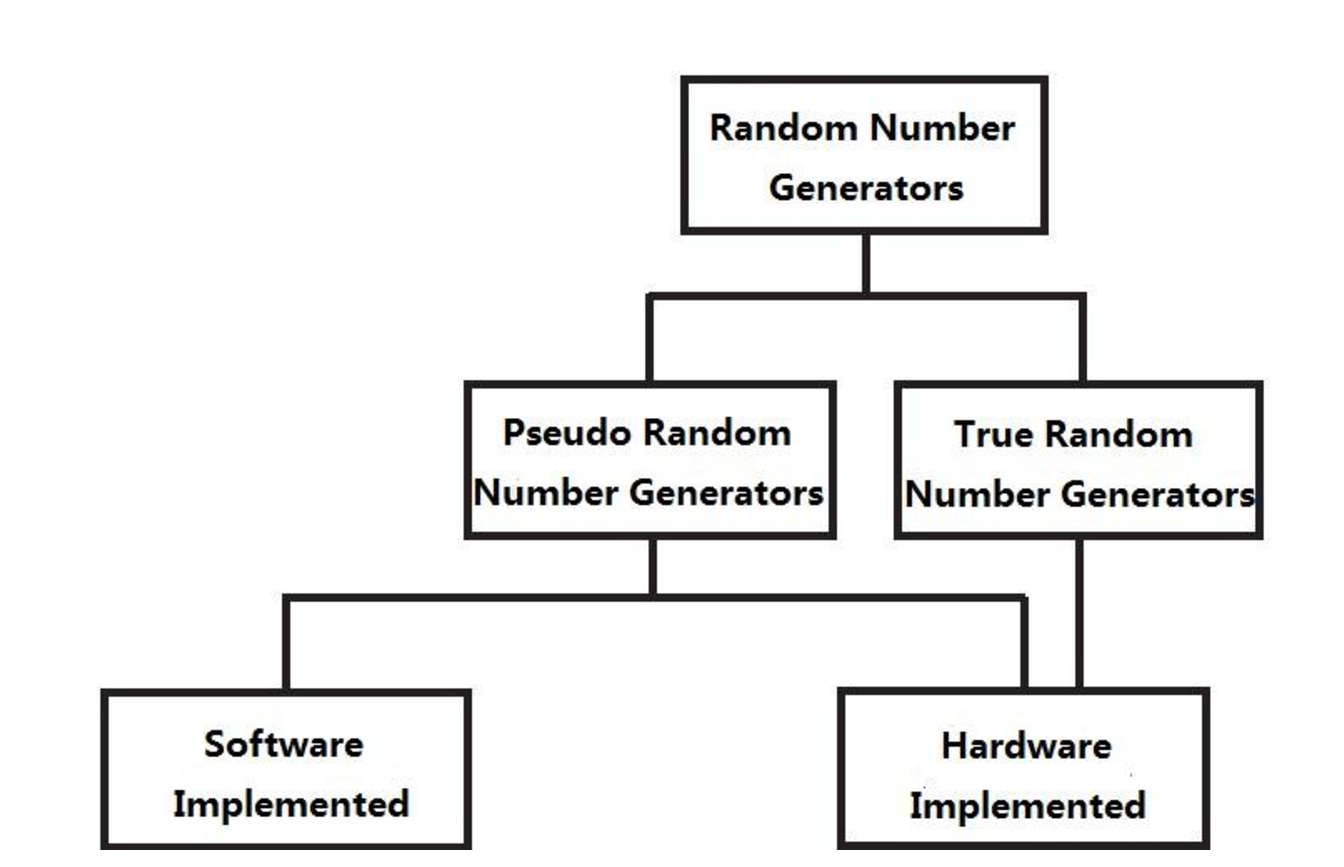
\includegraphics[width=3.85in]{Classification.eps}
\DeclareGraphicsExtensions.
\caption{Classification of random number generators}
\label{Classification}
\end{figure}



\subsection{True Random Number Generators (TRNGs)}
A TRNG is a physical device that generates statistically independent and unbiased bits. They are also
called non-deterministic RNGs. Such devices, which
exist too in computers, are often based on microscopic phenomena that generate a low-level, statistically random ``noise'' signal, such as thermal noise, photoelectric effect, or any other quantum phenomena. These processes are, in theory, completely unpredictable, and the theory's assertions of unpredictability are subject to experimental test. 

A quantum-based hardware random number generator typically consists in a transducer that converts some aspect of a given physical phenomena, into an electrical signal. An amplifier and other electronic circuitry bring the output of the transducer into the macroscopic realm, and some analog to digital converter translates the output into a digital number, often a simple binary digit 0 or 1. By repeatedly sampling the randomly varying signal, a series of random numbers is thus obtained.

\subsection{Pseudo Random Number Generators (PRNGs)}

A pseudorandom number generator (PRNG), also known as deterministic random bit generator (DRBG), is an algorithm for generating a sequence of numbers that approximates the properties of random numbers~\cite{Barker05recommendationfor}. The sequence is not truly random in that it is completely determined by a relatively small set of initial values, called the PRNG's state. Although sequences that are closer to truly random can be generated using hardware random number generators, pseudorandom numbers are important in practice for simulations (e.g., of physical systems with the Monte Carlo method), and are central in   cryptography and procedural generation due to their fundamental property of reproductibility. 

Common classes of these algorithms are linear congruential generators, Lagged Fibonacci generators, linear feedback shift registers, feedback with carry shift registers, and generalized feedback shift registers. Recent instances of pseudorandom algorithms include Blum Blum Shub, Fortuna, and the Mersenne twister.
All these generators will be developed later in this manuscript.

%\section{Cryptographically secure pseudo random number generators}
%
%
%A PRNG suitable for cryptographic applications is called a cryptographically secure PRNG (CSPRNG). A requirement for a CSPRNG is that an adversary not knowing the seed has only negligible advantage in distinguishing the generator's output sequence from a random sequence. In other words, while a PRNG is only required to pass certain statistical tests, a CSPRNG must pass all statistical tests that are restricted to polynomial time in the size of the seed. Though such property cannot be proven, strong evidence may be provided by reducing the CSPRNG to a known hard problem in mathematics (e.g., integer factorization). In general, years of review may be required before an algorithm can be certified as a CSPRNG.
%
%Some classes of CSPRNGs include the following:
%\begin{itemize}
%
%\item     Stream ciphers
%\item     Block ciphers running in counter or output feedback mode.
%\item     PRNGs that have been designed specifically to be cryptographically secure, such as Microsoft's Cryptographic 
% Application Programming Interface function CryptGenRandom, the Yarrow algorithm (incorporated in Mac OS X and FreeBSD), and Fortuna.
%\item     Combination PRNGs which attempt to combine several PRNG primitive algorithms with the goal of removing any non-randomness.
%\item     Special designs based on mathematical hardness assumptions. Examples include Micali-Schnorr and the Blum Blum Shub algorithm, which provide a strong security proof. Such algorithms are rather slow compared to traditional constructions, and impractical for many applications.
% 
%\end{itemize}

%\section{Stream Cipher}
%A stream cipher generates successive elements of the keystream based on an internal state. This state is updated in essentially two ways: if the state changes independently of the plaintext or ciphertext messages, the cipher is classified as a synchronous stream cipher. By contrast, self-synchronising stream ciphers update their state based on previous ciphertext digits.
%
%\subsection{One-Time Pad (Vernam Cipher)}
%In modern terminology, a Vernam cipher is a stream cipher in which the plaintext is XORed with a random or pseudorandom stream of data (the keystream) of the same length to generate the ciphertext. If the keystream is truly random and used only once, this is effectively a one-time pad. 
%
%Shannon~\cite{shannon-otp} showed that the one-time pad provides perfect security. This means
%that the conditional entropy of the message $M$ knowing the ciphertext $C$ is the same as the
%entropy of the original message, i.e. $H(M|C) = H(M)$. He also showed that the one-time
%pad is optimal in the sense that the previous conditions cannot be achieved with a key of
%size smaller than the message.
%
%The problem of the one-time pad is that we first have to agree on a key of the same
%length as the message. For most applications this is not practical. The next two schemes
%try to produce a ``random looking`` keystream from a short key and IV. By random looking,
%we mean that we cannot distinguish the keystream from a random sequence in a complexity
%less than trying all possible keys.
%
%\subsection{Synchronous stream ciphers}
%In a synchronous stream cipher a stream of pseudorandom digits is generated independently of the plaintext and ciphertext messages, and then combined with the plaintext (to encrypt) or the ciphertext (to decrypt). In the most common form, binary digits are used (bits), and the keystream is combined with the plaintext using the exclusive or operation (XOR). This is termed a binary additive stream cipher.
%
%In a synchronous stream cipher, the sender and receiver must be exactly in step for decryption to be successful. If digits are added or removed from the message during transmission, synchronisation is lost. To restore synchronisation, various offsets can be tried systematically to obtain the correct decryption. Another approach is to tag the ciphertext with markers at regular points in the output.
%
%If, however, a digit is corrupted in transmission, rather than added or lost, only a single digit in the plaintext is affected and the error does not propagate to other parts of the message. This property is useful when the transmission error rate is high; however, it makes it less likely the error would be detected without further mechanisms. Moreover, because of this property, synchronous stream ciphers are very susceptible to active attacks -- if an attacker can change a digit in the ciphertext, he might be able to make predictable changes to the corresponding plaintext bit; for example, flipping a bit in the ciphertext causes the same bit to be flipped in the plaintext.
%
%\subsection{Self-synchronizing stream ciphers}
%Another approach uses several of the previous N ciphertext digits to compute the keystream. Such schemes are known as self-synchronizing stream ciphers, asynchronous stream ciphers or ciphertext autokey (CTAK). The idea of self-synchronization was patented in 1946, and has the advantage that the receiver will automatically synchronise with the keystream generator after receiving N ciphertext digits, making it easier to recover if digits are dropped or added to the message stream. Single-digit errors are limited in their effect, affecting only up to N plaintext digits.
%
%An example of a self-synchronising stream cipher is a block cipher in cipher feedback (CFB) mode.
%


\subsection{Chaos-based Random Number Generators}

Since the seventies in last century, the use of chaotic dynamics for the generation of random sequences has raised a lot of interests. It is clearly pointed out by some researchers that there exists a close relationship between chaos and randomness, and many works have been witnessed in the last two decades~\cite{Provenzale199231}.
To do so, chaotic dynamics are usually studied in two different domains, depending on whether the generator is an hardware or a software one.
\begin{itemize}
 \item Continuous time domain: chaotic dynamics generated by differential equations.
 \item Discrete time domain: recurrent sequences using chaotic maps.
\end{itemize}

Chaos possesses several distinct properties that can possibly give meaning to the desire to use such dynamics for generating pseudorandomness, namely: the sensitivity to initial conditions, the ergodicity, the wide band spectrum, and the unpredictable and random-like behavior of iterates.
Although it is still controversy to equate these properties with randomness and claim a chaos-based random number generator to be good enough, a lot of designs and applications, in particular related to communications securing, have been proposed.

Nowadays, it is common to use a chaotic map for pseudorandom number generation. Due to the recent design of electronic circuits for the realization of chaotic systems, it is also possible to generate the bit sequence by observing such dynamics, as a replacement of those physical random sources.

\section{Statistical Tests for Randomness}
\label{Some famous statistical tests of random number generators}

A theoretical proof for the randomness of a generator is impossible to give, as such proof requires first to mathematically define what is randomness. Therefore statistical inference based on observed sample sequences produced by the generator seems to be the best option. Considering the properties of binary
random sequences, various statistical tests can be designed to evaluate the assertion
that the sequence is generated by a perfectly random source. 
We have performed certain statistical tests for various CI PRNGs we proposed. These tests
include TestU01~\cite{Lecuyer2009}, NIST suite~\cite{ANDREW2008},
DieHARD battery of tests~\cite{Marsaglia1996}, and Comparative test parameters. For completeness and for reference, we give
in the following subsection a brief description of each of the
aforementioned tests.



\subsection{NIST statistical test suite}



Among the numerous standard tests for pseudo-randomness, a convincing way to show the randomness of the produced sequences is to confront them to the NIST (National Institute of Standards and Technology) Statistical Test, because it is an up-to-date test suite proposed by the Information Technology Laboratory (ITL). A new version of the Statistical Test Suite (Version 2.0) has been released in August 11, 2010.


The NIST test suite SP 800-22 is a statistical package consisting of 15 tests. They were developed to test the randomness of binary sequences produced by hardware or software based cryptographic PRNGs. These tests focus on a variety of different types of non-randomness that could exist in a sequence. 


For each statistical test, a set of $p-values$ (corresponding to the set of sequences) is produced. The interpretation of empirical results can be conducted in any number of ways. In this manuscript, the examination of the distribution of $p-values$ to check for uniformity ($p-value_{T}$) is used:
the distribution of $P-values$ is examined to ensure uniformity. 
Concretely, this demand is verified in an usual way as follows: if $p-value_{T} \geqslant 0.0001$, then the sequences can be considered to be uniformly distributed.

In our experiments, 100 sequences (s = 100), each with 1,000,000-bit long, are generated and tested. If the $p-value_{T}$ of any test is smaller than 0.0001, the sequences are considered to be not good enough and the generating algorithm is not suitable for usage.

In what follows, the fifteen tests of the NIST Statistical tests suite, are recalled. A more detailed description for those tests could be found in \cite{ANDREW2008}.
\begin{itemize}
\item \textbf{Frequency (Monobit) Test (FT)} is to determine whether the number of ones and zeros in a sequence are approximately the same as would be expected for a truly random sequence.


\item \textbf{Frequency Test within a Block (FBT)} is to determine whether the frequency of ones in an M-bit block is approximately $M/2$, as would be expected under an assumption of randomness. %($M$ is the length of each block.)


\item \textbf{Runs Test (RT)} is to determine whether the number of runs of ones and zeros of various lengths is as expected for a random sequence. In particular, this test determines whether the oscillation between such zeros and ones is too fast or too slow.


\item \textbf{Test for the Longest Run of Ones in a Block (LROBT)} is to determine whether the length of the longest run of ones within the tested sequence is consistent with the length of the longest run of ones that would be expected in a random sequence.


\item \textbf{Binary Matrix Rank Test (BMRT)} is to check for linear dependence among fixed length substrings of the original sequence.


\item \textbf{Discrete Fourier Transform (Spectral) Test (DFTT)} is to detect periodic features (i.e., repetitive patterns that are near each other) in the tested sequence that would indicate a deviation from the assumption of randomness.


\item \textbf{Non-overlapping Template Matching Test (NOTMT)} is to detect generators that produce too many occurrences of a given non-periodic (aperiodic) pattern.


\item \textbf{Overlapping Template Matching Test (OTMT)} is to check the number of occurrences of pre-specified target strings.

\item \textbf{Maurer's ``Universal Statistical'' Test (MUST)} is to detect whether or not the sequence can be
significantly compressed without loss of information.

\item \textbf{Linear Complexity Test (LCT)} is to determine whether or not the sequence is complex enough to be considered random.

\item \textbf{Serial Test (ST)} is to determine whether the number of occurrences of the $2^{m}$ $m$-bit
overlapping patterns is approximately the same as would be expected for a random sequence.

\item \textbf{Approximate Entropy Test (AET)} is to compare the frequency of overlapping blocks of two consecutive/adjacent lengths (m and m+1) against the expected result for a random sequence.%(m is the length of each block.)

\item \textbf{Cumulative Sums (Cusum) Test (CST)} is to determine whether the cumulative sum of the partial sequences occurring in the tested sequence is too large or too small relative to the expected behavior of that cumulative sum for random sequences.

\item \textbf{Random Excursions Test (RET)} is to determine if the number of visits to a particular state within a cycle deviates from what one would expect for a random
sequence.

\item \textbf{Random Excursions Variant Test (REVT)} is to detect deviations from the expected number
of visits to various states in the random walk.
\end{itemize}

\subsection{DieHARD battery of tests}
The DieHARD battery of tests was developed in 1996 by Prof. Georges Marsaglia
from the Florida State University for testing randomness of sequences of numbers \cite{Marsaglia1996}. 
It has been the most sophisticated standard for over a decade. Because of the stringent requirements in the DieHARD test suite, a generator passing DieHARD battery of 
tests can be considered good as a rule of thumb. It was supposed to give a better way of analysis in comparison to original FIPS statistical tests.

The DieHARD battery of tests consists of 18 different independent statistical tests. 
Each test requires binary file of about 10-12 million bytes in order to run the full set of tests. 
As the NIST test suite, most of the tests in DieHARD return a $p-value$, which should be uniform on $[0,1)$ if the input file 
contains truly independent random bits. Those $p-values$ are obtained by
$p=F(X)$, where $F$ is the assumed distribution of the sample random variable $X$ (often normal). 
But that assumed $F$ is just an asymptotic approximation, for which the fit will be worst 
in the tails. Thus occasional $p-value$s near 0 or 1, such as 0.0012 or 0.9983 can occur. Unlike the NIST test suite, the test is considered to be successful when
the $p-value$ is in range $[0 + \alpha , 1 -\alpha ]$,
where $\sqrt{\alpha}$ is the level of significance of the test.

For example, with a level of significance of $5\%$, $p-values$ are expected to be in
$[0.025, 0.975]$. Note that if the $p-value$ is not in this range, it means that the null
hypothesis for randomness is rejected even if the sequence is truly random. These
tests are:
\begin{itemize}
\item \textbf{Birthday Spacings.} Choose random points on a large interval. The spacings
between the points should be asymptotically Poisson distributed. The name
is based on the birthday paradox.
\item \textbf{Overlapping Permutations.} Analyze sequences of five consecutive random
numbers. The 120 possible orderings should occur with statistically equal
probability
\item \textbf{Ranks of matrices.} Select some number
of bits from some number of random numbers to form a matrix over 0,1, then
determine the rank of the matrix. Count the ranks.
\item \textbf{Monkey Tests.} Treat sequences of some number of bits as ``words''. Count
the overlapping words in a stream. The number of ``words'' that don't appear
should follow a known distribution. The name is based on the infinite monkey
theorem.
\item \textbf{Count the 1's.} Count the 1 bits in each of either successive
or chosen bytes. Convert the counts to ``letters'', and count the occurrences
of five-letter ``words''
\item \textbf{Parking Lot Test.} Randomly place unit circles in a $100 \times 100 $ square. If the
circle overlaps an existing one, try again. After 12,000 tries, the number of
successfully ``parked'' circles should follow a certain normal distribution.
\item \textbf{Minimum Distance Test.} Randomly place 8,000 points in a $10,000 \times 10,000$ 
square, then find the minimum distance between the pairs. The square of this
distance should be exponentially distributed with a certain mean.
\item \textbf{Random Spheres Test.} Randomly choose 4,000 points in a cube of edge 1,000.
Center a sphere on each point, whose radius is the minimum distance to another point. The smallest sphere's volume should be exponentially distributed
with a certain mean.
\item \textbf{The Sqeeze Test.} Multiply 231 by random floats on [0,1) until you reach 1.
Repeat this 100,000 times. The number of floats needed to reach 1 should
follow a certain distribution.
\item \textbf{Overlapping Sums Test.} Generate a long sequence of random floats on [0,1).
Add sequences of 100 consecutive floats. The sums should be normally distributed with characteristic mean and sigma.
\item \textbf{Runs Test.} Generate a long sequence of random floats on [0,1). Count ascending and descending runs. The counts should follow a certain distribution.
\item \textbf{The Craps Test.} Play 200,000 games of craps, counting the wins and the number
of throws per game. Each count should follow a certain distribution.
\end{itemize}

\subsection{ENT test program}
%
ENT test program applies various tests to sequences of bytes stored in
files and reports the results of those tests. The program is useful
for evaluating random number generators for encryption and statistical
sampling applications, compression algorithms, and other applications
where the information density of a file is of interest~\cite{ent}.

There are 5 tests contained in the program:
%
\begin{enumerate}
\item Entropy test: Entropy testing, in bits per character (or byte), which
  corresponds to the incompressibility of the sequence (as a perfectly
  random sequence cannot be compressed, since no part of it can be
  expressed in terms of other parts). Hence entropy of 8 bits/byte
  means perfect randomness in the sense of incompressibility.
\item $\chi^2$ test: $\chi^2$ testing is very common for
  goodness-of-fit of sample distributions of random numbers. It is
  known to be very sensitive to deficiencies in random number
  generators (when it is located between 5\% to 95\%, data are treated
  as random).
\item Sample test: Sample test means can be tested for bias in random
  number generation. In binary mode, the expected mean is 0.5 while
  for bytes, the expected mean is 127.5.
\item Monte Carlo test: a Monte Carlo approximation of $\pi$, which is
  simply the evaluation the area of the unit circle using the $N$
  generated random numbers ($X_i$,$X_{i-1}$), $i = 2,...,N$.
\item Serial Correlation test: Serial correlation coefficient
  evaluated from $<X_i,X_{i-1}>/<X_i,X_i>$, for $i=2,..N$. The
  intended value for perfect random sequences is 0.
\end{enumerate}

\subsection{Comparative test parameters}

In this section, five well-known statistical tests~\cite{Menezes1997} are presented to play the role of easily verifiable comparison tools. They encompass frequency and autocorrelation tests. In what follows, $s = s^0,s^1,s^2,\dots , s^{n-1}$ denotes a binary sequence of length $n$. The question is to determine whether this sequence possesses some specific characteristics that a truly random sequence would be likely to exhibit. 


\paragraph{Frequency test (monobit test)}

The purpose of this test is to check if the numbers of 0's and 1's are approximately equal in $s$, as it would be expected for a random sequence. Let $n_0, n_1$ denote these numbers. The statistic used here is 
\begin{equation*}
X_1=\frac{(n_0-n_1)^2}{n}, 
\end{equation*}
which approximately follows a $\chi^2$ distribution with one degree of freedom when $n\geqslant 10^7$.

\paragraph{Serial test (2-bit test)}

The purpose of this test is to determine if the number of occurrences of 00, 01, 10, and 11 as subsequences of $s$ are approximately the same. Let $n_{00} , n_{01} ,n_{10}$, and $n_{11}$ denote the number of occurrences of $00, 01, 10$, and $11$ respectively. Note that $n_{00} + n_{01} + n_{10} + n_{11} = n-1$ since the subsequences are allowed to overlap. The
statistic used here is:
\begin{equation*}
X_2=\frac{4}{n-1}(n_{00}^2+n_{01}^2+n_{10}^2+n_{11}^2)-\frac{2}{n}(n_0^2+n_1^2)+1,
\end{equation*}
 which approximately follows a $\chi^2$ distribution with 2 degrees of freedom if $n\geqslant 21$.

\paragraph{Poker test}

The poker test studies if each pattern of length $m$ (without overlapping) appears the same number of times in $s$. Let $\lfloor \frac{n}{m} \rfloor\geqslant 5 \times 2^m$ and $k= \lfloor \frac{n}{m} \rfloor $. Divide the sequence $s$ into $k$ non-overlapping parts, each of length $m$. Let $n_i$ be the number of occurrences of the $i^{th}$ type of sequence of length $m$, where $1 \leqslant i \leqslant 2^m$. The statistic used is 
\begin{equation*}
X_3=\dfrac{2^m}{k}\left(\displaystyle{\sum^{2^m}_{i=1}n^2_i}\right)-k,
\end{equation*}
which approximately follows a $\chi^2$ distribution with $2^m-1$ degrees of freedom. Note that the poker test is a generalization of the frequency test (setting $m = 1$ in the poker test yields the frequency test).

\paragraph{Runs test}

The purpose of the runs test is to figure out whether the number of runs of various lengths in the sequence $s$ is as expected, for a random sequence. A run is defined as a pattern of all zeros or all ones, a block is a run of ones, and a gap is a run of zeros. The expected number of gaps (or blocks) of length $i$ in a random sequence of length $n$ is $e_i = \frac{n-i+3}{2^{i+2}}$. Let $k$ be equal to the largest integer $i$ such that $e_i \geqslant 5$. Let
$B_i , G_i$ be the number of blocks and gaps of length $i$ in $s$, for each $i \in \llbracket 1, k\rrbracket$. The statistic used here will then be:
\begin{equation*}
\displaystyle{X_4=\sum^k_{i=1}\frac{(B_i-e_i)^2}{e_i}+\sum^k_{i=1}\frac{(G_i-e_i)^2}{e_i}},
\end{equation*}
\noindent which approximately follows a $\chi^2$ distribution with $2k - 2$ degrees of freedom.

\paragraph{Autocorrelation test}

The purpose of this test is to check for coincidences between the sequence $s$ and (non-cyclic) shifted versions of it. Let $d$ be a fixed integer, $ 1 \leqslant d \leqslant \lfloor n/2 \rfloor$. The value $A(d) = \sum_{i=0}^{n-d-1} s_i\oplus s_{i+d}$ is the amount of bits not equal between the sequence and itself displaced by $d$ bits. The statistic used is:
\begin{equation*}
X_5=\dfrac{2 \left(A(d)-\frac{n-d}{2}\right)}{\sqrt{n-d}},
\end{equation*}
which approximately follows a normal distribution $\mathcal{N}(0, 1)$ if $n-d \geqslant 10$. Since small values of $A(d)$ are as unexpected as large values, a two-sided test should be used.

\subsection{TestU01 Statistical Test}
\label{Testing a generator}

TestU01 is extremely diverse in implementing classical tests,
cryptographic tests, new tests proposed in the literature, and original tests.
In fact, it encompasses most of the other testsuites. 
There are seven batteries of tests in the TestU01 package, which are listed in what follows:

\begin{itemize}
\item{\textbf{SmallCrush.}} The first battery to check, with 15 $p-$values reported. This is a fast collection of tests used to be sure that the basic requirements of randomness are satisfied. In case of success, this battery should be followed by Crush and BigCrush.
\item{\textbf{Crush.}} This battery includes many difficult tests, like those described in~\cite{Knuth1998}. %Cette référence n'apparaît pas.
%D. E. Knuth. The Art of Computer Programming, Volume 2: Seminumerical Algorithms. Addison-Wesley, Reading, Mass., third edition, 1998.
It uses approximately $2^{35}$ random numbers and applies 96 statistical tests
(it computes a total of 144 test statistics and $p-values$).
\item{\textbf{BigCrush.}} The BigCrush uses
approximately $2^{38}$ random numbers and applies 106 tests (it computes 160 test
statistics and $p-values$). 
A suite of very stringent statistical tests, and the most difficult battery to pass.
\item{\textbf{Rabbit.}} This battery of tests reports 38 $p-values$.
\item{\textbf{Alphabit.}} Alphabit and AlphabitFile have been designed primarily to test hardware random bits generators. 17 $p-values$ are reported here.
\item{\textbf{Pseudo-DieHARD.}} This battery implements most of the tests contained in the popular battery DieHARD or, in some cases, close approximations to them. It is not a very stringent battery. Indeed, there is no generator that can pass Crush and BigCrush batteries and fail Pseudo-DieHARD, while the converse occurs for several defective generators. 126 $p-values$ are reported here.
\item{\textbf{FIPS\_140\_2.}} As recalled previously, the NIST (National Institute of Standards and Technology) of the U.S. federal government has proposed a statistical test suite. It is used to evaluate the randomness of bitstreams produced by cryptographic random number generators. This battery reports 16 $p-values$.
\end{itemize}

Six predefined batteries of tests are available in TestU01; three of them
are for sequences of $\mathcal{U}(0, 1)$ random numbers and the three others are for bit
sequences. In the first category, we have SmallCrush, Crush, and BigCrush.

To test a RNG for general use,
one could first apply the small and fast battery SmallCrush. If it passes, one could then apply
the more stringent battery Crush, and finally the yet more time-consuming battery BigCrush.
These batteries of tests include the classical tests described in Knuth~\cite{Knuth1998}, for
example: the run, poker, coupon collector, gap, max-of-t, and permutation tests.
There are collision and birthday spacings tests in 2, 3, 4, 7, 8 dimensions, several close pairs tests in 2, 3, 5, 7, 9 dimensions, and correlation tests. Some
tests use the generated numbers as a sequence of ``random'' bits: random walk
tests, linear complexity tests, a Lempel-Ziv compression test, several Hamming
weights tests, matrix rank tests, run and correlation tests, among others.




The batteries Rabbit, Alphabit, and BlockAlphabit are for binary sequences
(e.g., a cryptographic pseudorandom generator or a source of random bits
produced by a physical device). They were originally designed to test a finite
sequence contained in a binary file. When invoking the battery, one must specify the number $n_B$ of bits available for each test. When the bits are in a file, $n_B$
must not exceed the number of bits in the file, and each test will reuse the same
sequence of bits starting from the beginning of the file (so the tests are not independent). When the bits are produced by a generator, each test uses a different
stream. In both cases, the parameters of each test are chosen automatically as
a function of $n_B$ .
The batteries Alphabit and Rabbit can be applied on a binary file considered as a source
of random bits. They can also be applied on a programmed generator. Alphabit has been
defined primarily to test hardware random bits generators. The battery PseudoDieHARD
applies most of the tests in the well-known DieHARD suite of Marsaglia [106]. The battery
FIPS\_140\_2 implements the small suite of tests of the FIPS\_140\_2 standard from NIST.
The batteries described in this module will write the results of each test (on standard
output) with a standard level of details (assuming that the Boolean switches of module
swrite have their default values), followed by a summary report of the suspect p-values
obtained from the specific tests included in the batteries. It is also possible to get only the
summary report in the output, with no detailed output from the tests, by setting the Boolean
switch swrite\_Basic to FALSE. Rabbit and Alphabit apply 38 and 17 different statistical tests,
respectively. 

Some of the tests compute more than one statistic (and $p-value$) using the same stream of random
numbers and these statistics are thus not independent. That is why the number of statistics
in the summary reports is larger than the number of tests in the description of the batteries.
For a more detailed description, the reader is referred
to the documentation of the TestU01 library.

\begin{itemize}
\item{\textbf{Small Crush:}}\\smarsa\_BirthdaySpacings \\ 
 sknuth\_Collision \\ 
 sknuth\_Gap\\ 
 sknuth\_SimpPoker \\ 
 sknuth\_CouponCollector\\ 
 sknuth\_MaxOft \\ 
 svaria\_WeightDistrib \\ 
 smarsa\_MatrixRank \\
 sstring\_HammingIndep\\ 
 swalk\_RandomWalk1\\ 
\item{\textbf{Crush:}}\\smarsa\_SerialOver \\
 smarsa\_CollisionOver\\ 
 smarsa\_BirthdaySpacings\\ 
 snpair\_ClosePairs\\ 
 snpair\_ClosePairsBitMatch \\
 sknuth\_SimpPoker\\ 
 sknuth\_CouponCollector\\ 
 sknuth\_Gap\\ 
 sknuth\_Run\\ 
 sknuth\_Permutation\\ 
 sknuth\_CollisionPermut\\ 
 sknuth\_MaxOft\\ 
 svaria\_SampleProd\\ 
 svaria\_SampleMean \\ 
 svaria\_SampleCorr\\ 
 svaria\_AppearanceSpacings \\
 svaria\_WeightDistrib \\
 svaria\_SumCollector\\ 
 smarsa\_MatrixRank\\ 
 smarsa\_Savir2\\ 
 smarsa\_GCD\\ 
 swalk\_RandomWalk1\\ 
 scomp\_LinearComp \\
 scomp\_LempelZiv\\ 
 sspectral\_Fourier3\\ 
 sstring\_LongestHeadRun \\
 sstring\_PeriodsInStrings\\ 
 sstring\_HammingWeight2\\ 
 sstring\_HammingCorr\\ 
 sstring\_HammingIndep \\
 sstring\_Run\\ 
 sstring\_AutoCor \\ 
\item{\textbf{Big Crush:}}\\smarsa\_SerialOver\\ 
smarsa\_CollisionOver\\ 
smarsa\_BirthdaySpacings\\ 
snpair\_ClosePairs \\ 
sknuth\_SimpPoker\\ 
sknuth\_CouponCollector\\ 
sknuth\_Gap\\ 
sknuth\_Run\\ 
sknuth\_Permutation\\ 
sknuth\_CollisionPermut\\ 
sknuth\_MaxOft\\ 
svaria\_SampleProd\\ 
svaria\_SampleMean\\ 
svaria\_SampleCorr\\ 
svaria\_AppearanceSpacings\\ 
svaria\_WeightDistrib\\ 
svaria\_SumCollector\\ 
smarsa\_MatrixRank\\ 
smarsa\_Savir2\\ 
smarsa\_GCD\\ 
swalk\_RandomWalk1\\ 
scomp\_LinearComp\\ 
scomp\_LempelZiv\\ 
sspectral\_Fourier3\\ 
sstring\_LongestHeadRun\\ 
sstring\_PeriodsInStrings\\ 
sstring\_HammingWeight2\\ 
sstring\_HammingCorr\\ 
sstring\_HammingIndep\\ 
sstring\_Run\\ 
sstring\_AutoCor\\ 

\item{\textbf{Rabbit:}}\\smultin\_MultinomialBitsOver\\ 
snpair\_ClosePairsBitMatch\\ 
svaria\_AppearanceSpacings\\ 
scomp\_LinearComp\\ 
scomp\_LempelZiv\\ 
sspectral\_Fourier1\\ 
sspectral\_Fourier3\\ 
sstring\_LongestHeadRun\\ 
sstring\_PeriodsInStrings\\ 
sstring\_HammingWeight\\ 
sstring\_HammingCorr\\ 
sstring\_HammingIndep\\ 
sstring\_AutoCor\\ 
sstring\_Run\\ 
smarsa\_MatrixRank\\ 
swalk\_RandomWalk1\\ 

\item{\textbf{Alphabit:}}\\smultin\_MultinomialBitsOver\\ 
sstring\_HammingIndep\\ 
sstring\_HammingCorr\\ 
swalk\_RandomWalk1 \\ 


\item{\textbf{Pseudo-DieHARD:}}\\Birthday Spacings test\\ 
Overlapping 5-Permutation test\\ 
Binary Rank Tests for Matrices test\\ 
Bitstream test\\ 
OPSO test\\ 
OQSO test\\ 
DNA test\\ 
Count-the-1's test\\ 
Parking Lot test\\ 
Minimum Distance test\\ 
3-D Spheres test\\ 
Squeeze test\\ 
Overlapping Sums test\\ 
Runs test\\ 
Craps test\\ 

\item{\textbf{FIPS\_140\_2:}}\\Monobit test\\ 
``poker'' test\\ 
Runs test\\ 
Longest Run of Ones in a Block test

\end{itemize}

TestU01 suite implements hundreds of tests and reports $p-$values. If a $p-$value is within $[0.001,0.999]$, the associated test is a success. A $p-$value lying outside this boundary means that its test has failed. %This is the standard range the test-suite suggests. The p-value selection criteria for the various test suites were chosen to produce a few failures in the best cases. Setting the criteria too low (closer to zero) would exhibit no failures and setting the criteria too high would fail everything.




\section{FPGA}
We finally introduce the field-programmable gate array (FPGA) architecture, on which our generators will be
implemented. 

A FPGA is an integrated circuit designed to be configured by a customer or a designer after manufacturing-hence ``field-programmable'' 
\begin{figure}
\centering
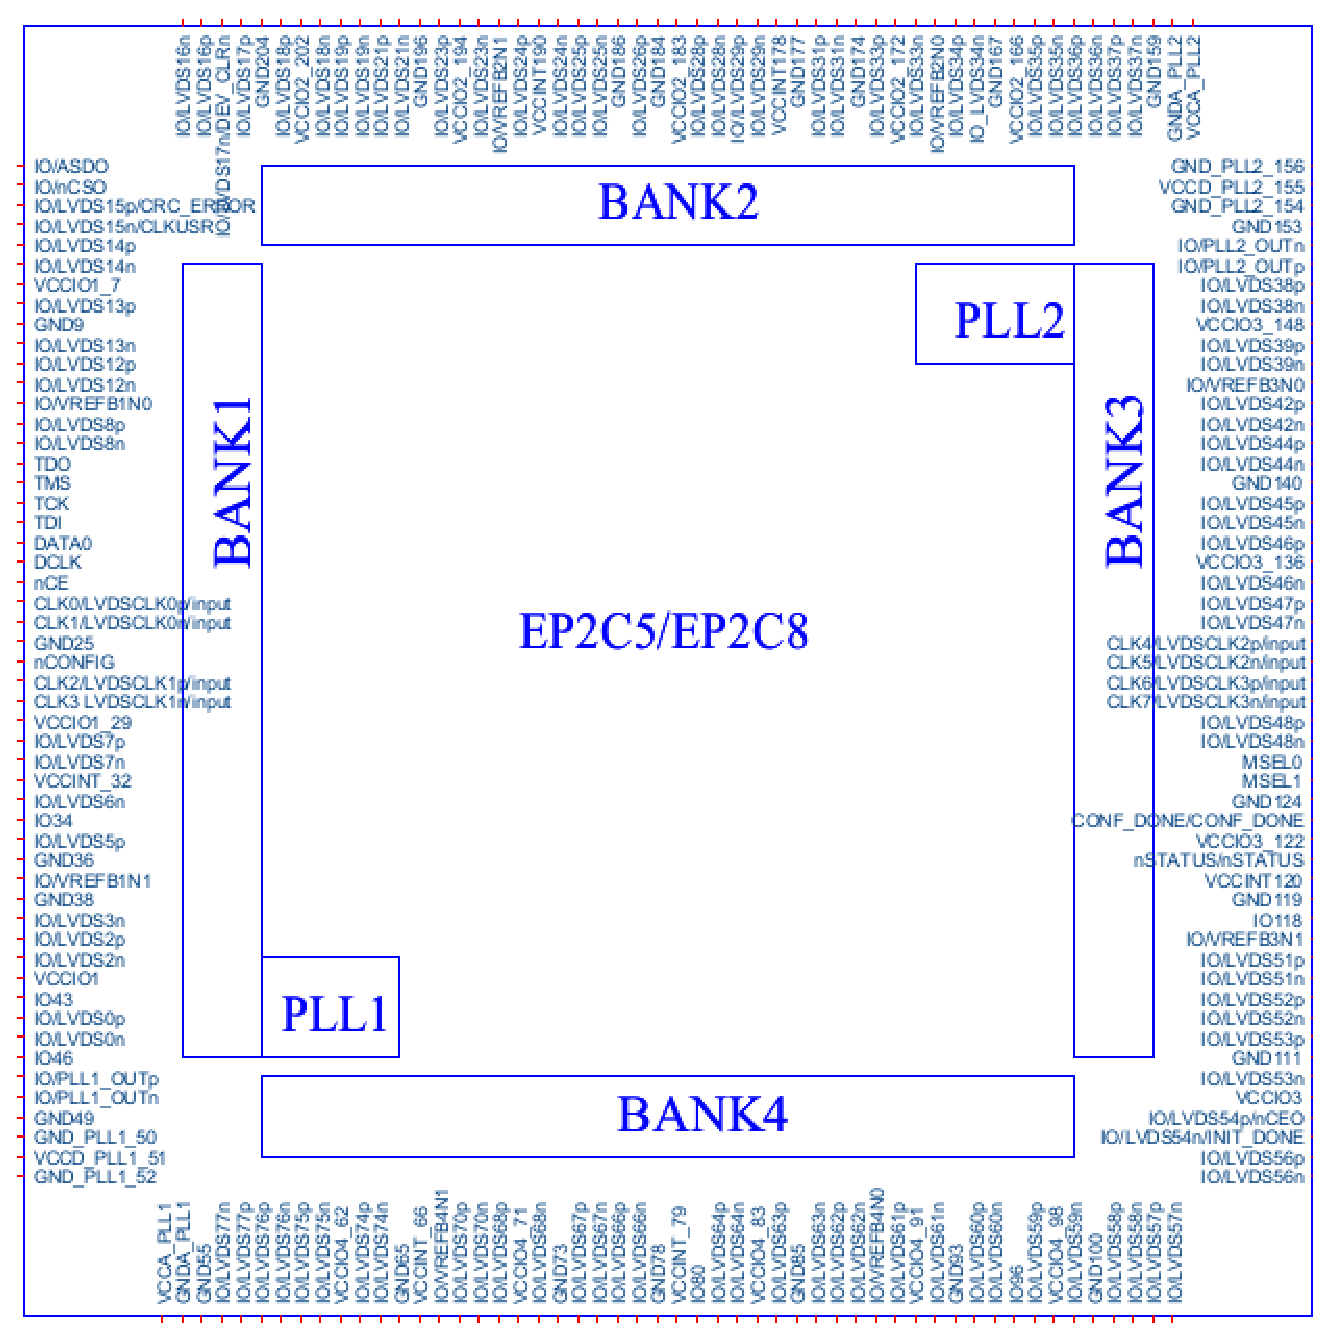
\includegraphics[width=5in]{fpga_scheme.eps}
\DeclareGraphicsExtensions.
\caption{FPGA EP2C8 core from ALTERA company}
\label{fpga_scheme}
\end{figure}
%The experiments in this research were implemented on FPGA. 
(a FPGA is indeed a VLSI chip with some special features).
The most common FPGA architecture consists of an array of logic blocks (called Configurable Logic Block, CLB, or Logic Array Block, LAB, depending on vendor), I/O pads, and routing channels. Generally, all the routing channels have the same width (number of wires). Multiple I/O pads may fit into the height of one row or the width of one column in the array. There are some primitives such as lookup tables (LUT) and flip-flop (FF) inside the CLB. The functions of these primitives and connections between them can be configured for different designs. Programmable routing matrices (PRM), implemented in static RAMs, are used to connect the I/O ports of the CLBs.

The advantages of FPGA designs over traditional VLSI designs are:
\begin{itemize}
\item The feasibility of reusing fast design to product time and chips for different designs.
\item Easy simulation and debugging. Software simulator and debugger provide
efficient methods of finding bugs and estimating of performance.
\item Low cost prototyping for early designs.
\item Design can be upgraded after deployment without hardware replacement.
\item Developing  hardware  systems  using  design  tools  for  FPGA  is  as  easy  as developing a software system.
\item FPGA can be reprogrammed on the field. 
\end{itemize}

To define the behavior of the FPGA, the user provides a hardware description language (HDL) or a schematic design. The most common HDLs are VHDL and Verilog, although in an attempt to reduce the complexity of designing in HDLs, which have been compared to the equivalent of assembly languages, there are moves to raise the abstraction level through the introduction of alternative languages. 

A general structure outline of FPGA core (EP2C8) used in this thesis is shown in Fig.\ref{fpga_scheme}



\part{Pseudorandom Number Generator Based on Chaotic Iteration}
\label{Pseudo Random Number Generator Based on Chaotic Iteration}
\chapter{Computer Science RNGs: an Introduction}
\label{Introduction}
\minitoc
Alone with the rapid development of Internet and universal application of multimedia technology, multimedia data including audio, image, and video has been transmitted over insecure channels, it implies the need to protect data and privacy in digital world. This development has revealed new major security issues. For example, new security concerns have recently appeared because of the evolution of the Internet to support such activities as e-Voting, VoD, and digital rights management~\cite{Zhu200675}. The random number generators  are very important cryptographic primitive widely used in the Internet security, because they are fundamental in cryptosystems and information hiding schemes. 

RNGs are widely used in science and technology, it is a critical component in modern cryptographic systems, communication systems, statistical simulation systems, and any scientific area incorporating Monte Carlo methods and many others \cite{quantum,communication,cryptography}. The random statistical quality of the generated bit sequence is measured by two aspects: the unpredictability of the bit stream and the speed at which the random bits can be produced.  Other factors like system complexity, cost, reliability and so on, are also important for establishing successful RNGs. As stated before, there are usually two methods for random numbers generation. The first one, on which this part focuses, relates to deterministic algorithms implemented in hardware and software. In that context, pseudorandom numbers are degenerated from a single value called a ``seed'', and using an algorithm called pseudorandom number generator (PRNG~\cite{LEcuyer08}). The second approach, debated in the next part, counts on high entropy signals, either from purely non deterministic and stochastic physical phenomena, or from deterministic but chaotic dynamical systems (necessarily mixed with an unavoidable noisy and smaller compound~\cite{fast,dice}). A potential advantage of the latter physical high entropy signal, resides in its deterministic features which might be used to achieve chaos synchronization as it has been already demonstrated \cite{pecora:prl90} and widely used for secure chaos communications \cite{argyris:nat05}. However, synchronization possibility of the random binary sequence extracted from the chaotic physical signal is still an open problem, which resolution could lead to the efficient and practical use of the Vernam cypher.

For the PRNGs algorithms, they are majorly defined by a deterministic recurrent sequence in a finite state space, usually a finite field or ring, and an output function mapping each state to an input value. This is often either a real number in the interval $(0,1)$ or an integer in some finite range~\cite{LEcuyer08}. Such PRNGs can be easily implemented in any computational platform, however they suffer from the vulnerability that the future sequence can be deterministically computed if the seed or internal state of the algorithm is discovered. Additionally to their reproducible character, the main advantages of PRNGs is that no hardware cost is added and the speed is only counted on processing hardware. In 
a cryptographic context, these algorithms are developed to prevent guessing of the initial conditions, thus their speed are slowed down due to the increased complexity of such precaution.

Recently, some researchers have demonstrated the possibility to use chaotic dynamical systems as RNGs to reinforce the security of cryptographic algorithm, due to the unpredictability and distort-like property of chaotic dynamical systems~\cite{Falcioni2005,Cecen2009,PO2004}. These attempts are related to the hypothesis that digital chaotic systems can possibly reinforce the security of cryptographic algorithms, because the behaviors of such systems are very similar to those of physical noise sources~\cite{Schuster1984}. For instance, in \cite{cite-key}, chaos has been applied to strengthen some optical communications. More generally, the random-like and unpredictable dynamics of chaotic systems, their inherent determinism and simplicity of realization suggest their potential for exploitation as RNGs.

In chaotic cryptography, there are two main design paradigms: in the first paradigm chaotic cryptosystems are realized in analog circuits (mainly based on chaos synchronization~\cite{PhysRevLett.64.821}) whereas in the second paradigm chaotic cryptosystems are realized in digital circuits or computers (synchronization is not an issue). Generally speaking, synchronization based chaotic cryptosystems are generally designed for securing communications though noisy channels, and they cannot be directly extended to design digital ciphers in pure cryptography. However, some cryptanalytic works have shown that most synchronization based chaotic cryptosystems are not really secure, since it is possible to extract some information on the secret chaotic parameters~\cite{BethLaMa94}. Therefore, although chaos synchronization is still actively studied in research of secure communications, as it is related in the next part
of this manuscript, the ideas underlying these approaches still remain disputed by conventional cryptographers. Since this dissertation is devoted to researches lying between chaotic cryptography and traditional cryptography, we will thus focus first on the second paradigm in this part of the dissertation. 

Even though chaotic systems exhibit random-like behavior, they are not necessarily cryptographically secure in their discretized form, see e.g.~\cite{HabutsuNSM91,Biham91cryptanalysisof}. The reason partly being that discretized chaotic functions do not automatically yield sufficiently complex behavior of the corresponding binary functions, which is, roughly speaking, a prerequisite for cryptographic security. It is therefore essential that the complexity of the binary functions is considered in the design phase such that necessary modifications can be made. Moreover, many suggested PRNG based on chaos suffer from reproducibility problems of the keystream due to the different handling of floating-point numbers on various processors, see e.g. \cite{Matthews:1984}.
Indeed, as outlined above, chaotic dynamical systems are usually continuous and hence defined on the real numbers domain. The transformation from real numbers to integers may lead to the loss of the chaotic behavior. The conversion to integers needs a rigorous theoretical foundation.

In this part, some new chaotic pseudorandom bit generator is presented, which can also be used to obtain numbers uniformly distributed between 0 and 1\footnote{Indeed, these bits can be grouped $n$ by $n$, to obtain the floating part of $x \in [0,1]$ represented in binary numeral system}. These generators are based on discrete chaotic iterations which satisfy Devaney's definition of chaos~\cite{guyeux09}. A rigorous  framework is introduced, where topological chaotic properties of the generator are shown. 
The design goal of  these generators was to take advantage of the random-like properties of real-valued chaotic maps and, at the same time, secure optimal cryptographic properties. More precisely, the design was initiated by constructing a chaotic system on the integers domain instead of the real numbers domain.

The quality of a PRNG is proven both by theoretical foundations and empirical validations. Various statistical tests are available in the literature to check empirically the statistical quality of a given sequence. The most famous and important batteries of tests for evaluating PRNGs have been presented previously. They are respectively the TestU01~\cite{Lecuyer2009}, NIST (National Institute of Standards and Technology of the U.S. Government), DieHARD suites~\cite{ANDREW2008,Marsaglia1996}, and Comparative test parameters~\cite{Menezes1997}. For various reasons, a generator can behave randomly according to some of these tests, but it can fail to pass some other tests. So to pass a number of tests as large as possible is important to improve the confidence put in the randomness of a given generator~\cite{Turan2008}. We will now introduce the PRNGs family on which my computer science researches have been focused.


\chapter{Review of works}
\label{Review of works}
\minitoc

In this chapter, some basic concepts and works are reviewed. Firstly four classic PRNGs are introduced, these generators in latter parts are adapted to CI methods to generate random streams. Then a previous work is recalled: the previous versions of CI PRNGs \cite{bibtexwangqianxue} are described.

\section{Presentation of new well known generators}
\label{The generation of pseudo-random sequence}

\subsection{Introduction}

Normally PRNGs can be classified in four major classes: linear generators, lagged generators, inversive generators, and mix generators, see Fig.~\ref{Ontological class hierarchy of RNGs}:
\begin{itemize}
 \item \textbf{Linear generators}, defined by a linear recurrence, are the most commonly analyzed and utilized generators. The main linear generators are LCGs and MLCG.
 \item \textbf{Lagged generators} have a general recursive formula that use various previously computed terms in the determination of the new sequence value.
 \item \textbf{Inversive congruential generators} form a recent class of generators that are based on the principle of congruential inversion.
 \item \textbf{Mixed generators} result from the need for sequences of better and better quality, or at least longer periods. This usually leads to mix different types of PRNGs, as follows: $x^i=y^i\oplus z^i$
\end{itemize}

Let us firstly explain with more details the generators studied in this research work (for a synthetic view, see Fig.~\ref{Ontological class hierarchy of RNGs}).

\begin{figure}
\centering
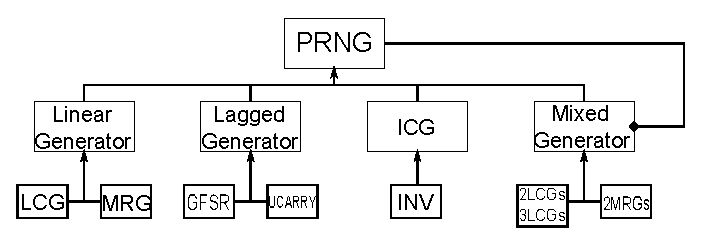
\includegraphics[width=3.5in]{TYPEPRNG.eps}
\DeclareGraphicsExtensions.
\caption{Ontological class hierarchy of PRNGs}
\label{Ontological class hierarchy of RNGs}
\end{figure}
\label{The generation of pseudorandom sequence}

\subsection{Blum Blum Shub}
The Blum Blum Shub generator~\cite{BBS} (usually denoted by BBS) takes the form:\\
$$x^0 \in \llbracket 1, m-1 \rrbracket$$
$$x^{n+1}=(x^n \times x^n) ~ mod~ m, ~~ y^{n+1} = x^{n+1}~ mod~ log(log(m)),$$  
where $m$ is the product of two prime numbers (these prime numbers  need to be congruent to $3$ modulus $4$), $x^n$ is an integer value, and it should be an integer that's co-prime to M. $y^n$ is the returned 
binary sequence. To be noticed, for its part, $log$ refers to the logarithm to base $2$.

\subsection{The logistic map}

The logistic map, given by:
\begin{center}
$x^{n+1}=\mu ~ x^{n}(1-x^{n})$, with $x^{0}\in(0,1)$, $\mu \in(3.99996,4]$,
\end{center}

\noindent where $x$ is a real number. Logistic map was originally introduced as a demographic model by Pierre Fran\c cois Verhulst in 1838. In 1947, Ulam and Von Neumann ~\cite{ulam1947} studied it as a PRNG. This essentially requires mapping the states of the system $\left(x^n\right)_{n \in \mathds{N}}$ to $\{0,1\}^\mathds{N}$. A simple way for turning $x^n$ to a discrete bit symbol $r$ is by using a threshold function as it is shown in Algo.\ref{logisticmap1}.
A second usual way to obtain an integer sequence from a real system is to chop off the leading bits after moving the decimal point of each $x$ to the right, as it is obtained in Algo.\ref{logisticmap2}.

\begin{algorithm}
\textbf{Input:} the internal state $x$ (a decimal number)\\
\textbf{Output:} $r$ (a 1-bit word)
\begin{algorithmic}[1]
\STATE$x\leftarrow{4x(1-x)}$
\IF{$x\textless0$}
{
\STATE$r\leftarrow0$;	
}
\ELSE
{
\STATE$r\leftarrow1$;	
}\ENDIF
\STATE return $r$\;
\medskip
\caption{An arbitrary round of logistic map 1}
\label{logisticmap1}
\end{algorithmic}
\end{algorithm}

\begin{algorithm}
\textbf{Input:} the internal state $x$ (a decimal number)\\
\textbf{Output:} $r$ (an integer)
\begin{algorithmic}[1]
\STATE$x\leftarrow{4x(1-x)}$
\STATE$r\leftarrow{\lfloor10000000x\rfloor}$
\STATE return $r$\;
\medskip
\caption{An arbitrary round of logistic map 2}
\label{logisticmap2}
\end{algorithmic}
\end{algorithm}

\subsection{LCG}
This PRNG implements either the simple or the combined linear congruency generator (LCGs). The simple LCG is defined by the recurrence:
\begin{equation}
x^n = (ax^{n-1} + c)~mod~m
\label{LCG}
\end{equation}
where $a$, $c$, and $x^0$ must be non-negative and less than $m$~\cite{Lecuyer2009} integers. In what follows, 2LCGs and 3LCGs refer as two (resp. three) combinations of such LCGs.
For further details, see~\cite{combined_lcg}.

\subsection{MRG}
This module implements multiple recursive generators (MRGs), based on a linear recurrence of order integer $k$, modulo $m$~\cite{Lecuyer2009}:
\begin{equation}
x^n = (a^1x^{n-1}+~...~+a^kx^{n-k})~mod~m
\label{MRG}
\end{equation}
Combination of two MRGs (referred as 2MRGs) is also used in this chapter.

\subsection{UCARRY}
Generators based on linear recurrences with carry are implemented in this module. This includes the add-with-carry (AWC) generator, based on the recurrence:
\begin{equation}
\label{AWC}
\begin{array}{l}
x^n = (x^{n-r} + x^{n-s} + c^{n-1})~mod~m, \\
c^n= (x^{n-r} + x^{n-s} + c^{n-1}) / m, \end{array}\end{equation}
with output: $x^i/m$. The $k$ initial values $(x^0,... ,x^{k-1})$ is firstly set with random integers.
the $k = max\{r, s\}$ (the bigger one assigned to $k$), and $c$ contains $c^0$. Restrictions: $0 < s, 0 < r, r\neq s$ and $c = 0 or 1$.

The SWB generator, having the recurrence:
\begin{equation}
\label{SWB}
\begin{array}{l}
x^n = (x^{n-r} - x^{n-s} - c^{n-1})~mod~m, \\
c^n=\left\{
\begin{array}{l}
1 ~~~~~\text{if}~ (x^{i-r} - x^{i-s} - c^{i-1})<0\\
0 ~~~~~\text{else},\end{array} \right. \end{array}\end{equation}
with output is $x^i/m$. The vector $S[0..(k-1)]$ contains
the $k$ initial values $(x^0,... x^{k-1})$, where $k = max\{r, s\}$, and $c$ contains $c0$. Restrictions : $0 < s,0 < r, r 6= s$ and $c = 0$ or $1$.
And the SWC generator designed by R. Couture, which is based on the following recurrence:
\begin{equation}
\label{SWC}
\begin{array}{l}
x^n = (a^1x^{n-1} \oplus ~...~ \oplus a^rx^{n-r} \oplus c^{n-1}) ~ mod ~ 2^w, \\
c^n = (a^1x^{n-1} \oplus ~...~ \oplus a^rx^{n-r} \oplus c^{n-1}) ~ / ~ 2^w. \end{array}\end{equation}
with output is $x^i/2^w$. The vector $(x^n,...x^{n-r+1}, c^n)$ is the state of the generator. The array $A[0..h-1]$ contains the polynomials $a^1,...,a^r$. Each even element stands for a polynomial number and the next
element stands for the corresponding nonzero coefficient number of that polynomial. The vector
$S[0..r-1]$ gives the initial values of $(x^0,...,x^{r-1})$ and $c$ is the initial carry. Restrictions: $0 < r,$
and $w \leq 32$.

\subsection{GFSR}
This module implements the generalized feedback shift register (GFSR) generator, that is:
\begin{equation}
x^n = x^{n-r} \oplus x^{n-k}
\label{GFSR}
\end{equation}
Where the $x$ sequence are initial with some random positive integers, $n>k$ and $n>r$.

\subsection{INV}
Finally, this module implements the nonlinear inversive generator, as defined in~\cite{Lecuyer2009}, which is:

\begin{equation}
\label{INV}
\begin{array}{l}
x^n=\left\{
\begin{array}{ll}
(a^1 + a^2 / z^{n-1})~mod~m & \text{if}~ z^{n-1} \neq 0 \\
a^1 & \text{if}~  z^{n-1} = 0 .\end{array} \right. \end{array}\end{equation}

The generator computes $z$ via the modified Euclid algorithm (see \cite{Lecuyer2009}). If $m$ is prime and if $p(x) = x^2 -a^1 x -a^2$ is a primitive polynomial modulo $m$, then the generator has maximal period $m$. Restrictions: $0 \leq z^0 < m, 0 < a^1 < m$ and $0 < a^2 < m$. Furthermore, $m$ must be a prime number, preferably large.


\subsection{XORshift}
\label{XORshift}

XORshift is a category of very fast PRNGs designed by George Marsaglia~\cite{Marsaglia2003}. It repeatedly uses the transform of \emph{exclusive or} (XOR) on a number with a bit shifted version of it. The state of a XORshift generator is a vector of bits. At each step, the next state is obtained by applying a given number of XORshift operations to $w$-bit blocks in the current state, where $w = 32$ or $64$. A XORshift operation is defined as follows. Replace the $w$-bit block by a bitwise XOR of the original block, with a shifted copy of itself by $a$ positions either to the right or to the left, where $ 0 < a < w$. This Algo.\ref{XORshift} is an example for $32$-bit XORshift, it has a period of $2^{32}-1=4.29\times10^9$.


\begin{algorithm}
\textbf{Input:} the internal state $z$ (a 32-bits word)\\
\textbf{Output:} $y$ (a 32-bits word)
\begin{algorithmic}[1]

\STATE$z\leftarrow{z\oplus{(z\ll13)}}$;
\STATE$z\leftarrow{z\oplus{(z\gg17)}}$;
\STATE$z\leftarrow{z\oplus{(z\ll5)}}$;
\STATE$y\leftarrow{z}$;
\STATE return $y$\;
\medskip
\caption{An arbitrary round of XORshift algorithm}
\label{XORshift}
\end{algorithmic}
\end{algorithm}

\subsection{ISAAC}
ISAAC is an array-based PRNG and a stream cipher designed by Robert Jenkins (1996) to be cryptographically secure~\cite{Jenkins1996}. The name is an acronym for Indirection, Shift, Accumulate, Add, and Count. The ISAAC algorithm has similarities with RC4~\cite{citeulike:3805944}. It uses an array of 256 32-bit integers as the internal state, writes the results to another 256-integer array, from which they are read one at a time until empty, at which point they are recomputed. Since it only takes about 19 32-bit operations for each 32-bit output word, it is extremely fast on 32-bit computers.

We give the key-stream procedure of ISAAC in Algo.\ref{ISAAC}. The internal state is $x$, the output array is $r$, and the inputs $32$-bit words $a$, $b$, and $c$ are those computed in the previous round. Normally $a$, $b$, $c$, and the array $r$ are initialized with some random sequences.% So we need the initial values of a,b, and c. Yes.
The value $f(a,i)$ in Algo.\ref{ISAAC} is a 32-bit word, defined for all $a$ and $i\in\{0,\dots,255\}$ as:

\begin{equation}
f(a,i) = \left\{\begin{array}{ll}
a\ll13 & \text{if } i~mod~4\equiv0 , \\
a\gg6 & \text{if } i~mod~4\equiv1 , \\
a\ll2 & \text{if } i~mod~4\equiv2, \\
a\gg16 & \text{if } i~mod~4\equiv3. \\
\end{array}
\right.
\end{equation}

\begin{algorithm}
\textbf{Input:} $a$, $b$, $c$, and the internal state $x$, they are $32$-bit words\\
\textbf{Output:} an array $r$ of 256 32-bit words
\begin{algorithmic}[1]
\STATE$c\leftarrow{c+1}$;
\STATE$b\leftarrow{b+c}$;
\WHILE{$i=0,\dots,255$}
\STATE$s\leftarrow{x_i}$;
\STATE$a\leftarrow{f(a,i)+x_{(i+128)~mod~256}}$;
\STATE$x_i\leftarrow{a+b+x_{(x\gg2)~mod~256}}$;
\STATE$r_i\leftarrow{s+x_{(x_i\gg10)~mod~256}}$;
\STATE$b\leftarrow{r_i}$;
\ENDWHILE
\STATE return $r$\;
\medskip
\caption{An arbitrary round of ISAAC algorithm}
\label{ISAAC}
\end{algorithmic}
\end{algorithm}





\section{CIPRNG, version 1~\cite{wang2009}}
\label{Version 1 CI algorithms and examples}
\subsection{Chaotic iterations as PRNG}
\label{subsec Chaotic iterations as PRNG}
This first proposed version of a generator based on chaotic iterations, 
denoted by CI version 1 (PRNG1,PRNG2) (PRNG1 and PRNG2 are the generators produce positive integer), is designed by the following process~\cite{wang2009}. 

Let $\mathsf{N} \in \mathds{N}^*, \mathsf{N} \geqslant 2$. Some chaotic iterations are fulfilled to generate a sequence $\left(x^n\right)_{n\in\mathds{N}} \in \left(\mathds{B}^\mathsf{N}\right)^\mathds{N}$ of Boolean vectors: the successive states of the iterated system. Some of these vectors are randomly extracted and their components constitute our pseudorandom bit flow.
\begin{algorithm}
\textbf{Input:} the internal state $x$ (an array of $\mathsf{N}$ 1-bit words)\\
\textbf{Output:} an array $r$ of $\mathsf{N}$ 1-bit words
\begin{algorithmic}[1]

\STATE$a\leftarrow{PRNG1()}$;
\STATE$m\leftarrow{a~mod~2+k}$;
\WHILE{$i=0,\dots,m$}
\STATE$b\leftarrow{PRNG2()}$;
\STATE$S\leftarrow{b~mod~\mathsf{N}}$;
\STATE$x_S\leftarrow{ \overline{x_S}}$;
\ENDWHILE
\STATE$r\leftarrow{x}$;
\STATE return $r$;
\medskip
\caption{An arbitrary round of the CI generator Version 1}
\label{Chaotic iteration}
\end{algorithmic}
\end{algorithm}

Chaotic iterations are realized as follows. Initial state $x^0 \in \mathds{B}^\mathsf{N}$ is a Boolean vector taken as a seed and strategy $\left(S^n\right)_{n\in\mathds{N}}\in \llbracket 1, \mathsf{N} \rrbracket^\mathds{N}$ is a sequence produced by PRNG2. Lastly, iterate function $f$ is the vectorial Boolean negation
$$f_0:(x_1,...,x_\mathsf{N}) \in \mathds{B}^\mathsf{N} \longmapsto (\overline{x_1},...,\overline{x_\mathsf{N}}) \in \mathds{B}^\mathsf{N}.$$
To sum up, at each iteration only $S^i$-th component of state $X^n$ is updated, as follows
\begin{equation}
x_i^n = \left\{\begin{array}{ll}x_i^{n-1} & \text{if } i \neq S^i, \\ \\ \overline{x_i^{n-1}} & \text{if } i = S^i. \\\end{array}\right.
\end{equation}

Finally, let $\mathcal{M}$ be a finite subset of $\mathds{N}^*$. Some $x^n$ are selected by a sequence $m^n$ as the pseudorandom bit sequence of our generator, $(m^n)_{n \in \mathds{N}} \in \mathcal{M}^\mathds{N}$ . So, the generator returns the following values: the components of $x^{m^0}$, followed by the components of $x^{m^0+m^1}$, followed by the components of $x^{m^0+m^1+m^2}$, \emph{etc.} In other words, the generator returns the following bits:

$$x_1^{m_0}x_2^{m_0}x_3^{m_0}\hdots x_\mathsf{N}^{m_0}x_1^{m_0+m_1}x_2^{m_0+m_1}\hdots x_\mathsf{N}^{m_0+m_1} x_1^{m_0+m_1+m_2}x_2^{m_0+m_1+m_2}\hdots$$
%and its $k^{th}$ bit is equal to $$\displaystyle{x_{k+1 \text{ (mod }\mathsf{N}\text{)}}^{\sum_{i=0}^{\lfloor k/\mathsf{N} \rfloor}m_i}}.$$

\noindent or the following integers:$$x^{m_0}x^{m_0+m_1}x^{m_0+m_1+m_2}\hdots$$


\subsection{CIPRNG version 1: the algorithm}
The basic design procedure of the CI generator version 1 is summed up in Algo.\ref{Chaotic iteration}. The internal state is $x$, the output array is $r$. $a$ and $b$ are those computed by PRNG1 and PRNG2. Lastly, $k$ and $\mathsf{N}$ are constants and \linebreak $\mathcal{M}=\{$k, k+1$\}$ ($k\geqslant 3\mathsf{N}$ is recommended, see \cite{bibtexwangqianxue} for more information).


\section{The CIPRNG: Version 2 ~\cite{wbg10:ip}}
%\subsection{Presentation}
%The CI generator (generator based on chaotic iterations) is designed by the following process. First of all, some chaotic iterations have to be done to generate a sequence 
%$\left(x^n\right)_{n\in\mathds{N}} \in \left(\mathds{B}^\mathsf{N}\right)^\mathds{N}$ 
%($\mathsf{N} \in \mathds{N}^*, \mathsf{N} \geqslant 2$, $N$ is not necessarily equal to 32) 
%of Boolean vectors, which are the successive states of the iterated system. Some of these vectors 
%will be randomly extracted and our pseudorandom bit flow will be constituted by their components. 
%Such chaotic iterations are realized as follows. 
%Initial state $x^0 \in \mathds{B}^\mathsf{N}$ is a Boolean vector taken as a 
%seed (see Section~\ref{algo seed}) and chaotic strategy $\left(S^n\right)_{n\in\mathds{N}}\in 
%\llbracket 1, \mathsf{N} \rrbracket^\mathds{N}$ is
%an irregular decimation of a random number sequence (Section~\ref{Chaotic strategy}). The iterate function $f$ is
%the vectorial Boolean negation:
%$$f_0:(x_1,...,x_\mathsf{N}) \in \mathds{B}^\mathsf{N} \longmapsto 
%(\overline{x_1},...,\overline{x_\mathsf{N}}) \in \mathds{B}^\mathsf{N}.$$
%At each iteration, only the $S^i$-th component of state $x^n$ is updated, 
%as follows: $x_i^n = x_i^{n-1}$ if $i \neq S^i$, else $x_i^n = \overline{x_i^{n-1}}$.
%Finally, some $x^n$ are selected
%by a sequence $m^n$ as the pseudorandom bit sequence of our generator.
%$(m^n)_{n \in \mathds{N}} \in \mathcal{M}^\mathds{N}$ is computed from 
%a PRNG, such as XORshift sequence $(y^n)_{n \in \mathds{N}} \in \llbracket 0, 
%2^{32}-1 \rrbracket$ (see Section~\ref{algo m}). So, the
%generator returns the following values:\newline
%\begin{small}
%Bits:$$x_1^{m_0}x_2^{m_0}x_3^{m_0}\hdots x_\mathsf{N}^{m_0}x_1^{m_0+m_1}x_2^{m_0+m_1}\hdots x_\mathsf{N}^{m_0+m_1} x_1^{m_0+m_1+m_2}\hdots$$
%or States:$$x^{m_0}x^{m_0+m_1}x^{m_0+m_1+m_2}\hdots$$
%\end{small}
%
%
%\subsection{The seed}
%\label{algo seed}
%The unpredictability of random sequences is established using
%a random seed that is obtained by a physical source like timings of keystrokes.
%Without the seed, the attacker must not be able to make any predictions about
%the output bits, even when all details of the generator are known~\cite{Turan2008}.
%
%The initial state of the system $x^0$ and the first term $y^0$ of the input PRNG are seeded either by
%the current time in seconds since the Epoch, or by a number that the user inputs.
%Different ways are possible. For example, let us denote by $t$ the decimal part of the current
%time. So $x^0$ can be $t \text{ (mod $2^N$)}$ written in binary digits and $y^0 = t$.
After the proof of concept of CIPRNG version 1, a second version of generator based on chaotic iterations has been introduced in \cite{wbg10:ip}.
\subsection{Defining the sequence $m^n$ }
\label{algo m}
The inputed PRNGs for CIPRNG version 2 (PRNG1, PRNG2) are the same as version 1. The basic idea was to prevent from changing a bit twice between two outputs, reducing by doing so the generation time. 
To do so, a sequence $(m^n)$ must be introduced, which defines the number 
of bits to change between two outputs.
The output of the sequence PRNG1 is uniform in $\llbracket 0, 2^{32}-1 \rrbracket$. However, we do not want the output of $(m^n)$ to be uniform in $\llbracket 0, N \rrbracket$, because in this case, the returns of our generator will not be uniform in $\llbracket 0, 2^{N}-1 \rrbracket$, as it is illustrated in the following example. Let us suppose that $x^0=(0,0,0)$. Then $m^0 \in \llbracket 0, 3 \rrbracket$. 
\begin{itemize}
\item If $m^0=0$, then no bit will change between the first and the second output of our CI PRNG Version 2. Thus $x^1 = (0,0,0)$.
\item If $m^0=1$, then exactly one bit will change, which leads to three possible values for $x^1$, namely $(1,0,0)$, $(0,1,0)$, and $(0,0,1)$.
\item \emph{etc.}
\end{itemize}
Each value in $\llbracket 0, 2^3-1 \rrbracket$ must be returned with the same frequency, then the values $(0,0,0)$, $(1,0,0)$, $(0,1,0)$, and $(0,0,1)$ must occur for $x^1$ with the same probability. Finally we see that, in this example, $m^0=1$ must be three times more probable than $m^0=0$.
This leads to the following general definition for the probability of $m=i$:
\begin{equation}
P(m^n=i)=\frac{C^i_N}{2^N}
\end{equation}

Then, here is an example for the $(m^n)$ sequence definition using a selector function $g_1$, where $y^n$ is the product of PRNG1:
\begin{equation}
\label{v2_g1}
m^n = g_1(y^n)=
\left\{
\begin{array}{l}
0 \text{ if }0 \leqslant\frac{y^n}{2^{32}}<\frac{C^0_N}{2^N},\\
1 \text{ if }\frac{C^0_N}{2^N} \leqslant\frac{y^n}{2^{32}}<\sum_{i=0}^1\frac{C^i_N}{2^N},\\
2 \text{ if }\sum_{i=0}^1\frac{C^i_N}{2^N} \leqslant\frac{y^n}{2^{32}}<\sum_{i=0}^2\frac{C^i_N}{2^N},\\
\vdots~~~~~ ~~\vdots~~~ ~~~~\\
N \text{ if }\sum_{i=0}^{N-1}\frac{C^i_N}{2^N} \leqslant\frac{y^n}{2^{32}}<1.\\
\end{array}
\right.
\end{equation}

The CI PRNG Version 2 can use any reasonable function as selector like ~\cite{bibtexwangqianxue}:
\begin{equation}
\label{v2_g2}
m^n = g_2(y^n)=
\left\{
\begin{array}{l}
N \text{ if }0 \leqslant\frac{y^n}{2^{32}}<\frac{C^0_N}{2^N},\\
N-1 \text{ if }\frac{C^0_N}{2^N} \leqslant\frac{y^n}{2^{32}}<\sum_{i=0}^1\frac{C^i_N}{2^N},\\
N-2 \text{ if }\sum_{i=0}^1\frac{C^i_N}{2^N} \leqslant\frac{y^n}{2^{32}}<\sum_{i=0}^2\frac{C^i_N}{2^N},\\
\vdots~~~~~ ~~\vdots~~~ ~~~~\\
0 \text{ if }\sum_{i=0}^{N-1}\frac{C^i_N}{2^N} \leqslant\frac{y^n}{2^{32}}<1.\\
\end{array}
\right.
\end{equation}

In this thesis, $g_1()$ is the selector function unless noted otherwise. 


\subsection{strategy}
\label{Chaotic strategy}
The strategy $(S^k) \in \llbracket 1, N \rrbracket^\mathds{N}$ is generated using a second generator PRNG2's sequence $(b^k) \in \llbracket 1, N \rrbracket^\mathds{N}$ (see \cite{Bahi2000} for further details). The only difference between the sequences $S$ and $b$ is that some terms of $b$ are discarded, in such a way that $\forall k \in \mathds{N}, (S^{M^k}, S^{M^k+1}, \hdots, S^{M^{k+1}-1})$ does not contain any given integer twice, where $M^k = \sum_{i=0}^k m^i$. Therefore, no bit will change more than once between two successive outputs of this PRNG proposed in \cite{wbg10:ip}, increasing the speed of the former generator by doing so. $S$ is said to be ``an irregular decimation'' of $b$. This decimation can be obtained by the following process (see \cite{wbg10:ip}).

Let $(d^1,d^2,\dots,d^N)\in \{0,1\}^N$ be a mark sequence, such that whenever $\sum_{i=1}^N d^i = m^k$,
then $\forall i, d_i=0$ ($\forall k$, the sequence is reset when $d$ contains $m^k$ times the number 1). This mark sequence will control the PRNG2 sequence $b$ as follows:
\begin{itemize}
\item if $d^{b^j} \neq 1$, then $S^k=b^j$, $d^{b^j} = 1$, and $k = k+1$,
\item if $d^{b^j}=1$, then $b^j$ is discarded.
\end{itemize}
For example, if $b = 142\underline{2}334 1421\underline{1}\underline{2}\underline{2}34...$ and $m = 4341...$, then $S=1423~341~4123~4...$ However, if we do not use the mark sequence, then one position may change more than once and the balance property will not be checked, due to the fact that $\bar{\bar{x}}=x$. As an example, for $b$ and $m$ as in the previous example, $S=1422~334~1421~1...$ and $S=14~4~42~1...$ lead to the same output (because switching the same bit twice leads to the same state).

 
To check the balance property, a set of $500$
sequences are generated with and without decimation, each
sequence containing $10^6$ bits. Fig.\ref{nmark} shows the
percentages of differences between zeros and ones, and presents a better balance property for the sequences with decimation. This claim has been verified in the tests~\cite{wbg10:ip}. 

\begin{figure}
\centering
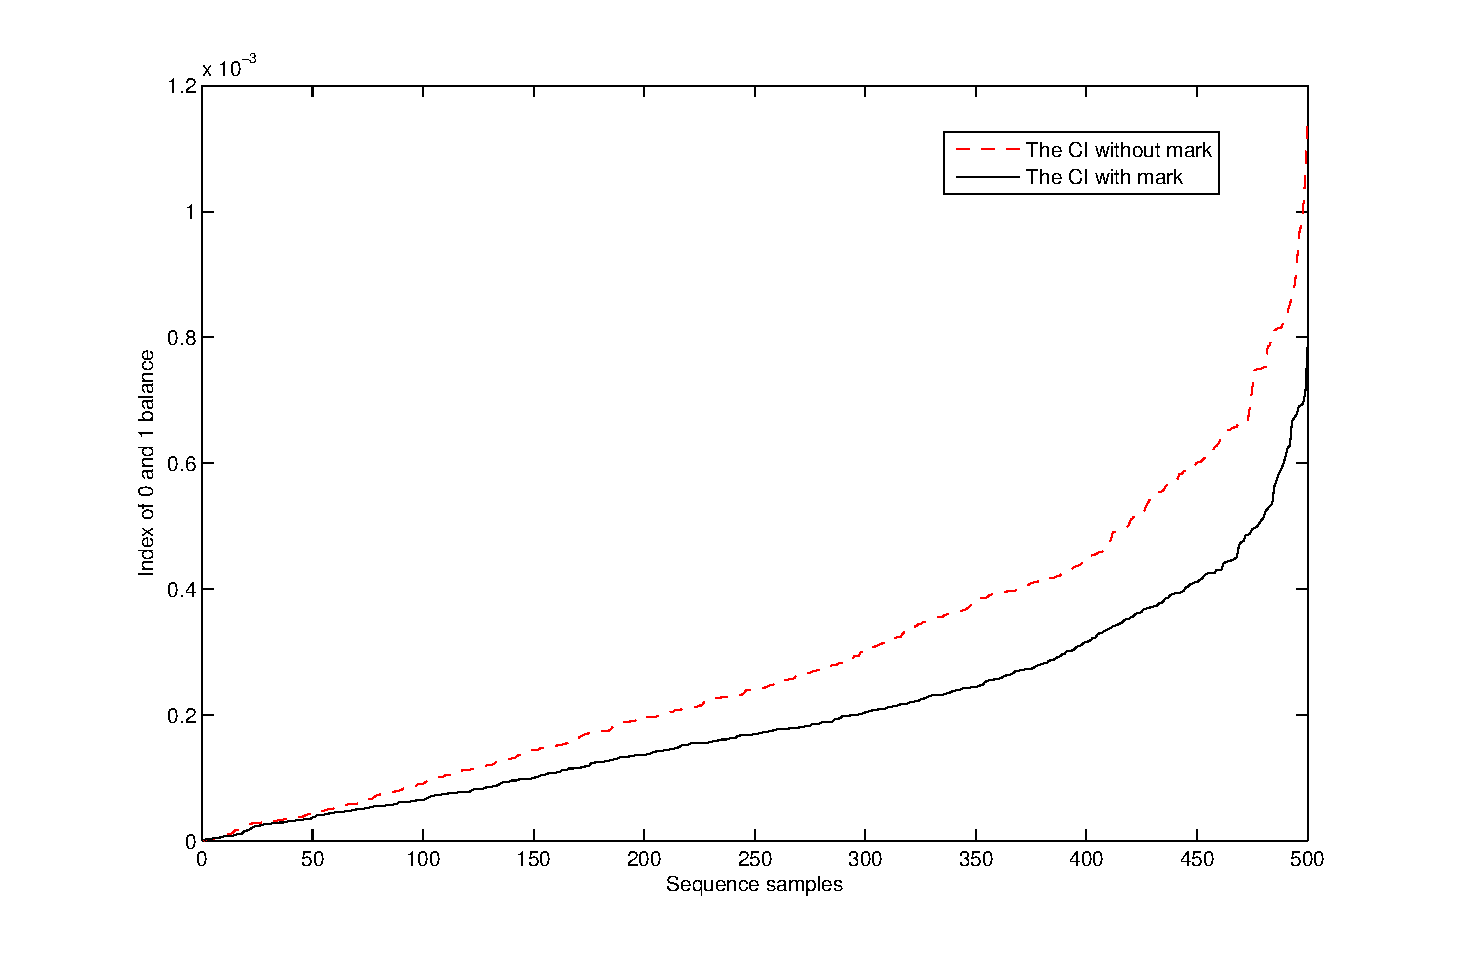
\includegraphics[width=15cm]{nmark.eps}
\DeclareGraphicsExtensions.
\caption{Balance property}
\label{nmark}
\end{figure}


\subsection{CIPRNG version 2: the algorithm}

The basic design procedure of the novel generator is summed up in Algo.\ref{Chaotic iteration1}.
The internal state is $x$, it is an integer of $N$ bits size. The output state is $r$. $a$ and $b$ are those computed by the two input
PRNGs. The value $g_1(a)$ is an integer, defined as in Eq.(\ref{v2_g1}). Lastly, $\mathsf{N}$ is a constant 
defined by the user.
\begin{algorithm}
\textbf{Input:} the internal state $x$ ($N$ bits)\\
\textbf{Output:} a state $r$ ($N$ bits)\\
\begin{algorithmic}[1]
\FOR{$i=0,\dots,N$}
{
\STATE$d_i\leftarrow{0}$\;
}
\ENDFOR
\STATE$a\leftarrow{PRNG1()}$\;
\STATE$m\leftarrow{f(a)}$\;
\STATE$k\leftarrow{m}$\;
\WHILE{$i=0,\dots,k$}

\STATE$b\leftarrow{PRNG2()~mod~N}$\;
\STATE$S\leftarrow{b}$\;
    \IF{$d_S=0$}
    {
\STATE      $x_S\leftarrow{ \overline{x_S}}$\;
\STATE      $d_S\leftarrow{1}$\;
    
    }
    \ELSIF{$d_S=1$}
    {
\STATE      $k\leftarrow{ k+1}$\;
    }\ENDIF
\ENDWHILE
$r\leftarrow{x}$\;
return $r$\;
\medskip
\caption{An arbitrary round of the CI generator Version 2}
\label{Chaotic iteration1}
\end{algorithmic}
\end{algorithm}

Compare to CI Version 1, this latter version provides better statistical performance and speed \cite{bfgw11:ij}.


\section{XOR CIPRNG}
Instead of updating only one cell at each iteration as the previous versions of
our CIPRNGs, we can try to choose a subset of components and to update them together. Such an attempt leads
to a kind of merger of the two random sequences. When the updating function is the vectorial 
negation, this algorithm can be rewritten as follows~\cite{DBLP:journals/corr/abs-1112-5239}:

\begin{equation}
\left\{
\begin{array}{l}
x^0 \in \llbracket 0, 2^\mathsf{N}-1 \rrbracket, S \in \llbracket 0, 2^\mathsf{N}-1 \rrbracket^\mathds{N} \\
d^n = S^n\\
\forall n \in \mathds{N}^*, x^n = x^{n-1} \oplus d^n,
\end{array}
\right.
\label{equation Oplus1}
\end{equation}

\noindent and this rewriting can be understood as follows. The $n^{th}$ term $S^n$ of the sequence $S$, 
which is an integer of $\mathsf{N}$ binary digits, presents
the list of cells to update in the state $x^n$ of the system (represented as an integer 
having $\mathsf{N}$ bits too). More precisely, the $k^{th}$
component of this state (a binary digit) changes if and only if the $k^{th}$ digit in the 
binary decomposition of $S^n$ is 1. This generator has been called XOR CIPRNG by
the AND team, which has introduced and studied it in\cite{DBLP:journals/corr/abs-1112-5239, bfg12a:ip}.

The single basic component presented in Eq.(\ref{equation Oplus1}) is of ordinary use as a 
good elementary brick in various PRNGs. It corresponds
to the discrete dynamical system in chaotic iterations.
Such XOR CIPRNG has inspired us to introduce a more general category of CIPRNGs, presented
in Chapter~\ref{CI dev}.
%As a comparison, the basic design procedure of the old generator 
%is recalled in Algorithm~\ref{Chaotic iteration2} ($a$ and $b$ are computed by two input PRNGs, 
%$\mathsf{N}$ and $c\geqslant 3\mathsf{N}$ are constants defined by the user). 
%See Subsection~\ref{Version 1 CI algorithms and examples} for further information.
%
%
%\begin{algorithm}
%\textbf{Input:} the internal state $x$ (an array of $\mathsf{N}$ 1-bit words)\\
%\textbf{Output:} an array $r$ of $\mathsf{N}$ 1-bit words
%\begin{algorithmic}[1]
%
%\STATE$a\leftarrow{PRNG1()}$;
%\STATE$m\leftarrow{a~mod~2+c}$;
%\WHILE{$i=0,\dots,m$}
%\STATE$b\leftarrow{PRNG2()}$;
%\STATE$S\leftarrow{b~mod~\mathsf{N}}$;
%\STATE$x_S\leftarrow{ \overline{x_S}}$;
%\ENDWHILE
%\STATE$r\leftarrow{x}$;
%\STATE return $r$;
%\medskip
%\caption{An arbitrary round of the old CI generator}
%\label{Chaotic iteration2}
%\end{algorithmic}
%\end{algorithm}
%

%\subsection{Illustrative Example of Version 2 CI (XORshift, XORshift)}
%
%In this example, $\mathsf{N} = 4$ is chosen for easy understanding and the input PRNG is XORshift PRNG. As stated before, the initial state of the system $x^0$ can be seeded by the decimal part $t$ of the current time. For example, if the current time in seconds since the Epoch is 1237632934.484088,
%so $t = 484088$, then $x^0 = t \text{ ($mod$ 16)}$ in binary digits, \emph{i.e.}, $x^0 = ( 0, 1, 0, 0)$.
%
%To compute $m$ sequence, Eq.(\ref{v2_g1}) can be adapted to this example as follows:
%\begin{equation}
%\label{m1 fuction}
%m^n=g_1(y^n)=
%\left\{
%\begin{array}{llccccc}
%0 & \text{ if }&0 &\leqslant&\frac{y^n}{2^{32}}&<&\frac{1}{16},\\
%1 & \text{ if }&\frac{1}{16} &\leqslant&\frac{y^n}{2^{32}}&<&\frac{5}{16} ,\\
%2 & \text{ if }&\frac{5}{16} &\leqslant&\frac{y^n}{2^{32}}&<&\frac{11}{16},\\
%3 & \text{ if }&\frac{11}{16} &\leqslant&\frac{y^n}{2^{32}}&<&\frac{15}{16},\\
%4 & \text{ if }&\frac{15}{16} &\leqslant&\frac{y^n}{2^{32}}&<&1,\\
%\end{array}
%\right.
%\end{equation}
%
%\noindent where $y$ is generated by XORshift seeded with the current time. 
%We can see that the probabilities of occurrences of $m=0$, $m=1$, $m=2$, $m=3$, $m=4$, 
%are $\frac{1}{16}$, $\frac{4}{16}$, $\frac{6}{16}$, $\frac{4}{16}$, $\frac{1}{16}$, respectively. 
%This $m$ determines what will be the next output $x$. For instance,
%\begin{itemize}
%\item If $m=0$, the following $x$ will be $( 0, 1, 0, 0)$.
%\item If $m=1$, the following $x$ can be $( 1, 1, 0, 0)$, $( 0, 0, 0, 0)$, $( 0, 1, 1, 0)$, or $( 0, 1, 0, 1)$.
%\item If $m=2$, the following $x$ can be $( 1, 0, 0, 0)$, $( 1, 1, 1, 0)$, $( 1, 1, 0, 1)$, $( 0, 0, 1, 0)$, $( 0, 0, 0, 1)$, or $( 0, 1, 1, 1)$.
%\item If $m=3$, the following $x$ can be $( 0, 0, 1, 1)$, $( 1, 1, 1, 1)$, $( 1, 0, 0, 1)$, or $( 1, 0, 1, 0)$.
%\item If $m=4$, the following $x$ will be $( 1, 0, 1, 1)$.
%\end{itemize}
%
%In this simulation, $m = 0, 4, 2, 2, 3, 4, 1, 1, 2, 3, 0, 1, 4,...$ Additionally, 
%$b$ is computed with a XORshift generator too, but with another seed. We have found 
%$b = 1, 4, 2, 2, 3, 3, 4, 1, 1, 4, 3, 2, 1,...$
%
%Chaotic iterations are made with initial state $x^0$, vectorial logical negation $f_0$, and
%strategy $S$. The result is presented in Tab.\ref{table application example}. Let us 
%recall that sequence $m$ gives the states $x^n$ to return, which are here $x^0, x^{0+4}, 
%x^{0+4+2}, \hdots$ So, in this example, the output of the generator is: 10100111101111110011... or 4,4,11,8,1...
%
%\begin{table*}[!t]
%%\renewcommand{\arraystretch}{1.3}
%\centering
%\begin{tabular}{|c|c@{}c|c@{}c@{}c@{}c@{}c@{}c|c@{}c@{}c|c@{}c@{}c@{}c|}
%\hline
%$m$ &0 & &4 & & & & & &2& &&2&&  &  \\ \hline
%$k$ &0 & &4 & & &$+1$ & & &2& &&2&$+1$&  &  \\ \hline
%$b$  &  & &1 &4&2&\underline{2}       &3& &3&4&&1&\underline{1}      &4&\\ \hline
%$d$  &r  & &r~$\left(\begin{array}{c}1\\0\\0\\0\end{array}\right)$ & $\left(\begin{array}{c}1\\0\\0\\1\end{array}\right)$ & $\left(\begin{array}{c}1\\1\\0\\1\end{array}\right)$ & & $\left(\begin{array}{c}1\\1\\1\\1\end{array}\right)$ && r~$\left(\begin{array}{c}0\\0\\1\\0\end{array}\right)$ &$\left(\begin{array}{c}0\\0\\1\\1\end{array}\right)$ &&r~$\left(\begin{array}{c}1\\0\\0\\0\end{array}\right)$ & &$\left(\begin{array}{c}1\\0\\0\\1\end{array}\right)$  &  \\ \hline
%$S$  &  & &1 &4&2&        &3& &3&4&&1& &4 &  \\ \hline
%$x^{0}$ &  &$x^{0}$ & & &  
%&  & &$x^{4}$ & & &   
%$x^{6}$& & &&$x^{8}$  \\
%%1ere ligne
%0 & &0 &$\xrightarrow{1} 1$ & &
% & &   &1   & & &
%1 &$\xrightarrow{1} 0$ & & & 0\\
%%2eme ligne
%1 &  &1 &   &   &
%$\xrightarrow{2} 0$ & & &0 & & &
%0 & &  &&0\\
%%3eme ligne
%0 & &0 & & &
% & &$\xrightarrow{3} 1$ &1 &$\xrightarrow{3} 0$ & &
%0 &   & & &0  \\
%% 4eme ligne
%0 & &0  & &$\xrightarrow{4} 1$ &
% & & &1 & &$\xrightarrow{4} 0$ &
%0 & & &$\xrightarrow{4} 1$&1 \\
%\hline
%\end{tabular}\\
%\vspace{0.5cm}
%Binary Output: $x_1^{0}x_2^{0}x_3^{0}x_4^{0}x_1^{4}x_2^{4}x_3^{4}x_4^{4}x_1^{6}x_2^{6}... = 0100101110000001...$\\
%Integer Output:
%$x^{0},x^{4},x^{6},x^{8}... = 4,11,8,1...$
%\caption{Example of Version 2 CI(XORshift,XORshift) generation}
%\label{table application example}
%\end{table*}

\chapter{Investigating the Design of new CIPRNGs}
\label{CI dev}
\minitoc

In this chapter, we deepened the capacity for the CIPRNG post-treatment method 
to improve the statistics of large varieties of pseudorandom generators. Then some formerly proposed researches on CIPRNGs versions 1 and 2 are deepened, the designs of our two brand new versions of discrete chaotic iterations based pseudorandom number generators are proposed and discussed. Detail operations of the proposed approach are described in this chapter, while their performance and  comparative studies will be presented in the next one. Finally, FPGA implementations of
some generators are proposed. 

The works presented in this chapter have been formerly published in \cite{submit2,bfg12a:ip} and submitted in \cite{submit1, submit3}.

\section{An Optimization Technique on Pseudorandom Generators Based on Chaotic Iterations}
In this section, the behavior of the CIPRNG versions previously presented 
are carried out systematically regarding 
the statistics improvement of the inputted generators.

\subsection{The tested PRNGs}

CIPRNGs versions 1, 2, and XOR are experimented here on various inputted PRNGs,
some of them being more or less defective.
Since different biased generators can possibly have their own side effects when inputted into our mixed generators, it is normal to enlarge the set of tested inputted PRNGs, to determine if the observed improvement still remains.
We will thus show in this chapter that the intended statistical improvement is really effective for all of these most famous generators (these works have been
formerly published in~\cite{bfg12a:ip}).

Knowing that there is no universal generator, it is strongly recommended to test a stochastic application with a large set of different PRNGs~\cite{DavidRC2003643}. Such generators should cover the four major classes: linear generators, lagged generators, inversive generators, and mix generators described in Chapter~\ref{Review of works}. In this section, the ten PRNGs presented in Chapter~\ref{Review of works} have been considered for experiments:
\begin{itemize}
\item LCG, MRG for linear congruential PRNGs; 
\item AWC, SWB, SWC, and GFSR for Lagged ones;
\item INV from type ICG;
\item lastly, 2LCG, 3LCG, and 2MRG to study Mixed PRNGs. 
\end{itemize}
%For instance, coupling inversive generators with linear congruential generators (LCGs) can be very interesting,
%because their internal structure and correlation behavior strongly differ from what LCGs produce.
%Since these generators have revealed several issues, some scientists refrain from using them.
%In what follows, the chaotic iteration applying finite source PRNG leading to noticeable improvements observed by statistical tests.
%A theoretical proof for the randomness of a generator is impossible to give, therefore statistical inference based on observed sample sequences produced by the generator seems to be the best option.
%Considering the properties of binary random sequences, various statistical tests can be designed to evaluate the assertion that the sequence is generated by a perfectly random source. 
We have performed some statistical tests on these generators, showing that 
they reveal several issues. Then we have compared these results with 
the ones obtained after a chaotic iterations post-treatment.
The tests studied here are the NIST suite~\cite{ANDREW2008} and DieHARD battery of tests~\cite{Marsaglia1996}.

\subsection{Results of PRNGs}
\label{Results and discussion}

\begin{sidewaystable}
\caption{NIST and DieHARD tests suite passing rates for PRNGs without CI}
\label{NIST and DieHARD tests suite passing rate the for PRNGs without CI}
\centering
\begin{tabular}{|l||c|c|c|c|c|c|c|c|c|c|}
    \hline\hline
Types of PRNGs & \multicolumn{2}{c|}{Linear PRNGs} & \multicolumn{4}{c|}{Lagged PRNGs} & \multicolumn{1}{c|}{ICG PRNGs} & \multicolumn{3}{c|}{Mixed PRNGs}\\ \hline
\backslashbox{\textbf{$Tests$}} {\textbf{$PRNG$}} & LCG& MRG& AWC & SWB  & SWC & GFSR & INV & LCG2& LCG3& MRG2 \\ \hline
NIST & 11/15 & 14/15 &\textbf{15/15} & \textbf{15/15}   & 14/15 & 14/15  & 14/15 & 14/15& 14/15& 14/15 \\ \hline
DieHARD & 16/18 & 16/18 & 15/18 & 16/18 & \textbf{18/18} & 16/18 & 16/18 & 16/18& 16/18& 16/18\\ \hline
\end{tabular}
\end{sidewaystable}



Table~\ref{NIST and DieHARD tests suite passing rate the for PRNGs without CI} shows the results on the batteries recalled in a
previous chapter, indicating that almost all the PRNGs considered here cannot pass all their embedding tests. In other words, the statistical quality of these PRNGs cannot fulfill the up-to-date standards presented previously. We will show that the CIPRNG can solve this issue.

To illustrate the effects of this CIPRNG in detail, experiments will be divided in three parts:
\begin{enumerate}
  \item \textbf{Single CIPRNG}: The PRNGs involved into the chaotic iterations computing are of the same category.
  \item \textbf{Mixed XOR CIPRNG}: Two different types of generators are xored, and then inputted to the XOR CIPRNG process.
  \item \textbf{Multiple XOR CIPRNG}: Various successive terms of the inputted generator are xored together, and the result is passed to our XOR CIPRNG.
%The generator is obtained by repeating the composition of the iteration function as follows: $x^0\in \mathds{B}^{\mathsf{N}}$, and $\forall n\in \mathds{N}^{\ast },\forall i\in \llbracket1;\mathsf{N}\rrbracket,$
%\begin{equation}
%\begin{array}{l}
%x_i^n=\left\{
%\begin{array}{l}
%x_i^{n-1}~~~~~\text{if}~S^n\neq i \\
%\forall j\in \llbracket1;\mathsf{m}\rrbracket,f^m(x^{n-1})_{S^{nm+j}}~\text{if}~S^{nm+j}=i.\end{array} \right. \end{array}
%\end{equation}
%$m$ is called the \emph{functional power}.
\end{enumerate}

We have performed statistical analysis on each of the aforementioned CIPRNGs.
The results are reproduced in Tab.~\ref{NIST and DieHARD tests suite passing rate the for PRNGs without CI} and \ref{NIST and DieHARD tests suite passing rate the for single CIPRNGs}.
The scores written in boldface indicate that all the tests have been passed successfully, whereas an asterisk ``*'' means that the considered passing rate has been improved.
\subsection{Tests Based on The Single CIPRNG}

\begin{sidewaystable}
\renewcommand{\arraystretch}{1.3}
\caption{NIST and DieHARD tests suite passing rates for PRNGs with CI}
\label{NIST and DieHARD tests suite passing rate the for single CIPRNGs}
\centering
  \begin{tabular}{|l||c|c|c|c|c|c|c|c|c|c|c|c|}
    \hline
Types of PRNGs & \multicolumn{2}{c|}{Linear PRNGs} & \multicolumn{4}{c|}{Lagged PRNGs} & \multicolumn{1}{c|}{ICG PRNGs} & \multicolumn{3}{c|}{Mixed PRNGs}\\ \hline
\backslashbox{\textbf{$Tests$}} {\textbf{$Single~CIPRNG$}} & LCG  & MRG & AWC & SWB & SWC & GFSR & INV& LCG2 & LCG3& MRG2 \\ \hline\hline
Version 1 CIPRNG\\ \hline \hline
NIST & \textbf{15/15} *  & \textbf{15/15} * & \textbf{15/15}   & \textbf{15/15}   & \textbf{15/15} * & \textbf{15/15} * & \textbf{15/15} *& \textbf{15/15} * & \textbf{15/15} * & \textbf{15/15} \\ \hline
DieHARD & \textbf{18/18} *  & \textbf{18/18} * & \textbf{18/18} *  & \textbf{18/18} *  & \textbf{18/18}  & \textbf{18/18} * & \textbf{18/18} *& \textbf{18/18} * & \textbf{18/18} *& \textbf{18/18} * \\ \hline
Version 2 CIPRNG\\ \hline \hline
NIST & \textbf{15/15} *  & \textbf{15/15} * & \textbf{15/15}   & \textbf{15/15}  & \textbf{15/15} * & \textbf{15/15} * & \textbf{15/15} *& \textbf{15/15} * & \textbf{15/15} * & \textbf{15/15} \\ \hline
DieHARD & \textbf{18/18} *  & \textbf{18/18} * & \textbf{18/18} * & \textbf{18/18} * & \textbf{18/18}  & \textbf{18/18} * & \textbf{18/18} * & \textbf{18/18} * & \textbf{18/18} *& \textbf{18/18} *\\ \hline
XOR CIPRNG\\ \hline\hline
NIST & 14/15*& \textbf{15/15} *   & \textbf{15/15}   & \textbf{15/15}   & 14/15 & \textbf{15/15} * & 14/15& \textbf{15/15} * & \textbf{15/15} *& \textbf{15/15}  \\ \hline
DieHARD & 16/18 & 16/18 & 17/18* & \textbf{18/18} * & \textbf{18/18}  & \textbf{18/18} * & 16/18 & 16/18 & 16/18& 16/18\\ \hline
\end{tabular}
\end{sidewaystable}

The statistical tests results of the PRNGs using the single CIPRNG method are given in Tab.~\ref{NIST and DieHARD tests suite passing rate the for single CIPRNGs}.
We can observe that, except for the XOR CIPRNG, all of the CIPRNGs have passed the 15 tests of the NIST battery and the 18 tests of the DieHARD one.
Moreover, considering these scores, we can deduce that both the single Version 1 CIPRNG and the single Version 2 CIPRNG are relatively steadier than the single XOR CIPRNG approach, when applying them to different PRNGs.
However, the XOR CIPRNG is obviously the fastest approach to generate a CI random sequence, and it still improves the statistical properties relative to each generator taken alone, although the test values are not as good as desired.

Therefore, all of these three ways are interesting, for different reasons, in the production of pseudorandom numbers and,
on the whole, the single CIPRNG method can be considered to adapt to or improve all kinds of PRNGs.

To have a realization of the XOR CIPRNG that can pass all the tests embedded into the NIST battery, we will now investigate the ``Mixed XOR CIPRNG'' and the ``Multiple XOR
CIPRNG'' variations of the XOR post-treatment in the following sections.



\subsection{Tests Based on The Mixed XOR CIPRNG}

We have considered here the same inputted generators than in the previous section.
These inputted couples $(PRNG_1,PRNG_2)$ of PRNGs are used in the Mixed approach as follows:
\begin{equation}
\left\{
\begin{array}{l}
x^0 \in \llbracket 0, 2^\mathsf{N}-1 \rrbracket \\
\forall n \in \mathds{N}^*, x^n = x^{n-1} \oplus PRNG_1\oplus PRNG_2,
\end{array}
\right.
\label{equation Oplus}
\end{equation}

We have checked that the generators used previously together with a XOR CIPRNG post-treatment can now pass more tests.
The main reason of this success is that the Mixed XOR CIPRNG should has a longer period, that still remains to be computed.
%Indeed, let $n_{P}$ be the period of a PRNG $P$, then the period deduced from the single XOR CIPRNG approach is obviously equal to:
%\begin{equation}
%n_{SXORCI}=
%\left\{
%\begin{array}{ll}
%n_{P}&\text{if~}x^0=x^{n_{P}}\\
%2n_{P}&\text{if~}x^0\neq x^{n_{P}}.\\
%\end{array}
%\right.
%\label{equation Oplus}
%\end{equation}

%Let us now denote by $n_{P1}$ and $n_{P2}$ the periods of respectively the $PRNG_1$ and $PRNG_2$ generators, then the period of the Mixed XOR CIPRNG will be:
%\begin{equation}
%n_{XXORCI}=
%\left\{
%\begin{array}{ll}
%LCM(n_{P1},n_{P2})&\text{if~}x^0=x^{LCM(n_{P1},n_{P2})}\\
%2LCM(n_{P1},n_{P2})&\text{if~}x^0\neq x^{LCM(n_{P1},n_{P2})}.\\
%\end{array}
%\right.
%\label{equation Oplus}
%\end{equation}

In Tab.~\ref{DieHARD fail mixex CIPRNG}, we only show the results for the Mixed XOR CIPRNGs that cannot pass all DieHARD suites (the NIST tests are all passed). It demonstrates that Mixed XOR CIPRNG involving LCG, MRG, LCG2, LCG3, MRG2, or INV cannot pass the two following tests, namely the ``Matrix Rank 32x32'' and the ``COUNT-THE-1's'' tests contained into the DieHARD battery. Let us recall their definitions:

\begin{itemize}
 \item \textbf{Matrix Rank 32x32.} A random 32x32 binary matrix is formed, each row having a 32-bit random vector. Its rank is an integer that ranges from 0 to 32. Ranks less than 29 must be rare, and their occurences must be pooled with those of rank 29. To achieve the test, ranks of 40,000 such random matrices are obtained, and a chisquare test is performed on counts for ranks 32,31,30 and for ranks $\leq29$.

 \item \textbf{COUNT-THE-1's TEST} Consider the file under test as a stream of bytes (four per  2 bit integer).  Each byte can contain from 0 to 8 1's, with probabilities 1,8,28,56,70,56,28,8,1 over 256.  Now let the stream of bytes provide a string of overlapping  5-letter words, each ``letter'' taking values A,B,C,D,E. The letters are determined by the number of 1's in a byte: 0,1, or 2 yield A, 3 yields B, 4 yields C, 5 yields D and 6,7, or 8 yield E. Thus we have a monkey at a typewriter hitting five keys with various probabilities (37,56,70,56,37 over 256).  There are $5^5$ possible 5-letter words, and from a string of 256,000 (over-lapping) 5-letter words, counts are made on the frequencies for each word.   The quadratic form in the weak inverse of the covariance matrix of the cell counts provides a chisquare test: Q5-Q4, the difference of the naive Pearson sums of $(OBS-EXP)^2/EXP$ on counts for 5- and 4-letter cell counts.
\end{itemize}

The reason of these fails is that the output of LCG, LCG2, LCG3, MRG, and MRG2 under experiments are in 31-bit. Compared to the single XOR CIPRNG, to use
two PRNGs of different kind in a Mixed XOR CIPRNG seems more efficient in improving random number quality (mixed XOR can pass 100\% of the NIST, whereas single cannot do it).

\begin{table*}
\renewcommand{\arraystretch}{1.3}
\caption{Scores of Mixed XOR CIPRNGs when considering the DieHARD battery}
\label{DieHARD fail mixex CIPRNG}
\centering
  \begin{tabular}{|l||c|c|c|c|c|c|}
    \hline
\backslashbox{\textbf{$PRNG_1$}} {\textbf{$PRNG_2$}} & LCG & MRG & INV & LCG2 & LCG3 & MRG2 \\ \hline\hline
LCG  &\backslashbox{} {} &16/18&16/18 &16/18 &16/18 &16/18\\ \hline
MRG &16/18 &\backslashbox{} {} &16/18&16/18 &16/18  &16/18\\ \hline
INV &16/18 &16/18&\backslashbox{} {} &16/18 &16/18&16/18    \\ \hline
LCG2  &16/18 &16/18 &16/18 &\backslashbox{} {}  &16/18&16/18\\ \hline
LCG3  &16/18 &16/18 &16/18&16/18&\backslashbox{} {} &16/18\\ \hline
MRG2 &16/18  &16/18 &16/18&16/18 &16/18 &\backslashbox{} {}  \\ \hline
\end{tabular}
\end{table*}

\subsection{Tests Based on The Multiple XOR CIPRNG}
\label{Tests based on Multiple XOR CIPRNG}

%Until now, the combination of at most two input PRNGs has been investigated.
We now regard the possibility to use various successive terms of a given 
deficient generator $S$ and to improve its statistics.
Such a desire leads to the Multiple XOR CIPRNG detailed
below: %One of the objectives of this natural approach is to illustrate
%the statistical improvement due to chaotic iterations post-treatment.

%For the CIPRNGs which have already pass both the NIST and DieHARD suites with 2 inputted PRNGs 
%(all the Old and Version 2 CIPRNGs, and some of the XOR CIPRNGs), it is not meaningful to consider 
%their adaption of this Multiple XOR CIPRNG method, hence only t
%The Multiple XOR CIPRNGs defined below will now be investigated investigated.
\begin{equation}
\left\{
\begin{array}{l}
x^0 \in \llbracket 0, 2^\mathsf{N}-1 \rrbracket, S \in \llbracket 0, 2^\mathsf{N}-1 \rrbracket^\mathds{N} \\
\forall n \in \mathds{N}^*, x^n = x^{n-1} \oplus S^{nm}\oplus S^{nm+1}\ldots \oplus S^{nm+m-1} ,
\end{array}
\right.
\label{equation Oplus}
\end{equation}
where $S$ stands for the inputted PRNG.
The question is now to determine the value of the threshold $m$ (the functional power) making 
the Multiple XOR CIPRNG being able to pass the whole NIST battery.
Such a question is answered in Tab.~\ref{threshold}, illustrating in a certain 
extend the progressive appearance of the effects of chaos.


\begin{table*}
\renewcommand{\arraystretch}{1.3}
\caption{Functional power $m$ making it possible to pass the whole NIST battery}
\label{threshold}
\centering
  \begin{tabular}{|l||c|c|c|c|c|c|c|c|}
    \hline
Inputted $PRNG$ & LCG & MRG & SWC & GFSR & INV& LCG2 & LCG3  & MRG2 \\ \hline\hline
Threshold  value $m$& 19 & 7  & 2& 1 & 11& 9& 3& 4\\ \hline\hline
\end{tabular}
\end{table*}

\subsection{Results Summary}

We can summarize the obtained results as follows.
\begin{enumerate}
\item The CIPRNG method is able to improve the statistical properties of a large variety of PRNGs.
\item Using different PRNGs in the CIPRNG approach is better than considering several instances of one unique PRNG.
\item The statistical quality of the outputs increases with the functional power $m$.
\end{enumerate}

%In this chapter, we first have formalized the CI methods that has been already presented in previous research articles.
%These CI methods are based on iterations that have been topologically proven as chaotic when inputing infinite random source.
%Then 10 usual PRNGs covering all kinds of generators have been applied, and the NIST and DieHARD batteries have been tested.
%Analyses show that PRNGs using the CIPRNG methods have improvements of their statistics.
%CIPRNG techniques should be considered as post-treatments on pseudorandom number generators to improve both their randomness and security.


The results presented in this section reinforce our confidence in the capability
for chaos to act as post-treatment on defective pseudorandom number
generators, in order to improve their statistics. However, we can regret the 
following flaws for all the currently proposed CIPRNGs.
\begin{enumerate}
\item Up to now, speed 
performances are bad, as in (single) CIPRNGs versions 1 and 2 we must call 
various times the inputted generators between two outputs.
Similarly the XOR CIPRNG
 can satisfactorily improve defective generators only by grouping (xoring)
a potentially large number of successive terms produced by the input (this
is the Multiple XOR CIPRNG). 
\item As presented here, XOR and Mixed XOR CIPRNGs can only handle one inputted
generator. However, an interesting strategy when designing new generators using 
formerly released ones it to take the best of each input: speed of the first 
inputted PRNG and security of the second one, for instance.
\item CIPRNGs versions 1 and 2 and Multiple XOR CIPRNG have better statistical 
performances than XOR and Mixed XOR CIPRNGs, because they use various successive
terms of the inputs to produce one output: chaos as time to express itself and 
high correlations between two successive inputs of the deflated PRNGs are broken
by doing so.
\end{enumerate}

We will thus introduce two new methods to take the best of each version. 

The 
first method called LUT CIPRNG will merge the ideas of the XOR CIPRNG and the CIPRNG version 2,
as follows. We will not compute $x^{n+1} = x^n \oplus S^n$ directly on the
inputted PRNG, but $S^n$ will be the result of a similar decimation pre-computation
than in CIPRNG version 2. As such a method supposes two inputs, the second
flaw described above is corrected. And due to the decimation, the third one
(correlation between two successive inputs) will be solved too. Finally, the rapidity problem
will be resolved by using precomputed tables.

The second method called CIPRNG version 4 will be an improvement of the Multiple
XOR CIPRNG, in which we will use $m$ PRNGs instead of $m$ successive terms of one
PRNG. Or, more precisely, subsets of these $m$ PRNGs. By doing so, the problem of speed can be resolved by computing them in 
parallel, whereas the two other issues will no longer be problems.

%We thus
%wonder whether some pre-computed tables cannot be used to improve the speed
%of the post-treatment. Such a thought leads to the definition of two new CIPRNGs, detailed in the
%next two sections.

\section{``LUT'' CIPRNG(XORshift,XORshift) Version 3}
\label{LUT CI(XORshift,XORshift) algorithms and example}
\subsection{Introduction}

The LUT (Lookup-Table) CIPRNG version 3 is an improved, mixed version of 
both the CIPRNG version 2 and the XOR CIPRNG. The key-ideas are:
\begin{enumerate}
\item To use a Lookup Table for a faster generation of strategies than in CIPRNG version 2. 
These strategies satisfy the same property than the ones provided by the decimation process, reducing by doing so the correlations of successive terms in the inputted PRNG.
%\item To use all the bits provided by the two inputted generators (to discard none of them).
\item To operate as in XOR CIPRNG, by computing $x^{n+1} = x^n \oplus S^n$ directly
(general chaotic iterations of the vectorian negation instead of unary 
chaotic iterations).
\end{enumerate}
%Before putting these key-ideas together, we can make a first practical remark in order to improve the speed of all of our generators.
These key-ideas are put together by the following way.

%In the LUT version of the proposed generator, chaotic iterations are realized as in the Version 2 CIPRNG, in order to generate a sequence $\left(x^n\right)_{n\in\mathds{N}} \in \left(\mathds{B}^N\right)^\mathds{N}$ of Boolean vectors ($N \in \mathds{N}^*, N \geqslant 2$).
Let us firstly recall that in chaotic iterations, only the cells designed by $S^{n}-$th are ``iterated'' 
at the $n^{th}$ iteration.
$S^n$ can be either a component as in CIPRNG version 2: only one cell is updated at each iteration, 
so $S^n \in \llbracket 1;N \rrbracket$ (this is what we called \emph{unary} chaotic
iterations).
But it can be too a subset of components, like in XOR CIPRNG: any number of cells can be 
updated at each iteration, that is, $S^n \subset \llbracket 1;N \rrbracket$
(the \emph{general} chaotic iterations).
%The first kind of strategies are called ``unary strategies'' whereas the second one are denoted by ``general strategies''.
In the last case, we have already stated that each term $S^n$ of the strategy can be represented by an integer lower than $2^N$, 
designed by $\mathcal{S}^n$, for a system having $N$ bits: 

\begin{center}
The $k^{th}$ component of the system is 
updated at iteration number $n$ if and only if the $k^{th}$ digit of the binary decomposition of $\mathcal{S}^n$ is 1.
\end{center}

\begin{example}
For instance, let us consider that $\mathcal{S}^n=5$, and that we iterate on a system having 6 bits ($N=6$).
As the integer 5 has a binary decomposition equal to 000101, we thus conclude that the cells number 1 and 3 
will be updated when the system changes its state from $x^{n}$ to $x^{n+1}$.
In other words, in that situation, $\mathcal{S}^n=5 \in \llbracket 0,2^6-1\rrbracket \Leftrightarrow 
S^n = \{1, 3\} \subset \llbracket 1, 6 \rrbracket$.
\end{example}

To sum up, to provide a general strategy of $\llbracket 1;N \rrbracket$ is equivalent to 
give an unary strategy in $\llbracket 0; 2^N-1 \rrbracket$.
We must now take into account this remark, at the origin of the XOR CIPRNG,
to improve the performances of the CIPRNG version 2. To do so, we will operate
as follows:
\begin{itemize}
\item Given a couple of values $(b^n,w^n)$ taken from two inputted (defective) PRNGs. 
\item Obtain $m^n$, the number of cells to update in order to produce the next output, using both a
first lookup table and the input $b^n$.
\item Compute $S^n \in  \llbracket 0, 2^N-1 \rrbracket$, the general chaotic 
strategy corresponding to the $m^n$ cells to update, using a second precomputed
table: the corresponding $S^n$ will be at position $(w^n, m^n)$.
\item Return the xored value between the last state of the system and $S^n$.
\end{itemize}

The reason to be of the first table is that, as for the CIPRNG version 2, $b^n$
is uniformly distributed, whereas $m^n$ must satisfy another probability law. Compared to the 
CIPRNG version 2, we have iterated only once for producing the output (instead
of $m^n$ times), and the values of $m^n$ and $S^n$ are read instead of being
computed at each iteration. Compared to the XOR CIPRNG, we can now use two 
generators, and successive terms of the inputted generators are decorrelated 
using a decimation as in CIPRNG version 2: we can hope a statistical improvement.


Let us now explain this LUT CIPRNG with more details, showing how the lookup
tables are constructed and used.

%The CIPRNG version 2 has been presented in this document by using unary 
%strategies (obtained by the inputted PRNG2) that are finally grouped by ``packages'' 
%(the size of these packages is given by the generator PRNG1 $m$): after having used each terms 
%in the current package $S^{m^n},...,S^{m^{n+1}-1}$, the current state of the system is published as an output.
%Obviously, when considering the CIPRNG version 2, these packages of unary strategies defined by the 
%couple $(S,m)\in \llbracket 1;N \rrbracket \times \llbracket 0;N \rrbracket$ correspond to 
%subsets of $\llbracket 1;N \rrbracket$ having the form $\left\{S^{m^n},...,S^{m^{n+1}-1}\right\}$, 
%which are general strategies.
%As stated before, these lasts can be rewritten as unary strategies that can 
%be described as sequences in $\llbracket 0; 2^N-1 \rrbracket$.



%The advantage of such an equivalence is to reduce the complexity of the proposed PRNG.
%Indeed the LUT CIPRNG($S$,$m$) can be written as:
%\begin{equation}
%x^n = x^{n-1} \oplus \mathcal{S}^n.
%\end{equation}
%where $\mathcal{S}$ is the unary strategy (in $\llbracket 0; 2^N-1 \rrbracket$) associated 
%to the couple $(S,m)\in \llbracket 1;N \rrbracket \times \llbracket 0,N \rrbracket$.

%The speed improvement is obvious, the sole issue is to understand how to change $(S,m)$ by $\mathcal{S}$.
%The problem to consider is that all the sequences of $\llbracket 0; 2^n-1 \rrbracket$ are not convenient.
%Indeed, the properties required for the couple $(S,m)$ ($S$ must not be uniformly distributed, 
%and a cell cannot be changed twice between two outputs) must be translated in requirements for 
%$\mathcal{S}$ if we want to satisfy both speed and randomness.
%Such constrains are solved by working on the sequence $m$ and by using some well-defined Lookup 
%Tables presented in the following sections.

\subsection{A first common-sense idea}

In order to improve the speed of the proposed generator, 
the first plan is to take the best usage of the bits generated by the inputted PRNGs.
A first technical problem, easy to solve, is that the PRNG generating the integers of $m^n$ does not necessary takes its values 
into $\llbracket 0, N \rrbracket$, where $N$ is the size of the system.

For instance, in the CIPRNG version 2 presented previously, assume that this sequence is obtained by a $32-$bit word
XORshift, which produces integers belonging into $\llbracket 0, 2^{32}-1 \rrbracket$.
However, the iterated system has 4 cells ($N=4$) in the example proposed previously. Thus, 
to define the sequence $m^n$, we have simply computed the remainder modulo 4 of each integer provided by the XORshift generator in our first studies.
In other words, only the last 4 bits of each 32 bits vector generated by the second XORshift have been used.
Obviously this stage can be easily optimized with no effort, by simply splitting this 32-bits vector into 8 subsequences of 4 bits.
Thus, for example, a call of $32$-bit output word XORshift() will now generate $8$ terms of the sequence $m$, instead of only one term in the former generator.

This common-sense action can be easily generalized to any size $N \leqslant 32$ of 
the system by the procedure described in Algo.\ref{b fuction}. The idea is simply 
to make a shift of the binary vector $a$ produced by the XORshift generator, by $0$, $N$, $2N$,... 
bits to the right, depending on the remainder $c$ of $n$ modulo $\lfloor N/32 \rfloor$ (that is, 
$a \gg (N \times c)$), and to take the bits between the positions $32-N$ and $32$ of this vector 
(corresponding to the right part ``$\& (2^N-1)$'' of the formula).
In that situation, all the bits provided by PRNG1 are used when $N$ divides 32.

\begin{algorithm}
\begin{algorithmic}[1]
\STATE $c=n~mod~\lfloor32/N\rfloor$
\IF {$c=0$}
  \STATE $a = PRNG1()$
\ENDIF

  \STATE $b^n= (a\gg (N \times c))\& (2^N-1)$
\STATE Return {$b^n$}
\medskip
\end{algorithmic}
\caption{Generation of sequence $b^n$}
\label{b fuction}
\end{algorithm}

This Algo.\ref{b fuction} produces a sequence $(b^n)_{n \in \mathds{N}}$ of integers belonging into 
$\llbracket 0, 2^N-1 \rrbracket$.


\subsection{Sequence $m$}
\label{LUT1}


It is now possible to transform the uniformly distributed inputted sequence $b^n$ into the sequence $m$ having the good probability law, by adapting the Eq.(\ref{lut_m}) of CIPRNG2 version 2 as follows.

\begin{equation}
\label{lut_m}
m^n = f(b^n)=
\left\{
\begin{array}{l}
0 \text{ if }0				\leqslant {b^n} < {C^0_N},\\
1 \text{ if }{C^0_N}	\leqslant {b^n} < \sum_{i=0}^1 {C^i_N},\\
2 \text{ if }\sum_{i=0}^1{C^i_N}	\leqslant {b^n} < \sum_{i=0}^2 {C^i_N},\\
\vdots~~~~~					~~\vdots~~~		    ~~~~\\
N \text{ if }\sum_{i=0}^{N-1} {C^i_N}	\leqslant {b^n} < 2^N.\\
\end{array}
\right.
\end{equation}

This operation can be realized using the first Lookup 
Table of this document, which is called LUT-1.
%This improvement will be firstly explained through an example.
%
%Let us consider that $N=4$, so the sequence $(b^n)_{n \in \mathds{N}}$ belongs into $\llbracket 0, 15 \rrbracket$.
%The function $f$ of Eq.(\ref{lut_m}) must translate each $b^n$ into an integer $m^n \in \llbracket 0,4 \rrbracket$, 
%in such a way that the non-uniformity exposed previously is respected.
%Instead of defining the function $f$ analytically, a table can be given containing all the images 
%of the integers into $\llbracket 0, 15 \rrbracket$ (see Tab.\ref{LUT1 for example} for instance).
%As stated before, the frequencies of occurrence of the images 0,1,2, 3, and 4 must be respectively equal 
%to $\frac{C_4^0}{2^4}$, $\frac{C_4^1}{2^4}$, $\frac{C_4^2}{2^4}$, $\frac{C_4^3}{2^4}$, and $\frac{C_4^4}{2^4}$.
%This requirement is equivalent to demand $C_N^i$ times the number $i$, which can be translated in terms of permutations.
%For instance, when $N=4$, any permutation of the list [0,1,1,1,1,2,2,2,2,2,2,3,3,3,3,4] is convenient to 
%define the image of [0,1,2,...,14,15] by $f$.
This improvement is implemented in Algo.\ref{LUT1 creation}, 
which returns a table $lut1$ such that $m^n=lut1[b^n]$.

\begin{algorithm}
\caption{The LUT-1 table generation}\label{LUT1 creation}
\begin{algorithmic}[1]
\STATE $i=0$
    \FOR{$j=0...N$}
        \WHILE{$i<C_N^j$}
             \STATE $lut1[i]=j$
             \STATE $i = i + 1$
         \ENDWHILE
    \ENDFOR
\STATE Return $lut1$
\end{algorithmic}
\end{algorithm}

\begin{table*} 
\renewcommand{\arraystretch}{1.3}
\caption{A LUT-1 table for $N=4$}
\label{LUT1 for example}
\centering
  \begin{tabular}{|c|c|c|c|c|c|c|c|c|c|c|c|c|c|c|c|c|c|}
    \hline
 $b^n$  & 0 & 1 & 2 & 3 & 4 & 5 & 6 & 7 &8 &9 &10 &11 &12 &13 &14 &15\\ \hline\hline
 $m^n$ & 0 & 1 & 1 & 1 & 1 & 2 & 2 & 2 & 2 & 2 & 2 & 3 & 3 &3 & 3 &4 \\ \hline

  \end{tabular}
\end{table*}


\subsection{Defining The Strategy $\mathcal{S}$ With a LUT}
\label {LUT2}
The definition of the sequence $m$ allows to determine the number of cells 
that have to change between two outputs of the LUT CI generator.
There are $C_N^m$ possibilities to change $m$ bits in a vector of size $N$.
As we have to choose between these $C_N^m$ possibilities, we thus introduce the following sequence:
\begin{equation}
w^n=PRNG2()~mod~C^m_N.
\end{equation}

With this material it is now possible to define the lookup table that provides convenient strategies to the LUT CI generator.
If the size of the system is $N$, then this table has $N+1$ columns, numbered from $0$ to $N$.
The column number $m$ contains $C_N^m$ values.
All of these values have in common to present exactly $m$ times the digit $1$ 
and $N-m$ times the digit $0$ in their binary decomposition.
The order of appearance of these values in the column $m$ has no importance, 
the sole requirement is that no column contains a same integer twice.
Let us remark that this procedure leads to several possible LUTs.

\begin{algorithm}
\caption{$LUT21$ procedure}\label{LUT2_m creation}
\begin{algorithmic}[1]
\STATE Procedure~{LUT21}{($m,N,b,v,c$)}
\STATE $count\gets c$
\STATE $value\gets v$
 \IF {$count==M$}
    \STATE $lut2[M][num] = value$
    \STATE $num = num + 1$
  \ELSE
     \FOR {$i=b....N$}
     \STATE $value = value + 2^i$
     \STATE $count = count + 1$
     \STATE  Call {recurse LUT21}{($M,N,i+1,value,count$)}
     \STATE $value = v$
     \STATE $count = c$
   \ENDFOR
 \ENDIF
\STATE End Procedure
\end{algorithmic}
\end{algorithm}

An example of such a LUT is shown in Tab.\ref{LUT2 for example}, 
when Algo.\ref{LUT2 creation} gives a concrete procedure to obtain these tables.
This procedure makes recursive calls to the function $LUT21$ defined in Algo.\ref{LUT2_m creation}.
The $LUT21$ uses the following variables.
$b$ is used to avoid overlapping computations between two recursive calls, 
$v$ is to save the sum value between these calls, and $c$ counts the number of cells that have already been processed.
These parameters should be initialized as $0$.
For instance, the LUT presented in Tab.\ref{LUT2 for example} is 
the $lut2$ obtained in Algo.\ref{LUT2_m creation} and Algo.\ref{LUT2 creation} with $N=4$.


\begin{algorithm}
\caption{LUT-2 generation}\label{LUT2 creation}
\begin{algorithmic}[1]

 \FOR {$i=0....N$}
    \STATE Call {LUT21}{($i,N,0,0,0$)}
  \ENDFOR
\RETURN lut2

\end{algorithmic}
\end{algorithm}



\begin{table} 
\renewcommand{\arraystretch}{1.3}
\caption{Example of a LUT for $N=4$}
\label{LUT2 for example}
\centering
  \begin{tabular}{|l||c|c|c|c|c|}\hline
\backslashbox{$w$}{$m$}
 & $m=0$ & $m=1$ & $m=2$ & $m=3$ & $m=4$ \\ \hline\hline
$w = 0$ & 0 & 1 & 3 & 7 & 15  \\ \hline
$w = 1$ &   & 2 & 5 & 11 &   \\ \hline
$w = 2$ &   & 4 & 6 & 13 & \\ \hline
$w = 3$ &   & 8 & 9 & 14 & \\ \hline
$w = 4$ &   &   & 10 &   & \\ \hline
$w = 5$ &   &   & 12 &   &  \\ \hline
  \end{tabular}
\end{table}



\subsection{The LUT CIPRNG(PRNG1,PRNG2) Algorithm}

The LUT generator, which is our third version of a CIPRNG post-treatment, 
can be defined by the following dynamical system:
\begin{equation}
x^n = x^{n-1} \oplus \mathcal{S}^n,
\end{equation}
where $x^O\in \llbracket 0,2^N-1\rrbracket$ is a seed and $\mathcal{S}^n = lut2[w^n][m^n] = lut2[w^n][lut1[b^n]]$.
$b^n$ is provided by Algo.~\ref{b fuction} and $w^n=PRNG2()~mod~C^m_N$.
An iteration of this generator is written in Algo.~\ref{LUT CI algo},
and an example of use of this LUT CIPRNG is provided in Tab.~\ref{LUT1 for example}.
 \begin{algorithm}
 \caption{LUT CIPRNG(PRNG1,PRNG2) algorithm}\label{LUT CI algo}
 \begin{algorithmic}[1]
  \STATE $b^n = PRNG1()$
    \STATE $m^n = lut1[b^n]$
    \STATE $w^n = PRNG2()$
    \STATE $S^n = lut2[m^n][w^n]$
    \STATE $x = x \oplus S^n$
    \RETURN $x$
 \end{algorithmic}
 \end{algorithm}

%\subsection{LUT CI(XORshift,XORshift) Example of Use}
%In this example, $N = 4$ is chosen another time for easy understanding.
%The initial state of the system $x^0$ can be seeded by the decimal part $t$ of the current time.
%With the $t=484076$, then according to $t = t ~mod~ 16$, we have $x^0 = ( 0, 1, 0, 0)$ (or $x^0=4$).

%Algo.\ref{LUT1 creation} provides the LUT-1 depicted
%An example of use of this LUT CIPRNG is provided in Tab.\ref{LUT1 for example}.
%The first XORshift generator has returned $y = 0, 11, 7, 2, 10, 4, 1, 0, 3, 9,...$.
%By using this LUT, we obtain $m = 0, 3, 2, 1, 2, 1, 1, 0, 1, 2,...$.
%Then the Algo.\ref{LUT2 creation} is computed, leading to the LUT-2 given by Tab.\ref{LUT2 for example}.
%So chaotic iterations of Algo.\ref{LUT CI algo} can be realized, 
%to obtain in this example: 0100100101010001... or 4,9,5,1... As Tab.\ref{lut table application example} shows.

\begin{tiny}
\begin{table} 
\centering
\begin{tabular}{|c|c|c|c|c|}
\hline
$PRNG1$ &0 &11 &7&2 \\ \hline
$m$ &LUT-1[0]=0&LUT-1[11]=3&LUT-1[7]=2&LUT-1[2]=1  \\ \hline
$C_N^m$  & 1 & 4&6&4\\ \hline
$PRNG2~ mod~ C_N^m$  & 0 & 2 & 5 & 2\\ \hline
$S$  & LUT-2[0][0]=0& LUT-2[3][4]=13&LUT-2[2][5]=12&LUT-2[1][2]=4  \\ \hline
$x^{0}$ & $x^{0}$ &$x^{1}$ &$x^{2}$& $x^{3}$  \\
$0$ & $0$&$1$ & $0$& $0$\\
$1$ & $1$&$0$ & $1$& $0$\\
$0$ & $0$&$0$ & $0$& $0$ \\
$0$ & $0$&$1$ & $1$& $1$\\
\hline
\end{tabular}\\
\vspace{0.5cm}
Binary Output: $x_1^{0}x_2^{0}x_3^{0}x_4^{0}x_1^{1}x_2^{1}x_3^{1}x_4^{1}x_1^{2}x_2^{2}... = 0100100101010001...$\\
Integer Output:
$x^{0},x^{1},x^{2},x^{3}... = 4,11,8,1...$
\caption{Example of a LUT CI(XORshift,XORshift) generation}
\label{lut table application example}
\end{table}
\end{tiny}


\section{The Version 4 Category of CIPRNGs}
\subsection{CIPRNG Version 4: The Algorithm}

Let us recall the XOR CIPRNG algorithm presented in Chapter~\ref{Review of works}:
\begin{equation}
\left\{
\begin{array}{l}
x^0 \in \llbracket 0, 2^\mathsf{N}-1 \rrbracket, S \in \llbracket 0, 2^\mathsf{N}-1 \rrbracket^\mathds{N} \\
\forall n \in \mathds{N}, x^{n+1} = x^{n} \oplus S^n,
\end{array}
\right.
\label{equation Oplus12}
\end{equation}
The $k^{th}$ component of its state (a binary digit) changes if and only if the $k^{th}$ digit in the 
binary decomposition of the $n-$th term $S^n$ of the inputted generator is 1. In this algorithm, instead of updating only one cell at each iteration as the first versions of our CIPRNGs, a subset of components is chosen and updated.

We have already shown that, taken alone, this XOR CIPRNG does not improve a lot
the possibly defective inputted generator $S$. A first solution has been proposed
in the Multiple XOR CIPRNG by xoring various successive terms of $S$ before xoring
the result with the last state of the system. We have shown that this method
is able to improve a lot the inputted generator. However, its principal flaw is
that, for the majority of generators, all the terms 
$S^{mn},S^{mn+1},...,S^{mn+m-1}$ must be computed step by step, and $m$ can be
large for very defective PRNGs. A second but less critical flaw is that the XOR
CIPRNG only receives one inputted generator. However, as stated before, some situations exist where we want
to take benefits from various inputted generators: security of the first PRNG, speed of the second one, and so on. it is true that the Mixed XOR CIPRNG merges two inputs
before xoring the result with the last state of the system, and this method can
be easily extended to more than two outputs. However, by doing so, the speed of the
combination is lower than the slowest input. Furthemore, we always mix in the same
manner all the terms produced by all the PRNGs, which could raise statistical or
security issues in case where one of these generators is really, really defective.
A solution to these issues is given thereafter.




It is possible to add more complexity and speed in the Multiple XOR
CIPRNG, by considering a set of $M$ inputted generators, pick randomly
of subset of them at each iteration, and xoring their xored values with the
internal state of the system.
This algorithm can be written as in Algo.\ref{new ci}.
\begin{algorithm}
\textbf{Input:} the internal state $x$ ($\mathsf{N}$ bits)\\
\textbf{Output:} a state $r$ of $\mathsf{N}$ bits
\begin{algorithmic}[1]
\FOR{$i=1,\dots,M$}
{
\STATE$S(i)= PRNG2\_i()$\;
}
\ENDFOR
\STATE$T = PRNG1()$\;
\STATE$r = x \oplus h(T,S(1),S(2),...~S(M))$,
\RETURN $r$\;
\medskip
\caption{An arbitrary round of the version 4 CI generator}
\label{new ci}
\end{algorithmic}
\end{algorithm}

$S(1), S(2), ..., S(M)$ are the $M$ inputted PRNGs, whereas $T^n\in\llbracket 0,2^M-1\rrbracket$ gives which sequences must be considered at the current
iteration, as follows.
%is recommended to obtained by using some relative low efficiency
%PRNG like the BBS. 
Let $(t_1^n,t_2^n,\dots,t_M^n)\in \{0,1\}^M$ be the binary representation of the $M$-bit number $T^n$.
Then the sequence $S^n(1), S^n(2), ..., S^n(M)$ is decimated as follows:
%Indeed, $(T^n)$ sequence's aim is to decimate
%%A control sequence $T^n$ decimates 
%the sequences %produced by the other generators 
%$S(1),S(2),..., S(M)$, with a \emph{bitwise exclusive or} ($\oplus$), according to the following decimation rule:
\begin{itemize}
\item if $t^n_i = 0$, then $S^n(i)$ is discarded,
\item else $S^n(i)$ is kept for \emph{bitwise exclusive or} computing.
\end{itemize}
In brief, the produced output sequence $x^n$, based on chaotic iterations, is updated by a \emph{bitwise exclusive or} of an irregular decimation of $S(1), S(2), ..., S(M)$, according to the bits of $T^n$.


The $M$ terms $S^n(1),..., S^n(M)$ of 
the $n^{th}$ iterate of sequences $S(1), S(2), ...,$ $S(M)$
are integers of $N$ bits. 
Each term $T^n$ of sequence $T$ is an integer having 
$M$ binary digits. 
Such a term $T^n$ presents the list of cells 
to update in the state $x^n$ of the system, which is an integer of $N$ bits too. 
This update is provided by the function $h(S^n(1),S^n(2), ..., S^n(M),T^n)$, 
which is defined by the Algo.\ref{g_2}. 
Indeed, each bit in $T^n$ decides whether its 
corresponding $S^n(i)$ is used in the \emph{bitwise exclusive or} computation defining $x^n$. 
More precisely, 
the $k^{th}$ binary digit of $x^{n-1}$ changes if and only if 
the $k^{th}$ digit in the binary decomposition of 
$h(S^n(1),S^n(2), ..., S^n(M),T^n)$ is 1.



\begin{algorithm}
\textbf{Input:} sequences $S^n(1), S^n(2), ..., S^n(M)$, and $T^n$\\
\textbf{output:} a state $r$ ($N$ bits)\\
\begin{algorithmic}[1]
%\STATE$b = T^n$\;
\STATE$r = 0 $\;
\STATE$M =$ \textbf{length of} $T^n$ \;
\FOR{$i=1 \ldots M$}\;
%\STATE$c = $\;
\IF {$T^n \& (2^{i-1}) \neq 0$}
{
\STATE $r = r \oplus S^n(i)$\;
}\ENDIF
\ENDFOR
\RETURN $r$\;
\medskip
\caption{The $h(S^n(1),S^n(2),...,S^n(M),T^n)$ function}
\label{g_2}
\end{algorithmic}
\end{algorithm}

\subsection{CI Version 4 Examples of Use}
To well understand the CIPRNG Version 4 algorithm, an example is represented in this subsection. Let us suppose that we have $x^0 = (0,1,0,0)$ (or $x^0 = 4$). 

Here BBS is used as the $T$ PRNG in Algo.\ref{new ci}, $m$ for BBS is set as a $32-bit$ word, and the least four significant bits are treated as its output. Then four XORshift PRNGs used as $S(1),S(2),S(3)$ and $S(4)$ (in Algo.\ref{new ci}, $M = 4$). Their return values are given below:
\begin{itemize}
\item $T$ = $8,11,9,7,3$
\item $S(1)$ = $6,1,0,2,2, . . .$
\item $S(2)$ = $7,14,5,2,3, . . .$
\item $S(3)$ = $12,15,3,4,1, . . .$
\item $S(4)$ = $10,6,2,3,2, . . .$
\end{itemize}
Based on the chaotic iteration of Algo.\ref{new ci}, we can see an example of outputs in Tab.\ref{example of Version 4 CI}. %The output is returned as $111001100010...$ or $14,6,4,...$

\begin{table}
\centering
\resizebox{\textwidth}{!}{\begin{tabular}{|l||c|c|c|c|c|} \hline
$n$                  & $1$ &$2$  &$3$                   &. . .& . . .\\ \hline
$y_n$                & $8~[1,0,0,0]$ &$11~[1,0,1,1]$ & $9~[1,0,0,1]$      &. . .& . . . \\ \hline
$PRNG[4-1]$          & $~~[\textbf{10},12,7,6]$ &$~[\textbf{6},\textbf{15},14,\textbf{1}]$  &$~~[\textbf{2},3,5,\textbf{0}]$ &&\\ \hline
$X^n$                & $X^1 = X^0 \oplus 10 = 14$&$X^2 = X^1 \oplus 6 \oplus 15 \oplus 1 = 6$ &$X^3 = X^2 \oplus 2 \oplus 0 = 4$  &. . .& . . . \\ 
$0$                  & $1$ & $0$ & $0$  &. . .& . . . \\ 
$1$                  & $1$ & $1$ & $0$ &. . .& . . . \\ 
$0$                  & $1$ & $1$ & $1$  &. . .& . . . \\ 
$0$                  & $0$ & $0$ & $0$  &. . .& . . . \\ \hline
\multicolumn{6}{|l|}{Output = 111001100010 ...}
\end{tabular}}
\caption{CIPRNG version 4: example of use}
\label{example of Version 4 CI}
\end{table}


%\subsection{Efficient PRNG Based on CI: Version 4}
\label{prng fpga}
Tab.\ref{fpga ci} describes, for its part,
an efficient CIPRNG version 4 implementation based on one BBS and two XORshifts.
It can be divided into two parts, as explained below. 

The first part is based on Algo.\ref{new ci}.
This part is very suitable for FPGA as it can be easily 
arranged to be processed in parallel.
%For constructing the generator which is cryptographic secure, 
In the proposed design, the BBS  generator has been chosen 
due to its simplicity. Additionally, as stated in the previous section, 
BBS PRNG can turn to be cryptographically secure.
%Due to its slowness, 
This BBS is used to compute the $T$ sequence of Algo.\ref{new ci}.
The size of $m$ is 32 bits. 
It is well known that the $log(log(m))$ least significant bits 
can be securely extracted at each iteration of the BBS~\cite{vmd}.
So we set $M = 3$, leading to the selection of two $64$-bit word output XORshifts 
playing the role of $S$. They are denoted $XORshift1$ and $XORshift2$ 
in Tab.\ref{fpga ci}. 
Each XORshift output is separated into two $32$ bits blocks, leading to 
four $32$ bits numbers. 
Three of them (namely, the two $32$ bits blocks of $XORshift1$ 
and the first one of $XORshift2$) are controlled by the bits outputted
by the BBS according to Algo.\ref{new ci}.
The last $32$ bits block, on its part, is used in the second part of the algorithm.
More precisely, if one bit in the $bbs$ output is $0$, then the corresponding 
$32$ bits number is not used during the \emph{exclusive or} processing, 
whereas it is considered if this BBS bit is $1$.
% On the contrary, 
%if the considered bit is $1$, such bits would be exclusive-or with the state.

\begin{table}
\caption{Efficient pseudorandom generator designed for FPGAs}
\centering
\begin{tabular}{|l|l|}
\hline
~\textbf{Input}: $x$ (a 32-bit word)\\
\hline
~\textbf{Output}: $r$ (a 32-bit word)\\
\hline
~$t1 = XORshift1();$\\
~$t2 = XORshift2();$\\
~$t4 = bbs();$\\
~\textbf{if} $t4 \& 1 \neq 0;$ \textbf{then} $x = x \oplus (t1 \& 0x0ffffffff);$\\
~\textbf{if} $t4 \& 2 \neq 0;$ \textbf{then} $x = x \oplus (t1 >> 32);$\\
~\textbf{if} $t4 \& 4 \neq 0;$ \textbf{then} $x = x \oplus (t2 \& 0x0ffffffff);$\\
~$x = x \oplus (t2 >> 32);$\\
~$r = x;$\\
~\textbf{return} $r;$\\
\hline
~\textbf{An arbitrary round of the algorithm}~\\
\hline
\end{tabular}
\label{fpga ci}
\end{table}

According to our experiments, the sole first part of the algorithm cannot 
produce a statistically perfect output. 
Following the approach detailed in~\cite{bfg12a:ip}, 
we have used the chaotic iterations to improve the 
statistical behavior of the proposed generator.
Hence, the second part of the algorithm consists 
in using the last $32$ bits block of $XORshift2$ 
to realize Eq.(\ref{equation Oplus1}) on the output 
of the first part. 

This algorithm has a very similar design than to the efficient GPU CI version
presented in~\cite{DBLP:journals/corr/abs-1112-5239}, which has 
successfully passed the stringent TestU01 battery of statistical 
tests~\cite{Lecuyer2009}.
However, in the GPU version, no BBS (which is cryptographically secure) is used to determine which bits
in the most significant binary block of size 32 of XORshift
will be used in the process. The studies of using CIPRNG version 4 in FPGA is represented in the next section.


\section{FPGA Acceleration of CIPRNGs}
\label{FPGA Acceleration of CIPRNGs}

As well-designed information security 
applications frequently use a very large quantity of good 
pseudorandom numbers, inefficient generation of 
these numbers can be a significant bottleneck 
in various situations~\cite{Porter198443,Batina20031,Carroll1990613,Liu2012331}. 
%For the implementation of the general-purpose cryptanalysis devices
In that context, re-configurable hardware like field programmable gate arrays (FPGAs)
 have for many years been identified as a suitable technology having the potential to improve performance compared to traditional microprocessor based approaches. 
%Particularly,  were successfully applied that is a highly parallelizable task.

In this chapter, %In this new research work, 
our generators based on chaotic 
iterations are redesigned specifically for FPGA hardware, 
leading to an obvious improvement of the 
generation rate of such numbers. Analyses illustrate that 
statistically perfect random sequences 
are produced.
The research has been submitted in \cite{submit1, submit3} before.

\subsection{Introduction}
PRNGs are very important primitives widely used 
in numerous applications like numerical simulations or security.
%For instance, they are one of the most fundamental component that any 
%cryptosystem has to embed, in order to generate encryption keys or keystreams
%in symmetric ciphers. 
Depending on the targeted application, these PRNGs must achieve requirements
as speed, statistical quality, security, and so on. 
On the one hand, field programmable gate arrays (FPGAs) have been successfully used for realizing 
the speed requirement in pseudorandom sequence generation, due to their high parallelization capability \cite{Bojani200663, Danger:2009:HST:1645457.1645933, Tsoi:2003:CFT:938383.938400}. Advantages of such physical generation way encompass performance, design time, power consumption, flexibility, and cost.


It has been stated in the previous chapters that chaotic iterations are
good candidates to generate  sequences both secure and random,
due among other things to
their sensitivity to initial conditions and their broadband spectrum. 
Our intention in this chapter, which continues the studies initiated 
in~\cite{DBLP:journals/corr/abs-1112-5239}, is to merge these two approaches by
proposing a discrete chaos-based generator
designed on FPGA.

\subsection{CIPRNG Design on FPGA}
\label{FPGA design}
\subsubsection{Selection of the CIPRNG version}

According to the analysis above, 
it can be seen that CIPRNG version 4 is the most adaptable of all the generators into
this chaotic iterations based family. 
The loop processing that he embeds can be replaced by parallel computing to increase  efficiency. 
Its statistical performance are good enough to pass with success the NIST, DieHARD, and TestU01 test suites, and more details can be found in latter chapter (see Chapter~\ref{Statistical Tests for Randomness}).

In order to take benefits from the computing power of FPGA, a whole processing
needs to spread the various components of the generator 
into several independent blocks  of threads that can be computed
simultaneously. In general,  the larger the number of  threads is, the
more logistic elements of FPGA are used, and the less branching  instructions are
used  (if,  while,  ...),  the  better the  performances  on  FPGA  are.
Obviously, having these requirements in  mind, it is possible to build
a program similar to the algorithm presented in Tab.
\ref{fpga ci}.  
To do so,  Verilog-HDL~\cite{verilog} has been used to help programing. 
In this generator, there are three
PRNG objects that use the exclusive or operation, two XORshifts, and a BBS, 
their processing are described thereafter.


\subsubsection{Design of XORshift}

The structure of XORshift designed in Verilog-HDL is shown in Fig.\ref{xorshift verilog}. There are four inputs:
\begin{itemize}
\item The first one is the initial state, which costs 64 bits 
of register units,
\item the other three ones are used to define the shift operations.
\end{itemize}
Let us remark that, in FPGA, this shift operation costs nothing,
as it simply consists in using different bit cells of the input. 
We can thus conclude that there are $64 - s1 + 64 -s2 + 64 -s3 
= 192 - s1 - s2 - s3$ logic gates elements that are required for
the XORshifts processing. 
\begin{figure}
\begin{center}
  \subfigure[XORshift]{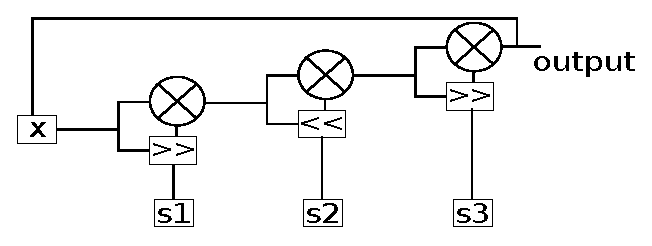
\includegraphics[width=6.5cm]{xorshift.eps}
  \label{xorshift verilog}}
  \subfigure[BBS]{\includegraphics[width=6.5cm]{bbs.eps}
  \label{BBS verilog}}
  \subfigure[The proposed CIPRNG]{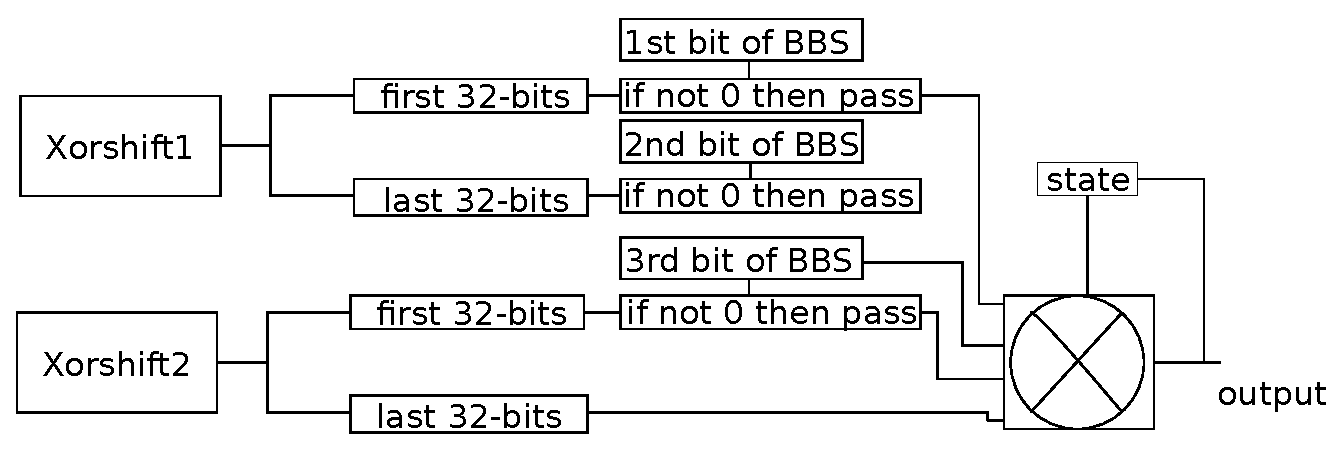
\includegraphics[width=10cm]{ci.eps}
  \label{CI verilog}}
\end{center}
\caption{The processing structure for BBS in FPGA (per clock step)}
\end{figure}
%In our program, we define 
%each FPGA clock positive edge, the XORshift will work, since these are simple processing for FPGA, every 
%clock step can lead to one output.

\subsubsection{Design of BBS}
Fig.\ref{BBS verilog} gives the proposed design of the BBS generator in FPGAs.
There are two inputs of $32$ bits, namely 
$b$ and $m$. 
Register $b$ stores the state of the system
at each time (after the square computation). 
$m$ is also a register that saves the value of $M$, which must not change.
Another register $b\_extend$ 
is used to combine $b$ to a data having $64$ bits, with a view to avoid overflow. 
After the last computation,
the three LSBs from the output of $\%$ are
taken as output. 
Let us notice that a BBS is
 performed at each time unit.

\begin{figure}
\begin{center}
  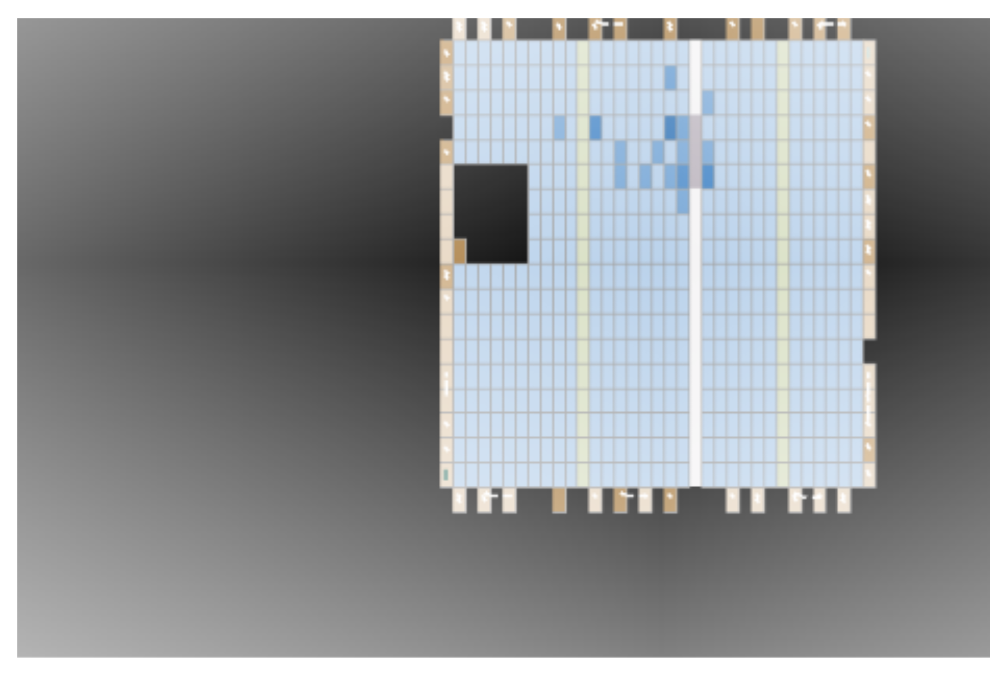
\includegraphics[width=6.5cm]{print.eps}
\end{center}
\caption{The sources cost in $EP2C8Q208C8$ FPGA board}
 \label{logic elements}
\end{figure}

\subsubsection{Design of the chaotic iterations}
Two XORshifts and one BBS are connected to work together, in order to compose the
proposed CIPRNG (see Fig.\ref{CI verilog}). 
As it can be shown, the three bits of the BBS output are switches for the corresponding $32$ bits XORshift outputs. Every round of the 
 processing costs two time units
 to be performed: in the first clock, 
the four PRNGs are processed in parallel,
whereas in the second one, the results of these generators are combined with 
the current state of the system, in order to produce the output of $32$ bits. The output sequence will be appended as Fig.~\ref{ci_OUTPUT} shown, started from the second clock (first clock BBS and XORshift use to initial the first output of CIPRNG).

\begin{figure}
\begin{center}
  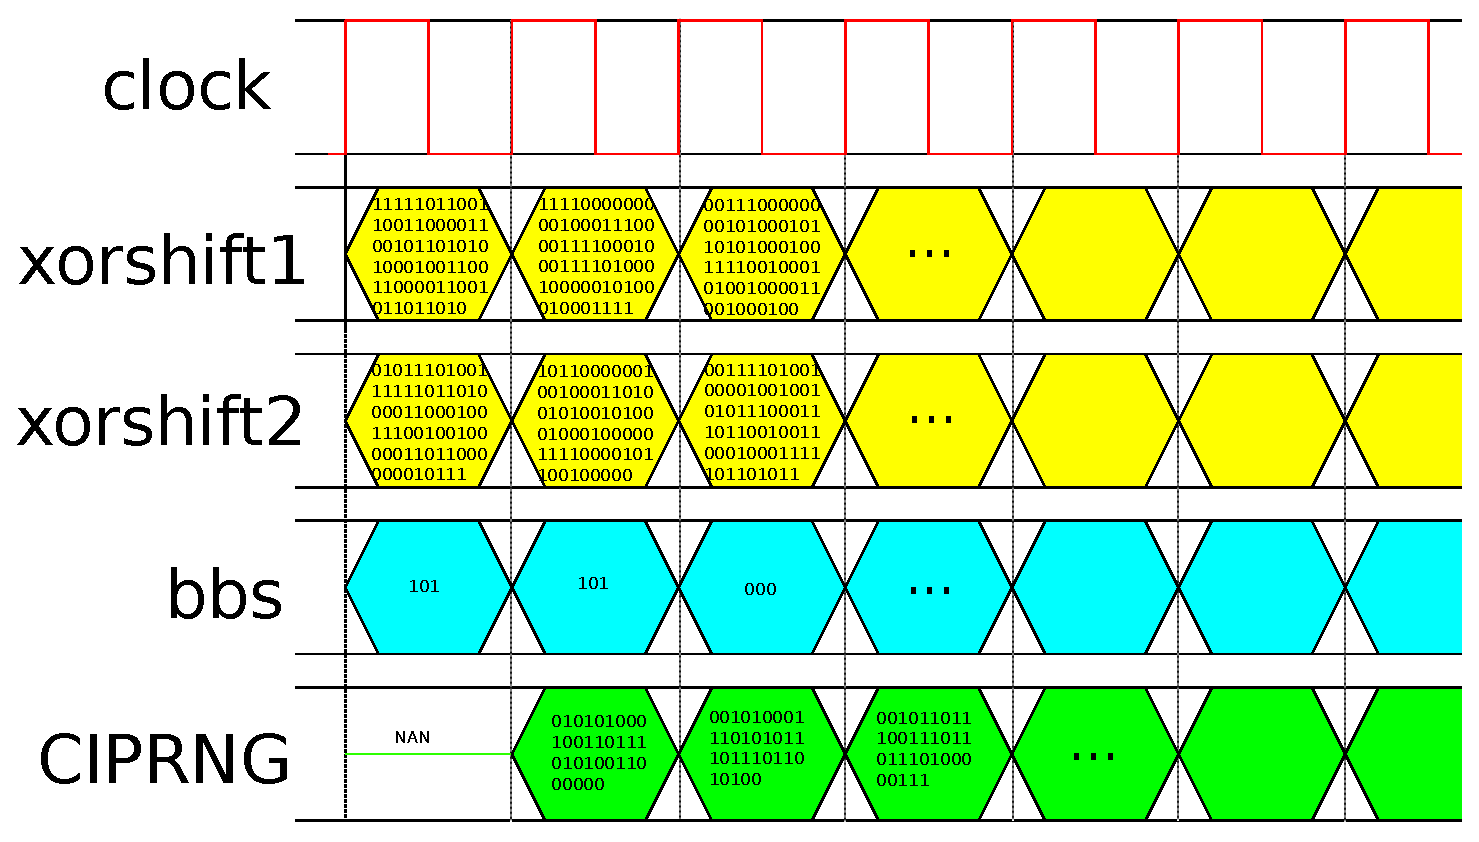
\includegraphics[width=14cm]{ci_OUTPUT.eps}
\end{center}
\caption{Working flow of each component for CIPRNG in FPGA}
 \label{ci_OUTPUT}
\end{figure}

In our experiments, the type $EP2C8Q208C8$ from Altera 
company's CYCLONE II FPGA series 
has been used. By default, its working
frequency is equal to $50$ MHz.
However, it is possible to increase it until
$200$ MHz by using the phase-lock loop (PLL) device.
In that situation, the CIPRNG designed on this
FPGA can produce about $6400$ Mbits per second
(that is, $200 (MHz) \times 32 (bits)$),
while using $3358$ of the $8256$ logic 
elements in $EP2C8Q208C8$ (see
Fig.\ref{logic elements}). 

In Chapter~\ref{Application Example}, an application of this 
CSPRNG designed on FPGA in the information 
hiding security fields is detailed, to show
that this hardware pseudorandom generator 
is ready to use.

\chapter{Randomness Quality of CIPRNGs}
\label{Statistical Tests for Randomness}
\minitoc

In this chapter, for having comparison criteria, some classical PRNGs are evaluated by the statistical tests introduced in Section~\ref{Some famous statistical tests of random number generators}, namely the NIST, DieHARD, Comparative tests, and TestU01 test suites.
Regarding these results, we will be able to easily verify the improvements of mixing
such generators using chaotic iterations. Statistical performances of the CIPRNG
versions 3 and 4 are then given in a second part of this chapter. 
Finally four versions of CIPRNGs are assembled together, and a 
comprehensive comparison among them is produced using the aforementioned tests 
(for the sake of fairness, all the CIPRNGs have received two XORshifts as
inputted generators). 
These results have been formerly published in~\cite{bfg12a:ip, bfgw11:ij, bfgw11:ip}.

\section{Test results for some PRNGs}
We present in this section the scores obtained by four well known PRNGs
against the usual batteries of tests. These generators are respectively
the BBS, Logistic, XORshift, and ISAAC ones (details for these
generators have been given in Section~\ref{The generation of pseudorandom sequence}).

%\subsection{NIST results}
\label{for nist}

Table~\ref{The passing1} contains the $\mathbb{P}_T$ values 
corresponding to the test results of sequences from BBS, Logistic map, XORshift, and ISAAC 
respectively. 
We can see that, except for ISAAC, all the proposed generators failed
in passing the NIST battery ($\mathbb{P}_T$ values should be $\in \llbracket 0, 1 \rrbracket$). Results are particularly bad for the BBS
generator, although this PRNG is known to be cryptographically secure.
It is not contradictory, as these bad scores are due to the small prime 
numbers that have been used here as parameters of this PRNG.


\begin{table}
\renewcommand{\arraystretch}{1.3}
\caption{NIST SP 800-22 test results ($\mathbb{P}_T$)}
\label{The passing1}
\centering
\begin{tabular}{lcccc}
\toprule
Test name & BBS &Logistic& XORshift& ISAAC\\ 

Frequency (Monobit) Test 			&0.32435	&0.53414		&0.14532		&0.67868 \\ 
Frequency Test within a Block			&0.00000	&0.00275		&0.45593		&0.10252 \\ 
Runs Test 					&0.00000	&0.00000		&0.21330		&0.69931\\ 
Longest Run of Ones in a Block Test 		&0.00000	&0.08051		&0.28966		&0.43727 \\
Binary Matrix Rank Test 			&0.00000	&0.67868		&0.00000		&0.89776\\ 
Discrete Fourier Transform (Spectral) Test	&0.00000	&0.57490		&0.00535		&0.51412 \\ 
Non-overlapping Template Matching Test* 	&0.00000	&0.28468		&0.50365		&0.55515\\ 
Overlapping Template Matching Test 		&0.00000	&0.10879		&0.86769		&0.63711\\ 
Universal Statistical Test 			&0.00000	&0.02054		&0.27570		&0.69931 \\ 
Linear Complexity Test		        	&0.04335	&0.79813		&0.92407		&0.03756\\ 
Serial Test* (m=10) 				&0.00000	&0.41542		&0.75792		&0.32681 \\ 
Approximate Entropy Test (m=10) 		&0.00000	&0.02054		&0.41902		&0.30412\\ 
Cumulative Sums (Cusum) Test* 			&0.00000	&0.60617		&0.81154		&0.36786\\ 
Random Excursions Test* 			&0.00000	&0.53342		&0.41923		&0.50711 \\ 
Random Excursions Variant Test* 		&0.00000	&0.28507		&0.52833		&0.40930\\ \hline
Success 					&2/15 	&14/15		&14/15			&15/15 \\ 
\bottomrule
\end{tabular}
\end{table}

%\subsection{DieHARD results}
\label{Subsec:DieHARD}

Table~\ref{Results of DieHARD battery} contains, for its part, 
the results derived from applying the DieHARD battery of 
tests to the four generators considered in this section.
Another time, ISAAC is the sole generator able to pass the
whole battery, whereas the logistic map and the XORshift
generators present correct results. BBS, for its part, shows
another time a very bad statistical profile.

\begin{tiny}
\begin{table}[!t]
\renewcommand{\arraystretch}{1.3}
\caption{Results of DieHARD battery of tests}
\label{Results of DieHARD battery}
\centering
\begin{tabular}{llcccc} \toprule
No. &Test name &BBS &Logistic& XORshift& ISAAC\\
1 & Overlapping Sum &Pass&Pass &Pass&Pass\\
2 & Runs Up 1 &Pass & Pass &Pass&Pass\\
&Runs Down 1 &Pass &Pass &Pass&Pass\\
&Runs Up 2 &Pass &Pass &Pass&Pass\\
&Runs Down 2 &Pass & Pass &Pass&Pass\\
3 & 3D Spheres &Fail &Pass &Pass&Pass\\
4 & Parking Lot &Fail &Pass &Pass&Pass\\
5 & Birthday Spacing &Fail &Pass &Pass&Pass\\
6 & Count the ones 1 &Fail &Pass &Fail&Pass\\
7 &Binary Rank $6 \times 8$ &Fail & Pass &Pass&Pass\\
8 &Binary Rank $31 \times 31$ &Fail &Pass &Fail&Pass\\
9 &Binary Rank $32 \times 32$ &Fail &Fail &Fail&Pass\\
10 &Count the ones 2 &Fail &Pass&Pass&Pass \\
11 &Bit Stream &Fail &Pass&Pass&Pass \\
12 &Craps Wins &Fail &Pass&Pass&Pass \\
&Throws &Fail &Pass&Pass&Pass\\
13 &Minimum Distance &Fail &Pass &Pass&Pass\\
14 &Overlapping Perm. &Fail&Pass &Pass&Pass\\
15 &Squeeze &Fail &Pass &Pass&Pass \\
16 &OPSO &Fail &Pass &Pass&Pass \\
17 &OQSO &Fail &Pass &Pass&Pass \\
18 &DNA &Fail &Fail &Pass &Pass\\
&Number of tests passed &2&16 &15&18 \\ \bottomrule
\end{tabular}
\end{table}
\end{tiny}

%\subsection{Comparative test parameters}



\begin{table}[!t]
\renewcommand{\arraystretch}{1.3}
\caption{Comparative test parameters with a $10^7$ bits sequence}
\label{Comparison3}
\centering
\begin{tabular}{lccccc}
 \toprule
Method			&Threshold values 	 &BBS		&Logistic	& XORshift	& ISAAC\\
Monobit			&3.8415			&0.3485&0.1280		&1.7053		&0.1401\\ \hline
Serial		&5.9915 		&2.0079	 &0.1302		&2.1466		&0.1430\\ \hline
Poker			&316.9194 		&387.7216 	&240.2893	&248.9318	&236.8670\\ \hline
Runs 			&55.0027		&33.2067	&26.5667	&18.0087	&34.1273 \\ \hline
Autocorrelation		&1.6449			&-0.7603	& 0.0373	&0.5099 	&-2.1712\\ 
\bottomrule
\end{tabular}
\end{table}

In Table~\ref{Comparison3} is given another comparison of the BBS,
Logistic map, XORshift, and ISAAC generators using the comparative test 
parameters previously introduced, BBS is the only one generator which can't pass.
Finally, Table~\ref{TestU011} gives the results derived from applying the 
TestU01 battery to these PRNGs.
\begin{table}[!t]
\renewcommand{\arraystretch}{1.3}
\caption{TestU01 Statistical Test}
\label{TestU011}
\centering
\begin{tabular}{lcccccc}
\toprule
Test name &Battery&Parameters &BBS& Logistic 		& XORshift	& ISAAC\\
Rabbit 				&$32\times10^9$ bits	&38 &26	&21	 	&14	&0	 \\
Alphabit 			&$32\times10^9$ bits	&17 &9	&16 		&9	&0	 \\
Pseudo DieHARD 			&Standard		&126 &8	&0 	 	&2	&0	\\
FIPS\_140\_2 			&Standard		&16&0	&0 		&0	&0	\\
Small Crush 			&Standard		&15 &10	&4 		&5	&0	 \\
Crush 				&Standard		&144 &117	&95 		&57	&0	 \\
Big Crush 			&Standard		&160 &134	&125 	 	&55	&0	 \\ \hline
Number of failures 		& 			&516 &304	&261 	 	&146	&0	 \\
\bottomrule
\end{tabular}
\end{table}



%\subsection{Conclusion}
From the results shown in the four tables, statistical quality of each generator 
considered in this section can be basically deduced. 
BBS used in our conditions is not able to
produce reasonable sequences, the bad scores of these tests mainly relates to its too small period value. 
For the logistic map, it sounds better than BBS. However, this generator only successfully pass the comparative parameters tests.
Furthermore, its speed is far from dominating the comparison. 
XORshift failed to succeed the Binary Matrix Rank Test (NIST). 
This test focuses on the rank of disjoint 
sub-matrices extracted from the entire sequence. 
Note that this 
test also appears in the DieHARD battery.  
Such results mean that the 
null hypothesis $H_0$ must be rejected for these two bit streams, where $H_0$ is: ``for each integer $t>0$, the vector $(u_0 , ..., u_{t-1})$ is uniformly 
distributed over the $t$-dimensional unit cube $[0, 1]^t$''.
Finally, ISAAC plays best in all.

\section{Test results and comparative analysis for the CIPRNG version 3}
%\subsection{Results of NIST}
\label{Results of NISTfor Version 3 CI}
 
The generator version 3 
of the CIPRNG family is based on a 
Lookup table (LUT).
We test it here with the parameter $N$
equal to $4$.
We can conclude from Table~\ref{The passing for Version 3 LUT CI} that, except for the mixture of BBS and XORshift, all 
possible couples have successfully passed the NIST statistical test suite. The statistic of inputed XORshift and Logistic map are improved, and there is no reduction for ISAAC.
Remark that the use of BBS, having poor statistical performances, leads to outputs of LUT-1 not very uniformly distributed. 

\begin{table}
\renewcommand{\arraystretch}{1.3}
\caption{NIST SP 800-22 test results ($\mathbb{P}_T$) for Version 3 LUT CI algorithms}
\label{The passing for Version 3 LUT CI}
\centering
\begin{tabular}{lccc}
\toprule
\multirow{4}*{Test name} & \multicolumn{3}{c}{Version 3 LUT CI}\\
& XORshift& ISAAC &BBS\\ 
& +& + & + \\ 
& XORshift& XORshift&XORshift\\\cmidrule(r){2-4}
Frequency (Monobit) Test 			&0.32435 		&0.33171		&0.00000 \\ 
Frequency Test within a Block			&0.85643		&0.42327		&0.13233\\ 
Runs Test 					&0.11623		&0.31908		&0.00000\\ 
Longest Run of Ones in a Block Test 		&0.74254		&0.86688		&0.00000 \\
Binary Matrix Rank Test 			&0.23224		&0.88317		&0.90311\\ 
Discrete Fourier Transform (Spectral) Test	&0.12316		&0.34578		&0.59559 \\ 
Non-overlapping Template Matching Test* 	&0.43295		&0.32637		&0.00000 \\ 
Overlapping Template Matching Test 		&0.31472		&0.55915		&0.00000\\ 
Universal Statistical Test 			&0.37864		&0.24925		&0.06282 \\ 
Linear Complexity Test			&0.65723		&0.31793		&0.94630 \\ 
Serial Test* (m=10) 				&0.43532		&0.55190		&0.00000 \\ 
Approximate Entropy Test (m=10) 		&0.34254		&0.12482		&0.00000\\ 
Cumulative Sums (Cusum) Test* 			&0.11272		&0.04065		&0.14139 \\ 
Random Excursions Test* 			&0.02003		&0.32275		&0.34625 \\ 
Random Excursions Variant Test* 		&0.43554		&0.234294		&0.55048\\ \hline
Success 					& 15/15			&15/15		&8/15	 \\ 
\bottomrule
\end{tabular}
\end{table}

%\subsection{Results of Diehard}
Table~\ref{Results of DieHARD battery of tests for Version 3 LUT CI algorithms} gives 
the results derived from applying the DieHARD battery of tests to the PRNGs considered in this chapter. 
For the same reasons as in the NIST test suite's results, the CIPRNG constituted by the mixture of 
BBS and XORshift is not able to pass all the DieHARD battery.

\begin{tiny}
\begin{table}
\renewcommand{\arraystretch}{1.3}
\caption{Results of DieHARD battery of tests for Version 3 LUT CI algorithms ($\mathsf{N}=4$)}
\label{Results of DieHARD battery of tests for Version 3 LUT CI algorithms}
\centering
\begin{tabular}{llcccc} \toprule
\multirow{3}*{No.} &\multirow{3}*{Test name} & \multicolumn{4}{c}{Version 3 CI}\\
&&Logistic& XORshift& ISAAC&BBS \\ 
&&+& +& + & + \\ 
&&Logistic& XORshift& XORshift&XORshift \\ \cmidrule(r){3-6}
1 & Overlapping Sum &Pass &Pass &Pass&Fail\\
2 & Runs Up 1 &Pass & Pass &Pass&Pass\\
&Runs Down 1 &Pass &Pass &Pass&Pass\\
&Runs Up 2 & Pass &Pass &Pass&Pass\\
&Runs Down 2 &Pass & Pass &Pass&Pass\\
3 & 3D Spheres &Pass &Pass &Pass&Fail\\
4 & Parking Lot &Pass &Pass &Pass&Pass\\
5 & Birthday Spacing &Pass &Pass &Pass&Fail\\
6 & Count the ones 1 &Pass &Pass &Pass&Fail\\
7 &Binary Rank $6 \times 8$ &Pass & Pass &Pass&Pass\\
8 &Binary Rank $31 \times 31$ &Pass &Pass &Pass&Fail\\
9 &Binary Rank $32 \times 32$ &Pass &Pass &Pass&Fail\\
10 &Count the ones 2 &Pass &Pass&Pass&Fail \\
11 &Bit Stream &Pass &Pass&Pass&Pass \\
12 &Craps Wins &Pass &Pass&Pass&Fail \\
&Throws &Pass &Pass &Pass&Pass\\
13 &Minimum Distance &Pass &Pass &Pass&Pass\\
14 &Overlapping Perm. &Pass &Pass &Pass&Pass\\
15 &Squeeze &Pass &Pass&Pass&Pass \\
16 &OPSO &Pass &Pass&Pass&Fail \\
17 &OQSO &Pass &Pass&Pass&Fail \\
18 &DNA &Pass &Pass&Pass &Fail\\
&Number of tests passed &18 &18 &18&8\\\bottomrule
\end{tabular}
\end{table}
\end{tiny}

%\subsection{Results of comparative test parameters}



\begin{table}
\renewcommand{\arraystretch}{1.3}
\caption{Comparative test parameters for Version 3 CI(X,Y) with a $10^7$ bits sequence ($\mathsf{N}=4$)}
\label{Comparison2 for Version 3 CI algorithms}
\centering
\begin{tabular}{lcccc}
\toprule
\multirow{4}*{Method} &\multirow{4}*{Threshold values} 	& \multicolumn{3}{c}{Version 3 CI}\\
&& XORshift& ISAAC&BBS\\ 
&& +& + & + \\ 
&& XORshift& XORshift&XORshift \\ \cmidrule(r){2-5}
Monobit			&3.8415				&3.5689		&0.9036		&1.5788 \\ \hline
Serial		&5.9915				&3.5765		&1.1229		&3.378\\ \hline
Poker			&316.9194			&123.6831	&173.8604		&209.3320\\ \hline
Runs 			&55.0027			&28.4237	&40.4606	&38.4153 \\ \hline
Autocorrelation		&1.6449				&0.3403		&0.1245		&-2.0276 \\ \bottomrule
\end{tabular}
\end{table}

We show in Table~\ref{Comparison2 for Version 3 CI algorithms} 
a ``comparative test parameters'' comparison between the three following CIPRNGs (version 3): CI(XORshift, XORshift),  
CI(ISAAC, XORshift), and CI(BBS, XORshift). 
The tests in this table consider sequences
having $10^7$ bits long.
The couple (BBS, XORshift) has finally 
beaten down all the corresponding batteries and pass the test. 
%\subsection{Results of TestU01}
Table~\ref{TestU01 for Version 3 CI}, for its
part, contains 
the results derived from applying the TestU01 battery to the PRNGs considered in this challenge.
\begin{table}
\renewcommand{\arraystretch}{1.3}
\caption{TestU01 Statistical Test for Version 3 CI algorithms ($\mathsf{N}=4$)}
\label{TestU01 for Version 3 CI}
\centering
\begin{tabular}{lccccc}
\toprule
\multirow{4}*{Test name} &&& \multicolumn{3}{c}{Version 3 CI}\\
&&&Logistic& ISAAC&BBS\\ 
&&&+& +& + \\ 
&&&Logistic& XORshift&XORshift\\ \cmidrule(r){4-6}
Rabbit 				&$32\times10^9$ bits	&38	&0 	&0 	& 18		 \\
Alphabit 			&$32\times10^9$ bits	&17 	&0 	&0 	& 	8	 \\
Pseudo DieHARD 			&Standard		&126 	&0 	&0 	& 11	\\
FIPS\_140\_2 			&Standard		&16 	&0 	&0 	& 0		\\
Small Crush 			&Standard		&15 	&0	&0	& 7		 \\
Crush 				&Standard		&144 	&0 	&0 	& 51		 \\
Big Crush 			&Standard		&160 	&0 	&0 	& 77		 \\ \hline
Number of failures 		& 			& 	&0 	&0	& 165		 \\
\bottomrule
\end{tabular}
\end{table}


%\subsection{Conclusion}

The results of the TestU01, NIST, Comparative test parameters, and DieHARD batteries of tests 
confirm that the CIPRNGs version 3 are all able to pass these tests. 
They are thus better than the version 1 while using less computational resources 
than the version number 2. However, in the situation using an classic cryptographically secure PRNG BBS, performances are completely deflated.
Finally, man can remark that performances are good when using ISAAC as 
inputted generator. However, ISAAC is very hard to implement in hardware, while
hardware implementation of CIPRNGs if one of the goal of this thesis.

From this tests study we can finally conclude that,
by using some well-defined Lookup Table and due to the rewrite of the way to generate strategies, 
the generator version 3 based on chaotic iterations works faster and has a better or equivalent (ISAAC) statistical profile than the
other generators previously tested in this chapter. Additionally, the speed of LUT CI is largely improved compared to 
the CIPRNGs version 1 and 2, and another time this version 3 may utilize any 
reasonable RNG as inputs (not necessarily XORshift, BBS, or ISAAC). 



\section{Tests results and comparative analysis for the CIPRNG version 4}
\label{test for Version 4 CI}
%\subsection{Results of NIST}
\label{Results of NIST for Version 4 CI}

We now investigate the case of the new
CIPRNG version 4, by starting first
to regard the NIST battery.
All the generators of this family tested
against this battery used a
$N = 32$ bits format. 
We can conclude from the results
summarized in Table~\ref{The passing for Version 4 CI} 
that all the PRNGs of this family have successfully passed the NIST statistical test suite. 
Indeed, even when using the deflated BBS, 
the CIPRNG version 4 using the couple (BBS, XORshift) still can provide a reasonable
statistical profile.

\begin{table}
\renewcommand{\arraystretch}{1.3}
\caption{NIST SP 800-22 test results ($\mathbb{P}_T$) for Version 4 CI algorithms}
\label{The passing for Version 4 CI}
\centering
\begin{tabular}{lccc}
\toprule
\multirow{4}*{Test name} & \multicolumn{3}{c}{Version 4 CI}\\
& XORshift& ISAAC &BBS\\ 
& +& + & + \\ 
& XORshift& XORshift&XORshift\\\cmidrule(r){2-4}
Frequency (Monobit) Test 			&0.21414 		&0.43622		&0.24563 \\ 
Frequency Test within a Block			&0.23423		&0.43536		&0.13233\\ 
Runs Test 					&0.56471		&0.23425		&0.23562 \\ 
Longest Run of Ones in a Block Test 		&0.33252		&0.86688		&0.12346 \\
Binary Matrix Rank Test 			&0.01450		&0.25689		&0.90311\\ 
Discrete Fourier Transform (Spectral) Test	&0.25462		&0.32324		&0.59559 \\ 
Non-overlapping Template Matching Test* 	&0.79521		&0.32637		&0.03984 \\ 
Overlapping Template Matching Test 		&0.69342		&0.55915		&0.13839\\ 
Universal Statistical Test 			&0.44654		&0.24925		&0.06282 \\ 
Linear Complexity Test			&0.97319		&0.31793		&0.54630 \\ 
Serial Test* (m=10) 				&0.58993		&0.55190		&0.98234 \\ 
Approximate Entropy Test (m=10) 		&0.39284		&0.12482		&0.12345\\ 
Cumulative Sums (Cusum) Test* 			&0.43582		&0.04065		&0.14139 \\ 
Random Excursions Test* 			&0.92001		&0.32275		&0.34625 \\ 
Random Excursions Variant Test* 		&0.24567		&0.234294		&0.55048\\ \hline
Success 					& 15/15			&15/15		&15/15	 \\ 
\bottomrule
\end{tabular}
\end{table}

%\subsection{Results of Diehard}
Table~\ref{Results of DieHARD battery of tests for Version 4 CI algorithms} gives 
the results derived from applying the DieHARD battery of tests to the PRNGs considered in this chapter. 
Results are closed to the ones produced
by the NIST test suite.
In particular, we can see that the mixing of 
BBS and XORshift shows better performance than in the other CIPRNG versions, and that 
all generators are successfully pass these tests.
\begin{tiny}
\begin{table}
\renewcommand{\arraystretch}{1.3}
\caption{Results of DieHARD battery of tests for Version 4 CI algorithms }
\label{Results of DieHARD battery of tests for Version 4 CI algorithms}
\centering
\begin{tabular}{llcccc} \toprule
\multirow{3}*{No.} &\multirow{3}*{Test name} & \multicolumn{4}{c}{Version 4 CI}\\
&&Logistic& XORshift& ISAAC&BBS \\ 
&&+& +& + & + \\ 
&&XORshift& XORshift& XORshift&XORshift \\ \cmidrule(r){3-6}
1 & Overlapping Sum &Pass &Pass &Pass&Pass\\
2 & Runs Up 1 &Pass & Pass &Pass&Pass\\
&Runs Down 1 &Pass &Pass &Pass&Pass\\
&Runs Up 2 & Pass &Pass &Pass&Pass\\
&Runs Down 2 &Pass & Pass &Pass&Pass\\
3 & 3D Spheres &Pass &Pass &Pass&Pass\\
4 & Parking Lot &Pass &Pass &Pass&Pass\\
5 & Birthday Spacing &Pass &Pass &Pass&Pass\\
6 & Count the ones 1 &Pass &Pass &Pass&Pass\\
7 &Binary Rank $6 \times 8$ &Pass & Pass &Pass&Pass\\
8 &Binary Rank $31 \times 31$ &Pass &Pass &Pass&Pass\\
9 &Binary Rank $32 \times 32$ &Pass &Pass &Pass&Pass\\
10 &Count the ones 2 &Pass &Pass&Pass&Pass \\
11 &Bit Stream &Pass &Pass&Pass&Pass \\
12 &Craps Wins &Pass &Pass&Pass&Pass \\
&Throws &Pass &Pass &Pass&Pass\\
13 &Minimum Distance &Pass &Pass &Pass&Pass\\
14 &Overlapping Perm. &Pass &Pass &Pass&Pass\\
15 &Squeeze &Pass &Pass&Pass&Pass \\
16 &OPSO &Pass &Pass&Pass&Pass \\
17 &OQSO &Pass &Pass&Pass&Pass \\
18 &DNA &Pass &Pass&Pass &Pass\\
&Number of tests passed &18 &18 &18&18\\\bottomrule
\end{tabular}
\end{table}
\end{tiny}
%
%\subsection{Results of comparative test parameters}
%
%
%
\begin{table}
\renewcommand{\arraystretch}{1.3}
\caption{Comparative test parameters for Version 4 CI(X,Y) with a $10^7$ bits sequence}
\label{Comparison2 for Version 4 CI algorithms}
\centering
\begin{tabular}{lcccc}
\toprule
\multirow{4}*{Method} &\multirow{4}*{Threshold values} 	& \multicolumn{3}{c}{Version 3 CI}\\
&& XORshift& ISAAC&BBS\\ 
&& +& + & + \\ 
&& XORshift& XORshift&XORshift \\ \cmidrule(r){2-5}
Monobit			&3.8415				&1.0689		&0.9036		&0.5788 \\ \hline
Serial		        &5.9915				&0.5765		&1.0229		&1.378\\ \hline
Poker			&316.9194			&223.6831	&133.8604		&182.3320\\ \hline
Runs 			&55.0027			&28.4237	&13.4606	&12.4153 \\ \hline
Autocorrelation		&1.6449				&1.3403		&0.1845		&-0.7276 \\ \bottomrule
\end{tabular}
\end{table}
We then produce in Table~\ref{Comparison2 for Version 4 CI algorithms} 
a comparison between CI(XORshift, XORshift), 
CI(ISAAC, XORshift), and CI(BBS, XORshift), all
in version 4,
using a ``comparative test parameters'' approach. 
According to these $10^7$ bits long sequence tests, the considered generators all show very good statistical performances.
%\subsection{Results of TestU01}
Finally, Table~\ref{TestU01 for Version 4 CI} gives 
the results against TestU01. 
We can see no failure at all, which is very
remarkable.
\begin{table}
\renewcommand{\arraystretch}{1.3}
\caption{TestU01 Statistical Test for Version 4 CI algorithms ($\mathsf{N}=4$)}
\label{TestU01 for Version 4 CI}
\centering
\begin{tabular}{lccccc}
\toprule
\multirow{4}*{Test name} &&& \multicolumn{3}{c}{Version 4 CI}\\
&&&Logistic& ISAAC&BBS\\ 
&&&+& +& + \\ 
&&&XORshift& XORshift&XORshift\\ \cmidrule(r){4-6}
Rabbit 				&$32\times10^9$ bits	&0	&0 	&0 	& 0		 \\
Alphabit 			&$32\times10^9$ bits	&0 	&0 	&0 	& 	0	 \\
Pseudo DieHARD 			&Standard		&0 	&0 	&0 	& 0	\\
FIPS\_140\_2 			&Standard		&0 	&0 	&0 	& 0		\\
Small Crush 			&Standard		&0 	&0	&0	& 0		 \\
Crush 				&Standard		&0 	&0 	&0 	& 0		 \\
Big Crush 			&Standard		&0 	&0 	&0 	& 0		 \\ \hline
Number of failures 		& 			&0 	&0 	&0	& 0		 \\
\bottomrule
\end{tabular}
\end{table}


%\subsection{Conclusion}

\medskip

The results of the TestU01, NIST, Comparative test parameters, and DieHARD batteries of tests confirm that the proposed 
chaotic iteration based generators
are all able to pass these tests.

These results have been obtained on an INTEL i5 dual 
core computer, with 2.3 GHz CPUs and 4GB of RAM memory.
As only $7$ hours have been required to finish the
biggest test (namely, the BigCrush in TestU01), we can claim that
this new version of a secured CIPRNG is very efficient.
Indeed, we can conclude from these tests that 
the
CIPRNG version 4 family realizes a great compromise among security, statistical performances, and efficiency. 
It thus can be considered as very suitable 
both for software and hardware implementations.

%This Version 4 CI PRNG based on discrete chaotic iterations is able to utilize any reasonable RNG as inputs. For demonstration purposes, XORshift, BBS, ISAAC are adopted here. 


\section{Assessment of four versions of CIPRNGs schemes}

In this section, we investigate more deeply 
the statistical comparison between the four 
versions of CIPRNGs under statistical aspects. 
To do so, all the tested CIPRNGs are embedding 
only $32$-bit XORshifts as inputted generators, and the values of the parameter $N$ are the most optimized according to previous experiments,
that is, $N=4$ for versions 1 and 3, and 
$N=32$ for the other versions. To be attention that two inputed generators are used for CIPRNG Version 1-3, and four inputed generators for CIPRNG Version 4.

\subsection{NIST evaluation}

We can firstly remark from Table~\ref{The passing} that XORshift has failed 1 test, whereas all
the versions of CI(XORshift, XORshift) have successfully passed the NIST statistical test suite. %This result shows the good behavior of both PRNGs in the aforementioned basic tests that evaluate the independence of real numbers.

\begin{table}
\renewcommand{\arraystretch}{1.3}
\caption{NIST SP 800-22 test results ($\mathsf{N}=4$ for Version 1 and 3 CIPRNG,$\mathsf{N}=32$ for XORshift generator, Version 2 and 4 CIPRNG )}
\label{The passing}
\centering
\begin{tabular}{|l||c|c|c|c|c|}
\hline
PRNG & Classic & \multicolumn{4}{c|}{CI PRNG versions}\\ \hline\hline
Method &XORshift& 1 & 2 & 3 &  4\\ \hline

FT			&0.1453&0.5955&0.4744&0.3257 & 0.8841 \\ \hline
FBT			&0.4553&0.5524&0.8970 & 0.1231 &0.4197\\ \hline
RT					&0.2134&0.4551&0.8161&0.9826&0.0253 \\ \hline
LROBT 		&0.2890&0.0126&0.7398&0.4892&0.3346 \\ \hline
BMRT 			&0.0000&0.6126&0.2621&0.1005&0.4456\\ \hline
DFTT	&0.0051&0.0102&0.1071 &0.8331 &0.6433\\ \hline
NOTMT* 	&0.5036&0.5322&0.4499 & 0.3031 & 0.7001 \\ \hline
OTMT 		&0.8676&0.3345&0.5141& 0.0925 &0.7739\\ \hline
MUST			&0.2757&0.0329&0.6786&0.6642&0.5031\\ \hline
LCT		&0.9240&0.4011&0.6579&0.5173&0.8077\\ \hline
ST* (m=10) 				&0.7579&0.0133&0.4253&0.3301&0.9281\\ \hline
AET (m=10) 		&0.4190&0.1373&0.6371&0.7181&0.0345\\ \hline
CST* 			&0.8115&0.0464&0.2796&0.3872&0.4011\\ \hline
RET* 			&0.4192&0.5036&0.2874 &0.9381 &0.1963\\ \hline
REVT* 		&0.5283&0.3477&0.4866& 0.4026 &0.5120\\ \hline
Success 					& 14/15	& 15/15& 15/15&15/15 &15/15 \\ \hline

\end{tabular}
\end{table}

\subsection{Diehard}
\label{Subsec:DieHARD}

Table~\ref{Results of DieHARD battery of tests} gives the results derived from applying the DieHARD battery of tests to the PRNGs considered in this section. As it can be observed, the results of XORshift failing the individual tests ``Count the ones 1'', ``Binary Rank $31 \times 31$'', and ``Binary Rank $32 \times 32$'' show that, in the random numbers obtained with the XORshift generator alone, only the least significant bits seem to be independent. This explains the poor behavior of this PRNG in the aforementioned basic tests that evaluate the independence of real numbers. But the generator based on discrete chaotic iterations (CIPRNGs versions 1-4) can get this problem over and pass all the DieHARD battery of tests. 
This proves that the
statistics of the given generator have been improved thanks to chaotic iterations.

\begin{tiny}
\begin{table}[!t]
\renewcommand{\arraystretch}{1.3}
\caption{Results of DieHARD battery of tests }
\label{Results of DieHARD battery of tests}
\centering
\begin{tabular}{llccccc} \toprule
\textbf{No.} &\textbf{Test name} &Classic &\multicolumn{4}{c}{\textbf{CI PRNG versions}} \\ \cmidrule(r){3-7}
& & XORshift &1 & 2 & 3 & 4\\ \midrule
1 & Overlapping Sum &Pass &Pass &Pass&Pass &Pass\\
2 & Runs Up 1 &Pass & Pass &Pass&Pass &Pass\\
&Runs Down 1 &Pass &Pass &Pass&Pass &Pass\\
&Runs Up 2 & Pass &Pass &Pass&Pass &Pass\\
&Runs Down 2 &Pass & Pass &Pass&Pass &Pass\\
3 & 3D Spheres &Pass &Pass &Pass&Pass &Pass\\
4 & Parking Lot &Pass &Pass &Pass&Pass &Pass\\
5 & Birthday Spacing &Pass &Pass &Pass&Pass &Pass\\
6 & Count the ones 1 &Fail &Pass &Pass&Pass &Pass\\
7 &Binary Rank $6 \times 8$ &Pass & Pass &Pass&Pass &Pass\\
8 &Binary Rank $31 \times 31$ &Fail &Pass &Pass&Pass &Pass\\
9 &Binary Rank $32 \times 32$ &Fail &Pass &Pass&Pass &Pass\\
10 &Count the ones 2 &Pass &Pass&Pass&Pass &Pass \\
11 &Bit Stream &Pass &Pass&Pass &Pass &Pass\\
12 &Craps Wins &Pass &Pass&Pass &Pass &Pass \\
&Throws &Pass &Pass &Pass&Pass &Pass\\
13 &Minimum Distance &Pass &Pass &Pass&Pass &Pass\\
14 &Overlapping Perm. &Pass &Pass &Pass&Pass &Pass\\
15 &Squeeze &Pass &Pass&Pass &Pass &Pass\\
16 &OPSO &Pass &Pass&Pass &Pass &Pass\\
17 &OQSO &Pass &Pass&Pass &Pass &Pass\\
18 &DNA &Pass &Pass&Pass &Pass &Pass\\
&Number of tests passed &15 &18 &18&18&18\\\bottomrule
\end{tabular}
\end{table}
\end{tiny}

\subsection{Comparative test parameters}

\begin{table}
\renewcommand{\arraystretch}{1.3}
\caption{Comparison with CIPRNGs(XORshift,XORshift) for a $10^7$ bits sequence($\mathsf{N}=32$)}
\label{Comparison22}
\centering
\begin{tabular}{lcccccc}
\toprule
PRNGS & & Classic & \multicolumn{4}{c}{CI PRNG versions}\\
Method & The threshold values& XORshift & 1& 2 &3 & 4 \\ \hline 
 
Monobit			&3.84		&1.71		&2.77		&0.33	&0.02 &0.60 \\ \hline
Serial		&5.99		&2.15		&2.88		&0.74		&1.05 &0.04 \\ \hline
Poker	&316.91	&248.93	&222.36	&262.82		 &217.5 &209.9\\ \hline
Runs 			&55.00	&18.01	&21.92	&16.78	&22.77 &17.34 \\ \hline
Autocorrelation		&1.64		&0.50		&0.02		&0.08 &1.33 &0.81		 \\\hline
Time			&Second		&7.10s		&31.41s	&24.32s & 17.24s &9.12s \\		 
\bottomrule
\end{tabular}
\end{table}



We show in Table~\ref{Comparison22} a comparison between the CIPRNG(XORshift, XORshift) versions 1-4  and a simple XORshift. Time (in seconds) is related to the duration needed by each algorithm to generate a $10^8$ bits long sequence.
The tests have been conducted using the same computer and compiler with the same optimization settings for both algorithms (i5 dual cpu, 2300MHz, 4GB memory, gcc compiler, and UBUNTU system), in order to make the
comparisons as fair as possible. No doubt that CIPRNG Version shows very great efficiency, it is only slower than the fast generator XORshift.


\begin{figure}
\centering
% \psfig{figure=2.eps,height=5in,width=3.5in}
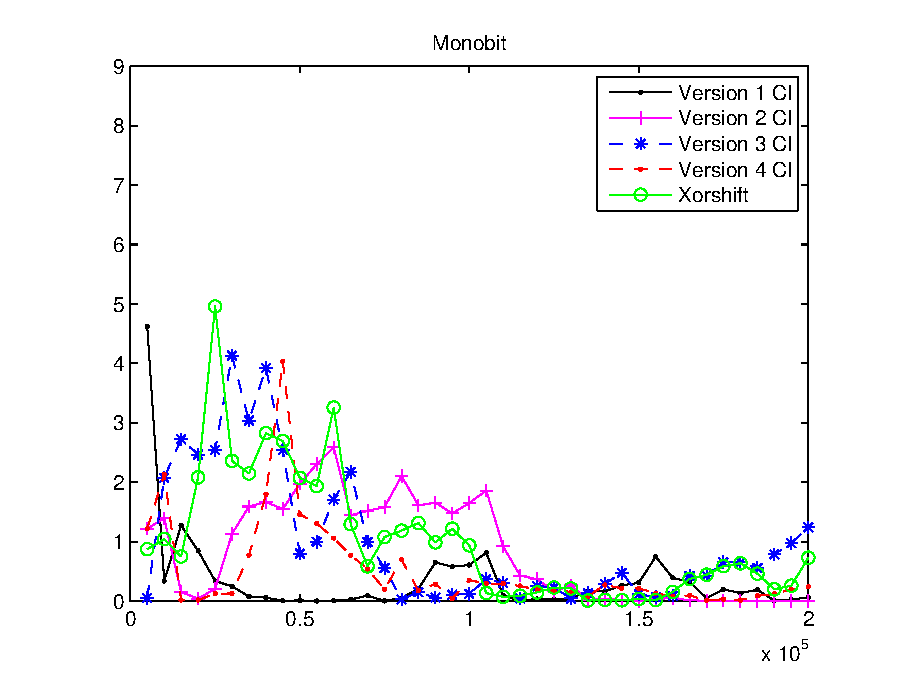
\includegraphics[scale=0.8]{monobits.eps}
% \includegraphics[width=3.7in]{4tests.eps}
\caption{Comparison of monobits tests}
\label{monobits}
\end{figure}

As a comparison of the overall stability of these PRNGs, similar tests have been computed for different sequence lengths (see Fig.\ref{monobits} - Fig.\ref{autocorrelation}).
For the monobit test comparison (Fig.\ref{monobits}), XORshift and CI(XORshift, XORshift) PRNGs versions 2-4 present the same values. They are stable in a low level that never exceeds 1.2. Indeed, the new generators distributes very randomly the zeros and ones, whatever the length of the desired sequence. 
It can also be remarked that the XORshift generator presents the worst performance, but the values are within the standard boundary.
\begin{figure}
\centering
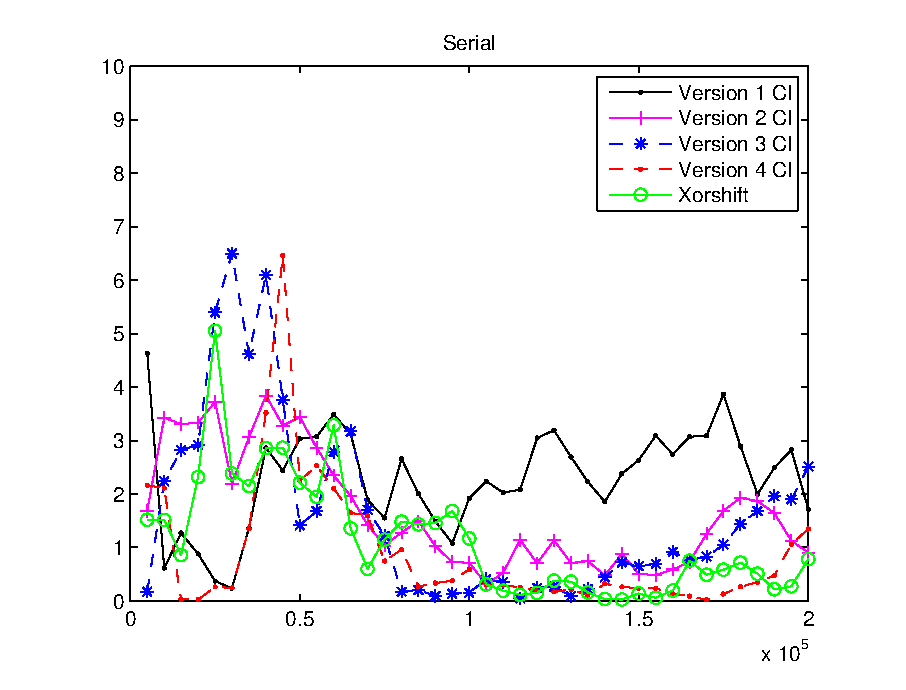
\includegraphics[scale=0.8]{serial.eps}
\caption{Comparison of serial tests}
\label{serial}
\end{figure}

Figure~\ref{serial} shows the serial test comparison. The CIPRNGs outputs outperform this test, for lengths between $2\times 10^4$ and $5 \times 10^4$. 
We can remark too that versions 2 and 3 express a little overflow, even if all generators occurrences of 00, 01, 10, and 11 are very closed to each other.

\begin{figure}
\centering
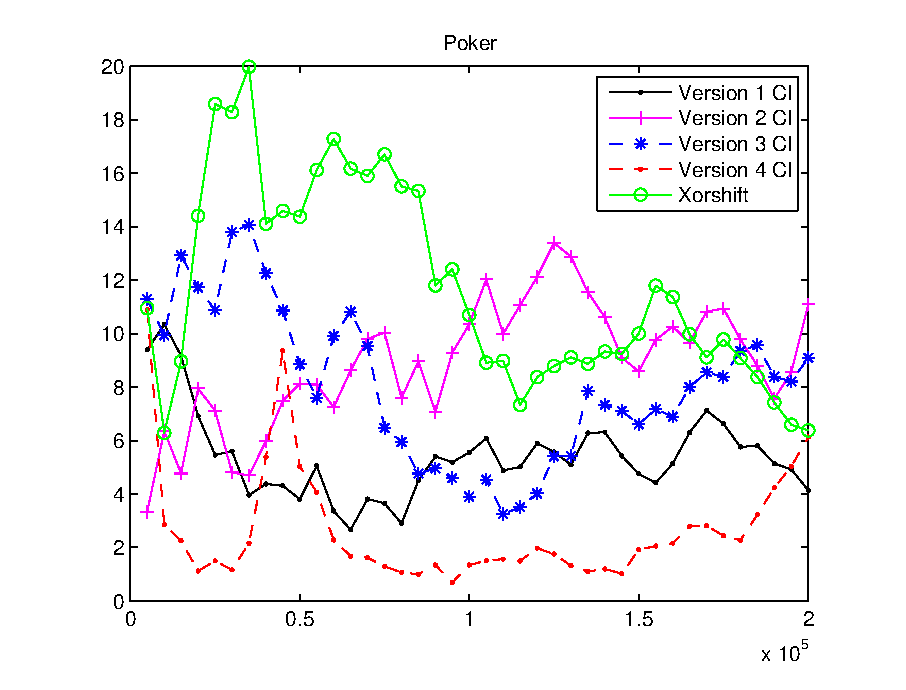
\includegraphics[scale=0.8]{poker.eps}
% \includegraphics[width=3.7in]{4tests.eps}
\caption{Comparison of poker tests}
\label{poker}
\end{figure}

The poker test comparison with $m=8$ is shown in Fig.~\ref{poker}. For some lengths, XORshift is not very stable, whereas 
all the CIPRNGs present good scores (values are lower than the given threshold). 
%The reasons explaining this bad result can be, among other:
Indeed, the value of $m$ and the length of the sequences should be enlarged to be certain that the chaotic iterations express totally their complex behavior. By doing so, the performances of our generators in the poker test can be improved.
%but here we only achieve $2 \times 10^5$ sequence length, then m must be smaller than 13 to comply with the rule, if the sequence length is more, the performance of CI might be better.

\begin{figure}
\centering
% \psfig{figure=2.eps,height=5in,width=3.5in}
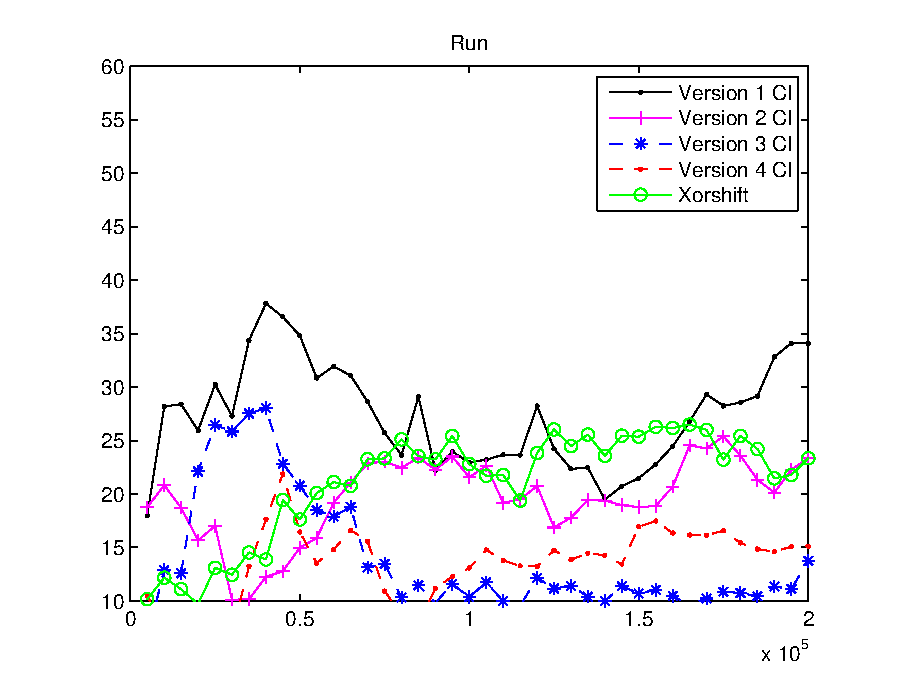
\includegraphics[scale=0.8]{runs.eps}
% \includegraphics[width=3.7in]{4tests.eps}
\caption{Comparison of runs tests}
\label{runs}
\end{figure}

The graphs of the CI generators are the most stable ones during the runs test comparison (Fig.\ref{runs}). Moreover, this trend is reinforced when the lengths of the tested sequences are increased.
%
%
\begin{figure}
\centering
% \psfig{figure=2.eps,height=5in,width=3.5in}
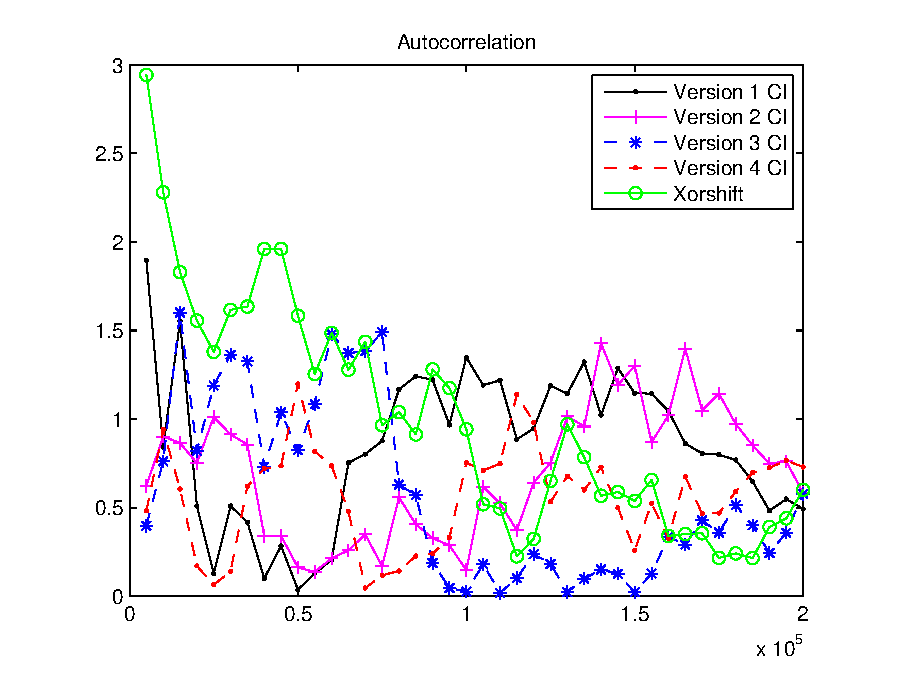
\includegraphics[scale=0.8]{autocorrelation1.eps}
% \includegraphics[width=3.7in]{4tests.eps}
\caption{Comparison of autocorrelation tests}
\label{autocorrelation}
\end{figure}
%
%
The comparison of autocorrelation tests is presented in Fig.~\ref{autocorrelation}. We can see that the CI generators clearly dominate these tests.

As a conclusion of all this study, we can finally claim that the CIPRNGs, whose newer versions run faster than theirs former ones, outperform all of the other generators in these statistical tests, especially when producing long output sequences.



%
%\subsection{A flexible output}
%
%We assume that the initial state $X$ is given as arrays of N-bit integers. Thus, the output size can be flexibly chosenell as $N$. Our PRNGs can generate discrete numbers
%where the number of states could not match to a power of 2, which is suitable for stochastic differential equations as an example.(An attractive property of discrete random numbers is that they
%require a small number of random bits--3 bits)~\cite{Ladd20092140}.
%Moreover, due to the fact that CI process is a simple bitwise change, the speed of output integers and binary numbers is almost the same. 
%
%In the following section, we will discuss the security level for various $N$ by Statistical test.
%For both CI generator, various $N$ can pass all the NIST and DIEHARD test. Table~\ref{TestU01 Statistical Test} gives the results derived from applying the TestU01 battery of tests to the PRNGs considered in this work. As observed,an conclude that the effective range of $N$ for Version 2 CI is bigger than for Version 1 CI by TestU01. And also, this new scheme for obtaining a PRNG by combining two XORshift generators in CI give better properties than the old one (and the individual XORshift alone). It can be observed that the XORshift generator fails 146 tests.
%
%\begin{table}[!t]
%\begin{small}
%\centering
%\renewcommand{\arraystretch}{1.3}
%\caption{TestU01 Statistical Test}
%\label{TestU01 Statistical Test}
%\centering
%\begin{tabular}{cccccccccc}\toprule
%\textbf{CI PRNG}&\textbf{Battery}&\textbf{N=2}&\textbf{N=4}&\textbf{N=8}&\textbf{N=16}&\textbf{N=32} \\\midrule
%
%\multirow{7}*{\textbf{Version 1 CI}}&Rabbit	 	&2	&2	&2	&2	&3 \\
%\multirow{7}*{\textbf{(XORshift,XORshift)}}&Alphabit 				&0	&0	&0	&2	&2 \\
%&Pseudo DieHARD 								&0	&0	&0	&0	&0 \\
%&FIPS\_140\_2 		 							&0	&0	&0	&0	&0 \\
%&Small Crush 		 							&0	&0	&0	&1	&0 \\
%&Crush 		 								&4	&4	&9	&16	&46 \\
%&Big Crush 									&5	&3	&18	&30	&78 \\ 
%\\
%&Number of failures 	 							&11	&9	&29	&51	&129 \\
%\bottomrule
%
%\multirow{7}*{\textbf{Version 2 CI}}&Rabbit 					0	&0	&0	&0	&0 \\
%\multirow{7}*{\textbf{(XORshift,XORshift)}}&Alphabit 				&4	&0	&0	&0	&0 \\
%&Pseudo DieHARD 	 							&8	&2	&0	&0	&0 \\
%&FIPS\_140\_2		 							&2	&0	&0	&0	&0 \\
%&Small Crush 		 							&0	&0	&0	&0	&0 \\
%&Crush 										&0	&0	&0	&0	&0 \\
%&Big Crush 		 							&0	&0	&0	&0	&0 \\ 
%\\
%&Number of failures 	 							&14	&2	&0	&0	&0 \\
%\bottomrule
%\end{tabular}
%\end{small}
%\end{table}
%
%

%\include{part2_CIPRNGFamily}
\chapter{An optimization technique on pseudorandom generators based on chaotic iterations}
\minitoc
\label{An optimization technique on pseudorandom generators based on chaotic iterations}

In this chapter, the behavior of our CIPRNGs regarding 
the statistics of the inputted generators are carried out systematically, and the results are discussed.
Here, CIPRNG Version 1, Version 2 and XOR CIPRNG method are applied to experimented.
Indeed PRNGs are often based on modular arithmetic, logical operations like bitwise exclusive or (XOR), and on circular shifts of
bit vectors.
However the security level of some PRNGs of this kind has been revealed inadequate by today's standards.
Since different biased generators can possibly have their own side effects when inputted into our mixed generators, it is normal to enlarge the set of tested inputted PRNGs, to determine if the observed improvement still remains.
We will thus show in this chapter that the intended statistical improvement is really effective for all of these most famous generators. To be notice, we have formally published the works in \cite{bfg12a:ip}.



\section{Presentation of new well known generators}
\label{The generation of pseudo-random sequence}

\subsection{Introduction}

Knowing that there is no universal generator, it is strongly recommended to test a stochastic application with a large set of different PRNGs~\cite{DavidRC2003643}. Such 
generators can be classified in four major classes: linear generators, lagged generators, inversive generators, and mix generators:
\begin{itemize}
 \item \textbf{Linear generators}, defined by a linear recurrence, are the most commonly analyzed and utilized generators. The main linear generators are LCGs and MLCG.
 \item \textbf{Lagged generators} have a general recursive formula that use various previously computed terms in the determination of the new sequence value.
 \item \textbf{Inversive congruential generators} form a recent class of generators that are based on the principle of congruential inversion.
 \item \textbf{Mixed generators} result from the need for sequences of better and better quality, or at least longer periods. This usually leads to mix different types of PRNGs, as follows: $x^i=y^i\oplus z^i$
\end{itemize}


For instance, inversive generators are very interesting for verifying simulation results obtained with a linear congruential generator (LCG),
because their internal structure and correlation behavior strongly differ from what LCGs produce.
Since these generators have revealed several issues, some scientists refrain from using them.
In what follows, chaotic properties will be added to these PRNGs, leading to noticeable improvements observed by statistical tests.
%Thus it helps scientists to enhance their habits by facilitating the use of sequences generated by generators that maybe they would not have used otherwise.
Let us firstly explain with more details the generators studied in this research work (for a synthetic view, see Fig.~\ref{Ontological class hierarchy of RNGs}).

\begin{figure}
\centering
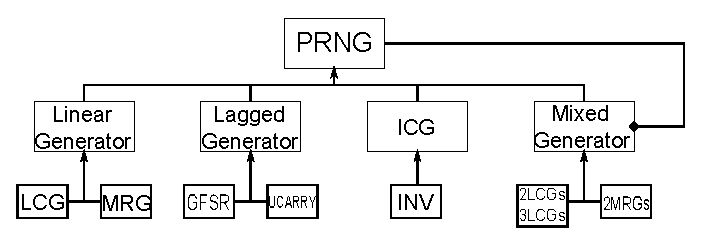
\includegraphics[width=3.5in]{TYPEPRNG.eps}
\DeclareGraphicsExtensions.
\caption{Ontological class hierarchy of PRNGs}
\label{Ontological class hierarchy of RNGs}
\end{figure}

\subsection{Details of some Existing Generators}

Here are the modules of PRNGs we have chosen to experiment.

\subsubsection{LCG}
This PRNG implements either the simple or the combined linear congruency generator (LCGs). The simple LCG is defined by the recurrence:
\begin{equation}
x^n = (ax^{n-1} + c)~mod~m
\label{LCG}
\end{equation}
where $a$, $c$, and $x^0$ must be non-negative and less than $m$~\cite{Lecuyer2009} integers. In what follows, 2LCGs and 3LCGs refer as two (resp. three) combinations of such LCGs.
For further details, see~\cite{combined_lcg}.

\subsubsection{MRG}
This module implements multiple recursive generators (MRGs), based on a linear recurrence of order integer $k$, modulo $m$~\cite{Lecuyer2009}:
\begin{equation}
x^n = (a^1x^{n-1}+~...~+a^kx^{n-k})~mod~m
\label{MRG}
\end{equation}
Combination of two MRGs (referred as 2MRGs) is also used in this chapter.

\subsubsection{UCARRY}
Generators based on linear recurrences with carry are implemented in this module. This includes the add-with-carry (AWC) generator, based on the recurrence:
\begin{equation}
\label{AWC}
\begin{array}{l}
x^n = (x^{n-r} + x^{n-s} + c^{n-1})~mod~m, \\
c^n= (x^{n-r} + x^{n-s} + c^{n-1}) / m, \end{array}\end{equation}
with output: $x^i/m$. The $k$ initial values $(x^0,... ,x^{k-1})$ is firstly set with random integers.
the $k = max\{r, s\}$ (the bigger one assigned to $k$), and $c$ contains $c^0$. Restrictions: $0 < s, 0 < r, r\neq s$ and $c = 0 or 1$.

The SWB generator, having the recurrence:
\begin{equation}
\label{SWB}
\begin{array}{l}
x^n = (x^{n-r} - x^{n-s} - c^{n-1})~mod~m, \\
c^n=\left\{
\begin{array}{l}
1 ~~~~~\text{if}~ (x^{i-r} - x^{i-s} - c^{i-1})<0\\
0 ~~~~~\text{else},\end{array} \right. \end{array}\end{equation}
with output is $x^i/m$. The vector $S[0..(k-1)]$ contains
the $k$ initial values $(x^0,... x^{k-1})$, where $k = max\{r, s\}$, and $c$ contains $c0$. Restrictions : $0 < s,0 < r, r 6= s$ and $c = 0$ or $1$.
And the SWC generator designed by R. Couture, which is based on the following recurrence:
\begin{equation}
\label{SWC}
\begin{array}{l}
x^n = (a^1x^{n-1} \oplus ~...~ \oplus a^rx^{n-r} \oplus c^{n-1}) ~ mod ~ 2^w, \\
c^n = (a^1x^{n-1} \oplus ~...~ \oplus a^rx^{n-r} \oplus c^{n-1}) ~ / ~ 2^w. \end{array}\end{equation}
with output is $x^i/2^w$. The vector $(x^n,...x^{n-r+1}, c^n)$ is the state of the generator. The array $A[0..h-1]$ contains the polynomials $a^1,...,a^r$. Each even element stands for a polynomial number and the next
element stands for the corresponding nonzero coefficient number of that polynomial. The vector
$S[0..r-1]$ gives the initial values of $(x^0,...,x^{r-1})$ and $c$ is the initial carry. Restrictions: $0 < r,$
and $w \leq 32$.

\subsubsection{GFSR}
This module implements the generalized feedback shift register (GFSR) generator, that is:
\begin{equation}
x^n = x^{n-r} \oplus x^{n-k}
\label{GFSR}
\end{equation}
Where the $x$ sequence are initial with some random positive integers, $n>k$ and $n>r$.

\subsubsection{INV}
Finally, this module implements the nonlinear inversive generator, as defined in~\cite{Lecuyer2009}, which is:

\begin{equation}
\label{INV}
\begin{array}{l}
x^n=\left\{
\begin{array}{ll}
(a^1 + a^2 / z^{n-1})~mod~m & \text{if}~ z^{n-1} \neq 0 \\
a^1 & \text{if}~  z^{n-1} = 0 .\end{array} \right. \end{array}\end{equation}

The generator computes $z$ via the modified Euclid algorithm (see \cite{Lecuyer2009}). If $m$ is prime and if $p(x) = x^2 -a^1 x -a^2$ is a primitive polynomial modulo $m$, then the generator has maximal period $m$. Restrictions: $0 \leq z^0 < m, 0 < a^1 < m$ and $0 < a^2 < m$. Furthermore, $m$ must be a prime number, preferably large.

%\section{statistical tests}
%\label{Security analysis}
%
%%A theoretical proof for the randomness of a generator is impossible to give, therefore statistical inference based on observed sample sequences produced by the generator seems to be the best option.
%Considering the properties of binary random sequences, various statistical tests can be designed to evaluate the assertion that the sequence is generated by a perfectly random source. We have performed some statistical tests for the CIPRNGs proposed here. These tests include NIST suite~\cite{ANDREW2008} and DieHARD battery of tests~\cite{Marsaglia1996}. For completeness and for reference, we give in the following subsection a brief description of each of the aforementioned tests.
%
%\subsection{NIST statistical tests suite}
%
%Among the numerous standard tests for pseudo-randomness, a convincing way to show the randomness of the produced sequences is to confront them to the NIST (National Institute of  Standards and Technology) statistical tests, being an up-to-date tests suite proposed by the Information Technology Laboratory (ITL). A new version of the Statistical tests suite has been released in August 11, 2010.
%
%The NIST tests suite SP 800-22 is a statistical package consisting of 15 tests. They were developed to test the randomness of binary sequences produced by hardware or software based cryptographic pseudorandom number generators. These tests focus on a variety of different types of non-randomness that could exist in a sequence.
%
%For each statistical test, a set of $P-values$ (corresponding to the set of sequences) is produced.
%The interpretation of empirical results can be conducted in various ways.
%In this paper, the examination of the distribution of P-values to check for uniformity ($ P-value_{T}$) is used.
%The distribution of $P-values$ is examined to ensure uniformity.
%If $P-value_{T} \geqslant 0.0001$, then the sequences can be considered to be uniformly distributed.
%
%In our experiments, 100 sequences (s = 100), each with 1,000,000-bit long, are generated and tested. If the $P-value_{T}$ of any test is smaller than 0.0001, the sequences are considered to be not good enough and the generating algorithm is not suitable for usage.
%
%
%
%
%
%\subsection{DieHARD battery of tests}
%The DieHARD battery of tests has been the most sophisticated standard for over a decade. Because of the stringent requirements in the DieHARD tests suite, a generator passing this battery of
%tests can be considered good as a rule of thumb.
%
%The DieHARD battery of tests consists of 18 different independent statistical tests. This collection
% of tests is based on assessing the randomness of bits comprising 32-bit integers obtained from
%a random number generator. Each test requires $2^{23}$ 32-bit integers in order to run the full set
%of tests. Most of the tests in DieHARD return a $P-value$, which should be uniform on $[0,1)$ if the input file
%contains truly independent random bits.  These $P-values$ are obtained by
%$P=F(X)$, where $F$ is the assumed distribution of the sample random variable $X$ (often normal).
%But that assumed $F$ is just an asymptotic approximation, for which the fit will be worst
%in the tails. Thus occasional $P-values$ near 0 or 1, such as 0.0012 or 0.9983, can occur.
%An individual test is considered to be failed if the $P-value$ approaches 1 closely, for example $P>0.9999$.

\section{Results and discussion}
\label{Results and discussion}


\begin{sidewaystable}
\caption{NIST and DieHARD tests suite passing rates for PRNGs without CI}
\label{NIST and DieHARD tests suite passing rate the for PRNGs without CI}
\centering
\begin{tabular}{|l||c|c|c|c|c|c|c|c|c|c|}
    \hline\hline
Types of PRNGs & \multicolumn{2}{c|}{Linear PRNGs} & \multicolumn{4}{c|}{Lagged PRNGs} & \multicolumn{1}{c|}{ICG PRNGs} & \multicolumn{3}{c|}{Mixed PRNGs}\\ \hline
\backslashbox{\textbf{$Tests$}} {\textbf{$PRNG$}} & LCG& MRG& AWC & SWB  & SWC & GFSR & INV & LCG2& LCG3& MRG2 \\ \hline
NIST & 11/15 & 14/15 &\textbf{15/15} & \textbf{15/15}   & 14/15 & 14/15  & 14/15 & 14/15& 14/15& 14/15 \\ \hline
DieHARD & 16/18 & 16/18 & 15/18 & 16/18 & \textbf{18/18} & 16/18 & 16/18 & 16/18& 16/18& 16/18\\ \hline
\end{tabular}
\end{sidewaystable}



Table~\ref{NIST and DieHARD tests suite passing rate the for PRNGs without CI} shows the results on the batteries recalled in a
previous chapter, indicating that almost all the PRNGs introduced here cannot pass all their embedding tests. In other words, the statistical quality of these PRNGs cannot fulfill the up-to-date standards presented previously. We will show that the CIPRNG can solve this issue.

To illustrate the effects of this CIPRNG in detail, experiments will be divided in three parts:
\begin{enumerate}
  \item \textbf{Single CIPRNG}: The PRNGs involved into the chaotic iterations computing are of the same category.
  \item \textbf{Mixed CIPRNG}: Two different types of generators are mixed during the CIPRNG process.
  \item \textbf{Multiple CIPRNG}: The generator is obtained by repeating the composition of the iteration function as follows: $x^0\in \mathds{B}^{\mathsf{N}}$, and $\forall n\in \mathds{N}^{\ast },\forall i\in \llbracket1;\mathsf{N}\rrbracket,$
\begin{equation}
\begin{array}{l}
x_i^n=\left\{
\begin{array}{l}
x_i^{n-1}~~~~~\text{if}~S^n\neq i \\
\forall j\in \llbracket1;\mathsf{m}\rrbracket,f^m(x^{n-1})_{S^{nm+j}}~\text{if}~S^{nm+j}=i.\end{array} \right. \end{array}
\end{equation}
$m$ is called the \emph{functional power}.
\end{enumerate}


We have performed statistical analysis of each of the aforementioned CIPRNGs.
The results are reproduced in Tab.~\ref{NIST and DieHARD tests suite passing rate the for PRNGs without CI} and \ref{NIST and DieHARD tests suite passing rate the for single CIPRNGs}.
The scores written in boldface indicate that all the tests have been passed successfully, whereas an asterisk ``*'' means that the considered passing rate has been improved.
\subsection{Tests based on the Single CIPRNG}

\begin{sidewaystable}
\renewcommand{\arraystretch}{1.3}
\caption{NIST and DieHARD tests suite passing rates for PRNGs with CI}
\label{NIST and DieHARD tests suite passing rate the for single CIPRNGs}
\centering
  \begin{tabular}{|l||c|c|c|c|c|c|c|c|c|c|c|c|}
    \hline
Types of PRNGs & \multicolumn{2}{c|}{Linear PRNGs} & \multicolumn{4}{c|}{Lagged PRNGs} & \multicolumn{1}{c|}{ICG PRNGs} & \multicolumn{3}{c|}{Mixed PRNGs}\\ \hline
\backslashbox{\textbf{$Tests$}} {\textbf{$Single~CIPRNG$}} & LCG  & MRG & AWC & SWB & SWC & GFSR & INV& LCG2 & LCG3& MRG2 \\ \hline\hline
Version 1 CIPRNG\\ \hline \hline
NIST & \textbf{15/15} *  & \textbf{15/15} * & \textbf{15/15}   & \textbf{15/15}   & \textbf{15/15} * & \textbf{15/15} * & \textbf{15/15} *& \textbf{15/15} * & \textbf{15/15} * & \textbf{15/15} \\ \hline
DieHARD & \textbf{18/18} *  & \textbf{18/18} * & \textbf{18/18} *  & \textbf{18/18} *  & \textbf{18/18}  & \textbf{18/18} * & \textbf{18/18} *& \textbf{18/18} * & \textbf{18/18} *& \textbf{18/18} * \\ \hline
Version 2 CIPRNG\\ \hline \hline
NIST & \textbf{15/15} *  & \textbf{15/15} * & \textbf{15/15}   & \textbf{15/15}  & \textbf{15/15} * & \textbf{15/15} * & \textbf{15/15} *& \textbf{15/15} * & \textbf{15/15} * & \textbf{15/15} \\ \hline
DieHARD & \textbf{18/18} *  & \textbf{18/18} * & \textbf{18/18} * & \textbf{18/18} * & \textbf{18/18}  & \textbf{18/18} * & \textbf{18/18} * & \textbf{18/18} * & \textbf{18/18} *& \textbf{18/18} *\\ \hline
Xor CIPRNG\\ \hline\hline
NIST & 14/15*& \textbf{15/15} *   & \textbf{15/15}   & \textbf{15/15}   & 14/15 & \textbf{15/15} * & 14/15& \textbf{15/15} * & \textbf{15/15} *& \textbf{15/15}  \\ \hline
DieHARD & 16/18 & 16/18 & 17/18* & \textbf{18/18} * & \textbf{18/18}  & \textbf{18/18} * & 16/18 & 16/18 & 16/18& 16/18\\ \hline
\end{tabular}
\end{sidewaystable}

The statistical tests results of the PRNGs using the single CIPRNG method are given in Tab.~\ref{NIST and DieHARD tests suite passing rate the for single CIPRNGs}.
We can observe that, except for the Xor CIPRNG, all of the CIPRNGs have passed the 15 tests of the NIST battery and the 18 tests of the DieHARD one.
Moreover, considering these scores, we can deduce that both the single Version 1 CIPRNG and the single Version 2 CIPRNG are relatively steadier than the single Xor CIPRNG approach, when applying them to different PRNGs.
However, the Xor CIPRNG is obviously the fastest approach to generate a CI random sequence, and it still improves the statistical properties relative to each generator taken alone, although the test values are not as good as desired.

Therefore, all of these three ways are interesting, for different reasons, in the production of pseudorandom numbers and,
on the whole, the single CIPRNG method can be considered to adapt to or improve all kinds of PRNGs.

To have a realization of the Xor CIPRNG that can pass all the tests embedded into the NIST battery, the Xor CIPRNG with multiple functional powers are investigated in Section~\ref{Tests based on Multiple CIPRNG}.



\subsection{Tests based on the Mixed CIPRNG}

To compare the previous approach with the CIPRNG design that uses a Mixed CIPRNG, we have taken into account the same inputted generators than in the previous section.
These inputted couples $(PRNG_1,PRNG_2)$ of PRNGs are used in the Mixed approach as follows:
\begin{equation}
\left\{
\begin{array}{l}
x^0 \in \llbracket 0, 2^\mathsf{N}-1 \rrbracket, S \in \llbracket 0, 2^\mathsf{N}-1 \rrbracket^\mathds{N} \\
\forall n \in \mathds{N}^*, x^n = x^{n-1} \oplus PRNG_1\oplus PRNG_2,
\end{array}
\right.
\label{equation Oplus}
\end{equation}

With this Mixed CIPRNG approach, both the Version 1 CIPRNG and Version 2 CIPRNG continue to pass all the NIST and DieHARD suites.
In addition, we can see that the PRNGs using a Xor CIPRNG approach can pass more tests than previously.
The main reason of this success is that the Mixed Xor CIPRNG has a longer period.
Indeed, let $n_{P}$ be the period of a PRNG $P$, then the period deduced from the single Xor CIPRNG approach is obviously equal to:
\begin{equation}
n_{SXORCI}=
\left\{
\begin{array}{ll}
n_{P}&\text{if~}x^0=x^{n_{P}}\\
2n_{P}&\text{if~}x^0\neq x^{n_{P}}.\\
\end{array}
\right.
\label{equation Oplus}
\end{equation}

Let us now denote by $n_{P1}$ and $n_{P2}$ the periods of respectively the $PRNG_1$ and $PRNG_2$ generators, then the period of the Mixed Xor CIPRNG will be:
\begin{equation}
n_{XXORCI}=
\left\{
\begin{array}{ll}
LCM(n_{P1},n_{P2})&\text{if~}x^0=x^{LCM(n_{P1},n_{P2})}\\
2LCM(n_{P1},n_{P2})&\text{if~}x^0\neq x^{LCM(n_{P1},n_{P2})}.\\
\end{array}
\right.
\label{equation Oplus}
\end{equation}

In Tab.~\ref{DieHARD fail mixex CIPRNG}, we only show the results for the Mixed CIPRNGs that cannot pass all DieHARD suites (the NIST tests are all passed). It demonstrates that Mixed Xor CIPRNG involving LCG, MRG, LCG2, LCG3, MRG2, or INV cannot pass the two following tests, namely the ``Matrix Rank 32x32'' and the ``COUNT-THE-1's'' tests contained into the DieHARD battery. Let us recall their definitions:

\begin{itemize}
 \item \textbf{Matrix Rank 32x32.} A random 32x32 binary matrix is formed, each row having a 32-bit random vector. Its rank is an integer that ranges from 0 to 32. Ranks less than 29 must be rare, and their occurences must be pooled with those of rank 29. To achieve the test, ranks of 40,000 such random matrices are obtained, and a chisquare test is performed on counts for ranks 32,31,30 and for ranks $\leq29$.

 \item \textbf{COUNT-THE-1's TEST} Consider the file under test as a stream of bytes (four per  2 bit integer).  Each byte can contain from 0 to 8 1's, with probabilities 1,8,28,56,70,56,28,8,1 over 256.  Now let the stream of bytes provide a string of overlapping  5-letter words, each ``letter'' taking values A,B,C,D,E. The letters are determined by the number of 1's in a byte: 0,1, or 2 yield A, 3 yields B, 4 yields C, 5 yields D and 6,7, or 8 yield E. Thus we have a monkey at a typewriter hitting five keys with various probabilities (37,56,70,56,37 over 256).  There are $5^5$ possible 5-letter words, and from a string of 256,000 (over-lapping) 5-letter words, counts are made on the frequencies for each word.   The quadratic form in the weak inverse of the covariance matrix of the cell counts provides a chisquare test: Q5-Q4, the difference of the naive Pearson sums of $(OBS-EXP)^2/EXP$ on counts for 5- and 4-letter cell counts.
\end{itemize}

The reason of these fails is that the output of LCG, LCG2, LCG3, MRG, and MRG2 under the experiments are in 31-bit. Compare with the Single CIPRNG, using different PRNGs to build CIPRNG seems more efficient in improving random number quality (mixed Xor CI can 100\% pass NIST, but single cannot).

\begin{table*}
\renewcommand{\arraystretch}{1.3}
\caption{Scores of mixed Xor CIPRNGs when considering the DieHARD battery}
\label{DieHARD fail mixex CIPRNG}
\centering
  \begin{tabular}{|l||c|c|c|c|c|c|}
    \hline
\backslashbox{\textbf{$PRNG_1$}} {\textbf{$PRNG_0$}} & LCG & MRG & INV & LCG2 & LCG3 & MRG2 \\ \hline\hline
LCG  &\backslashbox{} {} &16/18&16/18 &16/18 &16/18 &16/18\\ \hline
MRG &16/18 &\backslashbox{} {} &16/18&16/18 &16/18  &16/18\\ \hline
INV &16/18 &16/18&\backslashbox{} {} &16/18 &16/18&16/18    \\ \hline
LCG2  &16/18 &16/18 &16/18 &\backslashbox{} {}  &16/18&16/18\\ \hline
LCG3  &16/18 &16/18 &16/18&16/18&\backslashbox{} {} &16/18\\ \hline
MRG2 &16/18  &16/18 &16/18&16/18 &16/18 &\backslashbox{} {}  \\ \hline
\end{tabular}
\end{table*}

\subsection{Tests based on the Multiple CIPRNG}
\label{Tests based on Multiple CIPRNG}

Until now, the combination of at most two input PRNGs has been investigated.
We now regard the possibility to use a larger number of generators to improve the statistics 
of the generated pseudorandom numbers, leading to the multiple functional power approach.
For the CIPRNGs which have already pass both the NIST and DieHARD suites with 2 inputted PRNGs 
(all the Old and Version 2 CIPRNGs, and some of the Xor CIPRNGs), it is not meaningful to consider 
their adaption of this multiple CIPRNG method, hence only the Multiple Xor CIPRNGs, 
having the following form, will be investigated.
\begin{equation}
\left\{
\begin{array}{l}
x^0 \in \llbracket 0, 2^\mathsf{N}-1 \rrbracket, S \in \llbracket 0, 2^\mathsf{N}-1 \rrbracket^\mathds{N} \\
\forall n \in \mathds{N}^*, x^n = x^{n-1} \oplus S^{nm}\oplus S^{nm+1}\ldots \oplus S^{nm+m-1} ,
\end{array}
\right.
\label{equation Oplus}
\end{equation}

The question is now to determine the value of the threshold $m$ (the functional power) making 
the multiple CIPRNG being able to pass the whole NIST battery.
Such a question is answered in Tab.~\ref{threshold}.


\begin{table*}
\renewcommand{\arraystretch}{1.3}
\caption{Functional power $m$ making it possible to pass the whole NIST battery}
\label{threshold}
\centering
  \begin{tabular}{|l||c|c|c|c|c|c|c|c|}
    \hline
Inputted $PRNG$ & LCG & MRG & SWC & GFSR & INV& LCG2 & LCG3  & MRG2 \\ \hline\hline
Threshold  value $m$& 19 & 7  & 2& 1 & 11& 9& 3& 4\\ \hline\hline
\end{tabular}
\end{table*}

\subsection{Results Summary}

We can summarize the obtained results as follows.
\begin{enumerate}
\item The CIPRNG method is able to improve the statistical properties of a large variety of PRNGs.
\item Using different PRNGs in the CIPRNG approach is better than considering several instances of one unique PRNG.
\item The statistical quality of the outputs increases with the functional power $m$.
\end{enumerate}

In this chapter, we first have formalized the CI methods that has been already presented in previous research articles.
These CI methods are based on iterations that have been topologically proven as chaotic.
Then 10 usual PRNGs covering all kinds of generators have been applied, and the NIST and DieHARD batteries have been tested.
Analyses show that PRNGs using the CIPRNG methods do not only inherit the chaotic properties of the
CI iterations, they also have improvements of their statistics.
This is why CIPRNG techniques should be considered as post-treatments on pseudorandom number generators to improve both their randomness and security.



\chapter{Illustrative Example of use of CIPRNGs in the Computer Science Security Field}
\label{State-of-the-art}

This chapter is devoted to a first application of CIPRNGs to see whether they still remains
good in concrete situations. The publication of \cite{bfg12b:ip} has formally given a description of this research.

\section{Introduction}

The confidentiality of information transmitted through the Internet requires an intensive use of pseudorandom number generators having strong security properties. For instance, these generators are used to produce encryption keys, to encrypt data with a one-time pad process, or to dissimulate information into cover media. In our previous chapters, we have shown how to use  discrete chaotic iterations to build pseudorandom number generators, by receiving two inputted possibly deficient generators, and mixing them to produce pseudorandom numbers with high statistical qualities. In this chapter, 
%we summarize these contributions and
 we propose simple basic applications of these generators for encryption and information hiding. For each application, first experimental evaluations are given, showing that an attacker using these statistics as detection tools cannot infer the presence of an hidden message into given cover documents.

%
%
%The extremely rapid development of the internet brings more and more attention to information security techniques, such as text encryption, e-Voting, digital rights management, etc~\cite{Gonzaleza2005}. Meanwhile chaos nowadays attracts lots of interests from researchers in the filds of mathematics, physics, and so on because of its connection with randomness and complexity~\cite{Behnia20113455, guyeux10}. Thus, various study works are focusing on the possibility to use chaos in random number generation for Internet security. Indeed, highly qualified random sequences generated from pseudorandom number generators (PRNGs), as an inseparable part of information hiding techniques, are urgently required.
%
%Since pseudorandom sequences are easy to be generated and processed, and due to their
%need in almost all cryptographic protocols and information hiding schemes, PRNGs (Pseudo Random Number Generators) are
%widely used for a secure Internet use.
%Among other things, they are part of the keys generation of any asymmetric cryptosystem,
%they produce keystreams in symmetric cryptosystems, they determine which bits will receive the
%secret message in information hiding, and so on.
%However, a lot of existing pseudorandom number generators (PRNGs) used in numerical simulations are eliminated for such applications, due to the requirements of speed, statistical quality, and security
%in that context.
\begin{figure*}
\centering
\subfigure[]{
\includegraphics[scale = 0.55]{lena_crypt_old_ci.eps} %[Histogram of digitized laser]
}
\subfigure[]{\includegraphics[scale = 0.35]{hist_old_ci.eps} %[Histogram of digitized laser]
}
\subfigure[]{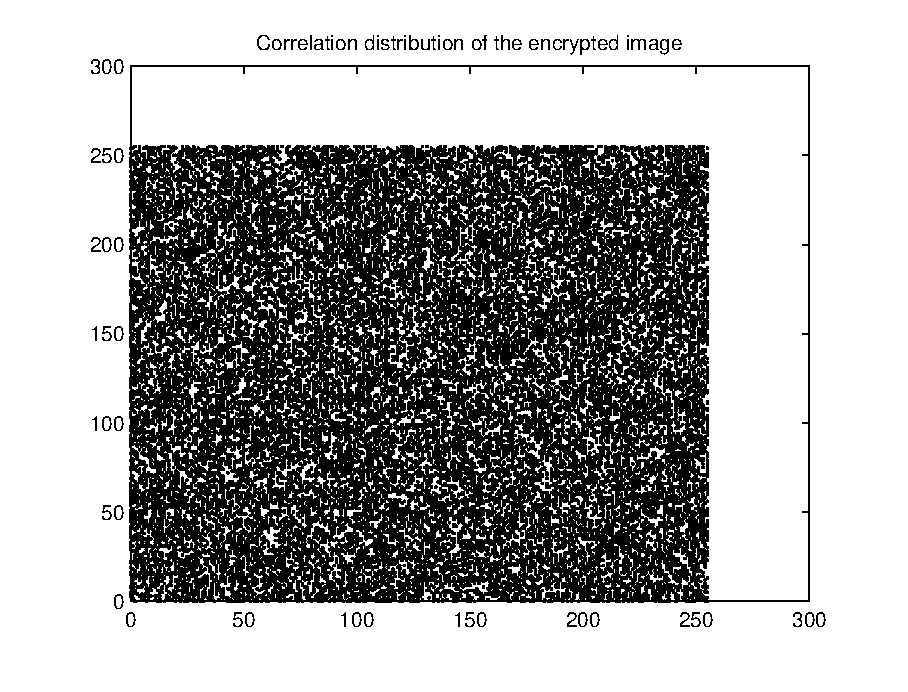
\includegraphics[scale = 0.35]{cd_old_ci.eps} %[Histogram of digitized laser]
}
\caption{(a) The encrypted Lena (one-time pad using Version 1 CI). (b) Histogram of Fig.(a). (c) Correlation distribution of two adjacent pixels in Fig.(a)}
\label{Old_CI}
\end{figure*}
%
\begin{figure*}
\centering
\subfigure[]{
\includegraphics[scale = 0.55]{lena_crypt_new_ci.eps} %[Histogram of digitized laser]
}
\subfigure[]{\includegraphics[scale = 0.35]{hist_new_ci.eps} %[Histogram of digitized laser]
}
\subfigure[]{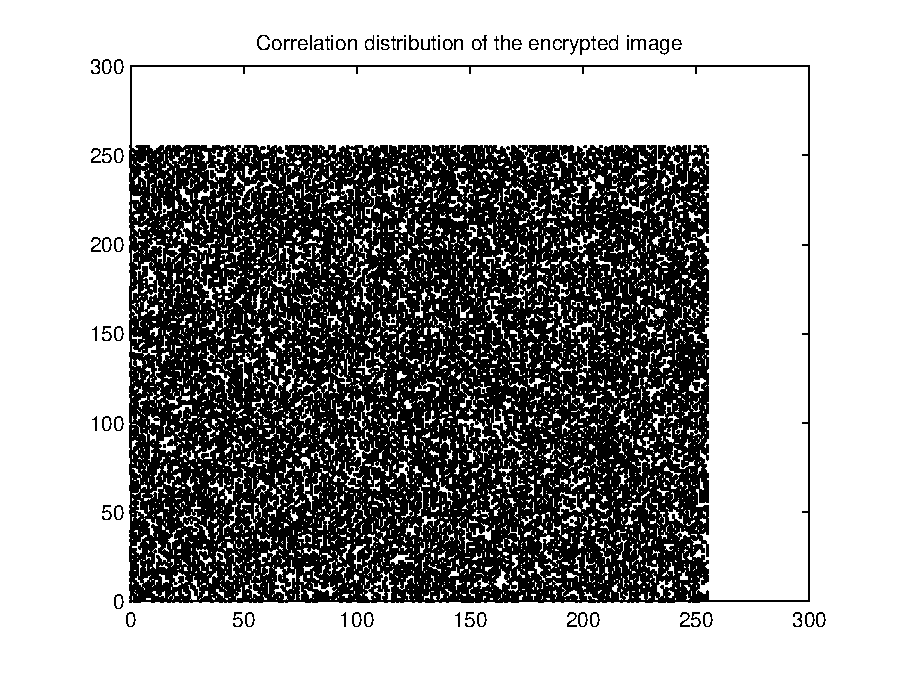
\includegraphics[scale = 0.35]{cd_new_ci.eps} %[Histogram of digitized laser]
}
\caption{(a) The encrypted Lena (one-time pad using Version 2 CI). (b) Histogram of Fig.(a). (c) Correlation distribution of two adjacent pixels in Fig.(a)}
\label{New_CI}
\end{figure*}
%Recent years, some researchers have investigated with success the use of chaotic dynamical systems to generate pseudorandom sequences~\cite{Hu20092286, DeMicco20083373}.
%Indeed, chaotic systems have many advantages as unpredictability or disorder-like, which are needed when producing complex sequences.
%They are extremely sensitive to the initial states too: a minute difference can cause a significant change in output.
%All these features fit well the requirements of PRNGs, thus explaining the proposal of such dynamics
%to secure exchanges.
%However, chaotic systems using real numbers on infinite bit representation, realized in finite computing precision, lead to short cycle length, non-ideal distribution, and other deflation of this kind.
%This is why chaotic systems on a infinite space of integers have been dig for these years, leading to the proposition to use chaotic iterations (CIs) techniques to reach the desired goals.
\begin{figure*}
\centering
\subfigure[]{\includegraphics[scale = 0.29]{hist_old_ci.eps} %[Histogram of digitized laser]
}
\subfigure[]{\includegraphics[scale = 0.29]{hist_old_ci_info.eps} %[Histogram of digitized laser]
}
\subfigure[]{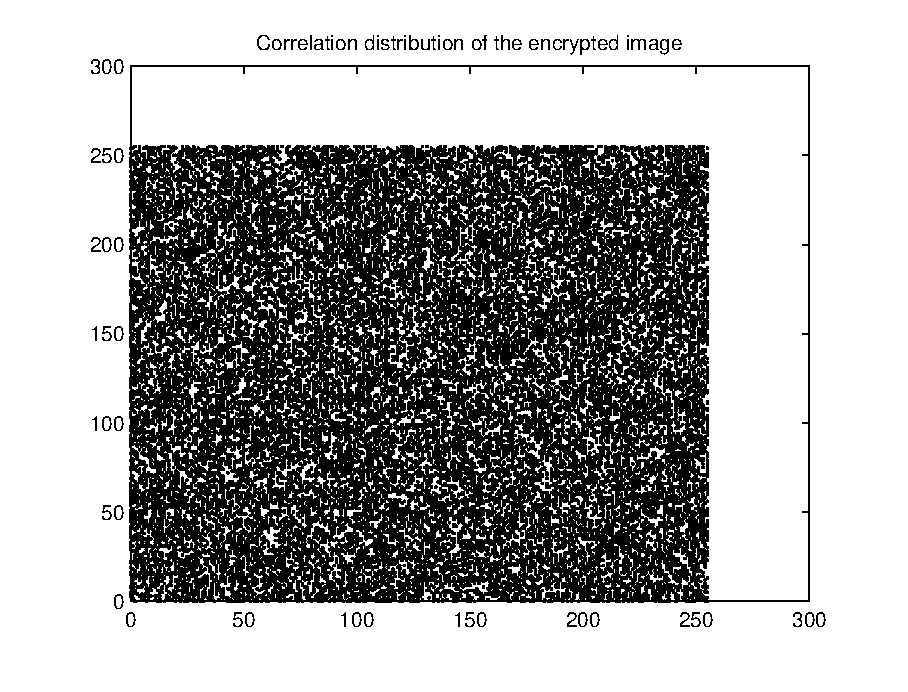
\includegraphics[scale = 0.29]{cd_old_ci.eps} %[Histogram of digitized laser]
}
\subfigure[]{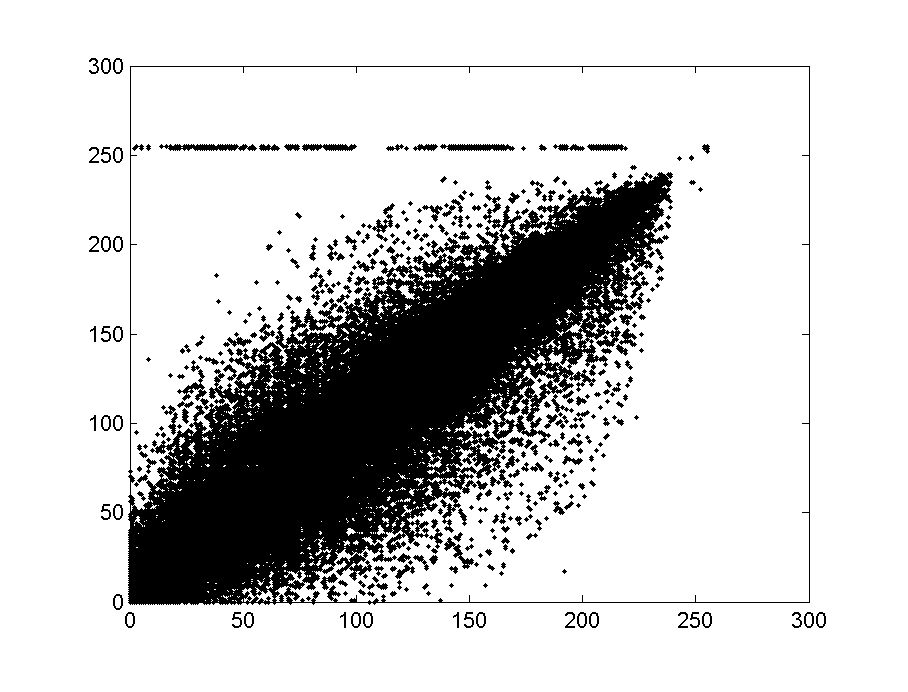
\includegraphics[scale = 0.29]{cd_old_ci_info.eps} %[Histogram of digitized laser]
}
\caption{ (a) Histogram of pixel values when LSBs are replaced by Version 1 CI. (b) Histogram of pixel values when LBSs are an hidden message xored with Version 1 CI. (c) Correlation distribution of two adjacent pixels in Fig.(a). (d) Correlation distribution of two adjacent pixels in Fig.(b).  }
\label{Old_CI_hiding}
\end{figure*}
\begin{figure*}
\centering
\subfigure[]{\includegraphics[scale = 0.29]{hist_new_ci.eps} %[Histogram of digitized laser]
}
\subfigure[]{\includegraphics[scale = 0.29]{hist_new_ci_info.eps} %[Histogram of digitized laser]
}
\subfigure[]{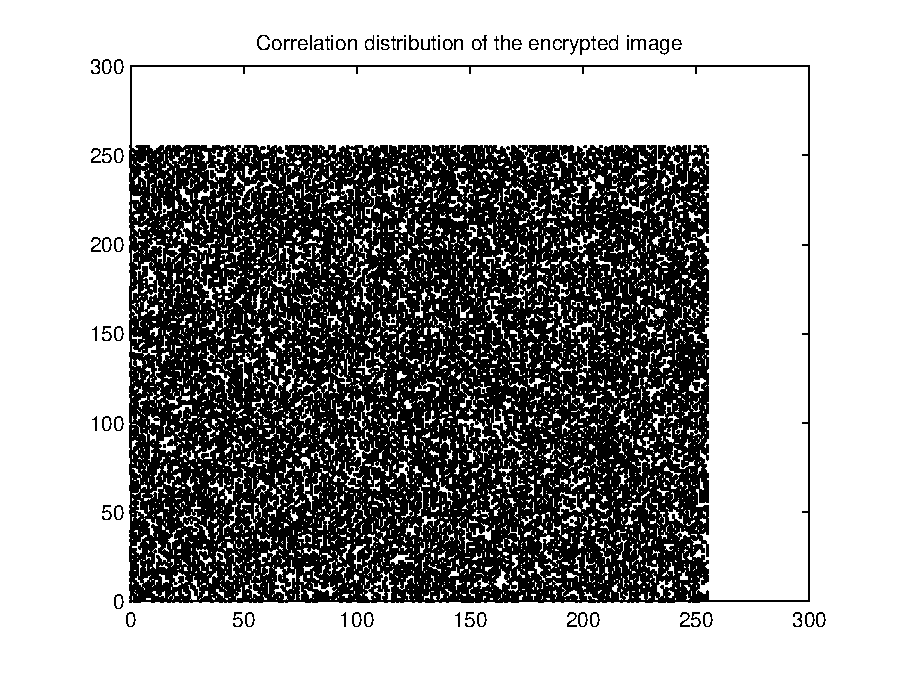
\includegraphics[scale = 0.29]{cd_new_ci.eps} %[Histogram of digitized laser]
}
\subfigure[]{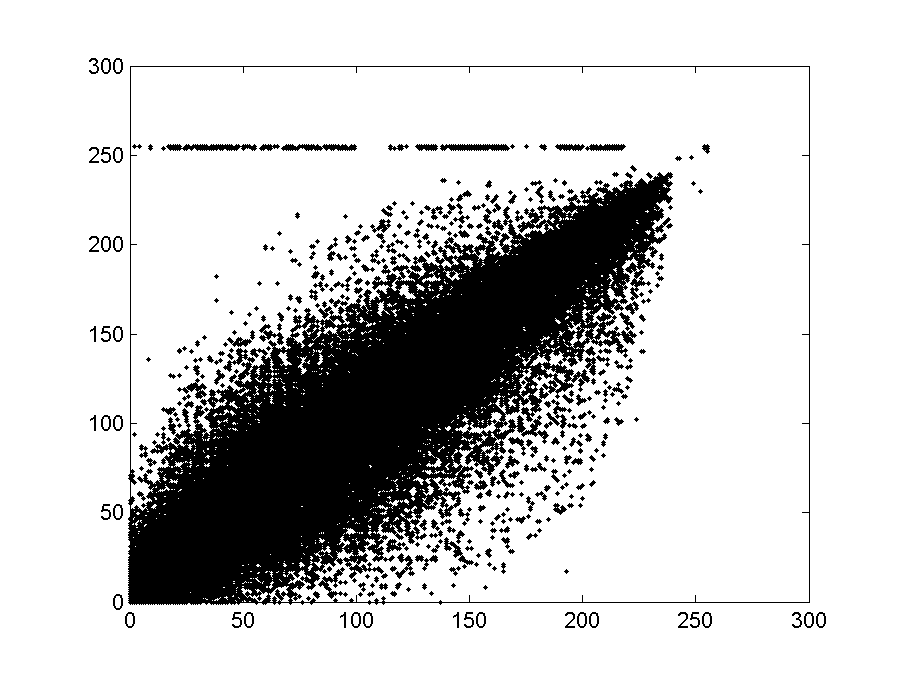
\includegraphics[scale = 0.29]{cd_new_ci_info.eps} %[Histogram of digitized laser]
}
\caption{ (a) Histogram of pixel values when LSBs are replaced by Version 2 CI. (b) Histogram of pixel values when LBSs are an hidden message xored with Version 2 CI. (c) Correlation distribution of two adjacent pixels in Fig.(a). (d) Correlation distribution of two adjacent pixels in Fig.(b).  }
\label{New_CI_hiding}
\end{figure*}
%The objective of this chapter is to make a state-of-the-art of chaotic iterations-based PRNGs, and to propose a possible use of them in the field of secrecy preservation through the Internet,
%by using information hiding techniques.
Random binary sequences will be generated by the three first CIPRNG methods using a XORshift generator.
The application of these pseudorandom bits for information hiding will be carried out systematically, and results will be discussed in order to verify that an attacker, who has only access to some elementary statistical tests,
cannot determine whether hidden information are embedded into cover documents or not.
Notice that the aim of this chapter is not to propose an up-to-date, finalized,
and secure data hiding scheme, but only to show the usability and effectiveness 
of our CIPRNGs.

\section{Application Evaluation}
\label{sec:application}

Let us firstly introduce our toy example in the information hiding security field. 

\subsection{The Proposed Information Hiding Method}

\begin{figure*}
\centering
\subfigure[]{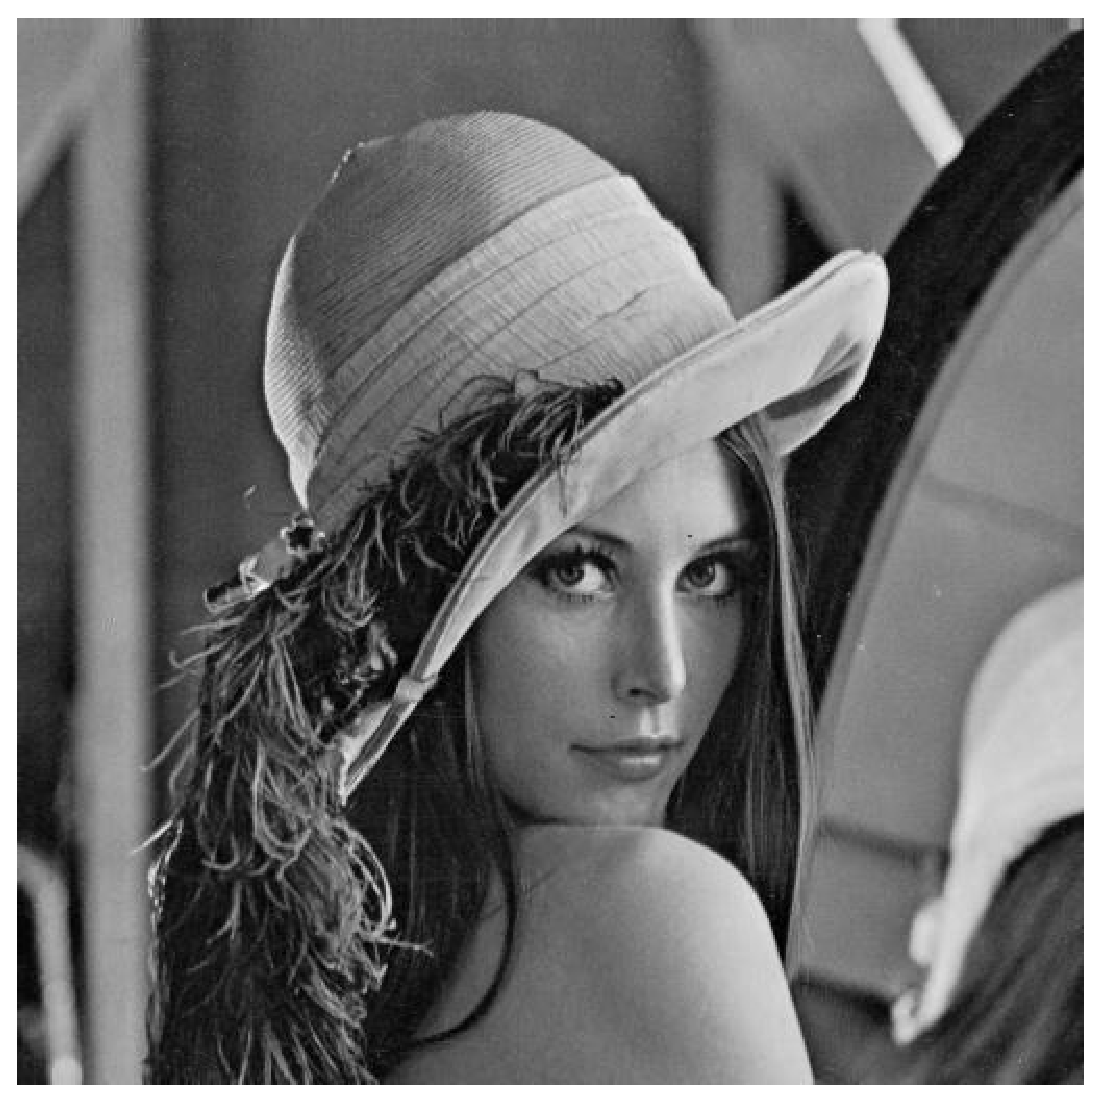
\includegraphics[scale = 0.15]{lena512.eps} %[Histogram of digitized laser]
}
\subfigure[]{
\includegraphics[scale = 0.35]{invader1.eps} %[Histogram of digitized laser]
}
\subfigure[]{\includegraphics[scale = 0.35]{hist_lena.eps} %[Histogram of digitized laser]
}
\subfigure[]{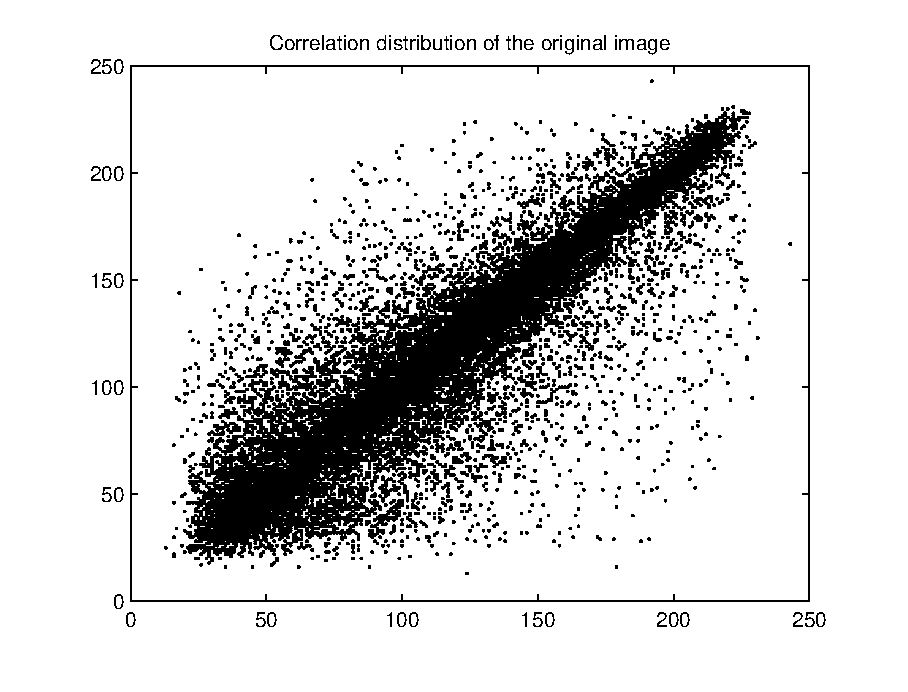
\includegraphics[scale = 0.35]{cd_lena.eps} %[Histogram of digitized laser]
}

\caption{(a) The original image. (b) The hidden image. (c) Correlation distribution of the original image. (d) Histogram of the original image.}
\label{Original}
\end{figure*}

Suppose that the size of the image is $M \times N$. The steps of the proposed information hiding
algorithm using the CIPRNG family (versions 1-3) are summed up below. Researches presented in this chapter have been formerly submitted/accepted/published in \cite{bfg12b:ip}.
\begin{enumerate}
\item Generate a pseudorandom sequence $S$ of length $M \times N$  using each CIPRNG method respectively.
\item Transform the image into a $M \times N$ integer sequence.
\item The LSBs (Least Significant Bits) of the image integer sequence are replaced by the generated random bits $S$. These random LSBs will be treated as a keystream.
\item The information (text or picture) to hide is transformed into a binary sequence.
\item The binary message is hiding into the random LSBs of the image sequence, by using the bitwise exclusive or operation between the two sequences, starting from a selected position acting as part of the secret key.
\end{enumerate}

As mentioned previously, pseudorandom sequences generated by the three CI methods, with two XORshift generators and a given image, are used in this application to process to an evaluation of the scheme.

\subsection{First Experimental Evaluation of the Proposed Scheme}

\subsubsection{The context}

The original image of size $713 \times 713$,
probably the most widely used test image for all kind of processing algorithms (such as compression and encryption),
 is depicted in Fig.~\ref{Original}-a.
Fig.~\ref{Original}-c presents its histogram, and Fig.~\ref{Original}-d shows the correlation distribution of two horizontal adjacent pixels in this original image.
Finally, information that must be hidden into it is the picture of Fig.~\ref{Original}-b, which has $89 \times 89$ pixels.

\begin{figure*}
\centering
\subfigure[]{
\includegraphics[scale = 0.55]{xor_ci_new.eps} %[Histogram of digitized laser]
}
\subfigure[]{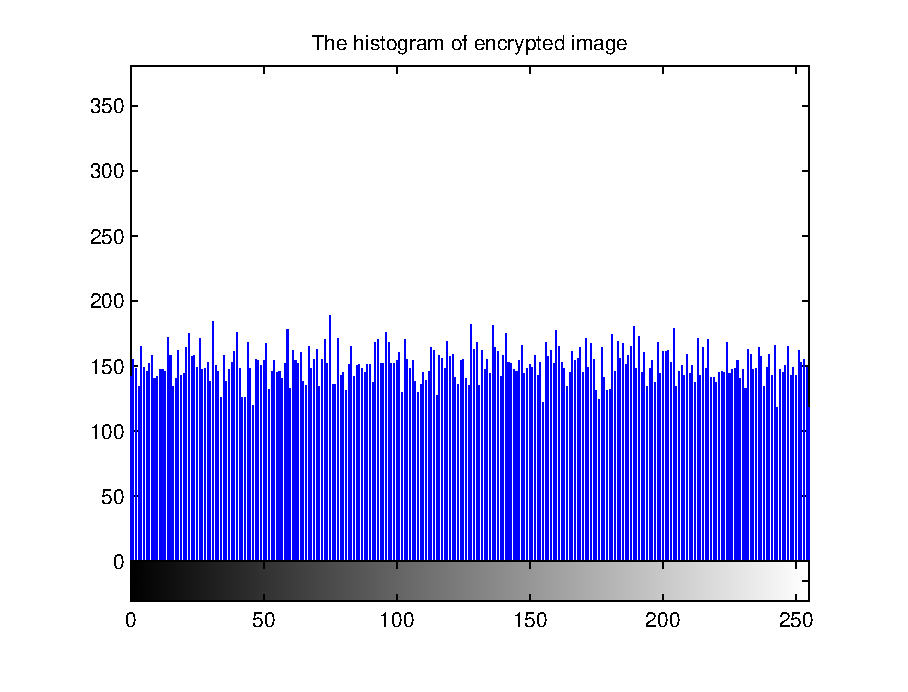
\includegraphics[scale = 0.35]{hist_xor_ci.eps} %[Histogram of digitized laser]
}
\subfigure[]{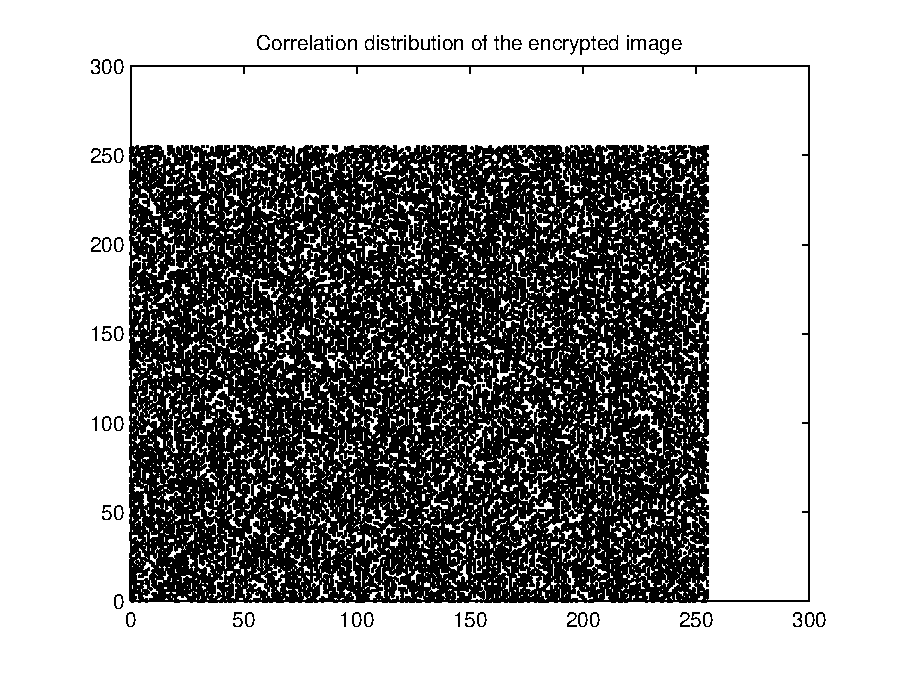
\includegraphics[scale = 0.35]{cd_xor_ci.eps} %[Histogram of digitized laser]
}
\caption{(a) The encrypted Lena (one-time pad using Version 3 CI). (b) Histogram of Fig.(a). (c) Correlation distribution of two adjacent pixels in Fig.(a)}
\label{Xor_CI}
\end{figure*}


\begin{figure*}
\centering
\subfigure[]{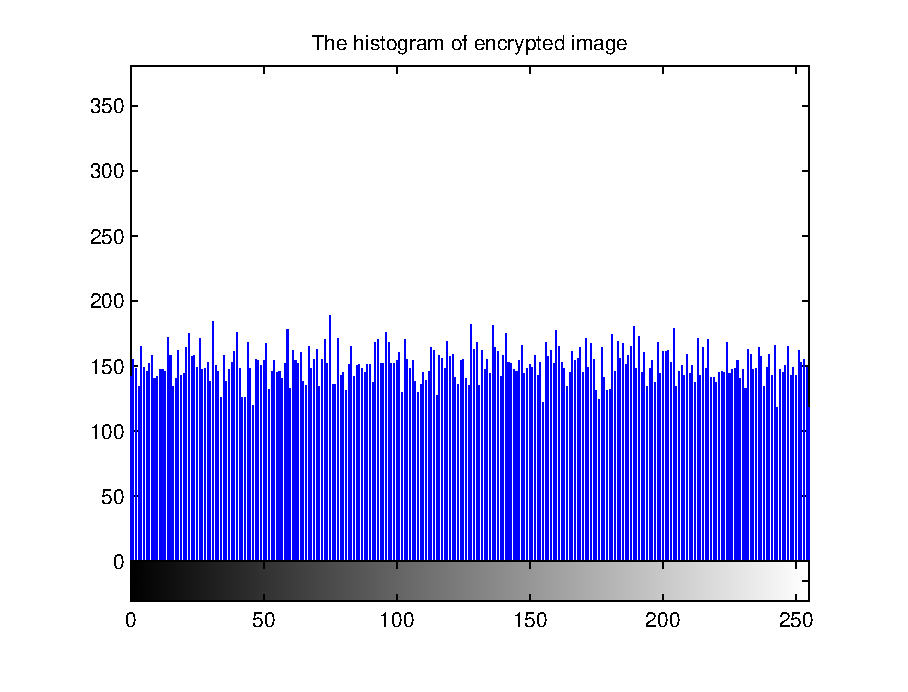
\includegraphics[scale = 0.29]{hist_xor_ci.eps} %[Histogram of digitized laser]
}
\subfigure[]{\includegraphics[scale = 0.29]{hist_xor_ci_info.eps} %[Histogram of digitized laser]
}
\subfigure[]{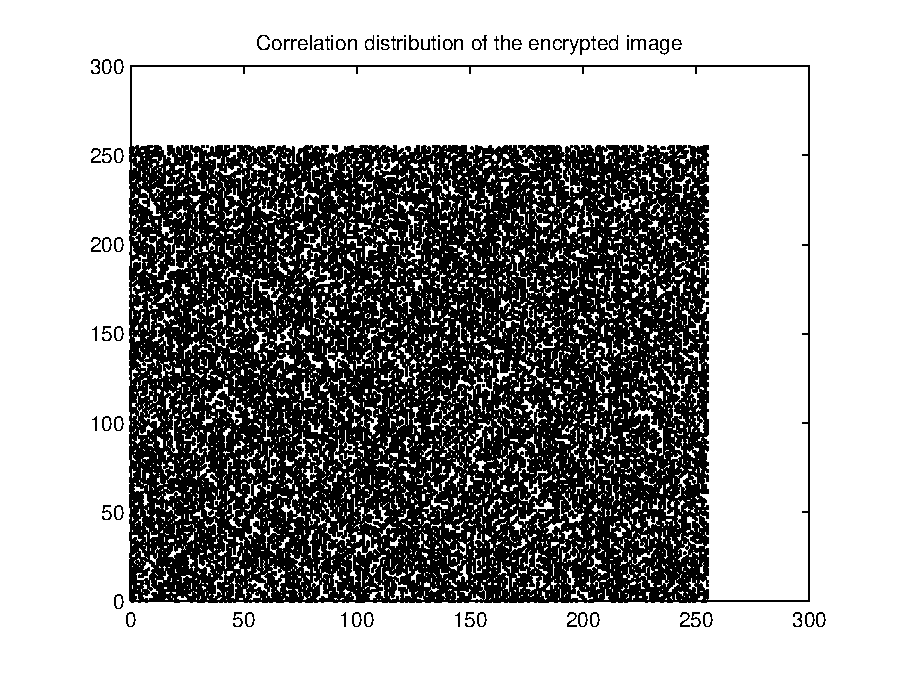
\includegraphics[scale = 0.29]{cd_xor_ci.eps} %[Histogram of digitized laser]
}
\subfigure[]{\includegraphics[scale = 0.29]{cd_xor_ci_info.eps} %[Histogram of digitized laser]
}
%\caption{ (a) Histogram of the random LSBs image using Version 3 CI. (b) Histogram of the random LSBs image using Version 3 CI with information hiding. (c) Correlation distribution of the random LSBs image using Version 3 CI. (d) Correlation distribution of the random LSBs image using Version 3 CI with information hiding.  }
\caption{ (a) Histogram of pixel values when LSBs are replaced by Version 3 CI. (b) Histogram of pixel values when LBSs are a hidden message xored with Version 3 CI. (c) Correlation distribution of two adjacent pixels in Fig.(a). (d) Correlation distribution of two adjacent pixels in Fig.(b).  }

\label{Xor_CI_hiding}
\end{figure*}


\subsubsection{Histogram and Horizontal Correlation}

Two XORshift generators are used to generate a random sequence based on the Version 1 CI method. Results are shown in Fig.~\ref{Old_CI_hiding}. Histograms and correlation distributions (Fig.~\ref{Old_CI_hiding}-a,b,c,d) are very closed to each other, leading to the
assumption that such a method can well protect the hidden information when facing statistical attacks.
The same experimental validation has been applied to the Version 2 CI method using two XORshift generators.
Such experiments lead to results that are shown in Fig.~\ref{New_CI_hiding}. These first results are
encouraging and confirm that simple histogram
and correlation evaluations cannot detect the
presence of hidden messages.
The same conclusion can be claimed when using the Version 3 CI generator, as it is depicted in Fig.~\ref{Xor_CI_hiding}.

%\subsubsection{Encryption with Version 3 CI}


\begin{figure*}
\centering
\subfigure[]{
\includegraphics[scale = 0.15]{diff_old_ci.eps} %[Histogram of digitized laser]
}
\subfigure[]{
\includegraphics[scale = 0.15]{diff_new_ci.eps} %[Histogram of digitized laser]
}
\subfigure[]{
\includegraphics[scale = 0.15]{diff_xor_ci.eps} %[Histogram of digitized laser]
}
\caption{(a) The difference of two random LSBs image using Version 1 CI PRNG with slight change in initial condition. (b) The difference of two random LSBs image using Version 2 CI PRNG with slight change in initial condition (c) The difference of two random LSBs image using Version 3 CI PRNG with slight change in initial condition}
\label{diff}
\end{figure*}


\begin{table*}
\centering
\renewcommand{\arraystretch}{1.3}
\caption{Correlation coefficients of two adjacent pixels in all directions in the original image, random LSBs images and infomation intergraded random LSBs images}
\label{coefficients}
\centering
  \begin{tabular}{|l||c|c|c|}
    \hline
\backslashbox{\textbf{Image}} {\textbf{Direction}} & Horizontal & Vertical & Diagonal \\ \hline
 Original image& 0.9793& 0.9686& 0.9488 \\ \hline
 Version 1 CI  \\\hline
 no info &0.9792& 0.9686& 0.9488 \\ \hline
 intergrading info& 0.9792& 0.9686& 0.9488 \\ \hline
 Version 2 CI  \\\hline
 no info & 0.9793& 0.9686& 0.9488 \\ \hline
 intergrading info & 0.9793& 0.9686& 0.9488  \\ \hline
 Version 3 CI \\ \hline
 no info& 0.9793& 0.9686& 0.9487 \\ \hline
 intergrading info& 0.9793& 0.9686& 0.9487 \\ \hline
\end{tabular}
\end{table*}

\subsubsection{All directions correlation coefficients analysis}

Using an identical experimental evaluation than in~\cite{Chen2004749}, the correlation coefficients of the horizontal, vertical, and diagonal directions of all the concerned images (original, with random as LSBs, and with secret information in these LSBs) are shown in Table~\ref{coefficients}.
It can be experimentally deduced that the correlation properties of these images are very similar to each other.
So an attacker, whose intention is to analyze
these coefficients in order to detect possible
information hiding, cannot attain his/her goal
by such a simple experiment.

\subsubsection{Initial condition sensitivity}

One of the most important properties of the chaotic sequences is that they are very sensitive to their initial conditions.
This property can help to face an attacker who
has access to the whole algorithm and to an
approximation of the secret key.
His/her intention, in this attack scenario, is
to find the exact secret key (the seed of the
keystream and the position of the message), by
making small changes on this key.
If the keystream and the position do not change
a lot when the key is slightly updated, then the
attacker can converge by small changes to the used secret key.
In the experiments of Figure~\ref{diff}, we slightly alter the keys and try to extract the hidden information from the image.
We can conclude that such optimistic attempts
always fail in recovering the message.



\subsection{A small evaluation of Encryption}

The dissimulation has been obtained in this paper by using the CIPRNGs recalled previously as stream
cyphers:  encryption is the result of the use of the bitwise exclusive or (XOR) between the given message and pseudorandom sequences generated from various CIPRNGs. We can wonder whether an attacker, who has access
to the histogram of LSBs, can infer what kind of CIPRNG has been used as keystream.
For obvious reasons, these histograms should at least be uniform for each PRNG.

For illustration purpose, Lena has been encrypted by such method using each of the three kind of
CIPRNGs, and histogram and correlation distribution of the encrypted image have been computed. The resulting images are depicted in Fig.~\ref{Old_CI}
when using the Version 1 CI method, in Fig.~\ref{New_CI} for the Version 2 CI one, and in Fig.~\ref{Xor_CI} for the last PRNG recalled here.
We can show that this first reasonable requirement seems to be respected, even if this illustration
is not a proof.

\section{Conclusion}

We have %summarized in this chapter our previous contributions in the field of pseudorandom
%generators, and we have 
proposed, in this short application chapter, simple illustrative examples of use for information hiding.
The three first versions of the CIPRNGs family have been used here. 
%recalled here are namely the Version 1 CI, the Version 2 CI, and the Version 3 CI PRNGs.
For each generator,
firsts experimental evaluations of a simple information hiding scheme have been realized,
to illustrate that that an attacker using simple
statistics cannot determine easily, only by regarding the form of histograms or
 correlation distributions, the presence of an hidden message into a given document.
No evidence of dissimulation appears at first glance, when comparing histograms, correlation distribution, or all directions' correlation coefficients. Furthermore, experiments have illustrated high sensitivity to the secret parameters.
These simple evaluations do not imply the security of the proposed scheme, they only illustrate that the
use of the CIPRNGs for information hiding can be further investigated by more stringent tools
as steganalyzers and
mathematical proofs.

\chapter{FPGA Acceleration of CIPRNGs}
\label{FPGA Acceleration of CIPRNGs}

As well-designed information security 
applications frequently use a very large quantity of good 
pseudorandom numbers, inefficient generation of 
these numbers can be a significant bottleneck 
in various situations~\cite{Porter198443,Batina20031,Carroll1990613,Liu2012331}. 
%For the implementation of the general-purpose cryptanalysis devices
In that context, re-configurable hardware like field programmable gate arrays (FPGAs)
 have for many years been identified as a suitable technology having the potential to improve performance compared to traditional microprocessor based approaches. 
%Particularly,  were successfully applied that is a highly parallelizable task.

In this chapter, %In this new research work, 
our generators based on chaotic 
iterations are redesigned specifically for FPGA hardware, 
leading to an obvious improvement of the 
generation rate of such numbers. Analyses illustrate that 
statistically perfect and chaotic random sequences 
are produced (and, as established previously, such 
generators can be cryptographically secure too).
The research has been submitted in \cite{submit1, submit3} before.

\section{introduction}
PRNGs are very important primitives widely used 
in numerous applications like numerical simulations or security.
%For instance, they are one of the most fundamental component that any 
%cryptosystem has to embed, in order to generate encryption keys or keystreams
%in symmetric ciphers. 
Depending on the targeted application, these PRNGs must achieve requirements
as speed, statistical quality, security, and so on. 
On the one hand, field programmable gate arrays (FPGAs) have been successfully used for realizing 
the speed requirement in pseudorandom sequence generation, due to their high parallelization capability \cite{Bojani200663, Danger:2009:HST:1645457.1645933, Tsoi:2003:CFT:938383.938400}. Advantages of such physical generation way encompass performance, design time, power consumption, flexibility, and cost.


It has been stated in the previous chapters that chaotic iterations are
good candidates to generate  sequences both secure and random,
due among other things to
their sensitivity to initial conditions and their broadband spectrum. 
Our intention in this chapter, which continues the studies initiated 
in~\cite{DBLP:journals/corr/abs-1112-5239}, is to merge these two approaches by
proposing a discrete chaos-based generator
designed on FPGA.

\section{CIPRNG design on FPGA}
\label{FPGA design}
\subsection{Selection of the CIPRNG version}

According to the comparison produced in Chapter~\ref{Statistical Tests for Randomness}, 
it can be seen that CIPRNG version 4 is the most adaptable of all the generators into
this chaotic iterations based family. 
The loop processing that he embeds can be replaced by parallel computing to increase  efficiency. 
Let us recall that the CIPRNGs used here are both proven to be cryptographically secure (see Section~\ref{Security Analysis}) due to the use of a BBS (and three XORshift PRNGs), 
and its statistical performance are good enough to pass with success the NIST, DieHARD, and TestU01 test suites (see Section~\ref{test for Version 4 CI}).

In order to take benefits from the computing power of FPGA, a whole processing
needs to spread the various components of the generator 
into several independent blocks  of threads that can be computed
simultaneously. In general,  the larger the number of  threads is, the
more logistic elements of FPGA are used, and the less branching  instructions are
used  (if,  while,  ...),  the  better the  performances  on  FPGA  are.
Obviously, having these requirements in  mind, it is possible to build
a program similar to the algorithm presented in Tab.
\ref{fpga ci}, which produces pseudorandom numbers with chaotic properties on FPGA.  
To do so,  Verilog-HDL~\cite{verilog} has been used to help programing. 
In this generator, there are three
PRNG objects that use the exclusive or operation, two XORshifts, and a BBS, 
their processing are described thereafter.


\subsection{Design of XORshift}

The structure of XORshift designed in Verilog-HDL is shown in Fig.\ref{xorshift verilog}. There are four inputs:
\begin{itemize}
\item The first one is the initial state, which costs 64 bits 
of register units,
\item the other three ones are used to define the shift operations.
\end{itemize}
Let us remark that, in FPGA, this shift operation costs nothing,
as it simply consists in using different bit cells of the input. 
We can thus conclude that there are $64 - s1 + 64 -s2 + 64 -s3 
= 192 - s1 - s2 - s3$ logic gates elements that are required for
the XORshifts processing. 
\begin{figure}
\begin{center}
  \subfigure[XORshift]{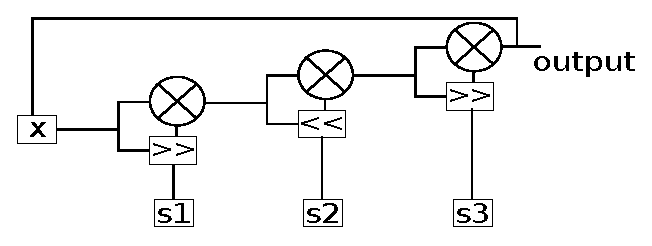
\includegraphics[width=6.5cm]{xorshift.eps}
  \label{xorshift verilog}}
  \subfigure[BBS]{\includegraphics[width=6.5cm]{bbs.eps}
  \label{BBS verilog}}
  \subfigure[The proposed CIPRNG]{\includegraphics[width=10cm]{ci.eps}
  \label{CI verilog}}
\end{center}
\caption{The processing structure for BBS in FPGA (per clock step)}
\end{figure}
%In our program, we define 
%each FPGA clock positive edge, the XORshift will work, since these are simple processing for FPGA, every 
%clock step can lead to one output.

\subsection{Design of BBS}
Fig.\ref{BBS verilog} gives the proposed design of the BBS generator in FPGAs.
There are two inputs of $32$ bits, namely 
$b$ and $m$. 
Register $b$ stores the state of the system
at each time (after the square computation). 
$m$ is also a register that saves the value of $M$, which must not change.
Another register $b\_extend$ 
is used to combine $b$ to a data having $64$ bits, with a view to avoid overflow. 
After the last computation,
the three LSBs from the output of $\%$ are
taken as output. 
Let us notice that a BBS is
 performed at each time unit.

\begin{figure}
\begin{center}
  \includegraphics[width=6.5cm]{print.eps}
\end{center}
\caption{The sources cost in $EP2C8Q208C8$ FPGA board}
 \label{logic elements}
\end{figure}

\subsection{Design of the chaotic iterations}
Two XORshifts and one BBS are connected to work together, in order to compose the
proposed CIPRNG (see Fig.\ref{CI verilog}). 
As it can be shown, the three bits of the BBS output are switches for the corresponding $32$ bits XORshift outputs. Every round of the 
 processing costs two time units
 to be performed: in the first clock, 
the four PRNGs are processed in parallel,
whereas in the second one, the results of these generators are combined with 
the current state of the system, in order to produce the output of $32$ bits. 

In our experiments, the type $EP2C8Q208C8$ from Altera 
company's CYCLONE II FPGA series 
has been used. By default, its working
frequency is equal to $50$ MHz.
However, it is possible to increase it until
$400$ MHz by using the phase-lock loop (PLL) device.
In that situation, the CIPRNG designed on this
FPGA can produce about $6400$ Mbits per second
(that is, $400 (MHz) \div 2 (times) \times 32 (bits)$),
while using $3652$ of the $8256$ logic 
elements in $EP2C8Q208C8$ (see
Fig.\ref{logic elements}). 

In the next section, an application of this 
CSPRNG designed on FPGA in the information 
hiding security fields is detailed, to show
that this hardware pseudorandom generator 
is ready to use.

\chapter{Software and Hardware Implementation of a Watermarking Scheme using CIPRNG}
\label{Application Example}
\minitoc



%Cryptographically secure PRNGs are fundamental tools to communicate through the Internet. Original and encrypted image are shown in Fig.\ref{Distribution of original image}(a) and 
%Fig.\ref{Distribution of encrypted image}(a), whereas Fig.\ref{Distribution of original image}(b) and Fig.\ref{Distribution of encrypted image}(b) depict their histograms. 
%Obviously the distribution of the encrypted image is very close to the uniform distribution, which improves the protection against statistical attacks.
%
%
%
%
%
%\begin{figure*}
%\begin{minipage}[b]{.48\linewidth}
%\centering
%\centerline{\epsfig{figure=lena.eps,width=5cm}}
%\centerline{(a) Original image.}
%\end{minipage}
%\hfill
%\begin{minipage}[b]{0.48\linewidth}
%\centering
%\centerline{\epsfig{figure=Histogram_lena.eps,width=8cm}}
%\centerline{(b) Histogram.}
%\end{minipage}
%\caption{Distribution of original image}
%\label{Distribution of original image}
%\end{figure*}
%
%\begin{figure*}
%\begin{minipage}[b]{.48\linewidth}
%\centering
%\centerline{\epsfig{figure=lena_crypt.eps,width=5cm}}
%\centerline{(a) Encrypted image.}
%\end{minipage}
%\hfill
%\begin{minipage}[b]{0.48\linewidth}
%\centering
%\centerline{\epsfig{figure=Histogram_lena_crypt.eps,width=8cm}}
%\centerline{(b) Histogram.}
%\end{minipage}
%\caption{Distribution of encrypted image}
%\label{Distribution of encrypted image}
%\end{figure*}
%
%Fig.\ref{Correlation distributions of two horizontally adjacent pixels in the original image and the encrypted image} shows the correlation distribution of two horizontally adjacent pixels, both in the original and in the encrypted images. Correlation coefficients in the horizontal, vertical, and diagonal directions concerning these two images are presented in Tab.\ref{Correlation coefficients of two adjacent pixels in the original image and the encrypted image}. Obviously, the correlation is important in the original image, whereas it is low and can be ignored in the encrypted image. These simple illustrations tend to prove that the use of CI PRNGs for cryptographic applications can be studied, to determine whether these chaotic generators is cryptographically secure working at the application or not. These study has been partially initiated in \cite{guyeuxTaiwan10,bgw10:ip,bfgw11:ij,bfg12b:ip}, in which our generators have been used as a component of watermarking scheme. The robustness of this scheme 
%has been evaluated, which has led to results as good as possible, thus reinforcing our opinion that these generators would probably be useful in cryptographic applications.
%The question of whether CI PRNGs are working application well or not, will thus be raised in our next work.
%
%\begin{figure*}
%\begin{minipage}[b]{.48\linewidth}
%\centering
%\centerline{\epsfig{figure=Correlation_distribution_of_the_original_image.eps,width=8cm}}
%\centerline{(a) Original image.}
%\end{minipage}
%\hfill
%\begin{minipage}[b]{0.48\linewidth}
%\centering
%\centerline{\epsfig{figure=Correlation_distribution_of_the_encrypted_image.eps,width=8cm}}
%\centerline{(b) Encrypted image.}
%\end{minipage}
%\caption{Correlation distributions of two horizontally adjacent pixels}
%\label{Correlation distributions of two horizontally adjacent pixels in the original image and the encrypted image}
%\end{figure*}
%
%\begin{table*}
%\renewcommand{\arraystretch}{1.3}
%\caption{Correlation coefficients of two adjacent pixels in the original image and the encrypted image}
%\label{Correlation coefficients of two adjacent pixels in the original image and the encrypted image}
%\centering
%\begin{tabular}{ccc} \toprule
%\textbf{Direction} &\textbf{Original image} & \textbf{Encrypted image} \\ \midrule
%Horizontal &0.9245 &-0.0059 \\
%Vertical &0.9617 &-0.0048 \\
%Diagonal &0.8967 &-0.0052 \\ \bottomrule
%\end{tabular}
%\end{table*}


\section{Introduction}

As stated in a previous chapter, information hiding has recently become a major information security technology, 
especially with the increasing importance and widespread distribution of digital media 
through the Internet \cite{Wu2007bis}. It includes several techniques like digital watermarking. 
The aim of digital watermarking is to embed a piece of information into digital documents, such as pictures 
or movies. This is for a large panel of reasons, such as: copyright protection, control utilization, data description,
content authentication, and data integrity. For these reasons, many different watermarking schemes have been proposed in 
recent years. 

Digital watermarking must have essential characteristics, including: security, imperceptibility, and robustness.
Chaotic methods have been proposed to encrypt the watermark before embedding it in the carrier image for these security reasons. % Idem
In this section, a watermarking algorithm based on the chaotic PRNGs presented in this part is given, as an 
illustration of use of these PRNG based on CIs \cite{submit2, bibtexwangqianxue}.

\section{Definition of our Chaos-Based Information Hiding Scheme}
\label{sec:Algo}

Let us now introduce a more complex information hiding scheme based on chaotic iterations.
It has been formerly introduced in~\cite{gfb10:ip,bg10:ip}, in which more complete 
explanations on details of the
proposed scheme can be found.


\subsection{Most and least significant coefficients}

Let us define the notions of most and least significant coefficients of an image.

\begin{Definition}
\label{definitionMSC}
For a given image, most significant coefficients (in short MSCs), are coefficients that allow the description of the relevant part of the image, \emph{i.e.}, its richest part (in terms of embedding information), through a sequence of bits.
\end{Definition}

For example, in a spatial description of a grayscale image, a definition of MSCs can be the sequence constituted by the first four bits of each pixel (see Figure~\ref{fig:MSCLC}). In a discrete cosine frequency domain description, each $8\times 8$ block of the carrier image is mapped onto a list of 64 coefficients. The energy of the image is mostly contained in a determined part of themselves, which can constitute a possible sequence of MSCs.

\begin{Definition}
\label{definitionLSC}
By least significant coefficients (LSCs), we mean a translation of some insignificant parts of a medium in a sequence of bits (insignificant can be understand as: ``which can be altered without sensitive damages'').
\end{Definition}

These LSCs can be, for example, the last three bits of the gray level of each pixel (see Figure~\ref{fig:MSCLC}). Discrete cosine, Fourier, and wavelet transforms can be used also to generate LSCs and MSCs. Moreover, these definitions can be extended to other types of media.




\begin{figure}[htb]

\begin{minipage}[b]{1.0\linewidth}
  \centering
 \centerline{\epsfig{figure=lena512.eps,width=4cm}}
  \centerline{(a) Lena.}
\end{minipage}

\begin{minipage}[b]{.48\linewidth}
  \centering
 \centerline{\epsfig{figure=lena_msb_678.eps,width=4cm}}
  \centerline{(b) MSCs of Lena.}
\end{minipage}
\hfill
\begin{minipage}[b]{0.48\linewidth}
  \centering
 \centerline{\epsfig{figure=lena_lsb_1234_facteur17.eps,width=4cm}}
  \centerline{(c) LSCs of Lena ($\times 17$).}
\end{minipage}
%
\caption{Example of most and least significant coefficients of Lena.}
\label{fig:MSCLC}
%
\end{figure}


LSCs are used during the embedding stage. Indeed, some of the least significant coefficients of the carrier image will be chaotically chosen by using our PRNG. These bits will be either switched or replaced by the bits of the watermark. The MSCs are only useful in case of authentication; mixture and embedding stages depend on them. Hence, a coefficient should not be defined at the same time as a MSC and a LSC: the last can be altered while the first is needed to extract the watermark.
\subsection{Stages of the scheme}

Our CIPRNG version 4 generator-based information hiding scheme consists of two stages: (1) mixture of the watermark and (2) its embedding.

\subsubsection{Watermark mixture}

Firstly, for security reasons, the watermark can be mixed before its embedding into the image. A first way to achieve this stage is to apply the bitwise exclusive or (XOR) between the watermark and the CIPRNG version 4. In this paper, we introduce a new mixture scheme based on chaotic iterations. Its chaotic strategy, which depends on our PRNG, will be highly sensitive to the MSCs, in the case of an authenticated watermarking.%For the detail of this stage see Sections \ref{Geometric} below.

\subsubsection{Watermark embedding}

Some LSCs will be switched, or substituted by the bits of the possibly mixed watermark. To choose the sequence of LSCs to be altered, a number of integers, less than or equal to the number $\mathsf{M}$ of LSCs corresponding to a chaotic sequence $U$, is generated from the chaotic strategy used in the mixture stage. Thus, the $U^{k}$-th least significant coefficient of the carrier image is either switched, or substituted by the $k^{th}$ bit of the possibly mixed watermark. In case of authentication, such a procedure leads to a choice of the LSCs which are highly dependent on the MSCs~\cite{guyeux10}.

On the one hand, when the switch is chosen, the watermarked image is obtained from the original image whose LSBs $L = \mathds{B}^{\mathsf{M}}$ are replaced by the result of some chaotic iterations. Here, the iterate function is the vectorial boolean negation,
\begin{equation}
f_0:(x_1,...,x_\mathsf{M}) \in \mathds{B}^\mathsf{M} \longmapsto (\overline{x_1},...,\overline{x_\mathsf{M}}) \in \mathds{B}^\mathsf{M},
\end{equation}
the initial state is $L$, and the strategy is equal to $U$. In this case, the whole embedding stage satisfies the topological chaos properties~\cite{guyeux10}, but the original medium is required to extract the watermark. On the other hand, when the selected LSCs are substituted by the watermark, its extraction can be done without the original cover (blind watermarking). In this case, the selection of LSBs still remains chaotic because of the use of the CIPRNG version 4, but the whole process does not satisfy topological chaos~\cite{guyeux10}. The use of chaotic iterations is reduced to the mixture of the watermark. See the following sections for more detail.

\subsubsection{Extraction}

The chaotic strategy can be regenerated even in the case of an authenticated watermarking, because the MSCs have not changed during the embedding stage. Thus, the few altered LSCs can be found, the mixed watermark can be rebuilt, and the original watermark can be obtained. In case of a switch, the result of the previous chaotic iterations on the watermarked image should be the original cover. The probability of being watermarked decreases when the number of differences increase.

If the watermarked image is attacked, then the MSCs will change. Consequently, in case of authentication and due to the high sensitivity of our PRNG, the LSCs designed to receive the watermark will be completely different. Hence, the result of the recovery will have no similarity with the original watermark.

The chaos-based data hiding scheme is summed up in Figure~\ref{fig:organigramme}.

\begin{figure}[htb]
\centerline{\epsfig{figure=organigramme22.eps,width=8.cm}}
\caption{The chaos-based data hiding decision tree.}
\label{fig:organigramme}
\end{figure}



\begin{figure}[h!]
\centering
\subfigure[Structure]{\includegraphics[width=6cm]{nios.eps}
\label{nios}} \hspace{0.5cm}
\subfigure[Schematic]{\includegraphics[width=\columnwidth]{nios2.eps}
\label{nios2}} \hspace{0.5cm}
\caption{NIOS II setting in FPGA}
\label{Spatial MSCs and LSCs of Lena}
\end{figure}

\section{Experimental protocol}
In this subsection, a concrete example is given: a watermark is encrypted and embedded into a cover image using the scheme presented in the previous section and  CIPRNG version 4 (BBS, XORshift). The carrier image is the well-known Lena, which is a 256 grayscale image, and the watermark is the $64\times 64$ pixels binary image depicted in Figure~\ref{Original images}.


\begin{figure}[!t]
\centering
\subfigure [The original image]{\includegraphics[scale=0.23]{lena512.eps}}
\hfil
\subfigure[The watermark]{\includegraphics[scale=0.4]{invader1.eps}%
}
\caption{Original images}
\label{Original images}
\end{figure}


\begin{figure}[!t]
\centering
\subfigure [Differences with the original]{\includegraphics[scale=0.42]{lenaDiff2.eps}%
}
\hfil
\subfigure [Encrypted watermark]{\includegraphics[scale=0.4]{invader_chiffre1.eps}%
}
\caption{Encrypted watermark and differences}
\label{Encrypted watermark and differences}
\end{figure}

The watermark is encrypted by using chaotic iterations: the initial state $x^{0}$ is the watermark, considered as a boolean vector, the iteration function is the vectorial logical negation, and the chaotic strategy $(S^{k})_{k\in \mathds{N}}$ is defined with CIPRNG version 4 (BBS, XORshift), where initial parameters constitute the secret key and $N=64$. Thus, the encrypted watermark is the last boolean vector generated by these chaotic iterations. An example of such an encryption is given in Figure~\ref{Encrypted watermark and differences}.


Let $L$ be the $256^3$ booleans vector constituted by the three last bits of each pixel of Lena and $U^k$ defined by the sequence:
\begin{equation}
\left\{
\begin{array}{lll}
U^{0} & = & S^{0} \\
U^{n+1} & = & S^{n+1}+2\times U^{n}+n ~ [mod ~ 256^3]%
\end{array}%
\right.
\end{equation}
The watermarked Lena $I_w$ is obtained from the original Lena, whose three last bits are replaced by the result of $64^2$ chaotic iterations with initial state $L$ and strategy $U$ (see Figure~\ref{Encrypted watermark and differences}).

The extraction of the watermark can be obtained in the same way. Remark that the map $\theta \mapsto 2\theta $ of the torus, which is the famous dyadic transformation (a well-known example of topological chaos~\cite{Dev89}), has been chosen to make $(U^{k})_{k \leqslant 64^2}$ highly sensitive to the strategy. As a consequence, $(U^{k})_{k \leqslant 64^2}$ is highly sensitive to the alteration of the image: any significant modification of the watermarked image will lead to a completely different extracted watermark, thus giving a way to authenticate media through the Internet.


Let us now evaluate the robustness of the proposed method.

\section{Implementations: from software to hardware}

We have been in charge to implement this chaotic iterations based watermarking
scheme on both software and hardware platforms, using one of the CIPRNGs we
previously studied. By doing so, we will be able to study the robustness
of the proposed hiding scheme, leading to the evaluation given in Section~\ref{robust}.

\subsection{Software Implementation: Experimental Protocol}

In this section, we details our software implementation of the information hiding application
 based on chaotic iterations presented in the previous sections: a watermark is encrypted and embedded into a cover image using the proposed scheme and some CIPRNGs. More precisely,
the CIPRNG(BBS, XORshift) version 4 has been chosen, since it is with good statistical performance and high efficiency.  The carrier image is the well-known Lena
already presented, which is here a $256 \times 256$ grayscale image, and the watermark is the $64\times 64$ pixels binary image depicted in Fig.\ref{Original images}.


\begin{figure}[!t]
\centering
\subfigure [The original image]{\includegraphics[scale=0.23]{lena512.eps}}
\hfil
\subfigure[The watermark]{\includegraphics[scale=0.4]{invader1.eps}%
}
\caption{Original images}
\label{Original images}
\end{figure}


\begin{figure}
\centering
\subfigure[Output image]{\includegraphics[scale=0.4]{output_lena.eps}}
\subfigure[Difference]{\includegraphics[scale=0.4]{diff.eps}}
\caption{The output of our watermarking application}
\label{java_end}
\end{figure}
The application has been computed using the JAVA language~\cite{java}. The watermark is encrypted by using chaotic iterations: the initial state $x^{0}$ is the watermark, considered as a Boolean vector, the iteration function is the vectorial logical negation, and the chaotic strategy $(S^{k})_{k\in \mathds{N}}$ is defined with CIPRNG(BBS, XORshift) version 4, whose initial parameters constitute the secret key and $N=64$.  
A simple windows interface has been implemented, as it is depicted in Fig.\ref{java application}-a.
The embedding file must firstly be chosen, as shown in Fig.\ref{java application}-b. 
Then the host image that will be used to carry the watermark must be selected (see Fig.\ref{java application}-c). Lastly, after processing, the output image is produced, and the differences between original image and encrypted image is produced (Fig.\ref{java_end}).

\begin{figure}
\centering
\subfigure [The start windows of our Java's watermarking application]{\includegraphics[scale=0.4]{start.eps}}
\subfigure [Choosing the contents to embed]{\includegraphics[scale=0.4]{chooseFile.eps}}
\subfigure [Choosing the contents to embed]{\includegraphics[scale=0.4]{chooseImage.eps}}
\caption{Java application for watermarking based on chaotic iterations}
\label{java application}
\end{figure}



\subsection{Hardware Implementation}

In this section, to show the effectiveness and lightweight of our approach using
chaotic iterations for both pseudorandom generations and information hiding,
we will shortly present our hardware implementation of the whole algorithm on a FPGA.
The 32-bit embedded-processor architecture designed specifically for the Altera family of FPGAs 
has been used for this application. Indeed, Nios II incorporates many enhancements over the original 
Nios architecture, making it more suitable for a wider range of embedded computing applications, 
from DSP to system-control, and to this watermarking scheme~\cite{nios}. 

Fig.\ref{nios} shows the structure of this application, 
the NIOS II system can read the image from the HOST computer side. 
Then the control bus allows
the CI generator to operate, in order to produce pseudorandom bits. 
Finally the processed results are transmitted back into 
the host. In Fig.\ref{nios2}, the NIOS II uses the most powerful 
version the CYCLONE II can support (that is, NIOS II/f). 
Then, $4$ KB on chip memory and $16$ MB SDRAM are set, and 
the $PLL$ device is used to enhance the clock frequency from $50$ 
to $200$ MHz. The data bus connects NIOS II system, and the generator is in 32 bits.


\section{Robustness evaluation}
\label{robust}
In what follows, the embedding domain is the spatial domain, CIPRNG(BBS,XORshift) version 4 
 has been used to encrypt the watermark, MSCs are the four first bits of each pixel (useful only in case of authentication), and LSCs are the three next bits.

To prove the efficiency and the robustness of the proposed algorithm, some
attacks are applied to our chaotic watermarked image. For each attack, a
similarity percentage with the watermark is computed, this percentage is the
number of equal bits between the original and the extracted watermark, shown
as a percentage. Let us notice that a result less than or equal to $50\%$
implies that the image has probably not been watermarked.

\subsubsection{Zeroing attack}

In this kind of attack, a watermarked image is zeroed, such as in Fig.\ref{fig:LenaAttack}(a). In this case, the results in Table. 1 have been obtained.
 For the sake of completeness, we 
recall the following results taken from Qianxue's thesis \cite{bibtexwangqianxue}.



\begin{figure}[htb]
\begin{minipage}[b]{.48\linewidth}
  \centering
 \centerline{\epsfig{figure=lennaDecoupe100px,width=3.3cm}}
  \centerline{(a) Cropping attack}
\end{minipage}
\hfill
\begin{minipage}[b]{0.48\linewidth}
  \centering
 \centerline{\epsfig{figure=lennaTourne25d.eps,width=3.3cm}}
  \centerline{(b) Rotation attack}
\end{minipage}
\caption{Watermarked Lena after attacks.}
\label{fig:LenaAttack}
\end{figure}




\begin{center}
\begin{footnotesize}
\begin{tabular}{|c|c||c|c|}
\hline
\multicolumn{2}{|c||}{UNAUTHENTICATION}  & \multicolumn{2}{c|}{AUTHENTICATION}\\ 
\hline
Size (pixels) & Similarity & Size (pixels) & Similarity \\
 \hline
10 & 99.31\% & 10 & 92.34\% \\
50 & 98.55\% & 50 & 57.11\% \\
100 & 92.40\% & 100 & 54.42\% \\
200 & 71.01\% & 200 & 50.93\% \\
\hline
\end{tabular}
\end{footnotesize}\\
\vspace{0.5cm}
\textbf{Table. 1}. ~Cropping attacks
\label{Table1}
\end{center}


In Fig.\ref{fig:Dechiffrement_invader}, the decrypted watermarks are shown after a crop of 50 pixels and after a crop of 10 pixels, in the authentication case.

\begin{figure}[htb]
\begin{minipage}[b]{1.0\linewidth}
  \centering
 \centerline{\epsfig{figure=invaderDechiffreDecoupe100px.eps,width=2cm}}
  \centerline{(a) Unauthentication ($50\times 50$).}
\end{minipage}
%
\begin{minipage}[b]{.48\linewidth}
  \centering
 \centerline{\epsfig{figure=invaderDechiffreDecoupeAuth100px.eps,width=2cm}}
  \centerline{(b) Authentication  ($50\times 50$).}
\end{minipage}
\hfill
\begin{minipage}[b]{0.48\linewidth}
  \centering
 \centerline{\epsfig{figure=invaderDechiffreDecoupeAuth50px.eps,width=2cm}}
  \centerline{(c) Authentication  ($10\times 10$).}
\end{minipage}
%
\caption{Extracted watermark after a cropping attack.}
\label{fig:Dechiffrement_invader}
%
\end{figure}


By analyzing the similarity percentage between the original and the
extracted watermark, we can conclude that in case of unauthentication, the
watermark still remains after a zeroing attack: the desired robustness is
reached. It can be noticed that zeroing sizes and percentages are rather
proportional.

In case of authentication, even a small change of the carrier image (a crop
by $10\times 10$ pixels) leads to a really different extracted watermark.
In this case, any attempt to alter the carrier image will be signaled, the
image is well authenticated.
\begin{center}
\begin{footnotesize}
\begin{tabular}{|c|c||c|c|}

\hline
\multicolumn{2}{|c||}{UNAUTHENTICATION}  & \multicolumn{2}{c|}{AUTHENTICATION}\\ 
\hline
Angle (degree) & Similarity & Angle (degree) & Similarity \\
 \hline
2 & 97.31\% & 2 & 74.45\% \\
5 & 94.02\% & 5 & 63.36\% \\
10 & 89.98\% & 10 & 52.77\% \\
25 & 80.84\% & 25 & 52.03\% \\
\hline
\end{tabular}
\end{footnotesize}\\
\vspace{0.5cm}
\textbf{Table. 2}. ~Rotation attacks
\end{center}

\subsubsection{Rotation attack}

Let $r_{\theta }$ be the rotation of angle $\theta $ around the center $%
(128, 128)$ of the carrier image. So, the transformation $r_{-\theta }\circ
r_{\theta }$ is applied to the watermarked image, which is altered as in Fig.\ref{fig:LenaAttack}. The results in Table. 2 have been obtained.




The same conclusion as above can be declaimed: this watermarking method
satisfies the desired properties.

\subsubsection{JPEG compression}

A JPEG compression is applied to the watermarked image, depending on a
compression level. Let us notice that this attack leads to a change of
the representation domain (from spatial to DCT domain). In this case, the results in Table 3 have been obtained.

\begin{center}
\begin{footnotesize}
\begin{tabular}{|c|c||c|c|}
\hline
\multicolumn{2}{|c||}{UNAUTHENTICATION}  & \multicolumn{2}{c|}{AUTHENTICATION}\\ 
\hline
Compression & Similarity & Compression & Similarity \\
 \hline
2 & 85.92\% & 2 & 58.42\% \\
5 & 70.45\% & 5 & 53.11\% \\
10 & 64.39\% & 10 & 51.02\% \\
20 & 53.94\% & 20 & 50.03\% \\
\hline
\end{tabular}
\end{footnotesize}\\
\vspace{0.5cm}
\textbf{Table. 3}. ~JPEG compression attacks
\end{center}

A very good authentication through JPEG attack is obtained. As for the
unauthentication case, the watermark still remains after a compression level
equal to 10. This is a good result if we take into account the fact that we
use spatial embedding.

\subsubsection{Gaussian noise}

Watermarked image can be also attacked by the addition of a Gaussian noise, depending on a standard deviation. In this case, the results in Table 4 have been obtained.


\begin{center}
\begin{footnotesize}
\begin{tabular}{|c|c||c|c|}
\hline
\multicolumn{2}{|c||}{UNAUTHENTICATION}  & \multicolumn{2}{c|}{AUTHENTICATION}\\ 
\hline
Standard dev. & Similarity & Standard dev. & Similarity \\
 \hline
1 & 81.00\% & 1 & 56.50\% \\
2 & 77.18\% & 2 & 51.92\% \\
3 & 67.01\% & 3 & 52.82\% \\
5 & 59.28\% & 5 & 51.76\% \\
\hline
\end{tabular}
\end{footnotesize}\\
\vspace{0.5cm}
\textbf{Table. 4}. ~Gaussian noise attacks
\end{center}


Once again we remark that good results are obtained, especially if we keep in
mind that a spatial representation domain has been chosen.



\part{Random Number Generators Based On Optoelectronic Chaotic Laser}
\label{Optoelectronic Chaotic Laser}
\chapter{Introduction}
\label{chaotic laser introdution}

Physical RNGs rely on chaotic or stochastic physical processes. Such random number generators are building the random bits from inherently random or chaotic physical process~\cite{security}, for example, radioactive decay~\cite{radio}, chaotic electrical and optical circuits~\cite{circuits}, and so on. The implementations of physical random generators have been limited to much slower rates than PRNGs because of limitation of the mechanisms for extracting bits from physical randomness without degrading statistical properties. Typically 10 Mb/s could be achieved by using electronic oscillator jitter~\cite{oscillator} and 4 Mb/s using quantum optical noise~\cite{dynes:031109}.

Considerable improvements for the rate of chaotic random bits generation have been reached by using a semiconductor laser in the presence of external feedback \cite{mukai85}, a well known setup in chaotic optical systems. The dynamical processes involved in optical systems can indeed be very fast. Moreover, high complexity chaotic dynamics can be practically obtained, whether due to intrinsic complex nonlinear coupling between light and matter interactions in lasers, or due to the presence of a large delay feedback cavity enabling dynamics with large number of degrees of freedom. 

Chaotic optical signal might consist of pulses with a width of few 10ps and with random amplitude and time positions, which provide attractive potentials to easily generate random bits at fast rates. In~\cite{fast}, a first attempt already reached 1.7 Gb/s RNG, the physical randomness originating from two independent chaotic semiconduct lasers. Each laser intensity signal is practically sampled at an incommensurate rate with respect to the individual optical feedback delay times; then a threshold value is set for comparison with each signal level and to obtain a Boolean sequence; lastly the random bit sequence is produced by executing a XOR function between the two Boolean sequences.  More recently, Reidler and colleagues~\cite{ultrafast2009,ultrafast2010} claim that they successfully demonstrated another method in generating random bit sequence from ultra fast optical chaos, at much faster rate.  In such method, the output of a single chaotic laser, with the optical feedback delay time incommensurate with 
the sampling clock frequency, was digitized by an 8-bit analog-to-digital converter (ADC, practically provided by an ultra-fast digital scope).  Then the difference between adjacent, but not nearest, points from the 8-bit digitized time series is performed (it is defined as a pseudo-``derivative'' operation). At last, a few LSBs only of the subtracted samples values are retained to generate the binary sequence. Following that kind of procedure, generation rate as high as 300~Gb/s are claimed.

In this part, the study of using optical signal to generate random binary sequence according to the method proposed by Reidler, is going to be deepen. We propose to apply the same method on the chaotic waveform generated by another class of broadband photonic oscillations, and to analyze the different post-processing steps involved in this method. We will analyze three key factors in the scheme of~\cite{ultrafast2009} and~\cite{ultrafast2010}: the sampling, the difference of distant samples, and LSBs retaining.  





























\chapter{Noise And Chaos Contributions in Fast Random Bit Sequences Generated From Broadband Optoelectronic Entropy Sources}
\label{Noise And Chaos Contributions In Fast Random Bit Sequence Generated From Broadband Optoelectronic Entropy Sources}


We reproduce and adapt, in this chapter, the content of the publication~\cite{submit4}
submitted to 'IEEE Journal of Quantum Electronics'. In this work, on which I was greatly aided by my supervisor in the OPTO team,  we take a critical look on an article claiming surprising generation bit rates using a chaotic 
optoelectronic device.


\section{Method for Random Bit Sequence Generation from an Optoelectronic Signal}
\label{Method for random bit sequence generation}
In this section we describe the physical setup from which we expect to obtain a fast random bit sequence. We also describe the binary sequence extraction method from the continuous time signal generated by the physical setup, as it was formerly proposed in \cite{ultrafast2009,ultrafast2010}.  Additionally, theoretical interpretation and discussion of this extraction method is proposed in terms of basic signal processing and sampling theory. These interpretation and discussion are intended to give insight on the possible mechanisms at the origin of the bit stream randomness quality.
%
\subsection{Setup delivering a broadband optoelectronic signal}
\label{Setup delivering a broadband optoelectronic signal}
%
In order to additionally support our work with experiments on the generation of optical broadband signals, data recorded from physical chaos generator as well as from optoelectronic noise sources, have been studied. These experiments are moreover different from the ones described in \cite{ultrafast2009} and \cite{ultrafast2010}, although they are also originating from optoelectronic devices.

A twofold physical source of entropy has been used (see Fig.\ref{opto_RNG}), both having been tested for their randomness quality. One source (referred as ``Optoelectronic noise'' in Fig.\ref{opto_RNG}) is originating from physical noise sources in the semiconductor laser light generation process (known as RIN: relative intensity noise), in combination with the electronic noise of the photodetector and its integrated electronic amplifier (thermal noise and semiconduction photodiode junction noise, amplified by the noise figure of the electronic amplifier). A comparable (and even cheaper) optoelectronic noise source was also proposed in \cite{li:OL11}.\\
%
On the contrary, the other physical source of entropy is originating from a strongly deterministic process, which was used recently for a field experiment demonstrating (analogue) chaotic optical masking of 10~Gb/s data signals, transmitted over an installed fiber optic link \cite{lavrov:jqe10}. The strong determinism of this entropy source indeed enabled to implement accurate broadband chaos synchronization at the receiver, in order to remove the chaotic masking signal and thus to retrieve the original binary data stream.  The dynamics of the electro-optical phase chaos generator is ruled by a nonlinear dual delay differential equation implemented in an optoelectronic and electro-optic feedback loop. 

Each of these two signals obtained from noise or chaotic optoelectronic systems, has been processed by using the method proposed in \cite{ultrafast2009}. By doing so, the aim is to support our signal processing analysis on the extraction method of the bit sequence, which is inferring that in both cases, the randomness quality must be very similar. More precisely, we claim that the actual binary sequence randomness is mainly related to the non-deterministic small background noise, and not to the deterministic large amplitude chaotic component.
%
\begin{figure}
  \centering
  \includegraphics[scale=0.75]{setup_opto_RNG.eps} %[Histogram of
  % digitized laser]
  \hspace{0.5cm}
  \caption{Experimental setup of the optical system used to generate
    signal as physical random sources for the derivation of random bit
    sequences.}
  \label{opto_RNG}
\end{figure}
%
The deterministic chaotic signal can be approximated by the physical solution of a nonlinear dual delay dynamics ruled by the following differential equation:
%
\begin{equation}
  \theta^{-1}\int_0^tx(\xi)d\xi+\tau \frac{dx}{dt}(t)+x(t)=
  \beta\sin^2[x_T-x_{T+\delta T}+\Phi_0],  \label{DDE}
\end{equation}
%
where $x_T$ stands for the delayed signal $x(t-T)$, $\theta$ and $\tau$ are the characteristic times of the low and high cut--off frequency respectively, which are involved in the bandpass feedback filtering of the RF filter. From a signal processing viewpoint, such a dynamical system can be interpreted as a nonlinear delayed feedback oscillator, which is ruled by the dynamics of a linear bandpass filter driven by a nonlinear transformation of two delayed (delays $T$ and $T+\delta T$) versions of the filter output $x(t)$. The chaotic solution signal obtained when the feedback loop gain $\beta$ is high enough (of the order of 5, tuned via the CW laser light intensity), is a white noise like motion covering the full spectral range of the broadband bandpass feedback RF filter, \emph{i.e.}, ca $[30$~kHz$-13$~GHz$]$. This results in a fast noise-like large amplitude signal, which is expected to be suitable for high speed RNG based on a physically generated pseudorandom signal. It is worth noticing that this 
chaotic signal generation process can be viewed as a balanced equilibrium between the RF feedback filter aimed at limiting the spectral span of the signal $x(t)$, and the spectral broadening performed by the nonlinear transformation ($\sin^2-$function of the difference delayed signals $x_T-x_{T+\delta T}$). The offset phase $\Phi_0$ is typically adjusted through the average interference condition physically implemented to provide the $\sin^2$ nonlinear transformation.\\
%
A more accurate description of the generated signal $x(t)$ should also include (small amplitude) noise sources in the equation, the latter noise being actually very similar to the one at the origin of the noisy optoelectronic signal (laser and photodiode noise, also complemented here by the RF electronic amplifier noise). Equation (\ref{DDE}) can however be confidently used solely. On the one hand, it can be used to generate numerically the obtained chaotic motion with qualitative properties that are actually very close to the ones observed in the experiment \cite{lavrov:pre09}; on the other hand it can be used to derive analytically some of the bifurcation features both observed in the experiment \cite{weicker:pre12} and described analytically.
%

\subsection{Extraction method for the random binary sequence}
\label{Design}

\begin{figure}
  \centering
  \includegraphics[scale=0.6]{scheme_optic.eps} %[Histogram of
  % digitized laser]
  \hspace{0.5cm}
  \caption{Scheme of the RNG using optical signal}
  \label{derivative}
\end{figure}

%
A schematic view of the algorithm used to extract a random binary sequence from a broadband physical signal, as proposed in~\cite{ultrafast2010}, is depicted in Fig.\ref{derivative}. On the basis of a physical setup delivering a broadband signal, as the one described in the previous section, a real time oscilloscope is firstly involved to perform an analogue to digital conversion of the output signal of the setup. This conversion is typically achieved via an 8-bit digitizer at a sampling rate of 40~GHz. In the next subsection, we will discuss from the signal theory viewpoint some particular processing issues that are suspected to significantly contribute to the actual randomness of the final binary sequence. More precisely, sampling issues will be discussed, quantization issues, and also post-processing operations (such as distant sample difference, and LSB-only retaining). This signal processing is performed before getting the actual final random binary sequence to be tested for their randomness quality via 
standard statistical test suites.
%
\subsubsection{Sampling issues: aliasing for enhanced entropy}
\label{sampling issues}
%
In the following, we assume that samples are originally acquired by a real time digital scope measuring a broadband complex time trace. Such equipment is designed to follow the classical Shannon sampling theorem: the sampling rate $f_\text{S}$ is matching the instrument analogue input bandwidth, which defines the maximum Fourier frequency $f_\text{M}$ that can be captured by the instrument. The Shannon sampling theorem indeed states that a limited bandwidth signal can be digitized without loss of information, when the sampling frequency is at least twice the maximum signal frequency. The sequence of the samples $\{s_n=x(nT),~n\in\mathbb{Z}\}$ can be defined as a function of the continuous time as follows:
%%
\begin{eqnarray}
  \label{eq:sampling1}
  s(t)=x(t)\cdot\cha_{T_\text{S}}(t), \\
  \nonumber \text{where}~\cha_T(t)=\sum_{k=-\infty}^{k=+\infty}\delta(t-k\,T) .
\end{eqnarray}
%%
A typical illustration of the proof for the sampling theorem is presented in Fig.\ref{sampling_th}, as one describes the spectrum of such a sampled signal $s(t)$,
%
\begin{equation}
  \label{eq:S(nu)}
  S(\nu)=\text{FT}[s(t)]=X(\nu)\star \text{FT}[\cha_T(t)]
  =\frac{1}{T}X(\nu)\star \cha_{1/T}(\nu),
\end{equation}
%
where we have used the well-known result that the Fourier Transform (FT) of a comb is also a comb. The convolution product in the Fourier domain reveals that the spectrum of the sampled signal is the result of the superposition of an infinite number of regularly spaced replica of the original signal spectrum $X(\nu)=$FT$[x(t)]$, two neighboring replica being separated by the sampling frequency $f_\text{S}=1/T$. Thus, if the maximum frequency $f_\text{M}$ of the bounded support of $X(\nu)$ is less than $f_\text{S}/2$, the replicated spectra do not overlap (see Fig.\ref{sampling_th}(a)). It is then obvious that a suitable window filtering of the sampled signal $s(t)$ allows to recover in the Fourier domain exactly the same spectrum than the one of the original signal $x(t)$ (\emph{e.g.}, a filter transmitting perfectly all the Fourier components in a frequency band such as $[-f_\text{S}/2,+f_\text{S}/2]$, and rejecting all the other Fourier components for the other frequency ranges).
%
\begin{figure}
  \centering
  \includegraphics[width=0.45\textwidth]{sampling_th.eps}
  \hspace{0.5cm}
  \caption{Illustration of the properly fulfilled sampling theorem
    conditions (a), and the incorrect sampling condition leading to
    aliasing (b).}
  \label{sampling_th}
\end{figure}
%
When undersampling is used, the {\em aliasing} phenomenon occurs in the Fourier domain. It consists then of overlaps between the replicated spectra due to the comb convolution. The actual spectrum of the sampled signal $s(t)$, can be viewed as a complex mixing of the frequency components of the original signal $x(t)$, due to the overlapped replica of $X(\nu)=$FT$[x(t)]$.
%
\begin{figure*}
  \centering \subfigure[]{\includegraphics[scale =
    0.5]{chaos_derivative.eps}} \subfigure[]{\includegraphics[scale =
    0.5]{chaos_derivative_zoom.eps}}
  \subfigure[]{\includegraphics[scale = 0.5]{cwh.eps}}
  \caption{(a) For $1$st-$4$th times DSD for chaotic laser intensity
    sampled by $2.5$GHz ADC; (b) Zooming of the centering area of (a);
    (c) For 1st-10th times DSD, the log-log plot between weight and
    height, showing the hyperbolic relationship between the two as DSD
    is repetitively processed.}
  \label{diff of chaos}
\end{figure*}
%
The procedure of selecting only one sample every $n$ from the original
sampled sequence, is thus equivalent to an aliasing operation with an
undersampling of order $n$. The original goal of cementification of
the extracted sample sequence, can thus be viewed as an aliasing
technique resulting in a complex mixing of the original frequency
components. The consequence is an increased entropy of the output
sequence, as this procedure, when viewed in the time domain, results
in the vanishing of the short time correlations. On the contrary,
these short time scales correlations are necessarily present when the
conditions of the sampling theorem are fulfilled. Another consequence
is that such an operation is unidirectional, in the sense that
original information is actually lost after an aliasing process.
Because of the complex mixing of the Fourier frequency components, the
original spectrum cannot be recovered with a ``simple'' unmixing.

\begin{figure*}
  \centering \subfigure[]{\includegraphics[scale =
    0.5]{noise_derivative.eps}} \subfigure[]{\includegraphics[scale =
    0.5]{noise_derivative_zoom.eps}}
  \subfigure[]{\includegraphics[scale = 0.5]{nwh.eps}}
  \caption{(a) For $1$st-$4$th times DSD for noisy signal sampled by
    $2.5$GHz ADC; (b) Zooming of the centering area of (a); (c) For
    $1$st-$10$th times DSD, the log-log plot between weight and
    height, showing the hyperbolic relationship between the two as DSD
    is repetitively processed.}
  \label{diff of noise}
\end{figure*}

\subsubsection{Further post-processing: difference sequence between
  distant samples}
\label{dsd}
%
In~\cite{ultrafast2009} and~\cite{ultrafast2010}, computing the
difference sequence between two neighbor samples are named as
``derivative''. However, mathematically speaking, the term
``derivative'' of $x(t)$ is used for the asymptotic value $(
x(t+\Delta t)-x(t) )/ \Delta t$ when $\Delta t\rightarrow 0$. In the
physical case of a finite sampling rate, the neighbor samples are
obviously not infinitely close in time, hence we prefer not to use
``derivative'' here. More precisely, we are dealt here with
significantly separated samples in time, since strong aliasing is
first operated (see Section~\ref{sampling issues}), with an
undersampling number up to $n=16$. The initial 40~GHz sampling rate is
respecting the oscilloscope analogue input bandwidth of 12~GHz, but
the final series obtained after retaining 1 sample over 16, is
corresponding to a 2.5~GHz undersampling rate. The samples obtained
after this distant sample difference (which will be called later DSD)
operation can thus be described as follows:
%
\begin{equation}
  \label{eq:diff_samples}
  \{d\,_k^n\}_{k\in\mathbb{N}} = \{x[k\,T]-x[(k-n)T],
  k\in\mathbb{N}\}.
\end{equation}
%
If we try again to analyze in the Fourier domain the meaning of this
second processing, one obtain the following expression for the Fourier
spectrum of $n-$ undersampled difference signal:
%
\begin{equation}
  \label{eq:n-diff_spectrum}
  D(\nu) = \left[2\,i\,e^{-i\pi\nu nT}\, X(\nu)\sin(\pi\nu
    nT)\right] \star\cha_\frac{1}{nT}(\nu).
\end{equation}
%
This expression reveals a so-called channeled spectrum filter, which
applies a periodic sinusoidal modulation of the original spectrum
$X(\nu)$. One could notice that the maximum transmission of this
filter is centered at half the undersampling rate ($(nT)^{-1}/2$)
where aliasing is maximally symmetric (thus somehow selecting the
frequency components that are most affected by aliasing), and the zero
transmission frequencies are centered at zero and $\pm(nT)^{-1}$
(where the aliasing phenomenon is the less pronounced in the Fourier
spectrum, as long as $n$ is not too large). When focusing on the low
frequency domain only, another comment about the action of this DSD
processing could be made: the very low frequencies are filtered out,
which consequence is to asymptotically set to zero the mean value of
the corresponding sample set, and thus also improving the symmetry
around zero of the amplitude probability distribution.

The Fourier analysis of the DSD processing is however not as obvious
as for the aliasing issue in terms of randomness enhancement, or
entropy amplification. A more meaningful discussion can however be
made through the analysis of the statistical sample distribution of
the DSD compared to the original one. More precisely, Fig.\ref{diff of
  chaos}a shows the evolution of the amplitude statistics when the DSD
processing is iterated several times. One clearly sees that the
statistics is more and more symmetric resembling closer and closer to
a Gaussian distribution. This effect can be qualitatively explained
through the analysis of the DSD principle. Since the difference is
performed between the same sample sequence but shifted in time over a
quantity large enough compared to the correlation time, one can
interprete the DSD as the superposition of nearly independent
pseudorandom processes. The central limit theorem can then be used to
explain qualitatively the amplitude distribution convergence towards a
Gaussian one (limit of the amplitude distribution for the
superposition of an asymptotically large number of independent random
processes).\\
At the same time, as more and more DSD are operated, the amplitude
range is increased along the horizontal axis, whereas the maximum of
the statistics along the vertical axis is inversely decreased.  Figure
\ref{diff of chaos}c shows the numerical evidence of a hyperbolic
relation between width and height for the successive iterated
processings. Last but not least, the analysis of the statistics
evolution of the sample amplitude after a few iterations of the DSD
processing, allows one to realize one of the main properties for the
last post-processing operation proposed in
\cite{ultrafast2009,ultrafast2010}, and leading to the final random
bit sequence: LSBs only retaining.


\subsubsection{LSB retaining, and intrinsic noise of the original
  sequence}

When one keeps the LSBs only of the samples obtained after a few DSD
processing, this means that only the small amplitudes are
considered. Zooming in Fig.\ref{diff of chaos}b into the small
amplitude range, \emph{i.e.}, into the origin of the corresponding
statistical histogram, one clearly sees that the statistics becomes
nicely flat, thus resembling to a uniform distribution when
considering the LSBs
only.\\
A straightforward issue can then be raised about the actual source of
randomness leading to the final bit sequence, as reported in
\cite{ultrafast2009,ultrafast2010}. This source of randomness has been
practically attributed to the chaotic solution generated by the
original physical system, a SC laser diode subjected to proper optical
feedback, under such conditions that chaotic motion is
obtained. However, since only LSBs are retained in the final step of
the random bit sequence extraction method, one is allowed to question
about the actual influence of the always present background noise
(physical noise, but also quantization noise due to the analogue to
digital conversion of the fast digital scope instrument serving as the
ultra-fast acquisition device). This background noise is indeed a
small amplitude compound of the acquired signal, and as such, it
should have a potentially important influence on the small amplitude
fluctuations represented by the LSBs.

To investigate this issue, we performed a similar analysis as the one
done in the previous subsections on the chaotic motion of a nonlinear
electro-optic delay dynamics, but with a physical signal a priori
originating from physical and digital noise sources only, without any
deterministic chaotic compound. This signal is chosen to be the output
of the amplified photodiode of the same setup, but without the
nonlinear delayed feedback loop at the origin of the chaotic time
series: the amplified photodiode signal is issued from the laser
intensity noise, it comprises also the photodiode junction noise and
the electronic amplifier noise (see ``Optoelectronic Noise'' output in
Fig.\ref{opto_RNG}). Although the electrical signal level is
significantly lower, we used the scope magnification to get a time
trace of a comparable amplitude with respect to the scope vertical
amplitude range, thus resulting in an effective digital scope
quantization over a comparable number of bits with respect to the
chaotic signal. Out of the physical noise sources (laser intensity
noise, photodiode and electronic amplifier noise), we also have the
digitization noise. The latter is typically evaluated by the scope
manufacturer through an equivalent number of quantization bits when
taking into account all the noise contributions involved in the
digitization process. This number of effective bits is 5 to 6, meaning
that the number of bits that are strongly influenced by the
acquisition procedure is at least 2 (the 2 LSBs in the original time
series recorded by the scope).

We have reported in Fig.\ref{diff of chaos} and Fig.\ref{diff of noise}
the statistics evolution of the digitally acquired optoelectronic
noise signal and its width / height evolution. The figures clearly
show very similar features. From this rough analysis of the influence
of the two physical signals (the optoelectronic noise and the
electro-optic chaos), we realize that the post-processing leads to
qualitatively equivalent final bit sequence. This observation, and the
previous analysis of the post-processing steps, support the
assumption, at least qualitatively, that the randomness of the final
bit sequence might be mainly issued from the post-processing
steps. The chaotic feature of a time series appears then as actually
not required for the generation of a random bit sequence, when the
latter generation process is performed according to the described
post-processing operations: aliasing through undersampling of the
original acquired time series, DSD processing, and LSBs retaining.

\section{Effect of Noise on the Entropy Rate in the Binary Sequence}
\label{entropy}
%
In this section, the time evolution of the entropy in the final binary
sequence is evaluated under different choices for the method used to
build the final random bit stream from the chaotic signal. The aim is
to get insight in the origin of the entropy creation mechanism
involved in the construction of the final random bit stream. More
precisely, we aim at discriminating under which conditions the
deterministic feature of the chaotic signal (the determinism coming
from the dynamics described by Eq.(\ref{DDE})) is indeed involved in
the entropy of the extracted bit stream. To achieve this goal we
reproduce the method proposed in \cite{PhysRevE.85.016211}, which is
intended to measure the sensitivity to initial condition (SIC) of the
deterministic chaotic motion in the presence of additional small
noise. This measure consists in calculating the temporal entropy
evolution for the generated binary random sequence, with respect to
several different noise realizations.
%
\subsection{Introducing noise in the simulated chaotic dynamics}
%
For the entropy calculation, we first consider a transient-free
chaotic solution of Eq.(\ref{DDE}) ($\beta=5$). To achieve such a
solution, Eq.(\ref{DDE}) is integrated under the proper parameter
conditions known to lead to a high complexity chaotic solution. This
preliminary numerical integration is performed over a duration long
enough compared to the slowest characteristic time scale of the
dynamics ($\theta$), so that the asymptotic trajectory is free of any
transient. Once this corresponding chaotic attractor is supposed to be
reached via the numerical integration, this asymptotic solution can be
associated to a single temporal waveform covering only the longest
time delay of the dynamics, i.e. $T+\delta T$: this is defining the
initial condition of the corresponding delay based, and noise-free,
chaotic dynamics, from which noise influence will be explored. We then
introduce in the right hand side of Eq.(\ref{DDE}) an arbitrary small
additive noise term (small perturbation along the chaotic
trajectory). The noise amplitude is arbitrarily set so that the
Signal-to-Noise Ratio (SNR) is 40~dB. After further integrating
Eq.(\ref{DDE}) with the noise term and starting from the initial
condition corresponding to the calculated noise free chaotic
trajectory, one is able to obtain a continuously noise-perturbed
chaotic trajectory. When repeating this calculation with several
different noise realizations, one then expects to observe the effect
of SIC when comparing the different noise perturbed chaotic
trajectories. This property manifests itself through a progressive
amplification (as time is running) of the small perturbations
materialized by the added noise. Comparing the different calculated
waveforms, they consequently looks all the same right after the noise
addition, but they split apart (differently for each pair of such time
series) after a typical time scale related to the inverse of the
largest Lyapunov exponent of the chaotic dynamics (see
Ref.\cite{PhysRevE.85.016211} for details). Two such simulated
waveforms are represented in Fig.\ref{noise_chaotic_signal}, after the
undersampling procedure, and before the DSD and bit retaining
processes for the final extracted binary sequence. The waveforms thus
do not appear anymore as continuous in time due to undersampling. For
these two realizations and with the chosen SNR for the noise
amplitude, one clearly sees that the two time series separated one from
each other after a typical time scale of ca. 300~ns. This time scale
is of the order a few tens of the largest time delay $T+\delta T$,
which is corresponding to a few tens round trips of the chaotic signal
in the nonlinear delayed feedback loop. This is fully consistent with
the typical order of magnitude of the inverse largest Lyapunov
exponent, i.e. it is of the order of the largest time delay in the
dynamics.
%
% the statistics subjected ne thus consider two different noisy time
% series added to the same initial chaotic dynamics, one obtains two
% resulting time series that are very close right after the origin of
% time (when small noise starts to be added to the chaotic
% trajectory), but that are progressively more and more split apart
% after the time needed to amplify the noise up to the level of the
% original chaotic amplitude. This is illustrated in
% Fig.\ref{noise_chaotic_signal}, where we have represented the
% subsampled (2.5~GHz) amplitudes, obtained after integration of
% Eq.(\ref{DDE}) with two different added noise sequences (but with
% the same SNR). For these two realizations and with the chosen SNR
% for the noise amplitude, one clearly sees that the time series
% separate after a typical time scale of 300~ns, of the order a few
% tens of the largest time delay $T+\delta T$ (thus corresponding to a
% few tens round trips of the noise perturbed initial condition in the
% nonlinear delayed feedback loop oscillation process).

% In order to compare the value of noise strength corresponding to the
% noise level observed in experiments, Signal-to-noise ratio (often
% abbreviated SNR or S/N) is applied. SNR is a measure used in science
% and engineering that compares the level of a desired signal to the
% level of background noise. It is defined as the ratio of signal
% power to the noise power. In decibels, the SNR is defined as

% \begin{equation}
%   \label{snr2}
%   SNR_\text{dB} = 10(\log_{10}{A_\text{signal}^2} - \log_{10}{A_\text{noise}^2})
% \end{equation}
% where $A$ is root mean square (RMS) amplitude.

% The model of Section~\ref{Setup delivering a broadband
% optoelectronic signal} is used.
%
\begin{figure}
  \centering
  \includegraphics[width=0.8\textwidth]{chaos_noise.eps}
  \hspace{0.5cm}
  \caption{Two temporal waveforms of chaotic laser intensity starting
    from the same initial conditions with different noise sequences
    added at time $0$. The noise amplitude is set so that SNR is 40~dB
    (the signal energy being calculated on the noise-free chaotic
    trajectory)}
  \label{noise_chaotic_signal}
\end{figure}
%
\subsection{Entropy estimation for each bit cell}
%
% The entropy rate is then evaluated as follows. For $N$ many
% different realizations of such noise-perturbed chaotic time series
% which are starting wth the same initial conditions, one can extract
% as many $N$ random binary sequences according to a fixed bit
% extraction method. This allows one to compute, at every time $t_k$
% for which a new bit is extracted, the probability distribution of
% zeros and ones, $p_0(t_k)$ and $p_1(t_k)$ respectively. The
% statistical entropy is then simple simply evaluated as .
%
Many different noisy chaotic time series ($N=10^3$) are simulated to
generate as many random bit sequences. Each realization is calculated
from the same initial conditions (the noise free chaotic waveform over
one largest delay time interval), but with different added small noise
perturbations. From each obtained time series, one can explore various
bit stream extraction methods, e.g. with or without DSD, or even with
several successive DSD processing, with the LSB retaining or with the
MSB, \ldots For a fixed bit extraction method, the $N$ obtained bit
sequences can be used to calculate, at each time $t_k$ of a new
extracted bit, the probabilities $P_0(t_k)$ and $P_1(t_k)$ for
obtaining a bit 0 or 1 respectively. This time varying probability
distribution is then used to calculate how the statistical bit entropy
evolves in time,
%
\begin{equation}
  \label{entropy_compute}
  H(t) = -\sum^1_{i=0}\,P_i(t)\cdot\log_2P_i(t).
\end{equation}
%
As described in \cite{PhysRevE.85.016211} if SIC of a chaotic dynamics
is indeed involved in the final bit sequence, the $N$ extracted bit
sequences are initially strongly correlated. This is because the bits
are originating from the same initial chaotic waveform. Consequently,
the influence of the small added noise is negligible at the initial
times of the deterministic chaotic dynamics: the entropy at small $t$
is expected to be close to zero if indeed the dominating phenomena is
deterministic. However, as time is evolving, SIC is amplifying the
influence of the small noise amplitude on the large amplitude chaotic
motion, and the $N$ bit streams realizations are more and more
decorrelated, leading progressively to a maximum binary entropy of
1. This unity entropy means an equal probability for obtaining bit
zero and one, independently of any deterministic motion. The influence
of the small added noise term is then dominating the output random bit
stream.
%
\begin{figure*}
  \centering
  \subfigure[]{\includegraphics[width=0.32\textwidth]{entropy_value_lsb_msb_40ghz.eps}}
  \subfigure[]{\includegraphics[width=0.32\textwidth]{entropy_value_lsb_msb_40ghz_d1.eps}}
  \subfigure[]{\includegraphics[width=0.32\textwidth]{entropy_value_lsb_msb_40ghz_d2.eps}}
  \caption{Some LSBs entropy as a funtion of time for an ensemble of
    time t = 0. The noise strength is $-40$~db, with sampling rate
    $2.5$ GHz $8$-bit ADC. (a) For sampling value; (b) For the 1st DSD
    of the sampling value. (c) For the 2nd DSD of sampling value.}
  \label{entropy_signal_lsbmsb}
\end{figure*}
%

Figure \ref{entropy_signal_lsbmsb} represents the obtained binary
entropy calculated with different bit extraction methods. In the first
row, the binary entropies obtained from a direct 8-bits ADC for
different bits from LSB to MSB, are plotted as a function of
time. According to the description of~\cite{PhysRevE.85.016211},
memory time is defined as the time required for the entropy to reach a
value close to one. One clearly sees that as the bits chosen for the
random bit stream moves from LSB to MSB, the memory time of the
related bit cell is increasing. This illustrates that MSB is more
withstand in the random bit creation process compared to
LSB. Differently speaking, the small noisy compound in the chaotic
signal is positively influencing randomness quality of the bit stream
when extracted from the LSB. On the contrary MSBs that are related to
greater amplitudes of the chaotic motion, do have a strong
deterministic origin. One has to wait for the memory time before MSBs
can also lead to a good quality random bit stream. This gives an
explanation already drawn in Section~\ref{Design}, that LSBs are more
suitable for fast random bit sequence generation, because they exhibit
a shorter memory time. One could also say that the speed efficiency in
the random bit sequence generation process is better with the LSB
retaining method, because mostly small amplitude noise is actually
involved without any deterministic origin.\\
Figure \ref{entropy_signal_lsbmsb} also reports on the entropy
creation in time, when one or more DSD processing is used. This is
represented in the second and third column of the figure. The
contribution of DSD clearly appears in the entropy rate. DSD is
shortening the memory time, thus speeding up the possible rate at
which actually ``good'' randomness quality can be obtained. Even when
intermediate bit cells are used (e.g. 5th LSB, and twice DSD), a
perfect unity entropy is already achieved at the very first time. An
interpretation could be that DSD is amplifying the non deterministic
small noise influence, and thus is attenuating the detrimental large
amplitude determinism.\\
The conclusion on Fig.\ref{entropy_signal_lsbmsb} is that fastest
entropy rate (down to the actual sampling) can be achieved when LSBs
are used, and when several DSD processing are performed. This
corresponds to the plots on the upper right positions, for which unit
entropy is already achieved very close to the time origin. On the
contrary, the MSBs are showing a non-zero memory time, meaning that
higher entropy for good randomness quality can only be obtained if
slower undersampling is used. Two successive bits would need to be
separated by the memory time in order to get a good randomness quality. The worst
conditions are shown in the lower left plots, with MSBs and without
DSD processing. One could notice that MSB is actually equivalent to
the 1-bit ADC used in \cite{fast}, where we can suspect that the
deterministic chaotic motion plays indeed a crucial role in the final
random bit stream instead. On the opposite, the LSB retaining method
of \cite{ultrafast2009} makes use of the small background noise
present in the chaotic time trace, with a probably small or negligible
contribution of any deterministic chaos origin.

Fig.\ref{lsb2msb_entropy} shows the plots of every bit cell entropy
averaged over $10^3$ trajectories.  Each plot of entropy is obtained
as a function of time for an ensemble of time series starting with
exactly the same initial condition at time $t = 0$. Eight plots are
shown in Fig.\ref{lsb2msb_entropy} corresponding to eight different
position bit cell of the value. These curves are the smoothed
versions, due to averaging, of the curves represented in the first
column of Fig.\ref{entropy_signal_lsbmsb}. Again, it can be seen that
more time is required to converge to a unity entropy when using MSB
compared to the use of LSB. Differently speaking, the memory time
depends on bit cell selecting, MSB and LSB appearing as the slowest
and fastest entropy increasing rate, respectively.

%
\begin{figure}[h]
  \centering
  \includegraphics[width=0.5\textwidth]{lsb2msb_entropy.eps}
  \caption{Averadge growth of bit entropy and its dependence on bit
    cell selecting (from MSB to LSB)}
  \label{lsb2msb_entropy}
\end{figure}


\section{Statistical Tests}
\label{comparison}
%
Additionally to the previous signal theory analysis of the processing
steps used in the bit extraction method, this section is intended to
qualify the final bit stream in terms of their benchmarking from
several standard randomness test suites. We thus verify in this
section that the analyzed and used method proposed in
\cite{ultrafast2009} and \cite{ultrafast2010} have led also in our
experiment to quasi-equivalent random bit stream quality, whether from
the deterministic EO phase chaos generator or with the optoelectronic
noise source.
%
% is proposed, the chaotic laser intensity and noisy signal generation
% are setup as Fig.\ref{opto_RNG}, $8-$bit ADC are using to sample the
% signal at 40~GHz clock.
%
%
\subsection{The tested streams}
%

First of all, we give here a brief description of the tested methods
that have been formerly proposed in~\cite{ultrafast2009} and
\cite{ultrafast2010}.

On the one hand, in~\cite{ultrafast2009}, authors have used a DSD
method to generate a random bits stream. The chaotic laser signal is
sampled by using a $2.5$ GHz ADC, and then $5$ LSBs of every first DSD
value are joined together to generate the final random sequence.  On
the other hand, in~\cite{ultrafast2010}, the chaotic laser signal is
sampled thanks to a $20$ GHz ADC. Then the DSD operation is processed
$4$ times and $8$ LSBs of each value are joined to produce the
pseudorandom bit stream.

These two schemes are both adapted to optoelectronic noisy signal. The
generated streams sourced from chaotic laser and noise are compared by
standard statistical tests in the next subsections.

\subsection{Statistical tests}
%
%Considering the properties of binary random sequences, 
We have previously shown that various
statistical tests can be designed to evaluate the assertion that a given
sequence is generated by a perfectly random source. In this section, we have performed
some statistical tests on the optoelectronic noise and electro-optic
chaos generators considered here. These tests include NIST
suite~\cite{Barker05recommendationfor}, DieHARD battery of tests~\cite{Marsaglia1996}, ENT
program~\cite{ent}, and Comparative test parameters. 
%A brief
%description of each of the aforementioned tests is given in the
%following paragraphs.

\subsubsection{NIST statistical test suite}

In Tab.\ref{nist}, the random streams generated by the chaotic laser
and by the noisy signal have both obtained a $100\%$ passing rate when
considering the NIST battery of tests, thus it is impossible to found
a difference between the two streams using the NIST suite.


\begin{table*}[!t]
  \renewcommand{\arraystretch}{1.3}
  \caption{NIST SP 800-22 test results ($\mathbb{P}_T$)}
  \label{nist}
  \centering
  \begin{tabular}{l|c|c|c|c}
    \hline
    Method & \multicolumn{2}{c|}{$2.5$GHz, $1$st DSD, $5$LSB } & \multicolumn{2}{c}{ $20$GHz, $4$th DSD, $8$LSB  } \\ \hline
    Source & Chaotic laser& Noise & Chaotic laser& Noise  \\ \hline\hline
    % $w^{j}$ & $\{1,..,8\}$ & $\{1,..,8\}$ & $\{1,..,8\}$ &
    % $\{1,..,5\}$ & $\{1,..,5\}$ &$\{1,..,5\}$ \\ \hline \hline
    Frequency: 	&  0.935716 &  0.798139 &  0.171867 &    0.834308 \\ \hline
    BlockFrequency: 	 & 0.040108 &  0.350485 &  0.289667 &    0.867692\\ \hline
    CumulativeSums: 	&  0.334152 &  0.575225 &  0.228927 &    0.688782\\ \hline
    Runs: 	&  0.595549 &  0.834308 &  0.851383 &    0.637119\\ \hline
    LongestRun: 	 & 0.191687 &  0.964295 &  0.162606 &    0.304126\\ \hline
    Rank: 	 & 0.534146 &  0.037566 &  0.637119 &    0.719747\\ \hline
    FFT: 	 & 0.236810 &  0.514124 &  0.202268 &    0.249284\\ \hline
    NonOverlappingTemplate: 	&  0.502510 &  0.491449 &  0.521769 &    0.501830 \\ \hline
    OverlappingTemplate: 	&  0.851383 &  0.964295 &  0.090936 &    0.574903\\ \hline
    Universal: 	  &0.798139 &  0.739918 &  0.102526 &    0.319084\\ \hline
    ApproximateEntropy: &	  0.224821 &  0.236810 &  0.435436 &    0.419021\\ \hline
    RandomExcursions: 	&  0.347389 &  0.229729 &  0.471174 &    0.104312\\ \hline
    RandomExcursionsVariant: &	  0.217344 &  0.209317 &  0.461569 &    0.350467\\ \hline
    Serial: 	 & 0.300289 &  0.366918 &  0.237996 &    0.606177\\ \hline
    LinearComplexity: &	  0.350485 &  0.262249 &  0.224821 &    0.935716\\ \hline

  \end{tabular}
\end{table*}


\subsubsection{DieHARD battery of tests}


Tab.\ref{diehard} gives the results derived from applying the
DieHARD battery of tests to the two random streams considered in this
work.  As it can be observed, both of them can pass the DieHARD
battery of tests. Another time, the statistical properties of the
random stream taken from the chaotic laser intensity indicates similar
statistical features compared to the one obtained by the
optoelectronic noise source.
  \begin{table*}[!t]
    \renewcommand{\arraystretch}{1.3}
    \caption{Results of DieHARD battery of tests}
    \label{diehard}
    \centering
    \begin{tabular}{llcccccc} \toprule
      \textbf{No.} &\textbf{Test name} &\multicolumn{4}{c}{\textbf{Generation Method}} \\ \cmidrule(r){3-6}
      & & \multicolumn{2}{c}{$2.5$GHz, $1$st DSD, $5$ LSB} &  \multicolumn{2}{c}{$20$GHz, $4$th DSD, $8$ LSBs} \\ 
      \multicolumn{2}{c}{Source} & Chaotic laser& Noise & Chaotic laser & Noise\\ \hline
      1 & Overlapping Sum &Pass &Pass&Pass &Pass\\
      2 & Runs Up 1 &Pass & Pass&Pass &Pass\\
      &Runs Down 1 &Pass &Pass&Pass &Pass\\
      &Runs Up 2 &Pass &Pass &Pass &Pass\\
      &Runs Down 2 &Pass & Pass&Pass &Pass \\
      3 & 3D Spheres &Pass &Pass &Pass &Pass\\
      4 & Parking Lot &Pass &Pass&Pass &Pass\\
      5 & Birthday Spacing &Pass &Pass&Pass &Pass\\
      6 & Count the ones 1 &Pass &Pass&Pass &Pass\\
      7 &Binary Rank $6 \times 8$ &Pass & Pass&Pass &Pass\\
      8 &Binary Rank $31 \times 31$ &Pass &Pass&Pass &Pass \\
      9 &Binary Rank $32 \times 32$ &Pass &Pass&Pass &Pass \\
      10 &Count the ones 2 &Pass &Pass &Pass &Pass\\
      11 &Bit Stream &Pass &Pass &Pass &Pass\\
      12 &Craps Wins &Pass &Pass&Pass &Pass \\
      &Throws &Pass &Pass&Pass &Pass \\
      13 &Minimum Distance &Pass &Pass&Pass &Pass\\
      14 &Overlapping Perm. &Pass &Pass&Pass &Pass \\
      15 &Squeeze &Pass &Pass&Pass &Pass \\
      16 &OPSO &Pass &Pass &Pass &Pass \\
      17 &OQSO &Pass &Pass &Pass &Pass \\
      18 &DNA &Pass &Pass&Pass &Pass \\
      &Passing rate &18/18 &18/18&18/18 &18/18\\\bottomrule
    \end{tabular}
  \end{table*}

\subsubsection{ENT test program}

\begin{table*}
  \renewcommand{\arraystretch}{1.3}
  \caption{ENT battery using $10^8$ bits for each stream}
  \label{ent}
  \centering
  \begin{tabular}{|c|c|c|c|c|c|c|}
    \hline
    Method &Using source& Entropy & Chi-square & Sample & $\pi$ error & Correlation \\ \hline\hline
    $2.5$GHz, $1$st  & Chaotic laser & 7.999984 & 67.18\% & 127.4988 & 0.03\% & -0.000771 \\  
    DSD, $5$ LSBs& Noisy signal & 7.999986 & 7.13\% & 127.5034 & 0.03\% & -0.000392 \\ \hline
    $20$GHz, $4$th  & Chaotic laser & 7.999986 & 73.48\% & 127.4973 & 0.03\% & 0.000481 \\ 
    DSD, $8$ LSBs& Noisy signal & 7.999985 & 12.37\% & 127.5011 & 0.02\% & -0.000411 \\ \hline
  \end{tabular}
\end{table*}
%
In Tab.\ref{ent}, it is shown that the results for each pair of
random streams, considering these five tests detailed above, are very
closed one to each other. They all achieved to pass the threshold of
the Chi-squared test, and the results are very similar for the other
tests. To sum up, all these streams satisfy the same random-like
behavior according to the ENT battery.

\subsubsection{Comparative test parameters}

We show in Tab.\ref{Comparison} a comparison between two random bits
streams sourced respectively by the chaotic laser intensity and by the
noisy optoelectronic signal. The results confirm that the proposed
random streams present very closed statistical qualities. This finding
implies that to have a chaos-like deterministic origin is not a
required condition for high randomness quality
% concerning the final bit stream
in the proposed method.

\begin{figure}
  \centering \subfigure[$2.5$GHz, $1$st DSD, and $5$ LSB
  method]{\includegraphics[width=1\textwidth]{comparison.eps}}
  \subfigure[$20$GHz, $4$th DSD, and $8$ LSB
  method]{\includegraphics[width=1\textwidth]{comparison2.eps}}
  \hspace{0.5cm}
  \caption{Overall Sequence Stability Comparison}
  \label{fig:Comparison2}
\end{figure}

Finally a comparison of the overall stability from $5\times10^3$ to
$2\times10^5$ for these generators is given in
Fig.\ref{fig:Comparison2}. It can be seen that the trends for the
amplitude movements of values are more or less in the same scale,
which again indicates that all these random sequences share closed
random properties.
%
\begin{table*}[!t]
  % \begin{small}
  \centering
  \renewcommand{\arraystretch}{1.3}
  \caption{Comparison between the presented sources for a $2 \times 10^7$ bits sequence}
  \label{Comparison}
  \centering
  \begin{tabular}{|c|c|c|c|c|c|}
    \hline
    \textbf{Subjects} & Monobit & Serial & Poker & Runs & Autocorrelation  \\ \hline
    Method& \multicolumn{5}{c|}{ $2.5$GHz, $1$st DSD, $5$LSBs}\\ \hline
    Chaotic laser  		&0.2509	&1.9200	&16.6650&16.6215&1.5739\\ 
    Noise 	&0.6019	&0.7144	&8.5606&17.5156&1.5247\\ \hline
    Method &\multicolumn{5}{c|}{ $20$GHz, $4$st DSD, $8$LSBs}\\ \hline
    Chaotic laser  		&1.4580	&0.5199	&13.1430 &28.9460 &1.1583\\
    Noise 	&0.2554	&0.7835	&14.0035&22.9136&1.6739\\ \hline
    
    \hline
  \end{tabular}
  % \end{small}
\end{table*}

\section{Discussion, Conclusion, and Perspectives}
\label{conclusion}
Random number generation via photonic broadband signal generation does
provide nowadays a novel and interesting approach allowing for
unprecedented high bit rate of random bit streams. These photonics to
digital world conversion are designed so that randomness can be
certified according to most of the usual randomness tests such as NIST
and DieHARD suites. Among the recently proposed physical systems and
related processing intended to extract bit streams from photonic
analogue waveforms, two rather different approaches can be identified:
when the source of randomness explicitly stems from photonic noise
\cite{li:OL11,wetzel:ox12}, and when deterministic chaos is claimed to
be at the origin of the random bit stream
\cite{fast,ultrafast2009}. Whereas the first approach provides
obviously, and by definition, a non deterministic random bit stream,
the second one has an implicit source of determinism, similarly to the
algorithmic and fully digital pseudorandom bit sequence (PRBS)
generators.\\ A major interest of the digital PRBS resides in their
capability of generating a distant and synchronized random bit stream,
which allows one to apply them in symmetric cryptography. A major
advantage of PRNG is precisely their perfect determinism, and perfect
control, due to their digital program-based generation process. This
feature is also at the origin of their main drawback: the same
absolute digital determinism can be used in principle for
cryptanalysis, trying to guess the seed which can then
deterministically and totally allow for the random bit sequence
reproduction, even by an eavesdropper. Also from a more technical
viewpoint, the processor based architecture of PRNGs defines some
speed limitations related to the processor clock, and the number of
elementary operations needed to implement the PRNG algorithm. Noise
based, and chaos based, photonic RNGs provide at least a technical
answer to the limited bit rate generation provided by purely
algorithmic solutions. It was also reported in many attempts on
photonics based RNGs, that high quality randomness is possible, since
they can pass successfully all the standard NIST and DieHARD test
suites. A strong open problem however still remains concerning the
capability to control, and reproduce, the random bit stream provided
by photonic chaos-based RNGs. On the contrary to the photonic noise
based RNGs, this indeed can be expected from the chaos-based photonic
RNGs, since they also originates, at least partially, on deterministic
dynamics, similarly to the algorithmic PRNGs.\\ In that particular
context, we have proposed in this article to address related issues,
through an analysis of the deterministic origin of the chaos-based
photonic RNGs proposed in \cite{ultrafast2009}. Indeed, a major
difference between purely digital PRNGs and photonic chaos-based RNGs
resides in the presence of unavoidable non-deterministic noise
sources. This noise compound can be used as an argument to support the
idea that one might find an ``analogue protocol'', such that a
non-authorized receiver would never be able to reproduce the bit
stream. This would then lead to an absolutely secure symmetric
cryptographic scheme, e.g. if the Vernam cipher scheme is
employed. Before reaching this absolute dream of secure
communications, one has however to clearly identify how deterministic
the final random bit stream, or differently speaking, how far any
deterministic mechanism indeed does exist in this bit stream so that
one can think about using it to reproduce the random bit stream. This
is one of the main point addressed in this chapter, in the particular
context of the method proposed in
\cite{ultrafast2009}.\\
The particularity of this method, is that it combines both photonic
chaos, but also a significant digital post-processing before the
extraction of a final bit stream with excellent randomness. We have
reproduced in this chapter this method on other photonic sources of
analogue entropy. One is consisting in a mainly deterministic
electro-optic phase chaos generator, a broadband chaos generator
recently used to demonstrate the currently fastest analogue chaos
based communication scheme. Determinism in this photonic chaos setup
can be claimed as a dominating feature, since it was used and
controlled to achieve a field experiment of chaos communication at
10~Gb/s. On the contrary, another photonic source of entropy was also
considered in the same photonic RNG method. This second photonic
source of entropy can be trustfully considered as of mainly noisy
origin, without any deterministic and controllable compound: its
origin is typically attributed to intrinsic diode laser RIN (relative
intensity noise), photodiode detection noise, and electronic
amplifiers noise. We found that the method proposed in
\cite{ultrafast2009} gave fully comparable results in terms randomness
quality of the generated bit stream. This is fully consistent with the
questioning already addressed in \cite{williams:OE10,hirano:OE10}
about the actual origin, noise or chaos, of the random bit stream
provided by this method. Additionally to this result, we have proposed
analysis of this method on the basis of standard signal theory and
sampling theory. The conclusion of our analysis strongly support that
the method is essentially exploiting the noisy compound always present
in a photonic signal, would it be with (chaos) or without (noise)
deterministic motion. Our analysis has highlighted in the
post-processing bit extraction method, two dominating mechanisms
leading to a high quality random bit stream. One is related to the
natural spectral mixing occurring when aliasing is involved. In the
acquisition method proposed in \cite{ultrafast2009}, an undersampling
of a factor 16 is indeed performed, which is equivalent to a strong
aliasing condition in the photonic samples extraction. This aliasing
phenomenon definitely enhances the randomness quality of the original
signal (would it be of chaotic or noisy origin), through its well
known complex amplitude mixing in the Fourier domain. Another
post-processing which we have called DSD for distant sample
difference, was also shown to contribute to the randomness quality of
the final bit stream. Combined together with an LSBs retaining only,
we showed numerically that the final bit stream appears to be
extracted from a nearly uniform probability distribution of the
amplitudes corresponding to the retained LSBs. The LSB retaining
procedure also obviously gives an important role to the small
amplitudes which are mainly dominated by noise sources, whereas MSB
are of course more correlated with large amplitude deterministic
motion. To develop an evidence of the actually most important role of
the noise instead of the deterministic chaotic motion, we have
proposed to analyze the binary entropy rate for each selected bit,
from LSB to MSB, without or with one or several DSD
post-processing. The existence of a non zero memory time was found
only for large amplitude bits (close to MSB), and for a small number
of DSD post-processing. This configuration which reveal a signature of
the deterministic origin via the evolution of the binary entropy, is
the opposite one with respect to the choice proposed in
\cite{ultrafast2009}. It thus confirms that negligible deterministic
origin (and thus the chaotic light motion) actually enters in the
randomness of the final bit stream.

Using the MSB (or equivalently 1-bit ADC conversion) is according to
us the way to keep a deterministic origin in the generation of a
random bit sequence. Further work on ultra-fast RNGs based on
deterministic chaos, should thus concentrate on this approach for the
bit extraction method from the original photonic chaotic
waveform. Careful post-processing will however be very important, to
ensure that randomness quality is indeed obtained though strong
determinism is concerned. In \cite{fast}, this was achieved through
the use of two independent chaotic lasers, with careful chosen
resonant frequency and external cavity delayed feedback, and a XOR
operation between their respective 1-bit ADC. Finally, the most
difficult task will be to design a proper coupling scheme with a
binary bit stream, so that distant random sequences can be
synchronized and used for cryptography.





\chapter{CI Random Stream Generation Via Optoelectronic Chaotic Laser}
\label{CI Random Stream Generation Via Optoelectronic Chaotic Laser}

According to the analysis of the previous chapter, correct sampling method and using MSB is a key factor to preserve
 the deterministic origin in the generation of random streams using optoelectronic
chaotic lasers. However if the sequence keeps the most large part of information on the signal, its statistical performance might be not good.
Hence, in this chapter, we will try to use the method based on chaotic iterations
and presented in previous chapters to fulfill this drawback.
% From the description of~\cite{bfg12a:ip} (Chapter~\ref{An optimization technique on pseudorandom generators based on chaotic iterations}), CI
Indeed, this method has been able to improve the statistical properties of
various defectives PRNGs, thus we think interesting to regard weather this
approach can work too for chaotic laser based pseudorandom generation.

%\section{CI method}
\section{Setup of a broadband optoelectronic chaotic laser signal}

We have presented in the previous part of this manuscript 5 generators based on 
chaotic iterations, namely the four versions of CIPRNG, and the XOR CI generator 
(proposed in~\cite{DBLP:journals/corr/abs-1112-5239}, which is a GPU adaptable 
version of the aforementioned CI methods). 
These schemes are not only able to assign discrete chaotic properties to the output streams (if the input source is truly unpredictable random), but the statistical properties of the generators set as parameters are also improved.
This is why we tried to use them on an optoelectronic device similar to the
one studied in the previous chapter.

\begin{figure}
\centering
\includegraphics[scale=0.8]{setup_opto_laser.eps}
\caption{chaotic laser signal setup}
\label{chaotic laser signal}
\end{figure}
%\section{Setup of a broadband optoelectronic chaotic laser signal}
Indeed, as shown in Fig.~\ref{chaotic laser signal}, the chaotic laser signal considered
in this chapter is similar to the one described in Section~\ref{Method for random bit sequence generation}, except that there is no output signal for photonic noise. 
This physical source of entropy presents a very strong determinism. 
The output chaos signal is generated by a nonlinear dual delay differential 
equation implemented in an optoelectronic and electro-optic feedback loop.

\section{Random stream generation approach by applying CI method to chaotic laser}

In this section, a last structure for random sequence generation is presented: the optoelectronic chaotic laser is post-processed by using chaotic iterations.
Two examples are then shown and the NIST test suite is used to evaluate 
the produced outputs.

\subsection{The proposed scheme}
\begin{figure}
\centering
\includegraphics[scale=0.3]{CI_Photononic.eps}
\caption{The scheme of applying CI to chaotic laser}
\label{The scheme of applying CI to chaotic laser}
\end{figure}

%The scheme of adapting CI to chaotic laser is represented here.
For achieving randomness, three different inputs are used and mixed using
the chaotic iterations post-processing:
\begin{itemize}
\item the chaotic laser sampled to 1-bit (collected as $n$-bits integer using a buffer),
\item another given (pseudo)random source to determine (producing $n$-bits values),
\item and the current state of the system. 
\end{itemize}
As depicted in Fig.\ref{The scheme of applying CI to chaotic laser}, the chaotic laser 
signal is sampled by a 1-bit ADC. The sampling rule consists to compare the voltage of 
the chaotic laser signal with a threshold value: if the voltage is bigger than the
threshold, then the output bit is $1$, else it is $0$. 
This binary stream provided by a 1-bit sampling of the chaotic laser cannot exhibit 
a good statistical profile, as a lot of ``chaos information'' is lost during the sampling.
This is why we propose to employ two other inputs, namely
another (pseudo)random number source and the current state 
of the iterated system. As shown in Fig.\ref{The scheme of applying CI to chaotic laser},
these two inputs are mixed with the chaotic laser binary stream using 
chaotic iterations. Each $n$-bits values obtained by this way is 
both returned as output of the device and reused in the next iteration
of the system.

\subsection{Examples of processing}

Examples are given in this subsection by using two usual generators as random source input: XORshift and LFSR (Linear Feedback Shift Register \cite{beker1982cipher}). 
They have been chosen due to their rapidity and very simple design,
making them easy to implement in hardware. 
The CI method is a modified version of the XOR CI generator presented in \cite{DBLP:journals/corr/abs-1112-5239}. 
In the next section, we give a brief description about this new XOR CI generator, 
we define the LFSR and recall the XORshift PRNGs for easy reading of this manuscript, and we provide the parameters  of the laser setup.

\subsubsection{A new XOR CI generator}

As recalled previously, the XOR CI method is one way to use chaotic iterations
as PRNGs~\cite{DBLP:journals/corr/abs-1112-5239}. Compared to the other CIPRNG schemes, 
XOR CI is very compatible in physical design. In XOR CI, at each iteration, a subset of
binary digits from the output value of a PRNG is chosen to be switched, this subset
depending on the value of a second generator. 
Such an attempt leads to a sort of merger of the tow sequences. 
Our XOR CI algorithm only consists in adding the chaotic signal
provided by the laser into his process.
The corresponding algorithm can be written as follows.

\begin{algorithm}
\textbf{$Input$:} the internal state $x$ (an array of 4-bit words)\\
\textbf{$Output$:} an array $r$ of 4-bit words
\begin{algorithmic}[1]
\STATE$b\leftarrow{Chaotic\_Laser\_data()}$;
\STATE$a\leftarrow{PRNG_1()}$;
\STATE$x = x \oplus a \oplus b$;
\STATE$r\leftarrow{x}$;
\STATE return $r$;
\medskip
\caption{An arbitrary round of the respective XOR CI generator}
\label{XOR CI}
\end{algorithmic}
\end{algorithm}

For $PRNG_1$, we will use XORshift and LFSR in our simulations; they are recalled below.

\subsubsection{XORshift}
The definition of this well-known generator is reminded again in Algo.\ref{aaaaaaa}: 
\begin{algorithm}
\textbf{Input:} the internal state $z$ (a 32-bits word)\\
\textbf{Output:} $y$ (a 32-bits word)
\begin{algorithmic}[1]

\STATE$z\leftarrow{z\oplus{(z\ll13)}}$;
\STATE$z\leftarrow{z\oplus{(z\gg17)}}$;
\STATE$z\leftarrow{z\oplus{(z\ll5)}}$;
\STATE$y\leftarrow{z}$;
\STATE return $y$\;
\medskip
\caption{An arbitrary round of XORshift algorithm}
\label{aaaaaaa}
\end{algorithmic}
\end{algorithm}

\subsubsection{LFSR}
In computing, LFSR is a shift register whose input bit is a linear function of its previous state. The most commonly used linear function of single bits is XOR. Thus, a LFSR is most often a shift register whose input bit is driven by the exclusive-or (XOR) of some bits of the overall shift register value. This generator, 
described Algo.\ref{bbbbb}, has a period equal to $65535$.

\begin{algorithm}
\textbf{Input:} the internal state $z$ (a 16-bits word, set as $0xACE1$ initially )\\
\textbf{Output:} $y$ (1 bit)
\begin{algorithmic}[1]
\STATE$y = ((lfsr \gg 0) ^ (lfsr \gg 2) ^ (lfsr \gg 3) ^ (lfsr \gg 5) ) \& 1$;
\STATE$z = (z \gg 1) | (bit \ll 15)$;
\STATE return $y$\;
\medskip
\caption{An arbitrary round of LFSR algorithm}
\label{bbbbb}
\end{algorithmic}
\end{algorithm}


\subsubsection{Photonic chaos}
For experiments purpose, a chaotic laser has been stimulated in computer using 
the method detailed in~\cite{PhysRevE.79.026208}. The frequency of the signal is
equal to $F_1 = 4000$ GHz, and other corresponding parameters are listed as:
\begin{itemize}
 \item \textbf{Time delay}: Set XORshift as $60$ns;
 \item \textbf{High Frequency Cut-off}: $13$ps;
 \item \textbf{Ratio between high and low frequency cut-off}: $5\times10^{-5}$;
 \item \textbf{Type of nonlinear transformation}: square of sinus;
 \item \textbf{Highest complexity chaotic regime}: 5.
\end{itemize}
When the laser data are being processed, one value every $400$ is selected to be $1$-bit sampled ($10$ GHz). Since the output of XORshift PRNG is in $32$ bits, thus we have $n = 32$
in Fig.\ref{The scheme of applying CI to chaotic laser}.

\section{NIST test results}
The randomness of the output streams of these two simulated examples are evaluated by 
the standard NIST test suite. The results are shown in Tab.\ref{nist ci chaotic laser}. 
We can see that, if no CI is applied,  the chaotic laser sampled 
bits cannot pass the battery. As usual, the generator XORshift fail one test. 
And none can be passed for LFSR, since this generator has a very low period. 

With the chaotic iteration based post-treatment referred as CI method, the performances 
 have been improved obviously (see Table~\ref{nist ci chaotic laser}). 
We can conclude that, even though the participated random sources are not as good as possible, the CI method still remains to be able to improve the statistical properties of the inputted 
generators.

\begin{table*}[!t]
  \renewcommand{\arraystretch}{1.3}
  \caption{NIST SP 800-22 test results ($\mathbb{P}_T$)}
  \label{nist ci chaotic laser}
  \centering
  \begin{tabular}{|l|c|c|c|c|c|c|}
    \hline
    Method & CI with  & XORshift &  CI with & LFSR & No CI  \\ 
           & XORshift &          &  LFSR   &       &         \\\hline\hline
    FT 	&  0.935716 &  0.14532 & 0.12414&  0.000000&  0.171867  \\ \hline
    FBT 	 & 0.040108 & 0.45593 & 0.73425& 0.000000&  0.289667 \\ \hline
    CST 	&  0.334152 & 0.21330 &  0.000000& 0.000000&  0.000000 \\ \hline
    RT 	&  0.595549 &  0.28966 & 0.88330&  0.000000&  0.000000 \\ \hline
    LROBT 	 & 0.191687 &  0.000000 & 0.01245& 0.000000&  0.000000 \\ \hline
    BMRT 	 & 0.534146 &  0.005350 & 0.42803&  0.000000&  0.000000 \\ \hline
    FFT: 	 & 0.236810 &  0.50365 &0.33157 &  0.000000&  0.000000 \\ \hline
    NOTMT	&  0.502510 &  0.86769 &0.51246 &  0.000000&  0.000000 \\ \hline
    OTMT 	&  0.851383 &  0.27570 &0.01235 &  0.000000&  0.090936 \\ \hline
    MUST 	  &0.798139 &  0.92407 & 0.81246& 0.000000&  0.000000 \\ \hline
    AET &	  0.224821 &  0.75792 &0.00000 & 0.000000&  0.000000 \\ \hline
    RET 	&  0.347389 &  0.41902& 0.91235 &  0.000000&  0.471174 \\ \hline
    REVT &	  0.217344 &  0.81154 &0.12592 &  0.000000&  0.461569 \\ \hline
    ST	 & 0.300289 &  0.41923 &  0.000000& 0.33122 & 0.237996\\ \hline
    LCT &	  0.350485 &  0.52833 &0.81245&  0.000000&  0.224821\\ \hline
Success 			&15/15		&14/15 &13/15	 &1/15		&7/15 \\ \hline
  \end{tabular}
\end{table*}



%\section{Conclusion}
As suggested by these short experiments, the combination of chaotic laser and our CI method 
%is attempted in this chapter. As we can see, 
%CI method 
may lead to statistical improvement of the physical signal. 
If these results are confirmed by further investigations, such a way 
to proceed may provide an interesting way to produce physically no periodic
reproducible, ultra fast, and chaotic random streams with good statistical profiles.

 

\part{Conclusion and Perspectives}
\label{end con}
\chapter{Conclusion}
In this thesis, two parts of works have been dedicated. In the first part, we present some scheme for a special class of PRNGs based on chaotic iterations (CIPRNG). They are proven to be cryptographically secure, and evaluated statistically. FPGA is also applied to enhance the CIPRNG performance. Then some applications taken from the field of cryptography are finally proposed. In the second part, a preparation for the application of CI into broadband optoelectronic entropy sources to generate ultra fast random bits has been done, using the MSB (or equivalently 1-bit ADC conversion) has been proven the way to keep a deterministic origin in the generation of a random bit sequence. 

\section{CI method}
Chaos, being a special class of nonlinear dynamics, has aroused a lot of interests since its emergence and formulation in science these last decades. Various distinct  behaviors, such as random-like exhibition, sensitive dependence to initial conditions, and unpredictability, together with their inherent determinism and simplicity of realization, justify this interest. More recently, some researchers have explored the possibility to apply these chaotic dynamics for cryptographic applications and designs. To become an element to take into account in cryptography, the nature of randomness and chaos have been connected. Thus interrelations between chaos-based random number generators and cryptographic systems have been investigated. However, such investigations have led to controversy, as people involved in cryptography not always understand the tools and approaches of the nonlinear community, and these latter do not deal rigorously (mathematically) with security, often forgetting to take into account one century of formalization and advances in cryptography.

These difficulties are reinforced by the fact that tools manipulated in nonlinear science are often inadequate, far from the targeted applications in computer science. Indeed, in most of the designs, the generation of chaos is obtained by a recurrence relationship or a set of state differential equations, in which perfect model is assumed. It always requires a continuous space domain so that the actual chaotic dynamics can be observed. However, this space domain implies the use of real-number or infinite bit representation in system realization. As pinpointed by some researchers, the digital dynamical properties of a chaotic system will be far different from its continuous ones. For instance, when some piecewise linear maps are realized in finite computing precision, some severe problems such as short cycle length, non-ideal distribution, and high correlation, have been observed and reported. Having these issues in mind, it seems more realistic and practical to consider a chaotic system realized in finite 
precision domain. In previous work, a a family of new chaotic pseudo-random bit generators called CI PRNGs is proposed, which is going to try to fill the gap.

In this part of thesis, the CI PRNGs method is developed and evaluated. These generators are based on discrete chaotic iterations, which satisfy the well respected Devaney's definition of chaos. The rigorous framework for generate chaotic random sequence in \cite{bibtexwangqianxue} has been developed and renewed. Firstly the researches of the CIPRNG Version 1 method has been deepen; Then and new version: CIPRNG Version 3 is represented by using lookup table method; At last, CIPRNG Version 4 which is specifically designed for FPGA hardware is indicated. All of these version have been proven to be cryptographically  secure in some cases.

The randomness and disorder generated by these versions CIPRNG algorithms have been widely evaluated, this depends on both the proof of theoretical properties and the scores on numerous statistical tests.  Various statistical tests are available in the literature to check empirically the statistical quality of a given sequence. The most famous and important batteries of tests for evaluating PRNGs are, namely: the TestU01, NIST, and DieHARD batteries. To evaluate the propositions of this thesis, a comparative study between various generators and our own PRNG has been carried out and statistical results have been highlighted.  They all lead to the conclusion that these generators can be considered as candidates for a large variety of applications in computer science, and in the security field too. By using a secure PRNG as input, the CIPRNG methods have been proven that the cryptographically secure properties could be succeed. The CI algorithm has been also modified to use in FPGA, which leads a huge speed improvement.

The PRNG we have proposed is based on the so-called discrete chaotic iterations. It is a composite generator that combines the features of two other PRNGs.  The intention of this combination is to accumulate the effects of chaos (brought by the chaotic iterations) and randomness (taken from the inputted generators). The results of comparative test parameters confirm that the proposed CI PRNGs are all able to pass these tests, and improve the statistical properties relative to each generator taken alone. Also ten famous classic PRNGs are applied to show the CI method is able to enhance the statistical performance, and this provide a technology to make PRNG withstand the attacks in future.

This is why application examples in cryptography are finally given at the end of this part. We have more specifically study the possible use of such a family of generators for digital watermarking. Security has not been investigated, only robustness to some frequency and geometric attacks has been evaluated. This case study enables us to precise the details of the algorithm and to give a concrete illustrative example of the interest to possess a  generator being both random and chaotic. The proposed CI PRNGs can be used to fulfill needs of image encryption. Detailed analyses show that they can provide high level of security.

\section{Optical source}
Recently, for unprecedented high bit rate of random sequences , very attractive solution has been given by photonic broadband signal to generate random numbers. There are two different origins to extract bit streams from photonic analogue waveforms according to nowadays physical systems: the source of randomness explicitly stems from noise \cite{li:OL11,wetzel:ox12} and deterministic chaos \cite{fast,ultrafast2009}. In this context, we have proposed in the thesis to analysis a related method, though an analysis of the deterministic origin of the chaos-based photonic RNGs proposed in \cite{ultrafast2009, ultrafast2010}. The particularity of this method, is that it mixes both photonic chaos, but also a significant digital post-processing before the extraction of a final bit stream with excellent randomness. Here in the thesis, this method on other photonic sources of analogue entropy has been redone. To be noticed, in one hand, the random streams is extracted by a mainly deterministic electro-optic phase chaos 
generator, which recently is used to demonstrate the currently fastest analogue chaos communication at 10~Gb/s. In the other hand, the scheme with another photonic source of entropy is also considered:  the photonic source of entropy can be trustfully considered as of mainly noisy origin, without any deterministic and controllable compound: its origin is typically attributed to intrinsic diode laser RIN (relative intensity noise), photodiode detection noise, and electronic amplifiers noise (check in Fig.~\ref{opto_RNG}). During the processing, we found that the method proposed in \cite{ultrafast2009,ultrafast2010} gave fully comparable results in terms randomness quality of the generated bit stream. This is fully consistent with the questioning already addressed in \cite{williams:OE10,hirano:OE10} about the actual origin, noise or chaos, of the random bit stream provided by this method. More than that, we have proposed analysis of this method on the basis of standard signal theory and sampling theory. The 
conclusion of our analysis strongly support that
the method is essentially exploiting the noisy compound always present in a photonic signal, would it be with (chaos) or without (noise) deterministic motion. Our analysis has highlighted in the post-processing bit extraction method, two dominating mechanisms leading to a high quality random bit stream. One is related to the natural spectral mixing occurring when aliasing is involved, another post-processing which we have called DSD for distant sample difference, was also shown to contribute to the randomness quality of the final bit stream. At last, attached together with LSBs retaining only, it can shown that the the small amplitudes which are mainly dominated by noise source have given an important role to the outputs. To develop an evidence of the actually most important role of the noise instead of the deterministic chaotic motion, analyzing the binary entropy rate for each selected bit from LSB to MSB, without or with one or several DSD post-processing are proposed. It is only found the existence of a 
non zero memory time in parts closed to MSB, for a small number of DSD post-processing. This configuration which reveal a signature of the deterministic origin via the evolution of the binary entropy, is the opposite one with respect to the choice proposed in \cite{ultrafast2009, ultrafast2010}. It thus confirms that negligible deterministic origin (and thus the chaotic light motion) actually enters in the randomness of the final bit stream.

Applying the MSB (or equivalently 1-bit ADC conversion) is according to us the solution that processing a deterministic origin random bit sequence generation. This has provided the preparation for applying CI in photonic signal to generate deterministic random streams. At last two examples of mixing CI and MSB of optoelectronic chaotic signal is given, the results of NIST test suite show the improvements of randomness, in future, the practical implementation is looking forwarded. 


\chapter{Perspectives}
In this Section, we mention a few question which we would like to examine further.
\section{CI method}
We considered in detail the CIPRNG model using a random update function . It
would be interesting to know if we can use the same approach for other more primitive input sequences and keep their properties. Cryptographically secure PRNGs are an example of primitives which are currently in the center of attention and make the output CIPRNG be a Cryptographically secure PRNG. And, we will continue to try to improve the speed
and security of this PRNG, by exploring new strategies and
iteration functions. Its chaotic behavior will be deepened by
using the numerous tools provided by the mathematical theory
of chaos. A larger variety of tests will be considered to compare this
PRNG to existing ones, and a cryptanalysis of our generator will be
proposed. The chaotic behavior of the proposed generator will be deepened
by using the various tools provided by the mathematical theory of chaos. Additionally a probabilistic study of
its security will be done. Lastly, new applications in computer
science will be proposed, especially in the Internet security
field.

\section{Optical source}
According to
us, the way to keep a deterministic origin in the generation of a
random bit sequence is using the MSB (or equivalently 1-bit ADC conversion). In future work, we will concentrate on this approach for  the
bit extraction method from the original photonic chaotic
waveform. Finally, the most
difficult task will be to design a proper coupling scheme with a
binary bit stream, so that distant random sequences can be
synchronized and used for cryptography.


\bibliographystyle{unsrt}
\bibliography{Thesis}


\begin{vcenterpage}
\noindent\rule[2pt]{\textwidth}{0.5pt}
{\large\textbf{Abstract:}}
As any well-designed information security application uses a very large quantity of good pseudorandom numbers, inefficient generation of these numbers can be a significant bottleneck in various situations. Consequently, pseudorandom number generators (PRNGs) are very important primitives widely used in numerous applications like numerical simulations or security. For instance, they are one of the most fundamental component that any cryptosystem has to embed, in order to generate encryption keys or keystreams in symmetric ciphers.\\
Nowadays, due to the distinct properties of chaos, including random-like dynamics and high sensitivity on initial conditions, the use of chaos in random number generation and cryptographical applications has aroused tremendous interests. In previous researches, a technique that applies some well-defined discrete iterations, satisfying the reputed Devaney's definition of chaos, has been developed. It has been proven that the generators embedding these chaotic iterations (CIs) produce truly chaotic random numbers.\\
In this thesis, the schemes that generate pseudorandom number based on discrete chaotic iterations are rethought and optimized.
This manuscript contains mainly two parts. 
In the first part, the original methods are firstly researched deeper and proven to be crytographically secure, and secondly two faster generators with better statistical performance are introduced. Then the statistical analysis of the chaotic iterations methods for random number generators are summarized, while their strength and weakness are also commented, which lead us to improve the generation rate of such generators.  These generators based on chaotic iterations are then redesigned specifically for Field Programmable Gate Array (FPGA) hardware. Finally, practical applications that implement CI technology in software and hardware are expressed, and their evaluations are also done.

In the second part, a scheme using optoelectronic chaotic signal to generate random streams is studied. In 2009, Reidler \emph{et al.} published a paper entitled ``An optical ultrafast random bit generator'', in which they presented a physical system for random number generation based on a chaotic semiconductor laser. This generator is claimed to reach potentially the extremely high rate of 300 Gb/s. This method is analyzed in the thesis, and the discussion about actual origin of the randomness and the actually reachable bit rate have been given. We show that the actual binary sequence randomness is corresponding more to complex mixing of noisy components performed by digital post-processing operations, than to chaotic properties of the signal. We also address the issue of a proper way to use chaotic motion in RNGs, which is shown to necessarily involve MSB instead of the LSB. Then, at the end of the manuscript, two examples of adapting chaotic iterations with simulated chaotic waveform to generate random sequences are shown, 
and finally NIST test suite is used 
to evaluate the randomnesses.

{\large\textbf{Keywords:}}
Chaotic sequences; Statistical tests; Discrete chaotic iterations; Information hiding; FPGA; Optoelectronic
\\
\noindent\rule[2pt]{\textwidth}{0.5pt}
\end{vcenterpage}


\end{document}
